\documentclass{book}
\usepackage[a4paper,top=2.5cm,bottom=2.5cm,left=2.5cm,right=2.5cm]{geometry}
\usepackage{makeidx}
\usepackage{natbib}
\usepackage{graphicx}
\usepackage{multicol}
\usepackage{float}
\usepackage{listings}
\usepackage{color}
\usepackage{ifthen}
\usepackage[table]{xcolor}
\usepackage{textcomp}
\usepackage{alltt}
\usepackage{ifpdf}
\ifpdf
\usepackage[pdftex,
            pagebackref=true,
            colorlinks=true,
            linkcolor=blue,
            unicode
           ]{hyperref}
\else
\usepackage[ps2pdf,
            pagebackref=true,
            colorlinks=true,
            linkcolor=blue,
            unicode
           ]{hyperref}
\usepackage{pspicture}
\fi
\usepackage[utf8]{inputenc}
\usepackage{mathptmx}
\usepackage[scaled=.90]{helvet}
\usepackage{courier}
\usepackage{sectsty}
\usepackage{amssymb}
\usepackage[titles]{tocloft}
\usepackage{doxygen}
\lstset{language=C++,inputencoding=utf8,basicstyle=\footnotesize,breaklines=true,breakatwhitespace=true,tabsize=4,numbers=left }
\makeindex
\setcounter{tocdepth}{3}
\renewcommand{\footrulewidth}{0.4pt}
\renewcommand{\familydefault}{\sfdefault}
\hfuzz=15pt
\setlength{\emergencystretch}{15pt}
\hbadness=750
\tolerance=750
\begin{document}
\hypersetup{pageanchor=false,citecolor=blue}
\begin{titlepage}
\vspace*{7cm}
\begin{center}
{\Large Hyper\-Grafx \\[1ex]\large 31337 }\\
\vspace*{1cm}
{\large Generated by Doxygen 1.8.1.2}\\
\vspace*{0.5cm}
{\small Fri Mar 29 2013 18:41:22}\\
\end{center}
\end{titlepage}
\clearemptydoublepage
\pagenumbering{roman}
\tableofcontents
\clearemptydoublepage
\pagenumbering{arabic}
\hypersetup{pageanchor=true,citecolor=blue}
\chapter{Class Index}
\section{Class Hierarchy}
This inheritance list is sorted roughly, but not completely, alphabetically\-:\begin{DoxyCompactList}
\item \contentsline{section}{Engine}{\pageref{class_engine}}{}
\item \contentsline{section}{Tiem\-Spelchk\-:\-:Lurn2\-Spiel\-Nub}{\pageref{class_tiem_spelchk_1_1_lurn2_spiel_nub}}{}
\item \contentsline{section}{Angel\-:\-:mat2}{\pageref{class_angel_1_1mat2}}{}
\item \contentsline{section}{Angel\-:\-:mat3}{\pageref{class_angel_1_1mat3}}{}
\item \contentsline{section}{Angel\-:\-:mat4}{\pageref{class_angel_1_1mat4}}{}
\item \contentsline{section}{Particle}{\pageref{class_particle}}{}
\item \contentsline{section}{Scene}{\pageref{class_scene}}{}
\begin{DoxyCompactList}
\item \contentsline{section}{Cameras}{\pageref{class_cameras}}{}
\item \contentsline{section}{Object}{\pageref{class_object}}{}
\begin{DoxyCompactList}
\item \contentsline{section}{Camera}{\pageref{class_camera}}{}
\item \contentsline{section}{Particle\-System}{\pageref{class_particle_system}}{}
\end{DoxyCompactList}
\end{DoxyCompactList}
\item \contentsline{section}{Screen}{\pageref{class_screen}}{}
\item \contentsline{section}{Spelchk\-Camera}{\pageref{class_spelchk_camera}}{}
\item \contentsline{section}{Texture}{\pageref{class_texture}}{}
\item \contentsline{section}{Timer}{\pageref{class_timer}}{}
\item \contentsline{section}{Trans\-Cache}{\pageref{class_trans_cache}}{}
\item \contentsline{section}{Transformation}{\pageref{class_transformation}}{}
\begin{DoxyCompactList}
\item \contentsline{section}{Rot\-Mat}{\pageref{class_rot_mat}}{}
\item \contentsline{section}{Scale\-Mat}{\pageref{class_scale_mat}}{}
\item \contentsline{section}{Trans\-Mat}{\pageref{class_trans_mat}}{}
\end{DoxyCompactList}
\item \contentsline{section}{Angel\-:\-:vec2}{\pageref{struct_angel_1_1vec2}}{}
\item \contentsline{section}{Angel\-:\-:vec3}{\pageref{struct_angel_1_1vec3}}{}
\item \contentsline{section}{Angel\-:\-:vec4}{\pageref{struct_angel_1_1vec4}}{}
\item \contentsline{section}{Wii\-Poll\-Data}{\pageref{struct_wii_poll_data}}{}
\end{DoxyCompactList}

\chapter{Class Index}
\section{Class List}
Here are the classes, structs, unions and interfaces with brief descriptions\-:\begin{DoxyCompactList}
\item\contentsline{section}{\hyperlink{class_camera}{Camera} \\*Logical camera in a model view, which posesses a current viewing angle and an absolute position in space as its state }{\pageref{class_camera}}{}
\item\contentsline{section}{\hyperlink{class_cameras}{Cameras} \\*Group of logical cameras for a model view. Each camera possesses its own current viewing angle, and an absolute position in space }{\pageref{class_cameras}}{}
\item\contentsline{section}{\hyperlink{class_engine}{Engine} \\*Singleton-\/style class which helps keep track of instances of important objects (for \hyperlink{class_cameras}{Cameras}, Objects, etc) as well as some settings and variables that would otherwise clog up global namespace }{\pageref{class_engine}}{}
\item\contentsline{section}{\hyperlink{class_tiem_spelchk_1_1_lurn2_spiel_nub}{Tiem\-Spelchk\-::\-Lurn2\-Spiel\-Nub} }{\pageref{class_tiem_spelchk_1_1_lurn2_spiel_nub}}{}
\item\contentsline{section}{\hyperlink{class_angel_1_1mat2}{Angel\-::mat2} \\*Mat2 -\/ 2\-D square matrix }{\pageref{class_angel_1_1mat2}}{}
\item\contentsline{section}{\hyperlink{class_angel_1_1mat3}{Angel\-::mat3} \\*Mat3 -\/ 3\-D square matrix }{\pageref{class_angel_1_1mat3}}{}
\item\contentsline{section}{\hyperlink{class_angel_1_1mat4}{Angel\-::mat4} \\*Mat4 -\/ 4\-D square matrix }{\pageref{class_angel_1_1mat4}}{}
\item\contentsline{section}{\hyperlink{class_object}{Object} \\*\hyperlink{class_object}{Object} Class\-: Renderable \hyperlink{class_object}{Object} Implementation }{\pageref{class_object}}{}
\item\contentsline{section}{\hyperlink{class_particle}{Particle} \\*T\-O\-D\-O\-: You know you've been bad }{\pageref{class_particle}}{}
\item\contentsline{section}{\hyperlink{class_particle_system}{Particle\-System} }{\pageref{class_particle_system}}{}
\item\contentsline{section}{\hyperlink{class_rot_mat}{Rot\-Mat} \\*Rotations }{\pageref{class_rot_mat}}{}
\item\contentsline{section}{\hyperlink{class_scale_mat}{Scale\-Mat} }{\pageref{class_scale_mat}}{}
\item\contentsline{section}{\hyperlink{class_scene}{Scene} \\*The \hyperlink{class_scene}{Scene} object keeps track of a list of objects considered to be \char`\"{}children\char`\"{} of the \hyperlink{class_scene}{Scene} }{\pageref{class_scene}}{}
\item\contentsline{section}{\hyperlink{class_screen}{Screen} }{\pageref{class_screen}}{}
\item\contentsline{section}{\hyperlink{class_spelchk_camera}{Spelchk\-Camera} }{\pageref{class_spelchk_camera}}{}
\item\contentsline{section}{\hyperlink{class_texture}{Texture} }{\pageref{class_texture}}{}
\item\contentsline{section}{\hyperlink{class_timer}{Timer} }{\pageref{class_timer}}{}
\item\contentsline{section}{\hyperlink{class_trans_cache}{Trans\-Cache} }{\pageref{class_trans_cache}}{}
\item\contentsline{section}{\hyperlink{class_transformation}{Transformation} }{\pageref{class_transformation}}{}
\item\contentsline{section}{\hyperlink{class_trans_mat}{Trans\-Mat} \\*Translations }{\pageref{class_trans_mat}}{}
\item\contentsline{section}{\hyperlink{struct_angel_1_1vec2}{Angel\-::vec2} }{\pageref{struct_angel_1_1vec2}}{}
\item\contentsline{section}{\hyperlink{struct_angel_1_1vec3}{Angel\-::vec3} }{\pageref{struct_angel_1_1vec3}}{}
\item\contentsline{section}{\hyperlink{struct_angel_1_1vec4}{Angel\-::vec4} }{\pageref{struct_angel_1_1vec4}}{}
\item\contentsline{section}{\hyperlink{struct_wii_poll_data}{Wii\-Poll\-Data} }{\pageref{struct_wii_poll_data}}{}
\end{DoxyCompactList}

\chapter{File Index}
\section{File List}
Here is a list of all documented files with brief descriptions\-:\begin{DoxyCompactList}
\item\contentsline{section}{\hyperlink{_camera_8cpp}{Camera.\-cpp} \\*Implementation for the \hyperlink{class_camera}{Camera} class }{\pageref{_camera_8cpp}}{}
\item\contentsline{section}{\hyperlink{_camera_8hpp}{Camera.\-hpp} \\*Header for the \hyperlink{class_camera}{Camera} class }{\pageref{_camera_8hpp}}{}
\item\contentsline{section}{\hyperlink{_cameras_8cpp}{Cameras.\-cpp} \\*Implementation for the \hyperlink{class_cameras}{Cameras} class, which is a container for \hyperlink{class_camera}{Camera} objects }{\pageref{_cameras_8cpp}}{}
\item\contentsline{section}{\hyperlink{_cameras_8hpp}{Cameras.\-hpp} \\*Header for the '\hyperlink{class_cameras}{Cameras}' class, a collection of \hyperlink{class_camera}{Camera} objects }{\pageref{_cameras_8hpp}}{}
\item\contentsline{section}{\hyperlink{ds_8cpp}{ds.\-cpp} \\*Dual-\/shader demo }{\pageref{ds_8cpp}}{}
\item\contentsline{section}{\hyperlink{_engine_8cpp}{Engine.\-cpp} \\*Implementation for the \hyperlink{class_engine}{Engine} class }{\pageref{_engine_8cpp}}{}
\item\contentsline{section}{\hyperlink{_engine_8hpp}{Engine.\-hpp} \\*Header for the \hyperlink{class_engine}{Engine} class }{\pageref{_engine_8hpp}}{}
\item\contentsline{section}{{\bfseries eric\-\_\-rules.\-cpp} }{\pageref{eric__rules_8cpp}}{}
\item\contentsline{section}{{\bfseries eric\-\_\-rules.\-hpp} }{\pageref{eric__rules_8hpp}}{}
\item\contentsline{section}{\hyperlink{globals_8h}{globals.\-h} \\*Useful global constants, macros, debugging utilities and preprocessor settings }{\pageref{globals_8h}}{}
\item\contentsline{section}{\hyperlink{glut__callbacks_8cpp}{glut\-\_\-callbacks.\-cpp} \\*Glut\-\_\-callbacks provides function declarations for a set of functions commonly used across multiple binaries for keyboard, mouse and other G\-L\-U\-T callback functions }{\pageref{glut__callbacks_8cpp}}{}
\item\contentsline{section}{\hyperlink{glut__callbacks_8h}{glut\-\_\-callbacks.\-h} \\*Glut\-\_\-callbacks.\-h provides function declarations for a set of functions commonly used across multiple binaries for keyboard, mouse and other G\-L\-U\-T callback functions }{\pageref{glut__callbacks_8h}}{}
\item\contentsline{section}{\hyperlink{_init_shader_8cpp}{Init\-Shader.\-cpp} \\*Provides a wrapper utility for quickly linking against glsl programs }{\pageref{_init_shader_8cpp}}{}
\item\contentsline{section}{\hyperlink{_init_shader_8hpp}{Init\-Shader.\-hpp} \\*Provides a wrapper utility for quickly linking against glsl programs }{\pageref{_init_shader_8hpp}}{}
\item\contentsline{section}{\hyperlink{_kinect_inator_8cpp}{Kinect\-Inator.\-cpp} \\*F\-I\-X\-M\-E\-: Documentation needed from Eric }{\pageref{_kinect_inator_8cpp}}{}
\item\contentsline{section}{\hyperlink{_kinect_inator_8hpp}{Kinect\-Inator.\-hpp} \\*F\-I\-X\-M\-E\-: Documentation needed from Eric }{\pageref{_kinect_inator_8hpp}}{}
\item\contentsline{section}{\hyperlink{mat_8cpp}{mat.\-cpp} \\*Implementation for the mat2, mat3, and mat4 classes }{\pageref{mat_8cpp}}{}
\item\contentsline{section}{\hyperlink{mat_8hpp}{mat.\-hpp} \\*Headers for the mat2, mat3, and mat4 classes and related utilities }{\pageref{mat_8hpp}}{}
\item\contentsline{section}{\hyperlink{melt_8cpp}{melt.\-cpp} \\*Melting Candle Demo }{\pageref{melt_8cpp}}{}
\item\contentsline{section}{\hyperlink{model_8cpp}{model.\-cpp} \\*Functions related to constructing simple geometry }{\pageref{model_8cpp}}{}
\item\contentsline{section}{\hyperlink{model_8hpp}{model.\-hpp} \\*Headers for Functions related to constructing simple geometry }{\pageref{model_8hpp}}{}
\item\contentsline{section}{\hyperlink{model_functions_8cpp}{model\-Functions.\-cpp} \\*F\-I\-X\-M\-E\-: Documentation needed from Zach }{\pageref{model_functions_8cpp}}{}
\item\contentsline{section}{\hyperlink{model_functions_8hpp}{model\-Functions.\-hpp} \\*F\-I\-X\-M\-E\-: Documentation needed from Zach }{\pageref{model_functions_8hpp}}{}
\item\contentsline{section}{\hyperlink{_m_o_n_o_l_i_t_h_8cpp}{M\-O\-N\-O\-L\-I\-T\-H.\-cpp} \\*This is a monolith of every component }{\pageref{_m_o_n_o_l_i_t_h_8cpp}}{}
\item\contentsline{section}{\hyperlink{morphlite_8cpp}{morphlite.\-cpp} \\*This is a derivative of H\-S\-C's Fall 2012 project }{\pageref{morphlite_8cpp}}{}
\item\contentsline{section}{\hyperlink{_object_8cpp}{Object.\-cpp} \\*Implementation for the \hyperlink{class_object}{Object} class }{\pageref{_object_8cpp}}{}
\item\contentsline{section}{\hyperlink{_object_8hpp}{Object.\-hpp} \\*Header for the \hyperlink{class_object}{Object} class }{\pageref{_object_8hpp}}{}
\item\contentsline{section}{\hyperlink{_obj_loader_8cpp}{Obj\-Loader.\-cpp} \\*Implementation for reading in geometry from .O\-B\-J files }{\pageref{_obj_loader_8cpp}}{}
\item\contentsline{section}{\hyperlink{_obj_loader_8hpp}{Obj\-Loader.\-hpp} \\*Headers for functions for reading in geometry from .O\-B\-J files }{\pageref{_obj_loader_8hpp}}{}
\item\contentsline{section}{\hyperlink{_open_g_l_8h}{Open\-G\-L.\-h} \\*Core Open\-G\-L includes needed for basic functionality }{\pageref{_open_g_l_8h}}{}
\item\contentsline{section}{\hyperlink{_particle_8cpp}{Particle.\-cpp} \\*F\-I\-X\-M\-E\-: Needs documentation from N\-V\-V/\-C\-C }{\pageref{_particle_8cpp}}{}
\item\contentsline{section}{\hyperlink{_particle_8hpp}{Particle.\-hpp} \\*F\-I\-X\-M\-E\-: Needs documentation from N\-V\-V/\-C\-C }{\pageref{_particle_8hpp}}{}
\item\contentsline{section}{\hyperlink{_particle_system_8cpp}{Particle\-System.\-cpp} \\*\hyperlink{class_particle_system}{Particle\-System} implementation }{\pageref{_particle_system_8cpp}}{}
\item\contentsline{section}{\hyperlink{_particle_system_8hpp}{Particle\-System.\-hpp} \\*T\-O\-D\-O\-: Documentation from C\-C/\-N\-V\-V }{\pageref{_particle_system_8hpp}}{}
\item\contentsline{section}{\hyperlink{part_test_8cpp}{part\-Test.\-cpp} \\*This is a derivative of our main project file, fly.\-cpp }{\pageref{part_test_8cpp}}{}
\item\contentsline{section}{\hyperlink{platform_8h}{platform.\-h} \\*Covertly re-\/defines functions that conflict between Linux and O\-S\-X }{\pageref{platform_8h}}{}
\item\contentsline{section}{\hyperlink{raytrace1_8cpp}{raytrace1.\-cpp} \\*Geometric Raytracing Demo }{\pageref{raytrace1_8cpp}}{}
\item\contentsline{section}{\hyperlink{_scene_8cpp}{Scene.\-cpp} \\*\hyperlink{class_scene}{Scene} graph implementation }{\pageref{_scene_8cpp}}{}
\item\contentsline{section}{\hyperlink{_scene_8hpp}{Scene.\-hpp} \\*Header for the \hyperlink{class_scene}{Scene} class }{\pageref{_scene_8hpp}}{}
\item\contentsline{section}{\hyperlink{_screen_8cpp}{Screen.\-cpp} \\*\hyperlink{class_screen}{Screen} class implementation }{\pageref{_screen_8cpp}}{}
\item\contentsline{section}{\hyperlink{_screen_8hpp}{Screen.\-hpp} \\*\hyperlink{class_screen}{Screen} class header file }{\pageref{_screen_8hpp}}{}
\item\contentsline{section}{\hyperlink{_spelchk_camera_8cpp}{Spelchk\-Camera.\-cpp} \\*Tiem Spelchk \hyperlink{class_camera}{Camera} Implementation }{\pageref{_spelchk_camera_8cpp}}{}
\item\contentsline{section}{\hyperlink{_spelchk_camera_8hpp}{Spelchk\-Camera.\-hpp} \\*Team Spelchk \hyperlink{class_camera}{Camera} Header }{\pageref{_spelchk_camera_8hpp}}{}
\item\contentsline{section}{\hyperlink{terrain_8cpp}{terrain.\-cpp} \\*This is a trimmed version of our Fall 2012 project }{\pageref{terrain_8cpp}}{}
\item\contentsline{section}{\hyperlink{_texture_8cpp}{Texture.\-cpp} \\*Texturing Module! }{\pageref{_texture_8cpp}}{}
\item\contentsline{section}{\hyperlink{_texture_8hpp}{Texture.\-hpp} \\*Texturing Module! }{\pageref{_texture_8hpp}}{}
\item\contentsline{section}{\hyperlink{_timer_8cpp}{Timer.\-cpp} \\*Implementation for global \hyperlink{class_timer}{Timer} object }{\pageref{_timer_8cpp}}{}
\item\contentsline{section}{\hyperlink{_timer_8hpp}{Timer.\-hpp} \\*\hyperlink{class_timer}{Timer} class header }{\pageref{_timer_8hpp}}{}
\item\contentsline{section}{\hyperlink{_trans_cache_8cpp}{Trans\-Cache.\-cpp} \\*\hyperlink{class_trans_cache}{Trans\-Cache} Implementation }{\pageref{_trans_cache_8cpp}}{}
\item\contentsline{section}{\hyperlink{_trans_cache_8hpp}{Trans\-Cache.\-hpp} \\*Header for the \char`\"{}\-Transformation Cache\char`\"{} class }{\pageref{_trans_cache_8hpp}}{}
\item\contentsline{section}{\hyperlink{_transformation_8cpp}{Transformation.\-cpp} \\*\hyperlink{class_transformation}{Transformation} Superclass Implementation }{\pageref{_transformation_8cpp}}{}
\item\contentsline{section}{\hyperlink{_transformation_8hpp}{Transformation.\-hpp} \\*Headers for \hyperlink{class_transformation}{Transformation}, \hyperlink{class_rot_mat}{Rot\-Mat}, \hyperlink{class_trans_mat}{Trans\-Mat} and \hyperlink{class_scale_mat}{Scale\-Mat} }{\pageref{_transformation_8hpp}}{}
\item\contentsline{section}{\hyperlink{vec_8cpp}{vec.\-cpp} \\*Implementation for the vec2, vec3, and vec4 classes }{\pageref{vec_8cpp}}{}
\item\contentsline{section}{\hyperlink{vec_8hpp}{vec.\-hpp} \\*Headers for vec2, vec3, and vec4 }{\pageref{vec_8hpp}}{}
\item\contentsline{section}{\hyperlink{_wii_util_8cpp}{Wii\-Util.\-cpp} \\*Wii Remote Utility Files }{\pageref{_wii_util_8cpp}}{}
\item\contentsline{section}{\hyperlink{_wii_util_8h}{Wii\-Util.\-h} \\*Wii Support Utility Header }{\pageref{_wii_util_8h}}{}
\item\contentsline{section}{\hyperlink{zach_morph_demo_8cpp}{zach\-Morph\-Demo.\-cpp} \\*Zach's Bottle Morphing Demo }{\pageref{zach_morph_demo_8cpp}}{}
\end{DoxyCompactList}

\chapter{Class Documentation}
\hypertarget{class_camera}{\section{Camera Class Reference}
\label{class_camera}\index{Camera@{Camera}}
}


The \hyperlink{class_camera}{Camera} class represents a logical camera in a model view, which posesses a current viewing angle and an absolute position in space as its state.  




{\ttfamily \#include $<$Camera.\-hpp$>$}

Inheritance diagram for Camera\-:\begin{figure}[H]
\begin{center}
\leavevmode
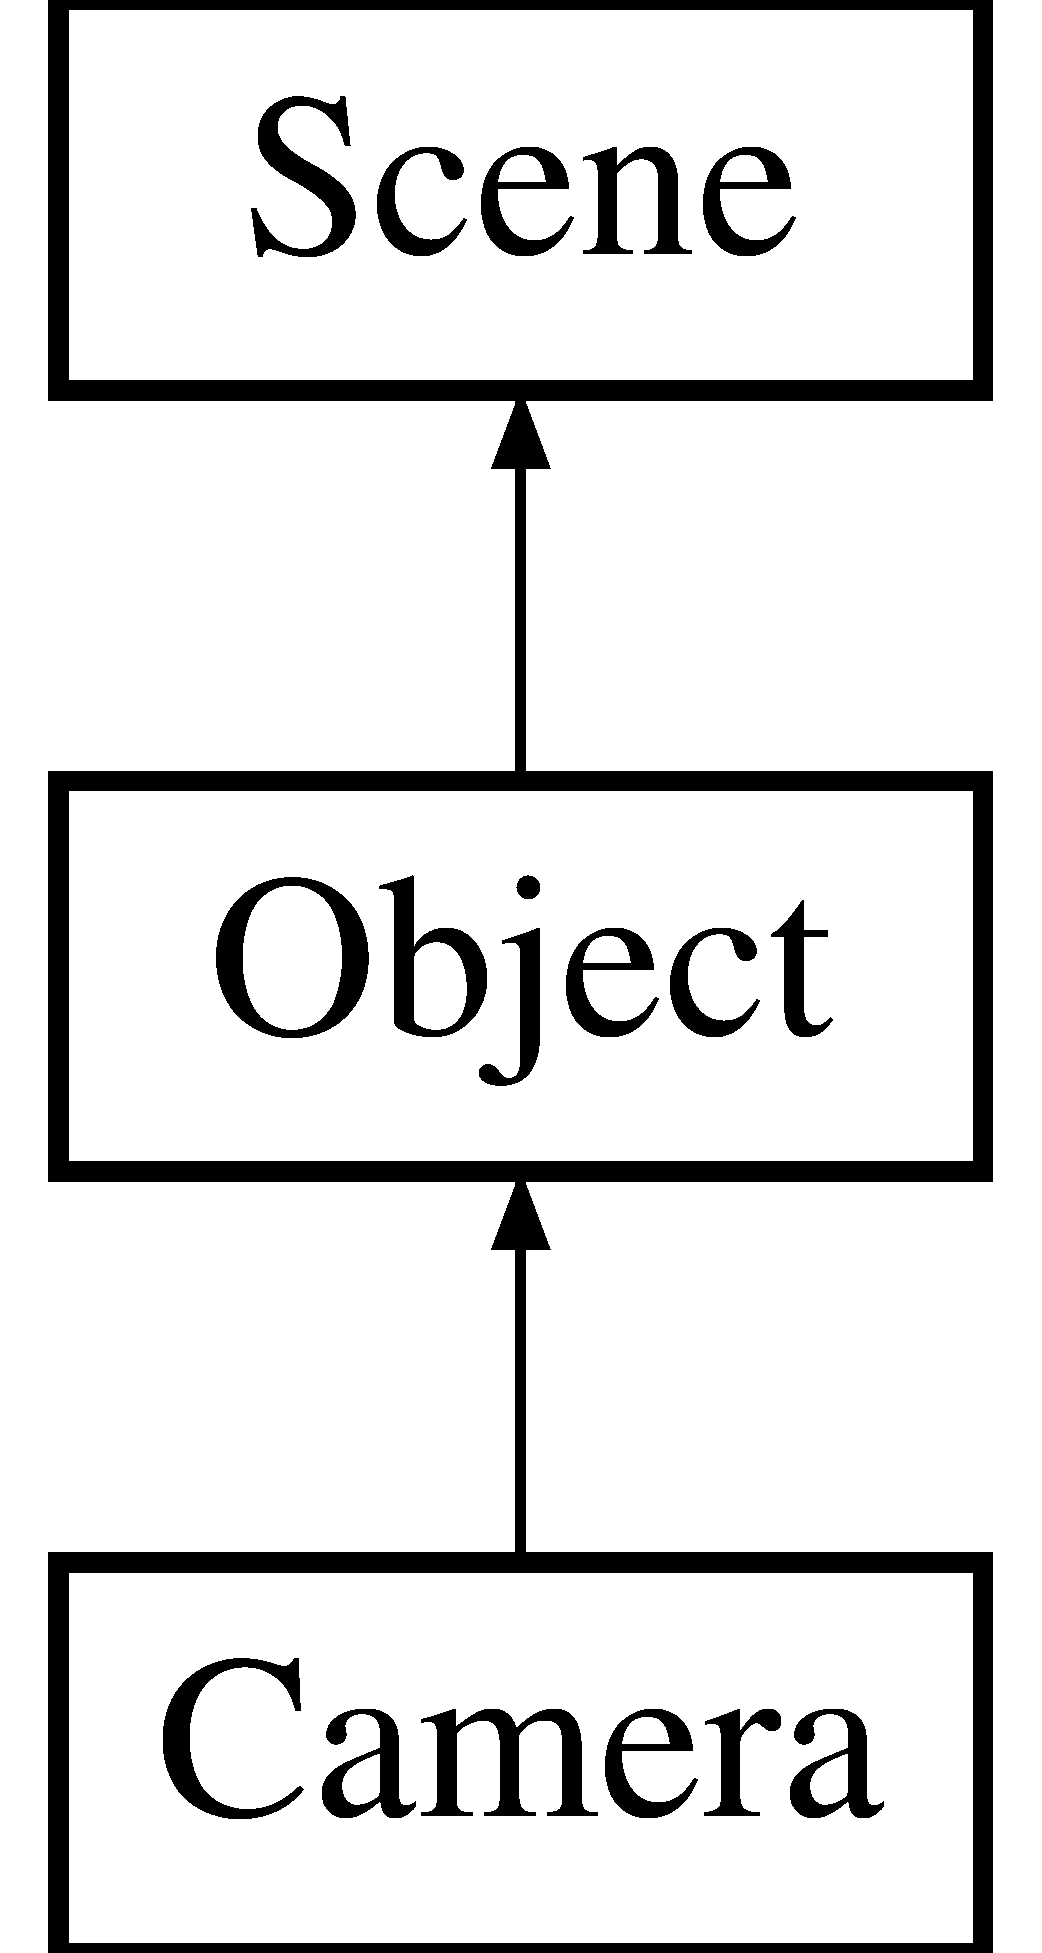
\includegraphics[height=3.000000cm]{class_camera}
\end{center}
\end{figure}
\subsection*{Public Types}
\begin{DoxyCompactItemize}
\item 
enum \hyperlink{class_camera_a80cb65605322d27ad3b6d973484509ec}{Direction} \{ \\*
{\bfseries D\-I\-R\-\_\-\-F\-O\-R\-W\-A\-R\-D}, 
{\bfseries D\-I\-R\-\_\-\-B\-A\-C\-K\-W\-A\-R\-D}, 
{\bfseries D\-I\-R\-\_\-\-L\-E\-F\-T}, 
{\bfseries D\-I\-R\-\_\-\-R\-I\-G\-H\-T}, 
\\*
{\bfseries D\-I\-R\-\_\-\-U\-P}, 
{\bfseries D\-I\-R\-\_\-\-D\-O\-W\-N}, 
{\bfseries D\-I\-R\-\_\-\-E\-N\-D}, 
{\bfseries D\-I\-R\-\_\-\-B\-E\-G\-I\-N} = D\-I\-R\-\_\-\-F\-O\-R\-W\-A\-R\-D
 \}
\begin{DoxyCompactList}\small\item\em The Direction enumeration lists all of the possible directions the camera may travel in. \end{DoxyCompactList}\item 
enum \hyperlink{class_camera_aaa256acd50a2fa143d9f8d9456e2802f}{View\-Type} \{ \\*
{\bfseries P\-E\-R\-S\-P\-E\-C\-T\-I\-V\-E}, 
{\bfseries O\-R\-T\-H\-O}, 
{\bfseries O\-R\-T\-H\-O2\-D}, 
{\bfseries I\-D\-E\-N\-T\-I\-T\-Y}, 
\\*
{\bfseries F\-R\-U\-S\-T\-U\-M}
 \}
\begin{DoxyCompactList}\small\item\em The View\-Type enumeration lists the various possibilities for the current viewing mode that can be switched between. \end{DoxyCompactList}\item 
enum \hyperlink{class_camera_a630738fd23098d44c0d15ee28d5649dd}{Uniforms} \{ \\*
{\bfseries B\-E\-G\-I\-N} = Object\-:\-:E\-N\-D, 
{\bfseries T\-R\-A\-N\-S\-L\-A\-T\-I\-O\-N} = B\-E\-G\-I\-N, 
{\bfseries R\-O\-T\-A\-T\-I\-O\-N}, 
{\bfseries V\-I\-E\-W}, 
\\*
{\bfseries C\-T\-M}, 
{\bfseries E\-N\-D}
 \}
\begin{DoxyCompactList}\small\item\em The glsl\-\_\-var enumeration lists the various variables the \hyperlink{class_camera}{Camera} class is capable of sending to the shader. \end{DoxyCompactList}\item 
typedef enum \hyperlink{class_camera_a80cb65605322d27ad3b6d973484509ec}{Camera\-::\-Direction} \hyperlink{class_camera_a94bb7ceb1c7a05e54cf638924f228baf}{Direction}
\begin{DoxyCompactList}\small\item\em The Direction enumeration lists all of the possible directions the camera may travel in. \end{DoxyCompactList}\item 
typedef enum \hyperlink{class_camera_aaa256acd50a2fa143d9f8d9456e2802f}{Camera\-::\-View\-Type} \hyperlink{class_camera_a5b2dc5eaed6cbaabee0eea3f2714acd7}{View\-Type}
\begin{DoxyCompactList}\small\item\em The View\-Type enumeration lists the various possibilities for the current viewing mode that can be switched between. \end{DoxyCompactList}\item 
typedef enum \hyperlink{class_camera_a630738fd23098d44c0d15ee28d5649dd}{Camera\-::\-Uniforms} \hyperlink{class_camera_a0ed19c96505cbb70625938d1e883af24}{Uniform}
\begin{DoxyCompactList}\small\item\em The glsl\-\_\-var enumeration lists the various variables the \hyperlink{class_camera}{Camera} class is capable of sending to the shader. \end{DoxyCompactList}\item 
typedef const unsigned int \hyperlink{class_object_a79b74057dbc5182b85c9c3ba8480fcf2}{Uniform\-Enum}
\begin{DoxyCompactList}\small\item\em The \hyperlink{class_object}{Object} class takes advantage of child-\/extendible enumerations. \end{DoxyCompactList}\item 
typedef std\-::map\\*
$<$ \hyperlink{class_object_a79b74057dbc5182b85c9c3ba8480fcf2}{Object\-::\-Uniform\-Enum}, \\*
std\-::string $>$ \hyperlink{class_object_a6e19bd8516360bff956408cbae33b878}{Uniform\-Map}
\begin{DoxyCompactList}\small\item\em We store mappings of Uniform Enumerations, The desired function of the var, to strings, the names of the variables. \end{DoxyCompactList}\end{DoxyCompactItemize}
\subsection*{Public Member Functions}
\begin{DoxyCompactItemize}
\item 
\hyperlink{class_camera_a16516fa8c830cecef5c8eb43eff12783}{Camera} (const std\-::string \&\hyperlink{class_object_aafd766fce2598f718cac97a3ac731706}{name}, G\-Luint g\-Shader, float \hyperlink{class_camera_a14d59ca64bf258adacbed4e0e70ba701}{x}=0.\-0, float \hyperlink{class_camera_a5021b8379a853f306851837178856db0}{y}=0.\-0, float \hyperlink{class_camera_a4acfa20291c83f13c98781c0d53cdbd8}{z}=0.\-0)
\begin{DoxyCompactList}\small\item\em Initialization Constructor; sets the x,y,z coordinates explicitly. \end{DoxyCompactList}\item 
\hyperlink{class_camera_a24329612384948d2b64f78094fe84e75}{Camera} (const std\-::string \&\hyperlink{class_object_aafd766fce2598f718cac97a3ac731706}{name}, G\-Luint g\-Shader, \hyperlink{struct_angel_1_1vec3}{vec3} \&in)
\begin{DoxyCompactList}\small\item\em Initialization Constructor, uses a vec3 as its initial coordinates. \end{DoxyCompactList}\item 
\hyperlink{class_camera_aa131bc7f1bad2cc8baea463714c4485d}{Camera} (const std\-::string \&\hyperlink{class_object_aafd766fce2598f718cac97a3ac731706}{name}, G\-Luint g\-Shader, \hyperlink{struct_angel_1_1vec4}{vec4} \&in)
\begin{DoxyCompactList}\small\item\em Initialization Constructor, uses a vec4 as its initial coordinates. \end{DoxyCompactList}\item 
virtual \hyperlink{class_camera_a06211f202c145b3ec8253f96e1e654a6}{$\sim$\-Camera} (void)
\begin{DoxyCompactList}\small\item\em Default destructor. \end{DoxyCompactList}\item 
void \hyperlink{class_camera_a14d59ca64bf258adacbed4e0e70ba701}{x} (const float \&in, const bool \&update=true)
\begin{DoxyCompactList}\small\item\em Sets the x coordinate of the camera. \end{DoxyCompactList}\item 
void \hyperlink{class_camera_a5021b8379a853f306851837178856db0}{y} (const float \&in, const bool \&update=true)
\begin{DoxyCompactList}\small\item\em Sets the y coordinate of the camera. \end{DoxyCompactList}\item 
void \hyperlink{class_camera_a4acfa20291c83f13c98781c0d53cdbd8}{z} (const float \&in, const bool \&update=true)
\begin{DoxyCompactList}\small\item\em Sets the z coordinate of the camera. \end{DoxyCompactList}\item 
void \hyperlink{class_camera_a432e03c15d63f8839fe4731016d907a4}{pos} (const float \&\hyperlink{class_camera_a14d59ca64bf258adacbed4e0e70ba701}{x}, const float \&\hyperlink{class_camera_a5021b8379a853f306851837178856db0}{y}, const float \&\hyperlink{class_camera_a4acfa20291c83f13c98781c0d53cdbd8}{z}, const bool \&update=true)
\begin{DoxyCompactList}\small\item\em Sets the absolute position of the camera. \end{DoxyCompactList}\item 
void \hyperlink{class_camera_ae9dc2206b71b25cf320a05d148cb8b56}{pos} (const \hyperlink{struct_angel_1_1vec3}{vec3} \&in, const bool \&update=true)
\begin{DoxyCompactList}\small\item\em Sets the absolute position of the camera. \end{DoxyCompactList}\item 
void \hyperlink{class_camera_aec2115038562e514193bb2b67f5da153}{pos} (const \hyperlink{struct_angel_1_1vec4}{vec4} \&in, const bool \&update=true)
\begin{DoxyCompactList}\small\item\em Sets the absolute position of the camera. \end{DoxyCompactList}\item 
void \hyperlink{class_camera_ac7985a6cb48f4e1e74fda17e5213dd74}{d\-X} (const float \&by, const bool \&update=true)
\begin{DoxyCompactList}\small\item\em Moves the camera along the x axis. \end{DoxyCompactList}\item 
void \hyperlink{class_camera_a59570a88e3ff2d277c9e995372fcadfe}{d\-Y} (const float \&by, const bool \&update=true)
\begin{DoxyCompactList}\small\item\em Moves the camera along the y axis. \end{DoxyCompactList}\item 
void \hyperlink{class_camera_ab94ed9b3c7e12f484d6bfa5f827b59ff}{d\-Z} (const float \&by, const bool \&update=true)
\begin{DoxyCompactList}\small\item\em Moves the camera along the z axis. \end{DoxyCompactList}\item 
void \hyperlink{class_camera_a2ac5f89b4f9f012dead66980925143c0}{d\-Pos} (const float \&\hyperlink{class_camera_a14d59ca64bf258adacbed4e0e70ba701}{x}, const float \&\hyperlink{class_camera_a5021b8379a853f306851837178856db0}{y}, const float \&\hyperlink{class_camera_a4acfa20291c83f13c98781c0d53cdbd8}{z})
\begin{DoxyCompactList}\small\item\em Moves the camera along the x, y, and z axes. \end{DoxyCompactList}\item 
void \hyperlink{class_camera_a928de59670f0b31264307a8a0888b99d}{d\-Pos} (const \hyperlink{struct_angel_1_1vec3}{vec3} \&by)
\begin{DoxyCompactList}\small\item\em Moves the camera along the x, y, and z axes. \end{DoxyCompactList}\item 
void \hyperlink{class_camera_a4ec2e3d2a66826aedb1ac1eee7da0b96}{d\-Pos} (const \hyperlink{struct_angel_1_1vec4}{vec4} \&by)
\begin{DoxyCompactList}\small\item\em Moves the camera along the x, y, and z axes. \end{DoxyCompactList}\item 
void \hyperlink{class_camera_a36ec0e0e832f789e27d42e7bd4f6d174}{field\-Of\-View} (const float \&fovy)
\begin{DoxyCompactList}\small\item\em field\-Of\-View sets the current camera Field-\/of-\/view angle. \end{DoxyCompactList}\item 
float \hyperlink{class_camera_a9b3675bf6866a67f8fa802bb4aecba89}{field\-Of\-View} (void) const 
\begin{DoxyCompactList}\small\item\em \hyperlink{class_camera_a9b3675bf6866a67f8fa802bb4aecba89}{field\-Of\-View()} gets the current camera Field-\/of-\/view angle. \end{DoxyCompactList}\item 
void \hyperlink{class_camera_a717f5d58bb0a73f8c5513a3520d98203}{adjust\-Field\-Of\-View} (const float \&by)
\begin{DoxyCompactList}\small\item\em adjust\-Field\-Of\-View adjusts the field of view angle up or down by an amount. \end{DoxyCompactList}\item 
void \hyperlink{class_camera_a8463a19c9e1e7a1c51cd97051e937230}{change\-Perspective} (const \hyperlink{class_camera_aaa256acd50a2fa143d9f8d9456e2802f}{View\-Type} \&v\-Type)
\begin{DoxyCompactList}\small\item\em change\-Perspective changes the current perspective of the camera. \end{DoxyCompactList}\item 
void \hyperlink{class_camera_a24c5346fc0dfaa93257b6716fe0f2421}{refresh\-Perspective} (void)
\begin{DoxyCompactList}\small\item\em refresh\-Perspective re-\/generates the current view/perspective matrix of the camera. \end{DoxyCompactList}\item 
void \hyperlink{class_camera_adda458a9212825164b52019597f2e9c8}{viewport} (size\-\_\-t \-\_\-\-X, size\-\_\-t \-\_\-\-Y, size\-\_\-t \-\_\-width, size\-\_\-t \-\_\-height)
\begin{DoxyCompactList}\small\item\em viewport instructs this camera what his expected drawing window will be. \end{DoxyCompactList}\item 
void \hyperlink{class_camera_abbe6fe82ed05e64e35b0c4ed2001b34e}{sway} (const float \&by)
\begin{DoxyCompactList}\small\item\em Adjusts the camera's x coordinate relative to its current position. \end{DoxyCompactList}\item 
void \hyperlink{class_camera_abb2251df65445bf8efd3fe0074fb5033}{surge} (const float \&by)
\begin{DoxyCompactList}\small\item\em Adjusts the camera's z coordinate relative to its current position. \end{DoxyCompactList}\item 
void \hyperlink{class_camera_a2148d751f104d8e39c9832e2372df2d9}{heave} (const float \&by)
\begin{DoxyCompactList}\small\item\em Adjusts the camera's y coordinate relative to its current position. \end{DoxyCompactList}\item 
void \hyperlink{class_camera_aac7dbb6201be7f17e014fc6fdf915560}{pitch} (const float \&by, const bool \&fixed=false)
\begin{DoxyCompactList}\small\item\em pitch adjusts the x axis rotation; up/down look. \end{DoxyCompactList}\item 
void \hyperlink{class_camera_a0ce7d12edbe47d9a8915d8af98d8f524}{yaw} (const float \&by, const bool \&fixed=false)
\begin{DoxyCompactList}\small\item\em yaw adjusts the y axis rotation; left/right look. \end{DoxyCompactList}\item 
void \hyperlink{class_camera_a1ba0979fe0b2ec58085d5f9721858e5e}{roll} (const float \&by, const bool \&fixed=false)
\begin{DoxyCompactList}\small\item\em roll adjusts the z axis rotation; tilt or lean left/right. \end{DoxyCompactList}\item 
void \hyperlink{class_camera_aaa9706527438bd5bd323dd018bb34fcf}{move} (const \hyperlink{class_camera_a80cb65605322d27ad3b6d973484509ec}{Camera\-::\-Direction} \&Dir)
\begin{DoxyCompactList}\small\item\em move instructs the camera to begin moving in the specified direction. \end{DoxyCompactList}\item 
void \hyperlink{class_camera_ae7414c6ae83c3c9392ab90e957daf2b9}{stop} (const \hyperlink{class_camera_a80cb65605322d27ad3b6d973484509ec}{Camera\-::\-Direction} \&Dir)
\begin{DoxyCompactList}\small\item\em stop instructs the camera to stop moving in the specified direction. \end{DoxyCompactList}\item 
void \hyperlink{class_camera_a9c620bd05c119791c080e479ee71abc2}{idle} (void)
\begin{DoxyCompactList}\small\item\em idle moves the camera forward in whichever directions it is configured to move in. \end{DoxyCompactList}\item 
void \hyperlink{class_camera_abee6a36602b8044478739cea9221ed41}{accel} (const \hyperlink{struct_angel_1_1vec3}{vec3} \&accel)
\begin{DoxyCompactList}\small\item\em accel takes an input vec2 which represents an acceleration, and applies it to the motion vectors with regards to the maximum acceleration and the maximum speed of the camera. \end{DoxyCompactList}\item 
float \hyperlink{class_camera_ab84abdd525581fbaf0462595d0a087d6}{x} (void) const 
\begin{DoxyCompactList}\small\item\em \hyperlink{class_camera_ab84abdd525581fbaf0462595d0a087d6}{x()} returns the current position of the camera in model coordinates. \end{DoxyCompactList}\item 
float \hyperlink{class_camera_a68d0865ed19510ee41c6477511d70185}{y} (void) const 
\begin{DoxyCompactList}\small\item\em \hyperlink{class_camera_a68d0865ed19510ee41c6477511d70185}{y()} returns the current position of the camera in model coordinates. \end{DoxyCompactList}\item 
float \hyperlink{class_camera_ab1167495c547046c57b1c417e53c39f6}{z} (void) const 
\begin{DoxyCompactList}\small\item\em \hyperlink{class_camera_ab1167495c547046c57b1c417e53c39f6}{z()} returns the current position of the camera in model coordinates. \end{DoxyCompactList}\item 
\hyperlink{struct_angel_1_1vec4}{vec4} \hyperlink{class_camera_a9982ac5f48fe0af97fefa725080d6da6}{pos} (void) const 
\begin{DoxyCompactList}\small\item\em \hyperlink{class_camera_a9982ac5f48fe0af97fefa725080d6da6}{pos()} gets the current camera position in model coordinates. \end{DoxyCompactList}\item 
virtual void \hyperlink{class_camera_a401decef27b59d6485b4ab9762f5b9e6}{send} (\hyperlink{class_object_a79b74057dbc5182b85c9c3ba8480fcf2}{Object\-::\-Uniform\-Enum} which)
\begin{DoxyCompactList}\small\item\em send will send a glsl variable to the shader. \end{DoxyCompactList}\item 
void \hyperlink{class_camera_ae845a36306bba6b6e359cbdddce65f7f}{view} (void)
\begin{DoxyCompactList}\small\item\em view will instruct Open\-G\-L of the viewport we want, and then send all of our current matrices to the shader for rendering. \end{DoxyCompactList}\item 
void \hyperlink{class_camera_a8ec7938c5e25068e5bff25aeb7038af4}{reset\-Rotation} (void)
\begin{DoxyCompactList}\small\item\em reset\-Rotation adjusts the camera's rotational state back to its default state (The Identity Matrix.) \end{DoxyCompactList}\item 
\hypertarget{class_object_a53e2ee7f548550be014126bed139fe69}{void \hyperlink{class_object_a53e2ee7f548550be014126bed139fe69}{draw} (void)}\label{class_object_a53e2ee7f548550be014126bed139fe69}

\begin{DoxyCompactList}\small\item\em draw method\-: Render this object to the screen \-\_\-buffer. \end{DoxyCompactList}\item 
\hypertarget{class_object_a7edb92c30d86b6479b0ff2a5e9f06e13}{void \hyperlink{class_object_a7edb92c30d86b6479b0ff2a5e9f06e13}{buffer} (void)}\label{class_object_a7edb92c30d86b6479b0ff2a5e9f06e13}

\begin{DoxyCompactList}\small\item\em buffer all of our data\-: Vertices, Tex\-U\-Vs, Normals, Indices, Colors and Morph Buffers. \end{DoxyCompactList}\item 
\hypertarget{class_object_a293792abfe0671e00a0ec10e85ea9d9e}{void \hyperlink{class_object_a293792abfe0671e00a0ec10e85ea9d9e}{buffer\-Morph\-Only} (void)}\label{class_object_a293792abfe0671e00a0ec10e85ea9d9e}

\begin{DoxyCompactList}\small\item\em buffer only the Morph-\/related buffers. \end{DoxyCompactList}\item 
void \hyperlink{class_object_adafdf22583b051b4c61c8eb725fb07d5}{draw\-Mode} (G\-Lenum new\-\_\-mode)
\begin{DoxyCompactList}\small\item\em Select a new Open\-G\-L draw mode for this \hyperlink{class_object}{Object}. \end{DoxyCompactList}\item 
void \hyperlink{class_object_afebb27ddb10daed8e2c5085b76cbc500}{texture} (const char $\ast$$\ast$filename)
\begin{DoxyCompactList}\small\item\em F\-I\-X\-M\-E\-: This is a junk, nonflexible method. \end{DoxyCompactList}\item 
const std\-::string \& \hyperlink{class_object_aafd766fce2598f718cac97a3ac731706}{name} (void) const 
\begin{DoxyCompactList}\small\item\em Retrieve the \-\_\-name of this \hyperlink{class_object}{Object}. \end{DoxyCompactList}\item 
virtual void \hyperlink{class_object_a11d6063c580331d6af59c8d71b7f3e9f}{link} (\hyperlink{class_object_a79b74057dbc5182b85c9c3ba8480fcf2}{Uniform\-Enum} which, const std\-::string \&\hyperlink{class_object_aafd766fce2598f718cac97a3ac731706}{name})
\begin{DoxyCompactList}\small\item\em link a specified Uniform against the shader's variable \-\_\-name. \end{DoxyCompactList}\item 
virtual G\-Luint \hyperlink{class_object_a459489106838a1e3a8dbbd13045cd523}{shader} (void)
\begin{DoxyCompactList}\small\item\em Returns the \hyperlink{class_object}{Object}'s current shader. \end{DoxyCompactList}\item 
virtual void \hyperlink{class_object_aeaf11bb87bd59381c9e066f0b4f40d8e}{shader} (G\-Luint new\-Shader)
\begin{DoxyCompactList}\small\item\em Sets the shader to be used by this object. \end{DoxyCompactList}\item 
void \hyperlink{class_object_a0d604a816115c474b9593aeaebda9f8b}{animation} (void($\ast$anim\-\_\-func)(\hyperlink{class_trans_cache}{Trans\-Cache} \&arg))
\begin{DoxyCompactList}\small\item\em Apply an animation callback function to this \hyperlink{class_object}{Object}. \end{DoxyCompactList}\item 
void \hyperlink{class_object_a70a0f93ad9805057c5cc39853ce049c7}{propegate} (void)
\begin{DoxyCompactList}\small\item\em Scene-\/graph changes are not automatically applied to children. \end{DoxyCompactList}\item 
\hyperlink{struct_angel_1_1vec4}{vec4} \hyperlink{class_object_ac64609eb614aa5974b74000cec6fc95c}{position} () const 
\begin{DoxyCompactList}\small\item\em Obtain the vec4 representative of the \hyperlink{class_object}{Object}'s current position in space. \end{DoxyCompactList}\item 
\hyperlink{class_object}{Object} $\ast$ \hyperlink{class_object_a7694c9cfe445c3d5b993a38e3f8badd9}{morph\-Target} () const 
\begin{DoxyCompactList}\small\item\em Retrieve a pointer to this object's morph target. \end{DoxyCompactList}\item 
\hyperlink{class_object}{Object} $\ast$ \hyperlink{class_object_ab0ba603904f8f7de15dc0450e2d9b30e}{gen\-Morph\-Target} (G\-Luint \hyperlink{class_object_a459489106838a1e3a8dbbd13045cd523}{shader})
\begin{DoxyCompactList}\small\item\em Instantiate a new morphing target. \end{DoxyCompactList}\item 
float \hyperlink{class_object_accb051cdc79bc93e8c9c0edb79dd6b30}{morph\-Percentage} () const 
\begin{DoxyCompactList}\small\item\em Retrieve the morph Percentage of this object. \end{DoxyCompactList}\item 
void \hyperlink{class_object_a543d2329b25df9fb0a782f09d03e5cb1}{morph\-Percentage} (const float new\-Percentage)
\begin{DoxyCompactList}\small\item\em Set the morph percentage of this \hyperlink{class_object}{Object}. \end{DoxyCompactList}\item 
\hypertarget{class_object_a98d3f1b9ebb61c3b21e2a59ed267480a}{void \hyperlink{class_object_a98d3f1b9ebb61c3b21e2a59ed267480a}{destroy\-Morph\-Target} ()}\label{class_object_a98d3f1b9ebb61c3b21e2a59ed267480a}

\begin{DoxyCompactList}\small\item\em Obliterate the morph target for this object. \end{DoxyCompactList}\item 
int \hyperlink{class_object_a73f1a6210bacf504de9a808009479b81}{number\-Of\-Points} ()
\begin{DoxyCompactList}\small\item\em Retrieve the number of \-\_\-vertices this object has. \end{DoxyCompactList}\item 
\hypertarget{class_scene_aa5a48614e959c38c35d824fa9d6a4b8b}{\hyperlink{class_object}{Object} $\ast$ {\bfseries add\-Object} (const std\-::string \&obj\-Name, G\-Luint Object\-\_\-\-Shader=0)}\label{class_scene_aa5a48614e959c38c35d824fa9d6a4b8b}

\item 
\hypertarget{class_scene_a2a6845dacbb468c5c097c7a6ab5a0fe0}{void {\bfseries del\-Object} (const std\-::string \&obj\-Name)}\label{class_scene_a2a6845dacbb468c5c097c7a6ab5a0fe0}

\item 
\hypertarget{class_scene_a2e6b319b60e27e66ad43bb942a6c4424}{void {\bfseries del\-Object} (void)}\label{class_scene_a2e6b319b60e27e66ad43bb942a6c4424}

\item 
\hypertarget{class_scene_ad6c9d1d1d0c786d39bf97dc60410e28b}{void {\bfseries pop\-Object} (void)}\label{class_scene_ad6c9d1d1d0c786d39bf97dc60410e28b}

\item 
\hypertarget{class_scene_a8c57e1cebc39586c7928225d1e25de39}{void \hyperlink{class_scene_a8c57e1cebc39586c7928225d1e25de39}{destroy\-Object} (void)}\label{class_scene_a8c57e1cebc39586c7928225d1e25de39}

\begin{DoxyCompactList}\small\item\em Completely remove this object and all his children. \end{DoxyCompactList}\item 
\hypertarget{class_scene_a70fcdad192a4c6ff508125de8af6cf4d}{\hyperlink{class_object}{Object} $\ast$ {\bfseries next} (void)}\label{class_scene_a70fcdad192a4c6ff508125de8af6cf4d}

\item 
\hypertarget{class_scene_ac852d5d763eb35b4908c9aa7ea54d1ae}{\hyperlink{class_object}{Object} $\ast$ {\bfseries prev} (void)}\label{class_scene_ac852d5d763eb35b4908c9aa7ea54d1ae}

\item 
\hypertarget{class_scene_ad0ea1a6bcf7815c63988bd937f06eb23}{\hyperlink{class_object}{Object} $\ast$ {\bfseries active} (void) const }\label{class_scene_ad0ea1a6bcf7815c63988bd937f06eb23}

\item 
\hypertarget{class_scene_ae9b69d8db8a46991017635f22e45baad}{\hyperlink{class_object}{Object} $\ast$ {\bfseries operator\mbox{[}$\,$\mbox{]}} (const std\-::string \&objname)}\label{class_scene_ae9b69d8db8a46991017635f22e45baad}

\end{DoxyCompactItemize}
\subsection*{Public Attributes}
\begin{DoxyCompactItemize}
\item 
std\-::vector$<$ \hyperlink{struct_angel_1_1vec4}{Angel\-::vec4} $>$ \hyperlink{class_object_a4ac354b3ec284f27358b1d4b8d95b9a9}{\-\_\-vertices}
\begin{DoxyCompactList}\small\item\em vertex buffer. \end{DoxyCompactList}\item 
std\-::vector$<$ \hyperlink{struct_angel_1_1vec3}{Angel\-::vec3} $>$ \hyperlink{class_object_a20bb786cb5915934853855aab9d1a1b3}{\-\_\-normals}
\begin{DoxyCompactList}\small\item\em Normals buffer. \end{DoxyCompactList}\item 
std\-::vector$<$ unsigned int $>$ \hyperlink{class_object_ab85adc7a2d3b891051c096593982653d}{\-\_\-indices}
\begin{DoxyCompactList}\small\item\em Draw Order Index buffer. \end{DoxyCompactList}\item 
std\-::vector$<$ \hyperlink{struct_angel_1_1vec4}{Angel\-::vec4} $>$ \hyperlink{class_object_a29a0e9959c490067db69378bf57a17ba}{\-\_\-colors}
\begin{DoxyCompactList}\small\item\em Colors buffer. \end{DoxyCompactList}\item 
std\-::vector$<$ \hyperlink{struct_angel_1_1vec2}{Angel\-::vec2} $>$ \hyperlink{class_object_aa9ddc3b95d74b76ab8a251fb376dfafb}{\-\_\-tex\-U\-Vs}
\begin{DoxyCompactList}\small\item\em Texture Coordinates buffer. \end{DoxyCompactList}\item 
\hypertarget{class_object_af17d57ea2dab64e21112e8949d50d85f}{\hyperlink{class_trans_cache}{Trans\-Cache} \hyperlink{class_object_af17d57ea2dab64e21112e8949d50d85f}{\-\_\-trans}}\label{class_object_af17d57ea2dab64e21112e8949d50d85f}

\begin{DoxyCompactList}\small\item\em The \-\_\-trans cache encompasses the current transformational state of this object. \end{DoxyCompactList}\end{DoxyCompactItemize}
\subsection*{Protected Member Functions}
\begin{DoxyCompactItemize}
\item 
void \hyperlink{class_scene_ad3897f8ac658af62c133783b2c4eaee4}{delete\-Object} (\hyperlink{class_object}{Object} $\ast$obj)
\begin{DoxyCompactList}\small\item\em delete\-Object is the actual implementation function that will remove an \hyperlink{class_object}{Object} from the \hyperlink{class_scene}{Scene} list and \hyperlink{class_scene}{Scene} map, then free the object. \end{DoxyCompactList}\item 
\hypertarget{class_scene_ab64354bd8059bab589ca2dbf9de9e66c}{void {\bfseries insert\-Object} (const std\-::string \hyperlink{class_object_aafd766fce2598f718cac97a3ac731706}{name}, \hyperlink{class_object}{Object} $\ast$obj)}\label{class_scene_ab64354bd8059bab589ca2dbf9de9e66c}

\end{DoxyCompactItemize}
\subsection*{Protected Attributes}
\begin{DoxyCompactItemize}
\item 
std\-::string \hyperlink{class_object_a3f617214b260ebbe394e7c7b08ab5e43}{\-\_\-name}
\begin{DoxyCompactList}\small\item\em \-\_\-name is used as an identifying handle for the object. \end{DoxyCompactList}\item 
G\-Luint \hyperlink{class_object_a564aa6b1df66a05ab6b6c2f071851c4e}{\-\_\-vao}
\begin{DoxyCompactList}\small\item\em Vertex Array \hyperlink{class_object}{Object} handle identifying our buffers/object. \end{DoxyCompactList}\item 
\hypertarget{class_object_adf8365e2c661ab4014c3dbf60e48572b}{G\-Luint \hyperlink{class_object_adf8365e2c661ab4014c3dbf60e48572b}{\-\_\-buffer} \mbox{[}\hyperlink{class_object_a74a39247838865244defd0ae9712df9ba1999a38dc687c7ae05c884078de39b51}{N\-U\-M\-\_\-\-B\-U\-F\-F\-E\-R\-S}\mbox{]}}\label{class_object_adf8365e2c661ab4014c3dbf60e48572b}

\begin{DoxyCompactList}\small\item\em Handles to our buffers (Vertices, Tex\-U\-Vs, etc.) \end{DoxyCompactList}\item 
G\-Lenum \hyperlink{class_object_ae8457eabfb89d55826142508013b56c0}{\-\_\-draw\-Mode}
\begin{DoxyCompactList}\small\item\em Drawing mode for this object. \end{DoxyCompactList}\item 
\hypertarget{class_object_abcb877094b696561a49bc931c5a12d9f}{bool \hyperlink{class_object_abcb877094b696561a49bc931c5a12d9f}{\-\_\-is\-Textured}}\label{class_object_abcb877094b696561a49bc931c5a12d9f}

\begin{DoxyCompactList}\small\item\em Is this object textured? \end{DoxyCompactList}\item 
float \hyperlink{class_object_a7fbbac9027e1a8266342bd5ce064120d}{\-\_\-morph\-Percentage}
\begin{DoxyCompactList}\small\item\em The percentage of the morph. \end{DoxyCompactList}\item 
\hypertarget{class_object_a5baa9891bd4981d62b4e86a1c2a8eea7}{\hyperlink{class_object}{Object} $\ast$ \hyperlink{class_object_a5baa9891bd4981d62b4e86a1c2a8eea7}{\-\_\-morph\-Target}}\label{class_object_a5baa9891bd4981d62b4e86a1c2a8eea7}

\begin{DoxyCompactList}\small\item\em A pointer to the object we wish to morph into. \end{DoxyCompactList}\item 
std\-::map$<$ \hyperlink{class_object_a79b74057dbc5182b85c9c3ba8480fcf2}{Object\-::\-Uniform\-Enum}, \\*
std\-::string $>$ \hyperlink{class_object_a6378d0b0eeec23045ae2a5245e42bf13}{\-\_\-uniform\-Map}
\begin{DoxyCompactList}\small\item\em A map between Uniform variable functions and the actual uniform variable names. \end{DoxyCompactList}\item 
std\-::vector$<$ G\-Lint $>$ \hyperlink{class_object_a983963f564898beca4bda99676245663}{\-\_\-handles}
\begin{DoxyCompactList}\small\item\em Handles to Uniforms on the shader. \end{DoxyCompactList}\item 
\hypertarget{class_scene_acdd0123ca6b2d64d8d447bb485b235fc}{std\-::list$<$ \hyperlink{class_object}{Object} $\ast$ $>$ {\bfseries \-\_\-list}}\label{class_scene_acdd0123ca6b2d64d8d447bb485b235fc}

\item 
\hypertarget{class_scene_a8bd5d86484a12255b26b92b6cbf8d29a}{std\-::map$<$ std\-::string, \hyperlink{class_object}{Object} $\ast$ $>$ {\bfseries \-\_\-map}}\label{class_scene_a8bd5d86484a12255b26b92b6cbf8d29a}

\item 
\hypertarget{class_scene_ae87ca5350fcc595f3f15a4fd3c39f3d9}{std\-::list$<$ \hyperlink{class_object}{Object} $\ast$ $>$\-::iterator {\bfseries \-\_\-current\-Obj}}\label{class_scene_ae87ca5350fcc595f3f15a4fd3c39f3d9}

\item 
\hypertarget{class_scene_a8f9bdd8ec5edb1f414fbd314a36e2724}{G\-Luint {\bfseries \-\_\-g\-Shader}}\label{class_scene_a8f9bdd8ec5edb1f414fbd314a36e2724}

\end{DoxyCompactItemize}
\subsection*{Private Member Functions}
\begin{DoxyCompactItemize}
\item 
void \hyperlink{class_camera_aba32f195cdb5bfcfd05c2ce74315b6c3}{adjust\-Rotation} (const \hyperlink{class_angel_1_1mat4}{mat4} \&adjustment, const bool \&fixed=false)
\begin{DoxyCompactList}\small\item\em adjust\-Rotation is an internal function that rotates the camera. \end{DoxyCompactList}\item 
void \hyperlink{class_camera_a20243a7e3eb06ab1265118c5fb9cce9b}{common\-Init} (void)
\begin{DoxyCompactList}\small\item\em common\-Init is a private function that initializes local object attributes. \end{DoxyCompactList}\end{DoxyCompactItemize}
\subsection*{Private Attributes}
\begin{DoxyCompactItemize}
\item 
\hyperlink{class_angel_1_1mat4}{mat4} \hyperlink{class_camera_a28f6e710df6db726568cd0f2bbd3643a}{\-\_\-view}
\begin{DoxyCompactList}\small\item\em The current view matrix (defaultly perspective) for this camera. \end{DoxyCompactList}\item 
\hyperlink{class_trans_cache}{Trans\-Cache} \hyperlink{class_camera_a6c1e31c8470b923f9f872f73597cb95b}{\-\_\-ctm}
\begin{DoxyCompactList}\small\item\em The Current \hyperlink{class_transformation}{Transformation} state for this \hyperlink{class_camera}{Camera}. \end{DoxyCompactList}\item 
\hyperlink{class_camera_aaa256acd50a2fa143d9f8d9456e2802f}{View\-Type} \hyperlink{class_camera_ac9062d9bb891aa81d163076738451081}{\-\_\-current\-View}
\begin{DoxyCompactList}\small\item\em The current viewing mode type. \end{DoxyCompactList}\item 
G\-Lfloat \hyperlink{class_camera_a21f8eb53e5369018e39add0453ae626d}{\-\_\-speed}
\begin{DoxyCompactList}\small\item\em Current Speed of camera motion. \end{DoxyCompactList}\item 
\hyperlink{struct_angel_1_1vec3}{vec3} \hyperlink{class_camera_aa15577ff9e67c81699ee86d4d20a7ee7}{\-\_\-velocity}
\begin{DoxyCompactList}\small\item\em Current Velocity of camera motion. \end{DoxyCompactList}\item 
\hypertarget{class_camera_a4d875d29a43bdfed4eac4c76747939d3}{G\-Lfloat \hyperlink{class_camera_a4d875d29a43bdfed4eac4c76747939d3}{\-\_\-speed\-\_\-cap}}\label{class_camera_a4d875d29a43bdfed4eac4c76747939d3}

\begin{DoxyCompactList}\small\item\em Current Speed Capacity\-: (speed/\-Max\-Speed) \end{DoxyCompactList}\item 
\hypertarget{class_camera_acbfae99c73c118ca92be9a6ba664b303}{G\-Lfloat \hyperlink{class_camera_acbfae99c73c118ca92be9a6ba664b303}{\-\_\-max\-Accel}}\label{class_camera_acbfae99c73c118ca92be9a6ba664b303}

\begin{DoxyCompactList}\small\item\em Maximum Acceleration Magnitude. \end{DoxyCompactList}\item 
\hypertarget{class_camera_a83cab43f9ccc3d5f4c7db8543a806745}{G\-Lfloat \hyperlink{class_camera_a83cab43f9ccc3d5f4c7db8543a806745}{\-\_\-max\-Speed}}\label{class_camera_a83cab43f9ccc3d5f4c7db8543a806745}

\begin{DoxyCompactList}\small\item\em Maximum Speed. \end{DoxyCompactList}\item 
G\-Lfloat \hyperlink{class_camera_a66fb66da0ccd400c4986dc19276b6716}{\-\_\-friction\-Magnitude}
\begin{DoxyCompactList}\small\item\em Friction. \end{DoxyCompactList}\item 
G\-Lfloat \hyperlink{class_camera_a42082e8f2d80a13674ce163d8e720bfb}{\-\_\-aspect\-Ratio}
\begin{DoxyCompactList}\small\item\em Current aspect ratio for certain perspectives. \end{DoxyCompactList}\item 
G\-Lfloat \hyperlink{class_camera_a82542bb76347e2a2bb66b3bb7842945b}{\-\_\-fovy}
\begin{DoxyCompactList}\small\item\em Current field-\/of-\/view angle for perspective view. \end{DoxyCompactList}\item 
\hypertarget{class_camera_a67c7600162abef1d2cddfce8cc75c33b}{\hyperlink{struct_angel_1_1vec2}{Angel\-::vec2} \hyperlink{class_camera_a67c7600162abef1d2cddfce8cc75c33b}{\-\_\-viewport\-Size}}\label{class_camera_a67c7600162abef1d2cddfce8cc75c33b}

\begin{DoxyCompactList}\small\item\em \hyperlink{class_camera}{Camera}'s Drawbox Width and Height. \end{DoxyCompactList}\item 
\hypertarget{class_camera_adb7506be3632abc2d33e77a5783f5be8}{\hyperlink{struct_angel_1_1vec2}{Angel\-::vec2} \hyperlink{class_camera_adb7506be3632abc2d33e77a5783f5be8}{\-\_\-viewport\-Position}}\label{class_camera_adb7506be3632abc2d33e77a5783f5be8}

\begin{DoxyCompactList}\small\item\em \hyperlink{class_camera}{Camera}'s Drawbox x,y Coordinate (Upper-\/\-Left Pixel) \end{DoxyCompactList}\item 
bool \hyperlink{class_camera_abec7e2becbad5a692a54a69b6a5f6d75}{\-\_\-motion} \mbox{[}Camera\-::\-D\-I\-R\-\_\-\-E\-N\-D\mbox{]}
\begin{DoxyCompactList}\small\item\em Booleans correlating to the different motion directions. \end{DoxyCompactList}\end{DoxyCompactItemize}


\subsection{Detailed Description}
The \hyperlink{class_camera}{Camera} class represents a logical camera in a model view, which posesses a current viewing angle and an absolute position in space as its state. 

\begin{DoxyAuthor}{Author}
John Huston, \href{mailto:jhuston@cs.uml.edu}{\tt jhuston@cs.\-uml.\-edu} 
\end{DoxyAuthor}
\begin{DoxySince}{Since}
16 Nov 2012
\end{DoxySince}
Functions are provided to adjust the rotation according to \hyperlink{class_camera_aac7dbb6201be7f17e014fc6fdf915560}{pitch()}, \hyperlink{class_camera_a0ce7d12edbe47d9a8915d8af98d8f524}{yaw()} and \hyperlink{class_camera_a1ba0979fe0b2ec58085d5f9721858e5e}{roll()} motions; \hyperlink{class_camera_abb2251df65445bf8efd3fe0074fb5033}{surge()}, \hyperlink{class_camera_abbe6fe82ed05e64e35b0c4ed2001b34e}{sway()}, and \hyperlink{class_camera_a2148d751f104d8e39c9832e2372df2d9}{heave()} are provided to adjust position in space.

\hyperlink{class_camera_aaa9706527438bd5bd323dd018bb34fcf}{move()}, \hyperlink{class_camera_ae7414c6ae83c3c9392ab90e957daf2b9}{stop()}, and \hyperlink{class_camera_a9c620bd05c119791c080e479ee71abc2}{idle()} are provided to help the camera automatically move along the x, y, or z axes. 

Definition at line 37 of file Camera.\-hpp.



\subsection{Member Typedef Documentation}
\hypertarget{class_camera_a94bb7ceb1c7a05e54cf638924f228baf}{\index{Camera@{Camera}!Direction@{Direction}}
\index{Direction@{Direction}!Camera@{Camera}}
\subsubsection[{Direction}]{\setlength{\rightskip}{0pt plus 5cm}typedef enum {\bf Camera\-::\-Direction}  {\bf Camera\-::\-Direction}}}\label{class_camera_a94bb7ceb1c7a05e54cf638924f228baf}


The Direction enumeration lists all of the possible directions the camera may travel in. 

'B\-E\-G\-I\-N' and 'E\-N\-D' are special sentinel directions for the purposes of iteration, and are ignored by any functions that accept a Direction. \hypertarget{class_camera_a0ed19c96505cbb70625938d1e883af24}{\index{Camera@{Camera}!Uniform@{Uniform}}
\index{Uniform@{Uniform}!Camera@{Camera}}
\subsubsection[{Uniform}]{\setlength{\rightskip}{0pt plus 5cm}typedef enum {\bf Camera\-::\-Uniforms}  {\bf Camera\-::\-Uniform}}}\label{class_camera_a0ed19c96505cbb70625938d1e883af24}


The glsl\-\_\-var enumeration lists the various variables the \hyperlink{class_camera}{Camera} class is capable of sending to the shader. 

The Num\-Glsl\-Vars variable is a sentinel value that is ignored by any functions that accept a glsl\-\_\-var. \hypertarget{class_object_a79b74057dbc5182b85c9c3ba8480fcf2}{\index{Camera@{Camera}!Uniform\-Enum@{Uniform\-Enum}}
\index{Uniform\-Enum@{Uniform\-Enum}!Camera@{Camera}}
\subsubsection[{Uniform\-Enum}]{\setlength{\rightskip}{0pt plus 5cm}typedef const unsigned int {\bf Object\-::\-Uniform\-Enum}\hspace{0.3cm}{\ttfamily [inherited]}}}\label{class_object_a79b74057dbc5182b85c9c3ba8480fcf2}


The \hyperlink{class_object}{Object} class takes advantage of child-\/extendible enumerations. 

We create an alias here for sake of ease. 

Definition at line 62 of file Object.\-hpp.

\hypertarget{class_object_a6e19bd8516360bff956408cbae33b878}{\index{Camera@{Camera}!Uniform\-Map@{Uniform\-Map}}
\index{Uniform\-Map@{Uniform\-Map}!Camera@{Camera}}
\subsubsection[{Uniform\-Map}]{\setlength{\rightskip}{0pt plus 5cm}typedef std\-::map$<$ {\bf Object\-::\-Uniform\-Enum}, std\-::string $>$ {\bf Object\-::\-Uniform\-Map}\hspace{0.3cm}{\ttfamily [inherited]}}}\label{class_object_a6e19bd8516360bff956408cbae33b878}


We store mappings of Uniform Enumerations, The desired function of the var, to strings, the names of the variables. 

This is utilized if we ever switch this object's shader, so we can re-\/associate with the correct uniform locations. 

Definition at line 70 of file Object.\-hpp.

\hypertarget{class_camera_a5b2dc5eaed6cbaabee0eea3f2714acd7}{\index{Camera@{Camera}!View\-Type@{View\-Type}}
\index{View\-Type@{View\-Type}!Camera@{Camera}}
\subsubsection[{View\-Type}]{\setlength{\rightskip}{0pt plus 5cm}typedef enum {\bf Camera\-::\-View\-Type}  {\bf Camera\-::\-View\-Type}}}\label{class_camera_a5b2dc5eaed6cbaabee0eea3f2714acd7}


The View\-Type enumeration lists the various possibilities for the current viewing mode that can be switched between. 

The default is P\-E\-R\-S\-P\-E\-C\-T\-I\-V\-E. 

\subsection{Member Enumeration Documentation}
\hypertarget{class_camera_a80cb65605322d27ad3b6d973484509ec}{\index{Camera@{Camera}!Direction@{Direction}}
\index{Direction@{Direction}!Camera@{Camera}}
\subsubsection[{Direction}]{\setlength{\rightskip}{0pt plus 5cm}enum {\bf Camera\-::\-Direction}}}\label{class_camera_a80cb65605322d27ad3b6d973484509ec}


The Direction enumeration lists all of the possible directions the camera may travel in. 

'B\-E\-G\-I\-N' and 'E\-N\-D' are special sentinel directions for the purposes of iteration, and are ignored by any functions that accept a Direction. 

Definition at line 47 of file Camera.\-hpp.

\hypertarget{class_camera_a630738fd23098d44c0d15ee28d5649dd}{\index{Camera@{Camera}!Uniforms@{Uniforms}}
\index{Uniforms@{Uniforms}!Camera@{Camera}}
\subsubsection[{Uniforms}]{\setlength{\rightskip}{0pt plus 5cm}enum {\bf Camera\-::\-Uniforms}}}\label{class_camera_a630738fd23098d44c0d15ee28d5649dd}


The glsl\-\_\-var enumeration lists the various variables the \hyperlink{class_camera}{Camera} class is capable of sending to the shader. 

The Num\-Glsl\-Vars variable is a sentinel value that is ignored by any functions that accept a glsl\-\_\-var. 

Definition at line 73 of file Camera.\-hpp.

\hypertarget{class_camera_aaa256acd50a2fa143d9f8d9456e2802f}{\index{Camera@{Camera}!View\-Type@{View\-Type}}
\index{View\-Type@{View\-Type}!Camera@{Camera}}
\subsubsection[{View\-Type}]{\setlength{\rightskip}{0pt plus 5cm}enum {\bf Camera\-::\-View\-Type}}}\label{class_camera_aaa256acd50a2fa143d9f8d9456e2802f}


The View\-Type enumeration lists the various possibilities for the current viewing mode that can be switched between. 

The default is P\-E\-R\-S\-P\-E\-C\-T\-I\-V\-E. 

Definition at line 63 of file Camera.\-hpp.



\subsection{Constructor \& Destructor Documentation}
\hypertarget{class_camera_a16516fa8c830cecef5c8eb43eff12783}{\index{Camera@{Camera}!Camera@{Camera}}
\index{Camera@{Camera}!Camera@{Camera}}
\subsubsection[{Camera}]{\setlength{\rightskip}{0pt plus 5cm}Camera\-::\-Camera (
\begin{DoxyParamCaption}
\item[{const std\-::string \&}]{name, }
\item[{G\-Luint}]{g\-Shader, }
\item[{float}]{x = {\ttfamily 0.0}, }
\item[{float}]{y = {\ttfamily 0.0}, }
\item[{float}]{z = {\ttfamily 0.0}}
\end{DoxyParamCaption}
)}}\label{class_camera_a16516fa8c830cecef5c8eb43eff12783}


Initialization Constructor; sets the x,y,z coordinates explicitly. 


\begin{DoxyParams}{Parameters}
{\em name} & The name of this Camera/\-Object. \\
\hline
{\em g\-Shader} & A handle to this camera's associated shader object. \\
\hline
{\em x} & The initial x coordinate. \\
\hline
{\em y} & The initial y coordinate. \\
\hline
{\em z} & The initial z coordinate. \\
\hline
\end{DoxyParams}


Definition at line 45 of file Camera.\-cpp.

\hypertarget{class_camera_a24329612384948d2b64f78094fe84e75}{\index{Camera@{Camera}!Camera@{Camera}}
\index{Camera@{Camera}!Camera@{Camera}}
\subsubsection[{Camera}]{\setlength{\rightskip}{0pt plus 5cm}Camera\-::\-Camera (
\begin{DoxyParamCaption}
\item[{const std\-::string \&}]{name, }
\item[{G\-Luint}]{g\-Shader, }
\item[{{\bf vec3} \&}]{in}
\end{DoxyParamCaption}
)}}\label{class_camera_a24329612384948d2b64f78094fe84e75}


Initialization Constructor, uses a vec3 as its initial coordinates. 


\begin{DoxyParams}{Parameters}
{\em name} & The name of this Camera/\-Object. \\
\hline
{\em g\-Shader} & A handle to this camera's associated shader object. \\
\hline
{\em in} & A vec3 representing the initial coordinates. \\
\hline
\end{DoxyParams}


Definition at line 52 of file Camera.\-cpp.

\hypertarget{class_camera_aa131bc7f1bad2cc8baea463714c4485d}{\index{Camera@{Camera}!Camera@{Camera}}
\index{Camera@{Camera}!Camera@{Camera}}
\subsubsection[{Camera}]{\setlength{\rightskip}{0pt plus 5cm}Camera\-::\-Camera (
\begin{DoxyParamCaption}
\item[{const std\-::string \&}]{name, }
\item[{G\-Luint}]{g\-Shader, }
\item[{{\bf vec4} \&}]{in}
\end{DoxyParamCaption}
)}}\label{class_camera_aa131bc7f1bad2cc8baea463714c4485d}


Initialization Constructor, uses a vec4 as its initial coordinates. 


\begin{DoxyParams}{Parameters}
{\em name} & The name of this Camera/\-Object. \\
\hline
{\em g\-Shader} & A handle to this camera's associated shader object. \\
\hline
{\em in} & A vec4 representing the initial coordinates. The w component is ignored. \\
\hline
\end{DoxyParams}


Definition at line 58 of file Camera.\-cpp.

\hypertarget{class_camera_a06211f202c145b3ec8253f96e1e654a6}{\index{Camera@{Camera}!$\sim$\-Camera@{$\sim$\-Camera}}
\index{$\sim$\-Camera@{$\sim$\-Camera}!Camera@{Camera}}
\subsubsection[{$\sim$\-Camera}]{\setlength{\rightskip}{0pt plus 5cm}Camera\-::$\sim$\-Camera (
\begin{DoxyParamCaption}
\item[{void}]{}
\end{DoxyParamCaption}
)\hspace{0.3cm}{\ttfamily [virtual]}}}\label{class_camera_a06211f202c145b3ec8253f96e1e654a6}


Default destructor. 

Defined only to allow inheritance. 

Definition at line 64 of file Camera.\-cpp.



\subsection{Member Function Documentation}
\hypertarget{class_camera_abee6a36602b8044478739cea9221ed41}{\index{Camera@{Camera}!accel@{accel}}
\index{accel@{accel}!Camera@{Camera}}
\subsubsection[{accel}]{\setlength{\rightskip}{0pt plus 5cm}void Camera\-::accel (
\begin{DoxyParamCaption}
\item[{const {\bf vec3} \&}]{accel}
\end{DoxyParamCaption}
)}}\label{class_camera_abee6a36602b8044478739cea9221ed41}


accel takes an input vec2 which represents an acceleration, and applies it to the motion vectors with regards to the maximum acceleration and the maximum speed of the camera. 


\begin{DoxyParams}{Parameters}
{\em accel} & The vec3 which represents the (x,y,z) acceleration, where x,y,z are \mbox{[}-\/1,1\mbox{]}. \\
\hline
\end{DoxyParams}
\begin{DoxyReturn}{Returns}
Void. 
\end{DoxyReturn}


Definition at line 223 of file Camera.\-cpp.

\hypertarget{class_camera_a717f5d58bb0a73f8c5513a3520d98203}{\index{Camera@{Camera}!adjust\-Field\-Of\-View@{adjust\-Field\-Of\-View}}
\index{adjust\-Field\-Of\-View@{adjust\-Field\-Of\-View}!Camera@{Camera}}
\subsubsection[{adjust\-Field\-Of\-View}]{\setlength{\rightskip}{0pt plus 5cm}void Camera\-::adjust\-Field\-Of\-View (
\begin{DoxyParamCaption}
\item[{const float \&}]{by}
\end{DoxyParamCaption}
)}}\label{class_camera_a717f5d58bb0a73f8c5513a3520d98203}


adjust\-Field\-Of\-View adjusts the field of view angle up or down by an amount. 


\begin{DoxyParams}{Parameters}
{\em by} & The float to adjust the field\-Of\-View angle by. \\
\hline
\end{DoxyParams}
\begin{DoxyReturn}{Returns}
Void. 
\end{DoxyReturn}


Definition at line 392 of file Camera.\-cpp.

\hypertarget{class_camera_aba32f195cdb5bfcfd05c2ce74315b6c3}{\index{Camera@{Camera}!adjust\-Rotation@{adjust\-Rotation}}
\index{adjust\-Rotation@{adjust\-Rotation}!Camera@{Camera}}
\subsubsection[{adjust\-Rotation}]{\setlength{\rightskip}{0pt plus 5cm}void Camera\-::adjust\-Rotation (
\begin{DoxyParamCaption}
\item[{const {\bf mat4} \&}]{adjustment, }
\item[{const bool \&}]{fixed = {\ttfamily false}}
\end{DoxyParamCaption}
)\hspace{0.3cm}{\ttfamily [private]}}}\label{class_camera_aba32f195cdb5bfcfd05c2ce74315b6c3}


adjust\-Rotation is an internal function that rotates the camera. 

Technically, any transformation, not just a rotation, is possible. 
\begin{DoxyParams}{Parameters}
{\em adjustment} & The 4x4 matrix to transform the C\-T\-M by. \\
\hline
{\em fixed} & Should this rotation be fixed about the origin? \\
\hline
\end{DoxyParams}
\begin{DoxyReturn}{Returns}
Void. 
\end{DoxyReturn}


Definition at line 148 of file Camera.\-cpp.

\hypertarget{class_object_a0d604a816115c474b9593aeaebda9f8b}{\index{Camera@{Camera}!animation@{animation}}
\index{animation@{animation}!Camera@{Camera}}
\subsubsection[{animation}]{\setlength{\rightskip}{0pt plus 5cm}void Object\-::animation (
\begin{DoxyParamCaption}
\item[{void($\ast$)({\bf Trans\-Cache} \&arg)}]{anim\-\_\-func}
\end{DoxyParamCaption}
)\hspace{0.3cm}{\ttfamily [inherited]}}}\label{class_object_a0d604a816115c474b9593aeaebda9f8b}


Apply an animation callback function to this \hyperlink{class_object}{Object}. 

Works once only\-: Does not save the function or automatically run on idle. 
\begin{DoxyParams}{Parameters}
{\em anim\-\_\-func} & The transformation/animation function to apply. \\
\hline
\end{DoxyParams}


Definition at line 485 of file Object.\-cpp.

\hypertarget{class_camera_a8463a19c9e1e7a1c51cd97051e937230}{\index{Camera@{Camera}!change\-Perspective@{change\-Perspective}}
\index{change\-Perspective@{change\-Perspective}!Camera@{Camera}}
\subsubsection[{change\-Perspective}]{\setlength{\rightskip}{0pt plus 5cm}void Camera\-::change\-Perspective (
\begin{DoxyParamCaption}
\item[{const {\bf View\-Type} \&}]{v\-Type}
\end{DoxyParamCaption}
)}}\label{class_camera_a8463a19c9e1e7a1c51cd97051e937230}


change\-Perspective changes the current perspective of the camera. 


\begin{DoxyParams}{Parameters}
{\em v\-Type} & Which perspective to use. see enum View\-Type for possibilities. \\
\hline
\end{DoxyParams}
\begin{DoxyReturn}{Returns}
Void. 
\end{DoxyReturn}


Definition at line 359 of file Camera.\-cpp.

\hypertarget{class_camera_a20243a7e3eb06ab1265118c5fb9cce9b}{\index{Camera@{Camera}!common\-Init@{common\-Init}}
\index{common\-Init@{common\-Init}!Camera@{Camera}}
\subsubsection[{common\-Init}]{\setlength{\rightskip}{0pt plus 5cm}void Camera\-::common\-Init (
\begin{DoxyParamCaption}
\item[{void}]{}
\end{DoxyParamCaption}
)\hspace{0.3cm}{\ttfamily [private]}}}\label{class_camera_a20243a7e3eb06ab1265118c5fb9cce9b}


common\-Init is a private function that initializes local object attributes. 

It should be called by all available constructors. \begin{DoxyReturn}{Returns}
Void. 
\end{DoxyReturn}


Definition at line 19 of file Camera.\-cpp.

\hypertarget{class_scene_ad3897f8ac658af62c133783b2c4eaee4}{\index{Camera@{Camera}!delete\-Object@{delete\-Object}}
\index{delete\-Object@{delete\-Object}!Camera@{Camera}}
\subsubsection[{delete\-Object}]{\setlength{\rightskip}{0pt plus 5cm}void Scene\-::delete\-Object (
\begin{DoxyParamCaption}
\item[{{\bf Object} $\ast$}]{obj}
\end{DoxyParamCaption}
)\hspace{0.3cm}{\ttfamily [protected]}, {\ttfamily [inherited]}}}\label{class_scene_ad3897f8ac658af62c133783b2c4eaee4}


delete\-Object is the actual implementation function that will remove an \hyperlink{class_object}{Object} from the \hyperlink{class_scene}{Scene} list and \hyperlink{class_scene}{Scene} map, then free the object. 


\begin{DoxyParams}{Parameters}
{\em obj} & The pointer to the object to free. \\
\hline
\end{DoxyParams}


Definition at line 76 of file Scene.\-cpp.

\hypertarget{class_camera_a2ac5f89b4f9f012dead66980925143c0}{\index{Camera@{Camera}!d\-Pos@{d\-Pos}}
\index{d\-Pos@{d\-Pos}!Camera@{Camera}}
\subsubsection[{d\-Pos}]{\setlength{\rightskip}{0pt plus 5cm}void Camera\-::d\-Pos (
\begin{DoxyParamCaption}
\item[{const float \&}]{x, }
\item[{const float \&}]{y, }
\item[{const float \&}]{z}
\end{DoxyParamCaption}
)}}\label{class_camera_a2ac5f89b4f9f012dead66980925143c0}


Moves the camera along the x, y, and z axes. 


\begin{DoxyParams}{Parameters}
{\em x} & the x-\/axis displacement. \\
\hline
{\em y} & the y-\/axis displacement. \\
\hline
{\em z} & the z-\/axis displacement. \\
\hline
\end{DoxyParams}
\begin{DoxyReturn}{Returns}
Void. 
\end{DoxyReturn}


Definition at line 131 of file Camera.\-cpp.

\hypertarget{class_camera_a928de59670f0b31264307a8a0888b99d}{\index{Camera@{Camera}!d\-Pos@{d\-Pos}}
\index{d\-Pos@{d\-Pos}!Camera@{Camera}}
\subsubsection[{d\-Pos}]{\setlength{\rightskip}{0pt plus 5cm}void Camera\-::d\-Pos (
\begin{DoxyParamCaption}
\item[{const {\bf vec3} \&}]{by}
\end{DoxyParamCaption}
)}}\label{class_camera_a928de59670f0b31264307a8a0888b99d}


Moves the camera along the x, y, and z axes. 


\begin{DoxyParams}{Parameters}
{\em by} & A vec3 containing the x, y, and z axis displacements. \\
\hline
\end{DoxyParams}
\begin{DoxyReturn}{Returns}
Void. 
\end{DoxyReturn}


Definition at line 140 of file Camera.\-cpp.

\hypertarget{class_camera_a4ec2e3d2a66826aedb1ac1eee7da0b96}{\index{Camera@{Camera}!d\-Pos@{d\-Pos}}
\index{d\-Pos@{d\-Pos}!Camera@{Camera}}
\subsubsection[{d\-Pos}]{\setlength{\rightskip}{0pt plus 5cm}void Camera\-::d\-Pos (
\begin{DoxyParamCaption}
\item[{const {\bf vec4} \&}]{by}
\end{DoxyParamCaption}
)}}\label{class_camera_a4ec2e3d2a66826aedb1ac1eee7da0b96}


Moves the camera along the x, y, and z axes. 


\begin{DoxyParams}{Parameters}
{\em by} & A vec4 containing the x, y, and z axis displacements. The w component is ignored. \\
\hline
\end{DoxyParams}
\begin{DoxyReturn}{Returns}
Void. 
\end{DoxyReturn}


Definition at line 144 of file Camera.\-cpp.

\hypertarget{class_object_adafdf22583b051b4c61c8eb725fb07d5}{\index{Camera@{Camera}!draw\-Mode@{draw\-Mode}}
\index{draw\-Mode@{draw\-Mode}!Camera@{Camera}}
\subsubsection[{draw\-Mode}]{\setlength{\rightskip}{0pt plus 5cm}void Object\-::draw\-Mode (
\begin{DoxyParamCaption}
\item[{G\-Lenum}]{new\-\_\-mode}
\end{DoxyParamCaption}
)\hspace{0.3cm}{\ttfamily [inherited]}}}\label{class_object_adafdf22583b051b4c61c8eb725fb07d5}


Select a new Open\-G\-L draw mode for this \hyperlink{class_object}{Object}. 

Can be G\-L\-\_\-\-L\-I\-N\-E\-S, G\-L\-\_\-\-L\-I\-N\-E\-\_\-\-L\-O\-O\-P, G\-L\-\_\-\-T\-R\-I\-A\-N\-G\-L\-E\-S, etc. \begin{DoxySeeAlso}{See Also}
\href{http://www.opengl.org/wiki/Primitive}{\tt http\-://www.\-opengl.\-org/wiki/\-Primitive} 
\end{DoxySeeAlso}

\begin{DoxyParams}{Parameters}
{\em new\-\_\-mode} & The primitive rendering mode to use. \\
\hline
\end{DoxyParams}


Definition at line 267 of file Object.\-cpp.

\hypertarget{class_camera_ac7985a6cb48f4e1e74fda17e5213dd74}{\index{Camera@{Camera}!d\-X@{d\-X}}
\index{d\-X@{d\-X}!Camera@{Camera}}
\subsubsection[{d\-X}]{\setlength{\rightskip}{0pt plus 5cm}void Camera\-::d\-X (
\begin{DoxyParamCaption}
\item[{const float \&}]{by, }
\item[{const bool \&}]{update = {\ttfamily true}}
\end{DoxyParamCaption}
)}}\label{class_camera_ac7985a6cb48f4e1e74fda17e5213dd74}


Moves the camera along the x axis. 


\begin{DoxyParams}{Parameters}
{\em by} & The float value of the x-\/axis displacement. \\
\hline
{\em update} & A boolean indicating whether or not to update the shader. update defaults to true. \\
\hline
\end{DoxyParams}
\begin{DoxyReturn}{Returns}
void. 
\end{DoxyReturn}


Definition at line 119 of file Camera.\-cpp.

\hypertarget{class_camera_a59570a88e3ff2d277c9e995372fcadfe}{\index{Camera@{Camera}!d\-Y@{d\-Y}}
\index{d\-Y@{d\-Y}!Camera@{Camera}}
\subsubsection[{d\-Y}]{\setlength{\rightskip}{0pt plus 5cm}void Camera\-::d\-Y (
\begin{DoxyParamCaption}
\item[{const float \&}]{by, }
\item[{const bool \&}]{update = {\ttfamily true}}
\end{DoxyParamCaption}
)}}\label{class_camera_a59570a88e3ff2d277c9e995372fcadfe}


Moves the camera along the y axis. 


\begin{DoxyParams}{Parameters}
{\em by} & The float value of the y-\/axis displacement. \\
\hline
{\em update} & A boolean indicating whether or not to update the shader. update defaults to true. \\
\hline
\end{DoxyParams}
\begin{DoxyReturn}{Returns}
Void. 
\end{DoxyReturn}


Definition at line 123 of file Camera.\-cpp.

\hypertarget{class_camera_ab94ed9b3c7e12f484d6bfa5f827b59ff}{\index{Camera@{Camera}!d\-Z@{d\-Z}}
\index{d\-Z@{d\-Z}!Camera@{Camera}}
\subsubsection[{d\-Z}]{\setlength{\rightskip}{0pt plus 5cm}void Camera\-::d\-Z (
\begin{DoxyParamCaption}
\item[{const float \&}]{by, }
\item[{const bool \&}]{update = {\ttfamily true}}
\end{DoxyParamCaption}
)}}\label{class_camera_ab94ed9b3c7e12f484d6bfa5f827b59ff}


Moves the camera along the z axis. 


\begin{DoxyParams}{Parameters}
{\em by} & The float value of the z-\/axis displacement. \\
\hline
{\em update} & A boolean indicating whether or not to update the shader. update defaults to true. \\
\hline
\end{DoxyParams}
\begin{DoxyReturn}{Returns}
Void. 
\end{DoxyReturn}


Definition at line 127 of file Camera.\-cpp.

\hypertarget{class_camera_a36ec0e0e832f789e27d42e7bd4f6d174}{\index{Camera@{Camera}!field\-Of\-View@{field\-Of\-View}}
\index{field\-Of\-View@{field\-Of\-View}!Camera@{Camera}}
\subsubsection[{field\-Of\-View}]{\setlength{\rightskip}{0pt plus 5cm}void Camera\-::field\-Of\-View (
\begin{DoxyParamCaption}
\item[{const float \&}]{fovy}
\end{DoxyParamCaption}
)}}\label{class_camera_a36ec0e0e832f789e27d42e7bd4f6d174}


field\-Of\-View sets the current camera Field-\/of-\/view angle. 

This function will send the new perspective matrix to the shader. 
\begin{DoxyParams}{Parameters}
{\em fovy} & The new field of view angle. \\
\hline
\end{DoxyParams}
\begin{DoxyReturn}{Returns}
Void. 
\end{DoxyReturn}


Definition at line 354 of file Camera.\-cpp.

\hypertarget{class_camera_a9b3675bf6866a67f8fa802bb4aecba89}{\index{Camera@{Camera}!field\-Of\-View@{field\-Of\-View}}
\index{field\-Of\-View@{field\-Of\-View}!Camera@{Camera}}
\subsubsection[{field\-Of\-View}]{\setlength{\rightskip}{0pt plus 5cm}float Camera\-::field\-Of\-View (
\begin{DoxyParamCaption}
\item[{void}]{}
\end{DoxyParamCaption}
) const}}\label{class_camera_a9b3675bf6866a67f8fa802bb4aecba89}


\hyperlink{class_camera_a9b3675bf6866a67f8fa802bb4aecba89}{field\-Of\-View()} gets the current camera Field-\/of-\/view angle. 

\begin{DoxyReturn}{Returns}
A float that is the y axis viewing angle. 
\end{DoxyReturn}


Definition at line 350 of file Camera.\-cpp.

\hypertarget{class_object_ab0ba603904f8f7de15dc0450e2d9b30e}{\index{Camera@{Camera}!gen\-Morph\-Target@{gen\-Morph\-Target}}
\index{gen\-Morph\-Target@{gen\-Morph\-Target}!Camera@{Camera}}
\subsubsection[{gen\-Morph\-Target}]{\setlength{\rightskip}{0pt plus 5cm}{\bf Object} $\ast$ Object\-::gen\-Morph\-Target (
\begin{DoxyParamCaption}
\item[{G\-Luint}]{shader}
\end{DoxyParamCaption}
)\hspace{0.3cm}{\ttfamily [inherited]}}}\label{class_object_ab0ba603904f8f7de15dc0450e2d9b30e}


Instantiate a new morphing target. 


\begin{DoxyParams}{Parameters}
{\em shader} & The shader to use for the new morphing target. N\-O\-T U\-S\-E\-D for rendering the object, but Objects cannot be instantiated without a shader, so here it is.\\
\hline
\end{DoxyParams}
\begin{DoxyReturn}{Returns}
A pointer to the newly created target. 
\end{DoxyReturn}


Definition at line 545 of file Object.\-cpp.

\hypertarget{class_camera_a2148d751f104d8e39c9832e2372df2d9}{\index{Camera@{Camera}!heave@{heave}}
\index{heave@{heave}!Camera@{Camera}}
\subsubsection[{heave}]{\setlength{\rightskip}{0pt plus 5cm}void Camera\-::heave (
\begin{DoxyParamCaption}
\item[{const float \&}]{by}
\end{DoxyParamCaption}
)}}\label{class_camera_a2148d751f104d8e39c9832e2372df2d9}


Adjusts the camera's y coordinate relative to its current position. 

Positive values move the camera up, and negative values move the camera down. 
\begin{DoxyParams}{Parameters}
{\em by} & The float to adjust the y coordinate by. \\
\hline
\end{DoxyParams}
\begin{DoxyReturn}{Returns}
Void. 
\end{DoxyReturn}


Definition at line 194 of file Camera.\-cpp.

\hypertarget{class_camera_a9c620bd05c119791c080e479ee71abc2}{\index{Camera@{Camera}!idle@{idle}}
\index{idle@{idle}!Camera@{Camera}}
\subsubsection[{idle}]{\setlength{\rightskip}{0pt plus 5cm}void Camera\-::idle (
\begin{DoxyParamCaption}
\item[{void}]{}
\end{DoxyParamCaption}
)}}\label{class_camera_a9c620bd05c119791c080e479ee71abc2}


idle moves the camera forward in whichever directions it is configured to move in. 

Call it in the glut idle function. \begin{DoxyReturn}{Returns}
Void. 
\end{DoxyReturn}


Definition at line 280 of file Camera.\-cpp.

\hypertarget{class_object_a11d6063c580331d6af59c8d71b7f3e9f}{\index{Camera@{Camera}!link@{link}}
\index{link@{link}!Camera@{Camera}}
\subsubsection[{link}]{\setlength{\rightskip}{0pt plus 5cm}void Object\-::link (
\begin{DoxyParamCaption}
\item[{{\bf Uniform\-Enum}}]{which, }
\item[{const std\-::string \&}]{name}
\end{DoxyParamCaption}
)\hspace{0.3cm}{\ttfamily [virtual]}, {\ttfamily [inherited]}}}\label{class_object_a11d6063c580331d6af59c8d71b7f3e9f}


link a specified Uniform against the shader's variable \-\_\-name. 


\begin{DoxyParams}{Parameters}
{\em which} & The Uniform to link. \\
\hline
{\em name} & The variable \-\_\-name on the shader. \\
\hline
\end{DoxyParams}


Definition at line 392 of file Object.\-cpp.

\hypertarget{class_object_accb051cdc79bc93e8c9c0edb79dd6b30}{\index{Camera@{Camera}!morph\-Percentage@{morph\-Percentage}}
\index{morph\-Percentage@{morph\-Percentage}!Camera@{Camera}}
\subsubsection[{morph\-Percentage}]{\setlength{\rightskip}{0pt plus 5cm}float Object\-::morph\-Percentage (
\begin{DoxyParamCaption}
\item[{void}]{}
\end{DoxyParamCaption}
) const\hspace{0.3cm}{\ttfamily [inherited]}}}\label{class_object_accb051cdc79bc93e8c9c0edb79dd6b30}


Retrieve the morph Percentage of this object. 

\begin{DoxyReturn}{Returns}
The morph percentage, as a float. 
\end{DoxyReturn}


Definition at line 557 of file Object.\-cpp.

\hypertarget{class_object_a543d2329b25df9fb0a782f09d03e5cb1}{\index{Camera@{Camera}!morph\-Percentage@{morph\-Percentage}}
\index{morph\-Percentage@{morph\-Percentage}!Camera@{Camera}}
\subsubsection[{morph\-Percentage}]{\setlength{\rightskip}{0pt plus 5cm}void Object\-::morph\-Percentage (
\begin{DoxyParamCaption}
\item[{const float}]{new\-Percentage}
\end{DoxyParamCaption}
)\hspace{0.3cm}{\ttfamily [inherited]}}}\label{class_object_a543d2329b25df9fb0a782f09d03e5cb1}


Set the morph percentage of this \hyperlink{class_object}{Object}. 


\begin{DoxyParams}{Parameters}
{\em new\-Percentage} & The new morphing percentage. \\
\hline
\end{DoxyParams}


Definition at line 566 of file Object.\-cpp.

\hypertarget{class_object_a7694c9cfe445c3d5b993a38e3f8badd9}{\index{Camera@{Camera}!morph\-Target@{morph\-Target}}
\index{morph\-Target@{morph\-Target}!Camera@{Camera}}
\subsubsection[{morph\-Target}]{\setlength{\rightskip}{0pt plus 5cm}{\bf Object} $\ast$ Object\-::morph\-Target (
\begin{DoxyParamCaption}
\item[{void}]{}
\end{DoxyParamCaption}
) const\hspace{0.3cm}{\ttfamily [inherited]}}}\label{class_object_a7694c9cfe445c3d5b993a38e3f8badd9}


Retrieve a pointer to this object's morph target. 

\begin{DoxyReturn}{Returns}
An \hyperlink{class_object}{Object} pointer to the morph target. 
\end{DoxyReturn}


Definition at line 531 of file Object.\-cpp.

\hypertarget{class_camera_aaa9706527438bd5bd323dd018bb34fcf}{\index{Camera@{Camera}!move@{move}}
\index{move@{move}!Camera@{Camera}}
\subsubsection[{move}]{\setlength{\rightskip}{0pt plus 5cm}void Camera\-::move (
\begin{DoxyParamCaption}
\item[{const {\bf Camera\-::\-Direction} \&}]{Dir}
\end{DoxyParamCaption}
)}}\label{class_camera_aaa9706527438bd5bd323dd018bb34fcf}


move instructs the camera to begin moving in the specified direction. 


\begin{DoxyParams}{Parameters}
{\em Dir} & The direction in which to move. Can be any direction in the enumerated type \hyperlink{class_camera_a80cb65605322d27ad3b6d973484509ec}{Camera\-::\-Direction}. \\
\hline
\end{DoxyParams}
\begin{DoxyReturn}{Returns}
Void. 
\end{DoxyReturn}


Definition at line 272 of file Camera.\-cpp.

\hypertarget{class_object_aafd766fce2598f718cac97a3ac731706}{\index{Camera@{Camera}!name@{name}}
\index{name@{name}!Camera@{Camera}}
\subsubsection[{name}]{\setlength{\rightskip}{0pt plus 5cm}const std\-::string \& Object\-::name (
\begin{DoxyParamCaption}
\item[{void}]{}
\end{DoxyParamCaption}
) const\hspace{0.3cm}{\ttfamily [inherited]}}}\label{class_object_aafd766fce2598f718cac97a3ac731706}


Retrieve the \-\_\-name of this \hyperlink{class_object}{Object}. 

\begin{DoxyReturn}{Returns}
The \-\_\-name of this \hyperlink{class_object}{Object}. 
\end{DoxyReturn}


Definition at line 380 of file Object.\-cpp.

\hypertarget{class_object_a73f1a6210bacf504de9a808009479b81}{\index{Camera@{Camera}!number\-Of\-Points@{number\-Of\-Points}}
\index{number\-Of\-Points@{number\-Of\-Points}!Camera@{Camera}}
\subsubsection[{number\-Of\-Points}]{\setlength{\rightskip}{0pt plus 5cm}int Object\-::number\-Of\-Points (
\begin{DoxyParamCaption}
\item[{void}]{}
\end{DoxyParamCaption}
)\hspace{0.3cm}{\ttfamily [inherited]}}}\label{class_object_a73f1a6210bacf504de9a808009479b81}


Retrieve the number of \-\_\-vertices this object has. 

\begin{DoxyReturn}{Returns}
An integer representing the number of vertices the object has. 
\end{DoxyReturn}


Definition at line 586 of file Object.\-cpp.

\hypertarget{class_camera_aac7dbb6201be7f17e014fc6fdf915560}{\index{Camera@{Camera}!pitch@{pitch}}
\index{pitch@{pitch}!Camera@{Camera}}
\subsubsection[{pitch}]{\setlength{\rightskip}{0pt plus 5cm}void Camera\-::pitch (
\begin{DoxyParamCaption}
\item[{const float \&}]{by, }
\item[{const bool \&}]{fixed = {\ttfamily false}}
\end{DoxyParamCaption}
)}}\label{class_camera_aac7dbb6201be7f17e014fc6fdf915560}


pitch adjusts the x axis rotation; up/down look. 

A positive value represents looking up, while a negative value represents looking down. 
\begin{DoxyParams}{Parameters}
{\em by} & A float, in degrees, to adjust the pitch by. \\
\hline
{\em fixed} & Should this rotation be fixed about the origin? \\
\hline
\end{DoxyParams}
\begin{DoxyReturn}{Returns}
Void. 
\end{DoxyReturn}


Definition at line 198 of file Camera.\-cpp.

\hypertarget{class_camera_a432e03c15d63f8839fe4731016d907a4}{\index{Camera@{Camera}!pos@{pos}}
\index{pos@{pos}!Camera@{Camera}}
\subsubsection[{pos}]{\setlength{\rightskip}{0pt plus 5cm}void Camera\-::pos (
\begin{DoxyParamCaption}
\item[{const float \&}]{x, }
\item[{const float \&}]{y, }
\item[{const float \&}]{z, }
\item[{const bool \&}]{update = {\ttfamily true}}
\end{DoxyParamCaption}
)}}\label{class_camera_a432e03c15d63f8839fe4731016d907a4}


Sets the absolute position of the camera. 


\begin{DoxyParams}{Parameters}
{\em x} & The new x coordinate of the camera. \\
\hline
{\em y} & The new y coordinate of the camera. \\
\hline
{\em z} & The new z coordinate of the camera. \\
\hline
{\em update} & Whether or not to update the shader with the new coordinates. \\
\hline
\end{DoxyParams}
\begin{DoxyReturn}{Returns}
Void. 
\end{DoxyReturn}


Definition at line 99 of file Camera.\-cpp.

\hypertarget{class_camera_ae9dc2206b71b25cf320a05d148cb8b56}{\index{Camera@{Camera}!pos@{pos}}
\index{pos@{pos}!Camera@{Camera}}
\subsubsection[{pos}]{\setlength{\rightskip}{0pt plus 5cm}void Camera\-::pos (
\begin{DoxyParamCaption}
\item[{const {\bf vec3} \&}]{in, }
\item[{const bool \&}]{update = {\ttfamily true}}
\end{DoxyParamCaption}
)}}\label{class_camera_ae9dc2206b71b25cf320a05d148cb8b56}


Sets the absolute position of the camera. 


\begin{DoxyParams}{Parameters}
{\em in} & A vec3 containing the x, y, and z coordinates to set the camera to. \\
\hline
{\em update} & Whether or not to update the shader with the new coordinates. \\
\hline
\end{DoxyParams}
\begin{DoxyReturn}{Returns}
Void. 
\end{DoxyReturn}


Definition at line 115 of file Camera.\-cpp.

\hypertarget{class_camera_aec2115038562e514193bb2b67f5da153}{\index{Camera@{Camera}!pos@{pos}}
\index{pos@{pos}!Camera@{Camera}}
\subsubsection[{pos}]{\setlength{\rightskip}{0pt plus 5cm}void Camera\-::pos (
\begin{DoxyParamCaption}
\item[{const {\bf vec4} \&}]{in, }
\item[{const bool \&}]{update = {\ttfamily true}}
\end{DoxyParamCaption}
)}}\label{class_camera_aec2115038562e514193bb2b67f5da153}


Sets the absolute position of the camera. 


\begin{DoxyParams}{Parameters}
{\em in} & A vec4 containing the x, y, and z coordinates to set the camera to. The w coordinate is ignored. \\
\hline
{\em update} & Whether or not to update the shader with the new coordinates. \\
\hline
\end{DoxyParams}
\begin{DoxyReturn}{Returns}
Void. 
\end{DoxyReturn}


Definition at line 111 of file Camera.\-cpp.

\hypertarget{class_camera_a9982ac5f48fe0af97fefa725080d6da6}{\index{Camera@{Camera}!pos@{pos}}
\index{pos@{pos}!Camera@{Camera}}
\subsubsection[{pos}]{\setlength{\rightskip}{0pt plus 5cm}{\bf vec4} Camera\-::pos (
\begin{DoxyParamCaption}
\item[{void}]{}
\end{DoxyParamCaption}
) const}}\label{class_camera_a9982ac5f48fe0af97fefa725080d6da6}


\hyperlink{class_camera_a9982ac5f48fe0af97fefa725080d6da6}{pos()} gets the current camera position in model coordinates. 

\begin{DoxyReturn}{Returns}
A vec4 that represents the current camera coordinates. 
\end{DoxyReturn}


Definition at line 346 of file Camera.\-cpp.

\hypertarget{class_object_ac64609eb614aa5974b74000cec6fc95c}{\index{Camera@{Camera}!position@{position}}
\index{position@{position}!Camera@{Camera}}
\subsubsection[{position}]{\setlength{\rightskip}{0pt plus 5cm}{\bf vec4} Object\-::position (
\begin{DoxyParamCaption}
\item[{void}]{}
\end{DoxyParamCaption}
) const\hspace{0.3cm}{\ttfamily [inherited]}}}\label{class_object_ac64609eb614aa5974b74000cec6fc95c}


Obtain the vec4 representative of the \hyperlink{class_object}{Object}'s current position in space. 

\begin{DoxyReturn}{Returns}
vec4 representing the \hyperlink{class_object}{Object}'s position in space. 
\end{DoxyReturn}


Definition at line 520 of file Object.\-cpp.

\hypertarget{class_object_a70a0f93ad9805057c5cc39853ce049c7}{\index{Camera@{Camera}!propegate@{propegate}}
\index{propegate@{propegate}!Camera@{Camera}}
\subsubsection[{propegate}]{\setlength{\rightskip}{0pt plus 5cm}void Object\-::propegate (
\begin{DoxyParamCaption}
\item[{void}]{}
\end{DoxyParamCaption}
)\hspace{0.3cm}{\ttfamily [inherited]}}}\label{class_object_a70a0f93ad9805057c5cc39853ce049c7}


Scene-\/graph changes are not automatically applied to children. 

For efficiency reasons, you need to call \hyperlink{class_object_a70a0f93ad9805057c5cc39853ce049c7}{propegate()} manually. 

Definition at line 494 of file Object.\-cpp.

\hypertarget{class_camera_a24c5346fc0dfaa93257b6716fe0f2421}{\index{Camera@{Camera}!refresh\-Perspective@{refresh\-Perspective}}
\index{refresh\-Perspective@{refresh\-Perspective}!Camera@{Camera}}
\subsubsection[{refresh\-Perspective}]{\setlength{\rightskip}{0pt plus 5cm}void Camera\-::refresh\-Perspective (
\begin{DoxyParamCaption}
\item[{void}]{}
\end{DoxyParamCaption}
)}}\label{class_camera_a24c5346fc0dfaa93257b6716fe0f2421}


refresh\-Perspective re-\/generates the current view/perspective matrix of the camera. 

This function should be called after physical or virtual (viewport) screen resizes. \begin{DoxyReturn}{Returns}
Void. 
\end{DoxyReturn}


Definition at line 366 of file Camera.\-cpp.

\hypertarget{class_camera_a8ec7938c5e25068e5bff25aeb7038af4}{\index{Camera@{Camera}!reset\-Rotation@{reset\-Rotation}}
\index{reset\-Rotation@{reset\-Rotation}!Camera@{Camera}}
\subsubsection[{reset\-Rotation}]{\setlength{\rightskip}{0pt plus 5cm}void Camera\-::reset\-Rotation (
\begin{DoxyParamCaption}
\item[{void}]{}
\end{DoxyParamCaption}
)}}\label{class_camera_a8ec7938c5e25068e5bff25aeb7038af4}


reset\-Rotation adjusts the camera's rotational state back to its default state (The Identity Matrix.) 

\begin{DoxyReturn}{Returns}
void. 
\end{DoxyReturn}


Definition at line 446 of file Camera.\-cpp.

\hypertarget{class_camera_a1ba0979fe0b2ec58085d5f9721858e5e}{\index{Camera@{Camera}!roll@{roll}}
\index{roll@{roll}!Camera@{Camera}}
\subsubsection[{roll}]{\setlength{\rightskip}{0pt plus 5cm}void Camera\-::roll (
\begin{DoxyParamCaption}
\item[{const float \&}]{by, }
\item[{const bool \&}]{fixed = {\ttfamily false}}
\end{DoxyParamCaption}
)}}\label{class_camera_a1ba0979fe0b2ec58085d5f9721858e5e}


roll adjusts the z axis rotation; tilt or lean left/right. 

A positive value represents leaning right, while a negative value represents leaning left. 
\begin{DoxyParams}{Parameters}
{\em by} & A float, in degrees, to adjust the roll by. \\
\hline
{\em fixed} & Should this rotation be fixed about the origin? \\
\hline
\end{DoxyParams}
\begin{DoxyReturn}{Returns}
Void. 
\end{DoxyReturn}


Definition at line 219 of file Camera.\-cpp.

\hypertarget{class_camera_a401decef27b59d6485b4ab9762f5b9e6}{\index{Camera@{Camera}!send@{send}}
\index{send@{send}!Camera@{Camera}}
\subsubsection[{send}]{\setlength{\rightskip}{0pt plus 5cm}void Camera\-::send (
\begin{DoxyParamCaption}
\item[{{\bf Object\-::\-Uniform\-Enum}}]{which}
\end{DoxyParamCaption}
)\hspace{0.3cm}{\ttfamily [virtual]}}}\label{class_camera_a401decef27b59d6485b4ab9762f5b9e6}


send will send a glsl variable to the shader. 


\begin{DoxyParams}{Parameters}
{\em which} & The parameter to send. Can be any from enum glsl\-\_\-var. \\
\hline
\end{DoxyParams}
\begin{DoxyReturn}{Returns}
Void. 
\end{DoxyReturn}


Reimplemented from \hyperlink{class_object_a34258ee199342d785c29d18c49d54e71}{Object}.



Definition at line 403 of file Camera.\-cpp.

\hypertarget{class_object_a459489106838a1e3a8dbbd13045cd523}{\index{Camera@{Camera}!shader@{shader}}
\index{shader@{shader}!Camera@{Camera}}
\subsubsection[{shader}]{\setlength{\rightskip}{0pt plus 5cm}G\-Luint Object\-::shader (
\begin{DoxyParamCaption}
\item[{void}]{}
\end{DoxyParamCaption}
)\hspace{0.3cm}{\ttfamily [virtual]}, {\ttfamily [inherited]}}}\label{class_object_a459489106838a1e3a8dbbd13045cd523}


Returns the \hyperlink{class_object}{Object}'s current shader. 

Defined because C++ will not let you overload an overrided function, without re-\/overloading it in the derived class.

\begin{DoxyReturn}{Returns}
a G\-Luint handle to the shader program used by this \hyperlink{class_object}{Object}. 
\end{DoxyReturn}


Definition at line 448 of file Object.\-cpp.

\hypertarget{class_object_aeaf11bb87bd59381c9e066f0b4f40d8e}{\index{Camera@{Camera}!shader@{shader}}
\index{shader@{shader}!Camera@{Camera}}
\subsubsection[{shader}]{\setlength{\rightskip}{0pt plus 5cm}void Object\-::shader (
\begin{DoxyParamCaption}
\item[{G\-Luint}]{new\-Shader}
\end{DoxyParamCaption}
)\hspace{0.3cm}{\ttfamily [virtual]}, {\ttfamily [inherited]}}}\label{class_object_aeaf11bb87bd59381c9e066f0b4f40d8e}


Sets the shader to be used by this object. 

Triggers a query of the shader program, for the locations of the Uniform locations that the object needs.


\begin{DoxyParams}{Parameters}
{\em new\-Shader} & a G\-Luint handle to the shader program to use.\\
\hline
\end{DoxyParams}
\begin{DoxyReturn}{Returns}
None. 
\end{DoxyReturn}


Reimplemented from \hyperlink{class_scene_a3ea7e92935755c776c235a9872f53394}{Scene}.



Definition at line 464 of file Object.\-cpp.

\hypertarget{class_camera_ae7414c6ae83c3c9392ab90e957daf2b9}{\index{Camera@{Camera}!stop@{stop}}
\index{stop@{stop}!Camera@{Camera}}
\subsubsection[{stop}]{\setlength{\rightskip}{0pt plus 5cm}void Camera\-::stop (
\begin{DoxyParamCaption}
\item[{const {\bf Camera\-::\-Direction} \&}]{Dir}
\end{DoxyParamCaption}
)}}\label{class_camera_ae7414c6ae83c3c9392ab90e957daf2b9}


stop instructs the camera to stop moving in the specified direction. 


\begin{DoxyParams}{Parameters}
{\em Dir} & The direction in which to stop moving. \\
\hline
\end{DoxyParams}
\begin{DoxyReturn}{Returns}
Void. 
\end{DoxyReturn}


Definition at line 276 of file Camera.\-cpp.

\hypertarget{class_camera_abb2251df65445bf8efd3fe0074fb5033}{\index{Camera@{Camera}!surge@{surge}}
\index{surge@{surge}!Camera@{Camera}}
\subsubsection[{surge}]{\setlength{\rightskip}{0pt plus 5cm}void Camera\-::surge (
\begin{DoxyParamCaption}
\item[{const float \&}]{by}
\end{DoxyParamCaption}
)}}\label{class_camera_abb2251df65445bf8efd3fe0074fb5033}


Adjusts the camera's z coordinate relative to its current position. 

Positive values move the camera forward, and negative values move the camera backward. Note that the camera uses model coordinates internally, so moving forward will increase the camera's z position negatively. 
\begin{DoxyParams}{Parameters}
{\em by} & The float to adjust the z coordinate by. \\
\hline
\end{DoxyParams}
\begin{DoxyReturn}{Returns}
Void. 
\end{DoxyReturn}


Definition at line 190 of file Camera.\-cpp.

\hypertarget{class_camera_abbe6fe82ed05e64e35b0c4ed2001b34e}{\index{Camera@{Camera}!sway@{sway}}
\index{sway@{sway}!Camera@{Camera}}
\subsubsection[{sway}]{\setlength{\rightskip}{0pt plus 5cm}void Camera\-::sway (
\begin{DoxyParamCaption}
\item[{const float \&}]{by}
\end{DoxyParamCaption}
)}}\label{class_camera_abbe6fe82ed05e64e35b0c4ed2001b34e}


Adjusts the camera's x coordinate relative to its current position. 

Negative values move the camera left, and positive values move the camera right. 
\begin{DoxyParams}{Parameters}
{\em by} & The float to adjust the x coordinate by. \\
\hline
\end{DoxyParams}
\begin{DoxyReturn}{Returns}
Void. 
\end{DoxyReturn}


Definition at line 186 of file Camera.\-cpp.

\hypertarget{class_object_afebb27ddb10daed8e2c5085b76cbc500}{\index{Camera@{Camera}!texture@{texture}}
\index{texture@{texture}!Camera@{Camera}}
\subsubsection[{texture}]{\setlength{\rightskip}{0pt plus 5cm}void Object\-::texture (
\begin{DoxyParamCaption}
\item[{const char $\ast$$\ast$}]{filename}
\end{DoxyParamCaption}
)\hspace{0.3cm}{\ttfamily [inherited]}}}\label{class_object_afebb27ddb10daed8e2c5085b76cbc500}


F\-I\-X\-M\-E\-: This is a junk, nonflexible method. 

It would be better if you didn't think of this as being here.


\begin{DoxyParams}{Parameters}
{\em filename} & an array of strings to load textures from. \\
\hline
\end{DoxyParams}


Definition at line 277 of file Object.\-cpp.

\hypertarget{class_camera_ae845a36306bba6b6e359cbdddce65f7f}{\index{Camera@{Camera}!view@{view}}
\index{view@{view}!Camera@{Camera}}
\subsubsection[{view}]{\setlength{\rightskip}{0pt plus 5cm}void Camera\-::view (
\begin{DoxyParamCaption}
\item[{void}]{}
\end{DoxyParamCaption}
)}}\label{class_camera_ae845a36306bba6b6e359cbdddce65f7f}


view will instruct Open\-G\-L of the viewport we want, and then send all of our current matrices to the shader for rendering. 

\begin{DoxyReturn}{Returns}
Void. 
\end{DoxyReturn}


Definition at line 434 of file Camera.\-cpp.

\hypertarget{class_camera_adda458a9212825164b52019597f2e9c8}{\index{Camera@{Camera}!viewport@{viewport}}
\index{viewport@{viewport}!Camera@{Camera}}
\subsubsection[{viewport}]{\setlength{\rightskip}{0pt plus 5cm}void Camera\-::viewport (
\begin{DoxyParamCaption}
\item[{size\-\_\-t}]{\-\_\-\-X, }
\item[{size\-\_\-t}]{\-\_\-\-Y, }
\item[{size\-\_\-t}]{\-\_\-width, }
\item[{size\-\_\-t}]{\-\_\-height}
\end{DoxyParamCaption}
)}}\label{class_camera_adda458a9212825164b52019597f2e9c8}


viewport instructs this camera what his expected drawing window will be. 

This allows the camera to generate his viewing matrices with the correct aspect ratio. 
\begin{DoxyParams}{Parameters}
{\em \-\_\-\-X} & The x coordinate of the lower-\/left corner of our viewport. \\
\hline
{\em \-\_\-\-Y} & the y coordinate of the lower-\/left corner of our viewport. \\
\hline
{\em \-\_\-width} & The width of our viewport. \\
\hline
{\em \-\_\-height} & the height of our viewport. \\
\hline
\end{DoxyParams}
\begin{DoxyReturn}{Returns}
Void. 
\end{DoxyReturn}


Definition at line 396 of file Camera.\-cpp.

\hypertarget{class_camera_a14d59ca64bf258adacbed4e0e70ba701}{\index{Camera@{Camera}!x@{x}}
\index{x@{x}!Camera@{Camera}}
\subsubsection[{x}]{\setlength{\rightskip}{0pt plus 5cm}void Camera\-::x (
\begin{DoxyParamCaption}
\item[{const float \&}]{in, }
\item[{const bool \&}]{update = {\ttfamily true}}
\end{DoxyParamCaption}
)}}\label{class_camera_a14d59ca64bf258adacbed4e0e70ba701}


Sets the x coordinate of the camera. 


\begin{DoxyParams}{Parameters}
{\em in} & The new x coordinate of the camera. \\
\hline
{\em update} & Whether or not to update the shader with the new coordinates. \\
\hline
\end{DoxyParams}
\begin{DoxyReturn}{Returns}
Void. 
\end{DoxyReturn}


Definition at line 68 of file Camera.\-cpp.

\hypertarget{class_camera_ab84abdd525581fbaf0462595d0a087d6}{\index{Camera@{Camera}!x@{x}}
\index{x@{x}!Camera@{Camera}}
\subsubsection[{x}]{\setlength{\rightskip}{0pt plus 5cm}float Camera\-::x (
\begin{DoxyParamCaption}
\item[{void}]{}
\end{DoxyParamCaption}
) const}}\label{class_camera_ab84abdd525581fbaf0462595d0a087d6}


\hyperlink{class_camera_ab84abdd525581fbaf0462595d0a087d6}{x()} returns the current position of the camera in model coordinates. 

\begin{DoxyReturn}{Returns}
The current x coordinate of the camera in model coordinates. 
\end{DoxyReturn}


Definition at line 334 of file Camera.\-cpp.

\hypertarget{class_camera_a5021b8379a853f306851837178856db0}{\index{Camera@{Camera}!y@{y}}
\index{y@{y}!Camera@{Camera}}
\subsubsection[{y}]{\setlength{\rightskip}{0pt plus 5cm}void Camera\-::y (
\begin{DoxyParamCaption}
\item[{const float \&}]{in, }
\item[{const bool \&}]{update = {\ttfamily true}}
\end{DoxyParamCaption}
)}}\label{class_camera_a5021b8379a853f306851837178856db0}


Sets the y coordinate of the camera. 


\begin{DoxyParams}{Parameters}
{\em in} & The new y coordinate of the camera. \\
\hline
{\em update} & Whether or not to update the shader with the new coordinates. \\
\hline
\end{DoxyParams}
\begin{DoxyReturn}{Returns}
Void. 
\end{DoxyReturn}


Definition at line 79 of file Camera.\-cpp.

\hypertarget{class_camera_a68d0865ed19510ee41c6477511d70185}{\index{Camera@{Camera}!y@{y}}
\index{y@{y}!Camera@{Camera}}
\subsubsection[{y}]{\setlength{\rightskip}{0pt plus 5cm}float Camera\-::y (
\begin{DoxyParamCaption}
\item[{void}]{}
\end{DoxyParamCaption}
) const}}\label{class_camera_a68d0865ed19510ee41c6477511d70185}


\hyperlink{class_camera_a68d0865ed19510ee41c6477511d70185}{y()} returns the current position of the camera in model coordinates. 

\begin{DoxyReturn}{Returns}
The current y coordinate of the camera in model coordinates. 
\end{DoxyReturn}


Definition at line 338 of file Camera.\-cpp.

\hypertarget{class_camera_a0ce7d12edbe47d9a8915d8af98d8f524}{\index{Camera@{Camera}!yaw@{yaw}}
\index{yaw@{yaw}!Camera@{Camera}}
\subsubsection[{yaw}]{\setlength{\rightskip}{0pt plus 5cm}void Camera\-::yaw (
\begin{DoxyParamCaption}
\item[{const float \&}]{by, }
\item[{const bool \&}]{fixed = {\ttfamily false}}
\end{DoxyParamCaption}
)}}\label{class_camera_a0ce7d12edbe47d9a8915d8af98d8f524}


yaw adjusts the y axis rotation; left/right look. 

A positive value represents looking right, while a negative value represents looking left. 
\begin{DoxyParams}{Parameters}
{\em by} & A float, in degrees, to adjust the yaw by. \\
\hline
{\em fixed} & Should this rotation be fixed about the origin? \\
\hline
\end{DoxyParams}
\begin{DoxyReturn}{Returns}
Void. 
\end{DoxyReturn}


Definition at line 209 of file Camera.\-cpp.

\hypertarget{class_camera_a4acfa20291c83f13c98781c0d53cdbd8}{\index{Camera@{Camera}!z@{z}}
\index{z@{z}!Camera@{Camera}}
\subsubsection[{z}]{\setlength{\rightskip}{0pt plus 5cm}void Camera\-::z (
\begin{DoxyParamCaption}
\item[{const float \&}]{in, }
\item[{const bool \&}]{update = {\ttfamily true}}
\end{DoxyParamCaption}
)}}\label{class_camera_a4acfa20291c83f13c98781c0d53cdbd8}


Sets the z coordinate of the camera. 


\begin{DoxyParams}{Parameters}
{\em in} & The new z coordinate of the camera. \\
\hline
{\em update} & Whether or not to update the shader with the new coordinates. \\
\hline
\end{DoxyParams}
\begin{DoxyReturn}{Returns}
Void. 
\end{DoxyReturn}


Definition at line 89 of file Camera.\-cpp.

\hypertarget{class_camera_ab1167495c547046c57b1c417e53c39f6}{\index{Camera@{Camera}!z@{z}}
\index{z@{z}!Camera@{Camera}}
\subsubsection[{z}]{\setlength{\rightskip}{0pt plus 5cm}float Camera\-::z (
\begin{DoxyParamCaption}
\item[{void}]{}
\end{DoxyParamCaption}
) const}}\label{class_camera_ab1167495c547046c57b1c417e53c39f6}


\hyperlink{class_camera_ab1167495c547046c57b1c417e53c39f6}{z()} returns the current position of the camera in model coordinates. 

\begin{DoxyReturn}{Returns}
The current z coordinate of the camera in model coordinates. 
\end{DoxyReturn}


Definition at line 342 of file Camera.\-cpp.



\subsection{Member Data Documentation}
\hypertarget{class_camera_a42082e8f2d80a13674ce163d8e720bfb}{\index{Camera@{Camera}!\-\_\-aspect\-Ratio@{\-\_\-aspect\-Ratio}}
\index{\-\_\-aspect\-Ratio@{\-\_\-aspect\-Ratio}!Camera@{Camera}}
\subsubsection[{\-\_\-aspect\-Ratio}]{\setlength{\rightskip}{0pt plus 5cm}G\-Lfloat Camera\-::\-\_\-aspect\-Ratio\hspace{0.3cm}{\ttfamily [private]}}}\label{class_camera_a42082e8f2d80a13674ce163d8e720bfb}


Current aspect ratio for certain perspectives. 



Definition at line 428 of file Camera.\-hpp.

\hypertarget{class_object_a29a0e9959c490067db69378bf57a17ba}{\index{Camera@{Camera}!\-\_\-colors@{\-\_\-colors}}
\index{\-\_\-colors@{\-\_\-colors}!Camera@{Camera}}
\subsubsection[{\-\_\-colors}]{\setlength{\rightskip}{0pt plus 5cm}std\-::vector$<$ {\bf Angel\-::vec4} $>$ Object\-::\-\_\-colors\hspace{0.3cm}{\ttfamily [inherited]}}}\label{class_object_a29a0e9959c490067db69378bf57a17ba}


Colors buffer. 



Definition at line 246 of file Object.\-hpp.

\hypertarget{class_camera_a6c1e31c8470b923f9f872f73597cb95b}{\index{Camera@{Camera}!\-\_\-ctm@{\-\_\-ctm}}
\index{\-\_\-ctm@{\-\_\-ctm}!Camera@{Camera}}
\subsubsection[{\-\_\-ctm}]{\setlength{\rightskip}{0pt plus 5cm}{\bf Trans\-Cache} Camera\-::\-\_\-ctm\hspace{0.3cm}{\ttfamily [private]}}}\label{class_camera_a6c1e31c8470b923f9f872f73597cb95b}


The Current \hyperlink{class_transformation}{Transformation} state for this \hyperlink{class_camera}{Camera}. 



Definition at line 404 of file Camera.\-hpp.

\hypertarget{class_camera_ac9062d9bb891aa81d163076738451081}{\index{Camera@{Camera}!\-\_\-current\-View@{\-\_\-current\-View}}
\index{\-\_\-current\-View@{\-\_\-current\-View}!Camera@{Camera}}
\subsubsection[{\-\_\-current\-View}]{\setlength{\rightskip}{0pt plus 5cm}{\bf View\-Type} Camera\-::\-\_\-current\-View\hspace{0.3cm}{\ttfamily [private]}}}\label{class_camera_ac9062d9bb891aa81d163076738451081}


The current viewing mode type. 



Definition at line 407 of file Camera.\-hpp.

\hypertarget{class_object_ae8457eabfb89d55826142508013b56c0}{\index{Camera@{Camera}!\-\_\-draw\-Mode@{\-\_\-draw\-Mode}}
\index{\-\_\-draw\-Mode@{\-\_\-draw\-Mode}!Camera@{Camera}}
\subsubsection[{\-\_\-draw\-Mode}]{\setlength{\rightskip}{0pt plus 5cm}G\-Lenum Object\-::\-\_\-draw\-Mode\hspace{0.3cm}{\ttfamily [protected]}, {\ttfamily [inherited]}}}\label{class_object_ae8457eabfb89d55826142508013b56c0}


Drawing mode for this object. 

G\-L\-\_\-\-T\-R\-I\-A\-N\-G\-L\-E\-S, G\-L\-\_\-\-L\-I\-N\-E\-\_\-\-L\-O\-O\-P, etc. 

Definition at line 268 of file Object.\-hpp.

\hypertarget{class_camera_a82542bb76347e2a2bb66b3bb7842945b}{\index{Camera@{Camera}!\-\_\-fovy@{\-\_\-fovy}}
\index{\-\_\-fovy@{\-\_\-fovy}!Camera@{Camera}}
\subsubsection[{\-\_\-fovy}]{\setlength{\rightskip}{0pt plus 5cm}G\-Lfloat Camera\-::\-\_\-fovy\hspace{0.3cm}{\ttfamily [private]}}}\label{class_camera_a82542bb76347e2a2bb66b3bb7842945b}


Current field-\/of-\/view angle for perspective view. 



Definition at line 431 of file Camera.\-hpp.

\hypertarget{class_camera_a66fb66da0ccd400c4986dc19276b6716}{\index{Camera@{Camera}!\-\_\-friction\-Magnitude@{\-\_\-friction\-Magnitude}}
\index{\-\_\-friction\-Magnitude@{\-\_\-friction\-Magnitude}!Camera@{Camera}}
\subsubsection[{\-\_\-friction\-Magnitude}]{\setlength{\rightskip}{0pt plus 5cm}G\-Lfloat Camera\-::\-\_\-friction\-Magnitude\hspace{0.3cm}{\ttfamily [private]}}}\label{class_camera_a66fb66da0ccd400c4986dc19276b6716}


Friction. 

Should be less than Max\-Accel. 

Definition at line 425 of file Camera.\-hpp.

\hypertarget{class_object_a983963f564898beca4bda99676245663}{\index{Camera@{Camera}!\-\_\-handles@{\-\_\-handles}}
\index{\-\_\-handles@{\-\_\-handles}!Camera@{Camera}}
\subsubsection[{\-\_\-handles}]{\setlength{\rightskip}{0pt plus 5cm}std\-::vector$<$ G\-Lint $>$ Object\-::\-\_\-handles\hspace{0.3cm}{\ttfamily [protected]}, {\ttfamily [inherited]}}}\label{class_object_a983963f564898beca4bda99676245663}


Handles to Uniforms on the shader. 

Protected to allow derived classes to extend it as needed. 

Definition at line 297 of file Object.\-hpp.

\hypertarget{class_object_ab85adc7a2d3b891051c096593982653d}{\index{Camera@{Camera}!\-\_\-indices@{\-\_\-indices}}
\index{\-\_\-indices@{\-\_\-indices}!Camera@{Camera}}
\subsubsection[{\-\_\-indices}]{\setlength{\rightskip}{0pt plus 5cm}std\-::vector$<$ unsigned int $>$ Object\-::\-\_\-indices\hspace{0.3cm}{\ttfamily [inherited]}}}\label{class_object_ab85adc7a2d3b891051c096593982653d}


Draw Order Index buffer. 

If not used, engine assumes G\-L\-\_\-\-D\-R\-A\-W\-\_\-\-A\-R\-R\-A\-Y\-S. 

Definition at line 244 of file Object.\-hpp.

\hypertarget{class_object_a7fbbac9027e1a8266342bd5ce064120d}{\index{Camera@{Camera}!\-\_\-morph\-Percentage@{\-\_\-morph\-Percentage}}
\index{\-\_\-morph\-Percentage@{\-\_\-morph\-Percentage}!Camera@{Camera}}
\subsubsection[{\-\_\-morph\-Percentage}]{\setlength{\rightskip}{0pt plus 5cm}float Object\-::\-\_\-morph\-Percentage\hspace{0.3cm}{\ttfamily [protected]}, {\ttfamily [inherited]}}}\label{class_object_a7fbbac9027e1a8266342bd5ce064120d}


The percentage of the morph. 

0.\-0 means 100\% the original, current object. 100.\-0 means 100\% the new, targeted object. 

Definition at line 279 of file Object.\-hpp.

\hypertarget{class_camera_abec7e2becbad5a692a54a69b6a5f6d75}{\index{Camera@{Camera}!\-\_\-motion@{\-\_\-motion}}
\index{\-\_\-motion@{\-\_\-motion}!Camera@{Camera}}
\subsubsection[{\-\_\-motion}]{\setlength{\rightskip}{0pt plus 5cm}bool Camera\-::\-\_\-motion\mbox{[}Camera\-::\-D\-I\-R\-\_\-\-E\-N\-D\mbox{]}\hspace{0.3cm}{\ttfamily [private]}}}\label{class_camera_abec7e2becbad5a692a54a69b6a5f6d75}


Booleans correlating to the different motion directions. 



Definition at line 440 of file Camera.\-hpp.

\hypertarget{class_object_a3f617214b260ebbe394e7c7b08ab5e43}{\index{Camera@{Camera}!\-\_\-name@{\-\_\-name}}
\index{\-\_\-name@{\-\_\-name}!Camera@{Camera}}
\subsubsection[{\-\_\-name}]{\setlength{\rightskip}{0pt plus 5cm}std\-::string Object\-::\-\_\-name\hspace{0.3cm}{\ttfamily [protected]}, {\ttfamily [inherited]}}}\label{class_object_a3f617214b260ebbe394e7c7b08ab5e43}


\-\_\-name is used as an identifying handle for the object. 



Definition at line 259 of file Object.\-hpp.

\hypertarget{class_object_a20bb786cb5915934853855aab9d1a1b3}{\index{Camera@{Camera}!\-\_\-normals@{\-\_\-normals}}
\index{\-\_\-normals@{\-\_\-normals}!Camera@{Camera}}
\subsubsection[{\-\_\-normals}]{\setlength{\rightskip}{0pt plus 5cm}std\-::vector$<$ {\bf Angel\-::vec3} $>$ Object\-::\-\_\-normals\hspace{0.3cm}{\ttfamily [inherited]}}}\label{class_object_a20bb786cb5915934853855aab9d1a1b3}


Normals buffer. 



Definition at line 242 of file Object.\-hpp.

\hypertarget{class_camera_a21f8eb53e5369018e39add0453ae626d}{\index{Camera@{Camera}!\-\_\-speed@{\-\_\-speed}}
\index{\-\_\-speed@{\-\_\-speed}!Camera@{Camera}}
\subsubsection[{\-\_\-speed}]{\setlength{\rightskip}{0pt plus 5cm}G\-Lfloat Camera\-::\-\_\-speed\hspace{0.3cm}{\ttfamily [private]}}}\label{class_camera_a21f8eb53e5369018e39add0453ae626d}


Current Speed of camera motion. 



Definition at line 410 of file Camera.\-hpp.

\hypertarget{class_object_aa9ddc3b95d74b76ab8a251fb376dfafb}{\index{Camera@{Camera}!\-\_\-tex\-U\-Vs@{\-\_\-tex\-U\-Vs}}
\index{\-\_\-tex\-U\-Vs@{\-\_\-tex\-U\-Vs}!Camera@{Camera}}
\subsubsection[{\-\_\-tex\-U\-Vs}]{\setlength{\rightskip}{0pt plus 5cm}std\-::vector$<$ {\bf Angel\-::vec2} $>$ Object\-::\-\_\-tex\-U\-Vs\hspace{0.3cm}{\ttfamily [inherited]}}}\label{class_object_aa9ddc3b95d74b76ab8a251fb376dfafb}


Texture Coordinates buffer. 



Definition at line 248 of file Object.\-hpp.

\hypertarget{class_object_a6378d0b0eeec23045ae2a5245e42bf13}{\index{Camera@{Camera}!\-\_\-uniform\-Map@{\-\_\-uniform\-Map}}
\index{\-\_\-uniform\-Map@{\-\_\-uniform\-Map}!Camera@{Camera}}
\subsubsection[{\-\_\-uniform\-Map}]{\setlength{\rightskip}{0pt plus 5cm}std\-::map$<$ {\bf Object\-::\-Uniform\-Enum}, std\-::string $>$ Object\-::\-\_\-uniform\-Map\hspace{0.3cm}{\ttfamily [protected]}, {\ttfamily [inherited]}}}\label{class_object_a6378d0b0eeec23045ae2a5245e42bf13}


A map between Uniform variable functions and the actual uniform variable names. 

Used when linking against a shader. 

Definition at line 290 of file Object.\-hpp.

\hypertarget{class_object_a564aa6b1df66a05ab6b6c2f071851c4e}{\index{Camera@{Camera}!\-\_\-vao@{\-\_\-vao}}
\index{\-\_\-vao@{\-\_\-vao}!Camera@{Camera}}
\subsubsection[{\-\_\-vao}]{\setlength{\rightskip}{0pt plus 5cm}G\-Luint Object\-::\-\_\-vao\hspace{0.3cm}{\ttfamily [protected]}, {\ttfamily [inherited]}}}\label{class_object_a564aa6b1df66a05ab6b6c2f071851c4e}


Vertex Array \hyperlink{class_object}{Object} handle identifying our buffers/object. 



Definition at line 262 of file Object.\-hpp.

\hypertarget{class_camera_aa15577ff9e67c81699ee86d4d20a7ee7}{\index{Camera@{Camera}!\-\_\-velocity@{\-\_\-velocity}}
\index{\-\_\-velocity@{\-\_\-velocity}!Camera@{Camera}}
\subsubsection[{\-\_\-velocity}]{\setlength{\rightskip}{0pt plus 5cm}{\bf vec3} Camera\-::\-\_\-velocity\hspace{0.3cm}{\ttfamily [private]}}}\label{class_camera_aa15577ff9e67c81699ee86d4d20a7ee7}


Current Velocity of camera motion. 



Definition at line 413 of file Camera.\-hpp.

\hypertarget{class_object_a4ac354b3ec284f27358b1d4b8d95b9a9}{\index{Camera@{Camera}!\-\_\-vertices@{\-\_\-vertices}}
\index{\-\_\-vertices@{\-\_\-vertices}!Camera@{Camera}}
\subsubsection[{\-\_\-vertices}]{\setlength{\rightskip}{0pt plus 5cm}std\-::vector$<$ {\bf Angel\-::vec4} $>$ Object\-::\-\_\-vertices\hspace{0.3cm}{\ttfamily [inherited]}}}\label{class_object_a4ac354b3ec284f27358b1d4b8d95b9a9}


vertex buffer. 



Definition at line 240 of file Object.\-hpp.

\hypertarget{class_camera_a28f6e710df6db726568cd0f2bbd3643a}{\index{Camera@{Camera}!\-\_\-view@{\-\_\-view}}
\index{\-\_\-view@{\-\_\-view}!Camera@{Camera}}
\subsubsection[{\-\_\-view}]{\setlength{\rightskip}{0pt plus 5cm}{\bf mat4} Camera\-::\-\_\-view\hspace{0.3cm}{\ttfamily [private]}}}\label{class_camera_a28f6e710df6db726568cd0f2bbd3643a}


The current view matrix (defaultly perspective) for this camera. 



Definition at line 401 of file Camera.\-hpp.



The documentation for this class was generated from the following files\-:\begin{DoxyCompactItemize}
\item 
\hyperlink{_camera_8hpp}{Camera.\-hpp}\item 
\hyperlink{_camera_8cpp}{Camera.\-cpp}\end{DoxyCompactItemize}

\hypertarget{class_cameras}{\section{Cameras Class Reference}
\label{class_cameras}\index{Cameras@{Cameras}}
}


The \hyperlink{class_cameras}{Cameras} class represents a group of logical cameras for a model view. Each camera possesses its own current viewing angle, and an absolute position in space.  




{\ttfamily \#include $<$Cameras.\-hpp$>$}

Inheritance diagram for Cameras\-:\begin{figure}[H]
\begin{center}
\leavevmode
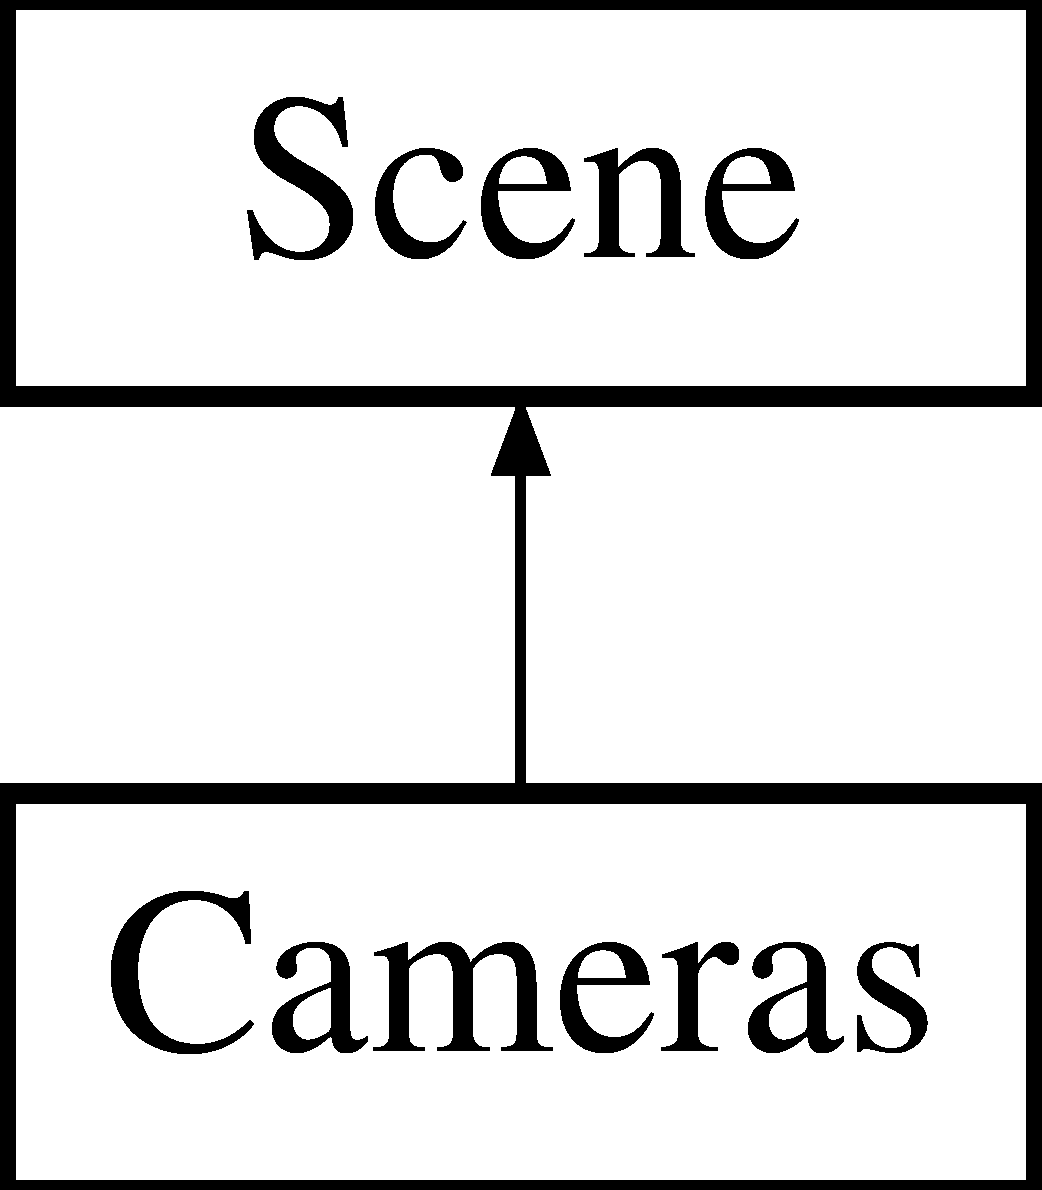
\includegraphics[height=2.000000cm]{class_cameras}
\end{center}
\end{figure}
\subsection*{Public Member Functions}
\begin{DoxyCompactItemize}
\item 
\hyperlink{class_cameras_a14342354c24f588c24e004a722849c3d}{Cameras} (void)
\begin{DoxyCompactList}\small\item\em Default constructor. \end{DoxyCompactList}\item 
\hyperlink{class_cameras_a7de763b562cce2a06cb120610987cd29}{$\sim$\-Cameras} (void)
\begin{DoxyCompactList}\small\item\em Default destructor. \end{DoxyCompactList}\item 
\hyperlink{class_camera}{Camera} $\ast$ \hyperlink{class_cameras_a436b481bf293ec6dfa09d2f89054c54b}{add\-Camera} (const std\-::string \&name)
\begin{DoxyCompactList}\small\item\em add\-Camera takes a name for a camera and returns a handle to a newly created camera. \end{DoxyCompactList}\item 
void \hyperlink{class_cameras_a9dee7bf1f2c56176c461fa2617ce4549}{pop\-Camera} (void)
\begin{DoxyCompactList}\small\item\em pop\-Camera removes the most recently added \hyperlink{class_camera}{Camera} from the scene. \end{DoxyCompactList}\item 
\hyperlink{class_camera}{Camera} $\ast$ \hyperlink{class_cameras_a971e1ffd27ff38d58f83996f87700e82}{next} (void)
\begin{DoxyCompactList}\small\item\em Sets the active camera to the next available one in the collection. \end{DoxyCompactList}\item 
\hyperlink{class_camera}{Camera} $\ast$ \hyperlink{class_cameras_a90eb5a3dda940ed494f592d094580dd8}{prev} (void)
\begin{DoxyCompactList}\small\item\em Sets the active \hyperlink{class_camera}{Camera} to the previous available one in the collection. \end{DoxyCompactList}\item 
\hyperlink{class_camera}{Camera} $\ast$ \hyperlink{class_cameras_a6002cbceb6a93092a1a029af486349a0}{active} (void) const 
\begin{DoxyCompactList}\small\item\em active returns the \hyperlink{class_camera}{Camera} in the collection that is considered 'active'. \end{DoxyCompactList}\item 
size\-\_\-t \hyperlink{class_cameras_acf7e92b5163efeeb88543e605d436a0e}{num\-Cameras} (void) const 
\begin{DoxyCompactList}\small\item\em num\-Cameras fetches the number of \hyperlink{class_cameras}{Cameras} in the collection. \end{DoxyCompactList}\item 
void \hyperlink{class_cameras_ac4fee80c5cd473ee4fa2360a95857da7}{idle\-Motion} (void)
\begin{DoxyCompactList}\small\item\em idle\-Motion calls the idle method on all child cameras. \end{DoxyCompactList}\item 
void \hyperlink{class_cameras_a0d0b08d599d471c0070665006f3bc437}{resize} (int width, int height)
\begin{DoxyCompactList}\small\item\em resize informs the \hyperlink{class_cameras}{Cameras} collection of the new window size. \end{DoxyCompactList}\item 
void \hyperlink{class_cameras_a9d3b24eec1504127e4942aa0e9412ae7}{calculate\-Viewports} (void)
\begin{DoxyCompactList}\small\item\em For each \hyperlink{class_camera}{Camera} in the collection, computes the position and size of that \hyperlink{class_camera}{Camera}'s viewport in a split-\/screen, single-\/window configuration. \end{DoxyCompactList}\item 
void \hyperlink{class_cameras_adeb29c1d639fcfbae4c68017bc8ef4d4}{view} (void($\ast$draw\-\_\-func)(void))
\begin{DoxyCompactList}\small\item\em view calls the view method on all child cameras, followed by the provided draw function. \end{DoxyCompactList}\item 
\hyperlink{class_camera}{Camera} $\ast$ \hyperlink{class_cameras_a8a6c7958396c6b0d07380aa762b15fcc}{obj2\-Cam} (std\-::list$<$ \hyperlink{class_object}{Object} $\ast$ $>$\-::iterator \&it)
\begin{DoxyCompactList}\small\item\em obj2\-Cam is a gross hack; the function is used as a utility to convert \hyperlink{class_object}{Object} pointers to \hyperlink{class_camera}{Camera} pointers safely. \end{DoxyCompactList}\item 
virtual void \hyperlink{class_scene_a3ea7e92935755c776c235a9872f53394}{shader} (G\-Luint g\-Shader)
\begin{DoxyCompactList}\small\item\em Sets the Default shader for the scene. \end{DoxyCompactList}\item 
G\-Luint \hyperlink{class_scene_a9d8a33f0f0a296aba0fb6717ab85cb18}{shader} (void)
\begin{DoxyCompactList}\small\item\em Retrieves the handle for the default shader for the scene. \end{DoxyCompactList}\item 
\hypertarget{class_scene_aa5a48614e959c38c35d824fa9d6a4b8b}{\hyperlink{class_object}{Object} $\ast$ {\bfseries add\-Object} (const std\-::string \&obj\-Name, G\-Luint Object\-\_\-\-Shader=0)}\label{class_scene_aa5a48614e959c38c35d824fa9d6a4b8b}

\item 
\hypertarget{class_scene_a2a6845dacbb468c5c097c7a6ab5a0fe0}{void {\bfseries del\-Object} (const std\-::string \&obj\-Name)}\label{class_scene_a2a6845dacbb468c5c097c7a6ab5a0fe0}

\item 
\hypertarget{class_scene_a2e6b319b60e27e66ad43bb942a6c4424}{void {\bfseries del\-Object} (void)}\label{class_scene_a2e6b319b60e27e66ad43bb942a6c4424}

\item 
\hypertarget{class_scene_ad6c9d1d1d0c786d39bf97dc60410e28b}{void {\bfseries pop\-Object} (void)}\label{class_scene_ad6c9d1d1d0c786d39bf97dc60410e28b}

\item 
\hypertarget{class_scene_a8c57e1cebc39586c7928225d1e25de39}{void \hyperlink{class_scene_a8c57e1cebc39586c7928225d1e25de39}{destroy\-Object} (void)}\label{class_scene_a8c57e1cebc39586c7928225d1e25de39}

\begin{DoxyCompactList}\small\item\em Completely remove this object and all his children. \end{DoxyCompactList}\item 
\hypertarget{class_scene_a41fbbe388ea322df338648e66611ffcf}{void {\bfseries draw} (void)}\label{class_scene_a41fbbe388ea322df338648e66611ffcf}

\item 
\hypertarget{class_scene_ae9b69d8db8a46991017635f22e45baad}{\hyperlink{class_object}{Object} $\ast$ {\bfseries operator\mbox{[}$\,$\mbox{]}} (const std\-::string \&objname)}\label{class_scene_ae9b69d8db8a46991017635f22e45baad}

\end{DoxyCompactItemize}
\subsection*{Protected Member Functions}
\begin{DoxyCompactItemize}
\item 
void \hyperlink{class_scene_ad3897f8ac658af62c133783b2c4eaee4}{delete\-Object} (\hyperlink{class_object}{Object} $\ast$obj)
\begin{DoxyCompactList}\small\item\em delete\-Object is the actual implementation function that will remove an \hyperlink{class_object}{Object} from the \hyperlink{class_scene}{Scene} list and \hyperlink{class_scene}{Scene} map, then free the object. \end{DoxyCompactList}\item 
\hypertarget{class_scene_ab64354bd8059bab589ca2dbf9de9e66c}{void {\bfseries insert\-Object} (const std\-::string name, \hyperlink{class_object}{Object} $\ast$obj)}\label{class_scene_ab64354bd8059bab589ca2dbf9de9e66c}

\end{DoxyCompactItemize}
\subsection*{Protected Attributes}
\begin{DoxyCompactItemize}
\item 
\hypertarget{class_scene_acdd0123ca6b2d64d8d447bb485b235fc}{std\-::list$<$ \hyperlink{class_object}{Object} $\ast$ $>$ {\bfseries \-\_\-list}}\label{class_scene_acdd0123ca6b2d64d8d447bb485b235fc}

\item 
\hypertarget{class_scene_a8bd5d86484a12255b26b92b6cbf8d29a}{std\-::map$<$ std\-::string, \hyperlink{class_object}{Object} $\ast$ $>$ {\bfseries \-\_\-map}}\label{class_scene_a8bd5d86484a12255b26b92b6cbf8d29a}

\item 
\hypertarget{class_scene_ae87ca5350fcc595f3f15a4fd3c39f3d9}{std\-::list$<$ \hyperlink{class_object}{Object} $\ast$ $>$\-::iterator {\bfseries \-\_\-current\-Obj}}\label{class_scene_ae87ca5350fcc595f3f15a4fd3c39f3d9}

\item 
\hypertarget{class_scene_a8f9bdd8ec5edb1f414fbd314a36e2724}{G\-Luint {\bfseries \-\_\-g\-Shader}}\label{class_scene_a8f9bdd8ec5edb1f414fbd314a36e2724}

\end{DoxyCompactItemize}
\subsection*{Private Attributes}
\begin{DoxyCompactItemize}
\item 
\hypertarget{class_cameras_a2c40cd131741e1904fdfb024006258fd}{\hyperlink{struct_angel_1_1vec2}{Angel\-::vec2} \hyperlink{class_cameras_a2c40cd131741e1904fdfb024006258fd}{\-\_\-size}}\label{class_cameras_a2c40cd131741e1904fdfb024006258fd}

\begin{DoxyCompactList}\small\item\em \-\_\-size is a simple vec2 (x,y) that contains the size of the screen. \end{DoxyCompactList}\end{DoxyCompactItemize}


\subsection{Detailed Description}
The \hyperlink{class_cameras}{Cameras} class represents a group of logical cameras for a model view. Each camera possesses its own current viewing angle, and an absolute position in space. 

\begin{DoxyAuthor}{Author}
John Huston, \href{mailto:jhuston@cs.uml.edu}{\tt jhuston@cs.\-uml.\-edu} 
\end{DoxyAuthor}
\begin{DoxySince}{Since}
28 Nov 2012
\end{DoxySince}
Each \hyperlink{class_camera}{Camera} possesses its own C\-T\-M which can be resent to the G\-P\-U at will. 

Definition at line 29 of file Cameras.\-hpp.



\subsection{Constructor \& Destructor Documentation}
\hypertarget{class_cameras_a14342354c24f588c24e004a722849c3d}{\index{Cameras@{Cameras}!Cameras@{Cameras}}
\index{Cameras@{Cameras}!Cameras@{Cameras}}
\subsubsection[{Cameras}]{\setlength{\rightskip}{0pt plus 5cm}Cameras\-::\-Cameras (
\begin{DoxyParamCaption}
\item[{void}]{}
\end{DoxyParamCaption}
)}}\label{class_cameras_a14342354c24f588c24e004a722849c3d}


Default constructor. 

Nothing special. 

Definition at line 19 of file Cameras.\-cpp.

\hypertarget{class_cameras_a7de763b562cce2a06cb120610987cd29}{\index{Cameras@{Cameras}!$\sim$\-Cameras@{$\sim$\-Cameras}}
\index{$\sim$\-Cameras@{$\sim$\-Cameras}!Cameras@{Cameras}}
\subsubsection[{$\sim$\-Cameras}]{\setlength{\rightskip}{0pt plus 5cm}Cameras\-::$\sim$\-Cameras (
\begin{DoxyParamCaption}
\item[{void}]{}
\end{DoxyParamCaption}
)}}\label{class_cameras_a7de763b562cce2a06cb120610987cd29}


Default destructor. 

Nothing special here, either. 

Definition at line 26 of file Cameras.\-cpp.



\subsection{Member Function Documentation}
\hypertarget{class_cameras_a6002cbceb6a93092a1a029af486349a0}{\index{Cameras@{Cameras}!active@{active}}
\index{active@{active}!Cameras@{Cameras}}
\subsubsection[{active}]{\setlength{\rightskip}{0pt plus 5cm}{\bf Camera} $\ast$ Cameras\-::active (
\begin{DoxyParamCaption}
\item[{void}]{}
\end{DoxyParamCaption}
) const}}\label{class_cameras_a6002cbceb6a93092a1a029af486349a0}


active returns the \hyperlink{class_camera}{Camera} in the collection that is considered 'active'. 

\begin{DoxyReturn}{Returns}
A pointer to the currently selected, active \hyperlink{class_camera}{Camera}. 
\end{DoxyReturn}


Definition at line 86 of file Cameras.\-cpp.

\hypertarget{class_cameras_a436b481bf293ec6dfa09d2f89054c54b}{\index{Cameras@{Cameras}!add\-Camera@{add\-Camera}}
\index{add\-Camera@{add\-Camera}!Cameras@{Cameras}}
\subsubsection[{add\-Camera}]{\setlength{\rightskip}{0pt plus 5cm}{\bf Camera} $\ast$ Cameras\-::add\-Camera (
\begin{DoxyParamCaption}
\item[{const std\-::string \&}]{name}
\end{DoxyParamCaption}
)}}\label{class_cameras_a436b481bf293ec6dfa09d2f89054c54b}


add\-Camera takes a name for a camera and returns a handle to a newly created camera. 


\begin{DoxyParams}{Parameters}
{\em name} & The name of the new camera to create. \\
\hline
\end{DoxyParams}
\begin{DoxyReturn}{Returns}
A Pointer to a newly created \hyperlink{class_camera}{Camera} object. 
\end{DoxyReturn}


Definition at line 35 of file Cameras.\-cpp.

\hypertarget{class_cameras_a9d3b24eec1504127e4942aa0e9412ae7}{\index{Cameras@{Cameras}!calculate\-Viewports@{calculate\-Viewports}}
\index{calculate\-Viewports@{calculate\-Viewports}!Cameras@{Cameras}}
\subsubsection[{calculate\-Viewports}]{\setlength{\rightskip}{0pt plus 5cm}void Cameras\-::calculate\-Viewports (
\begin{DoxyParamCaption}
\item[{void}]{}
\end{DoxyParamCaption}
)}}\label{class_cameras_a9d3b24eec1504127e4942aa0e9412ae7}


For each \hyperlink{class_camera}{Camera} in the collection, computes the position and size of that \hyperlink{class_camera}{Camera}'s viewport in a split-\/screen, single-\/window configuration. 

The \hyperlink{class_camera}{Camera} object is updated with the new information.

\begin{DoxyReturn}{Returns}
void.

void. 
\end{DoxyReturn}


Definition at line 141 of file Cameras.\-cpp.

\hypertarget{class_scene_ad3897f8ac658af62c133783b2c4eaee4}{\index{Cameras@{Cameras}!delete\-Object@{delete\-Object}}
\index{delete\-Object@{delete\-Object}!Cameras@{Cameras}}
\subsubsection[{delete\-Object}]{\setlength{\rightskip}{0pt plus 5cm}void Scene\-::delete\-Object (
\begin{DoxyParamCaption}
\item[{{\bf Object} $\ast$}]{obj}
\end{DoxyParamCaption}
)\hspace{0.3cm}{\ttfamily [protected]}, {\ttfamily [inherited]}}}\label{class_scene_ad3897f8ac658af62c133783b2c4eaee4}


delete\-Object is the actual implementation function that will remove an \hyperlink{class_object}{Object} from the \hyperlink{class_scene}{Scene} list and \hyperlink{class_scene}{Scene} map, then free the object. 


\begin{DoxyParams}{Parameters}
{\em obj} & The pointer to the object to free. \\
\hline
\end{DoxyParams}


Definition at line 76 of file Scene.\-cpp.

\hypertarget{class_cameras_ac4fee80c5cd473ee4fa2360a95857da7}{\index{Cameras@{Cameras}!idle\-Motion@{idle\-Motion}}
\index{idle\-Motion@{idle\-Motion}!Cameras@{Cameras}}
\subsubsection[{idle\-Motion}]{\setlength{\rightskip}{0pt plus 5cm}void Cameras\-::idle\-Motion (
\begin{DoxyParamCaption}
\item[{void}]{}
\end{DoxyParamCaption}
)}}\label{class_cameras_ac4fee80c5cd473ee4fa2360a95857da7}


idle\-Motion calls the idle method on all child cameras. 

Intended to be called during the \hyperlink{ds_8cpp_a01131b63acf241e9db91704d89ce15d2}{idle()} loop in G\-L\-U\-T.

\begin{DoxyReturn}{Returns}
void. 
\end{DoxyReturn}


Definition at line 111 of file Cameras.\-cpp.

\hypertarget{class_cameras_a971e1ffd27ff38d58f83996f87700e82}{\index{Cameras@{Cameras}!next@{next}}
\index{next@{next}!Cameras@{Cameras}}
\subsubsection[{next}]{\setlength{\rightskip}{0pt plus 5cm}{\bf Camera} $\ast$ Cameras\-::next (
\begin{DoxyParamCaption}
\item[{void}]{}
\end{DoxyParamCaption}
)}}\label{class_cameras_a971e1ffd27ff38d58f83996f87700e82}


Sets the active camera to the next available one in the collection. 

Sets the active \hyperlink{class_camera}{Camera} to the next available one in the collection.

\begin{DoxyReturn}{Returns}
A pointer to the newly active \hyperlink{class_camera}{Camera}. 
\end{DoxyReturn}


Definition at line 64 of file Cameras.\-cpp.

\hypertarget{class_cameras_acf7e92b5163efeeb88543e605d436a0e}{\index{Cameras@{Cameras}!num\-Cameras@{num\-Cameras}}
\index{num\-Cameras@{num\-Cameras}!Cameras@{Cameras}}
\subsubsection[{num\-Cameras}]{\setlength{\rightskip}{0pt plus 5cm}size\-\_\-t Cameras\-::num\-Cameras (
\begin{DoxyParamCaption}
\item[{void}]{}
\end{DoxyParamCaption}
) const}}\label{class_cameras_acf7e92b5163efeeb88543e605d436a0e}


num\-Cameras fetches the number of \hyperlink{class_cameras}{Cameras} in the collection. 

\begin{DoxyReturn}{Returns}
an unsigned integer, the number of \hyperlink{class_cameras}{Cameras} in the collection. 
\end{DoxyReturn}


Definition at line 101 of file Cameras.\-cpp.

\hypertarget{class_cameras_a8a6c7958396c6b0d07380aa762b15fcc}{\index{Cameras@{Cameras}!obj2\-Cam@{obj2\-Cam}}
\index{obj2\-Cam@{obj2\-Cam}!Cameras@{Cameras}}
\subsubsection[{obj2\-Cam}]{\setlength{\rightskip}{0pt plus 5cm}{\bf Camera} $\ast$ Cameras\-::obj2\-Cam (
\begin{DoxyParamCaption}
\item[{std\-::list$<$ {\bf Object} $\ast$ $>$\-::iterator \&}]{it}
\end{DoxyParamCaption}
)}}\label{class_cameras_a8a6c7958396c6b0d07380aa762b15fcc}


obj2\-Cam is a gross hack; the function is used as a utility to convert \hyperlink{class_object}{Object} pointers to \hyperlink{class_camera}{Camera} pointers safely. 

F\-I\-X\-M\-E\-: Refactor the inheritance here to make this less hacky.


\begin{DoxyParams}{Parameters}
{\em it} & A list$<$\-Object$\ast$$>$ iterator that points to the \hyperlink{class_object}{Object}.\\
\hline
\end{DoxyParams}
\begin{DoxyReturn}{Returns}
A pointer to a \hyperlink{class_camera}{Camera} object. 
\end{DoxyReturn}


Definition at line 249 of file Cameras.\-cpp.

\hypertarget{class_cameras_a9dee7bf1f2c56176c461fa2617ce4549}{\index{Cameras@{Cameras}!pop\-Camera@{pop\-Camera}}
\index{pop\-Camera@{pop\-Camera}!Cameras@{Cameras}}
\subsubsection[{pop\-Camera}]{\setlength{\rightskip}{0pt plus 5cm}void Cameras\-::pop\-Camera (
\begin{DoxyParamCaption}
\item[{void}]{}
\end{DoxyParamCaption}
)}}\label{class_cameras_a9dee7bf1f2c56176c461fa2617ce4549}


pop\-Camera removes the most recently added \hyperlink{class_camera}{Camera} from the scene. 

\begin{DoxyReturn}{Returns}
void. 
\end{DoxyReturn}


Definition at line 50 of file Cameras.\-cpp.

\hypertarget{class_cameras_a90eb5a3dda940ed494f592d094580dd8}{\index{Cameras@{Cameras}!prev@{prev}}
\index{prev@{prev}!Cameras@{Cameras}}
\subsubsection[{prev}]{\setlength{\rightskip}{0pt plus 5cm}{\bf Camera} $\ast$ Cameras\-::prev (
\begin{DoxyParamCaption}
\item[{void}]{}
\end{DoxyParamCaption}
)}}\label{class_cameras_a90eb5a3dda940ed494f592d094580dd8}


Sets the active \hyperlink{class_camera}{Camera} to the previous available one in the collection. 

\begin{DoxyReturn}{Returns}
A pointer to the newly active \hyperlink{class_camera}{Camera}. 
\end{DoxyReturn}


Definition at line 75 of file Cameras.\-cpp.

\hypertarget{class_cameras_a0d0b08d599d471c0070665006f3bc437}{\index{Cameras@{Cameras}!resize@{resize}}
\index{resize@{resize}!Cameras@{Cameras}}
\subsubsection[{resize}]{\setlength{\rightskip}{0pt plus 5cm}void Cameras\-::resize (
\begin{DoxyParamCaption}
\item[{int}]{width, }
\item[{int}]{height}
\end{DoxyParamCaption}
)}}\label{class_cameras_a0d0b08d599d471c0070665006f3bc437}


resize informs the \hyperlink{class_cameras}{Cameras} collection of the new window size. 

Intended to be called from the G\-L\-U\-T main loop. This method also invokes \hyperlink{class_cameras_a9d3b24eec1504127e4942aa0e9412ae7}{Cameras\-::calculate\-Viewports}.


\begin{DoxyParams}{Parameters}
{\em width} & The new window width. \\
\hline
{\em height} & The new window height.\\
\hline
\end{DoxyParams}
\begin{DoxyReturn}{Returns}
void. 
\end{DoxyReturn}


Definition at line 128 of file Cameras.\-cpp.

\hypertarget{class_scene_a3ea7e92935755c776c235a9872f53394}{\index{Cameras@{Cameras}!shader@{shader}}
\index{shader@{shader}!Cameras@{Cameras}}
\subsubsection[{shader}]{\setlength{\rightskip}{0pt plus 5cm}void Scene\-::shader (
\begin{DoxyParamCaption}
\item[{G\-Luint}]{g\-Shader}
\end{DoxyParamCaption}
)\hspace{0.3cm}{\ttfamily [virtual]}, {\ttfamily [inherited]}}}\label{class_scene_a3ea7e92935755c776c235a9872f53394}


Sets the Default shader for the scene. 

In the context of inheritance by objects, This sets the shader to use to render the physical object.


\begin{DoxyParams}{Parameters}
{\em g\-Shader} & The G\-Luint handle to the shader to use.\\
\hline
\end{DoxyParams}
\begin{DoxyReturn}{Returns}
void. 
\end{DoxyReturn}


Reimplemented in \hyperlink{class_object_aeaf11bb87bd59381c9e066f0b4f40d8e}{Object}.



Definition at line 54 of file Scene.\-cpp.

\hypertarget{class_scene_a9d8a33f0f0a296aba0fb6717ab85cb18}{\index{Cameras@{Cameras}!shader@{shader}}
\index{shader@{shader}!Cameras@{Cameras}}
\subsubsection[{shader}]{\setlength{\rightskip}{0pt plus 5cm}G\-Luint Scene\-::shader (
\begin{DoxyParamCaption}
\item[{void}]{}
\end{DoxyParamCaption}
)\hspace{0.3cm}{\ttfamily [inherited]}}}\label{class_scene_a9d8a33f0f0a296aba0fb6717ab85cb18}


Retrieves the handle for the default shader for the scene. 

In the context of inheritance by objects, This retrieves the shader handle to use to draw the object.

\begin{DoxyReturn}{Returns}
A G\-Luint handle to the shader program. 
\end{DoxyReturn}


Definition at line 66 of file Scene.\-cpp.

\hypertarget{class_cameras_adeb29c1d639fcfbae4c68017bc8ef4d4}{\index{Cameras@{Cameras}!view@{view}}
\index{view@{view}!Cameras@{Cameras}}
\subsubsection[{view}]{\setlength{\rightskip}{0pt plus 5cm}void Cameras\-::view (
\begin{DoxyParamCaption}
\item[{void($\ast$)(void)}]{draw\-\_\-func}
\end{DoxyParamCaption}
)}}\label{class_cameras_adeb29c1d639fcfbae4c68017bc8ef4d4}


view calls the view method on all child cameras, followed by the provided draw function. 

Intended to be called during the \hyperlink{ds_8cpp_a4ea013001a5fb47853d0fab8f8de35cd}{display()} portion of the G\-L\-U\-T main loop.

\hyperlink{class_cameras_adeb29c1d639fcfbae4c68017bc8ef4d4}{view()} is intended to \char`\"{}set up\char`\"{} the object, but not actually draw it.


\begin{DoxyParams}{Parameters}
{\em draw\-\_\-func} & A pointer to a function that will actually draw the object. \\
\hline
\end{DoxyParams}


Definition at line 232 of file Cameras.\-cpp.



The documentation for this class was generated from the following files\-:\begin{DoxyCompactItemize}
\item 
\hyperlink{_cameras_8hpp}{Cameras.\-hpp}\item 
\hyperlink{_cameras_8cpp}{Cameras.\-cpp}\end{DoxyCompactItemize}

\input{class_engine}
\hypertarget{class_tiem_spelchk_1_1_lurn2_spiel_nub}{\section{Tiem\-Spelchk\-:\-:Lurn2\-Spiel\-Nub Class Reference}
\label{class_tiem_spelchk_1_1_lurn2_spiel_nub}\index{Tiem\-Spelchk\-::\-Lurn2\-Spiel\-Nub@{Tiem\-Spelchk\-::\-Lurn2\-Spiel\-Nub}}
}
\subsection*{Public Member Functions}
\begin{DoxyCompactItemize}
\item 
\hypertarget{class_tiem_spelchk_1_1_lurn2_spiel_nub_a590dbbc3cfd3781cc79e63945d6bdce9}{void {\bfseries set\-Callback} (boost\-::function$<$ void(int, double, double, double) $>$ head\-C\-B)}\label{class_tiem_spelchk_1_1_lurn2_spiel_nub_a590dbbc3cfd3781cc79e63945d6bdce9}

\item 
\hypertarget{class_tiem_spelchk_1_1_lurn2_spiel_nub_a29b93d8ad5bbcefad6df00b4a23f4fc4}{int {\bfseries Start} ()}\label{class_tiem_spelchk_1_1_lurn2_spiel_nub_a29b93d8ad5bbcefad6df00b4a23f4fc4}

\item 
\hypertarget{class_tiem_spelchk_1_1_lurn2_spiel_nub_a7c055489ec5c140e7bfa91a0c0a76f94}{void {\bfseries Shutdown} ()}\label{class_tiem_spelchk_1_1_lurn2_spiel_nub_a7c055489ec5c140e7bfa91a0c0a76f94}

\end{DoxyCompactItemize}
\subsection*{Static Public Member Functions}
\begin{DoxyCompactItemize}
\item 
\hypertarget{class_tiem_spelchk_1_1_lurn2_spiel_nub_a38db742a870fe48644f795c3e249d6ab}{static void X\-N\-\_\-\-C\-A\-L\-L\-B\-A\-C\-K\-\_\-\-T\-Y\-P\-E {\bfseries new\-\_\-user} (xn\-::\-User\-Generator \&, Xn\-User\-I\-D, void $\ast$)}\label{class_tiem_spelchk_1_1_lurn2_spiel_nub_a38db742a870fe48644f795c3e249d6ab}

\item 
\hypertarget{class_tiem_spelchk_1_1_lurn2_spiel_nub_a9d85ee4de4621c0de0c7133fb15bcaa6}{static void X\-N\-\_\-\-C\-A\-L\-L\-B\-A\-C\-K\-\_\-\-T\-Y\-P\-E {\bfseries lost\-\_\-user} (xn\-::\-User\-Generator \&, Xn\-User\-I\-D, void $\ast$)}\label{class_tiem_spelchk_1_1_lurn2_spiel_nub_a9d85ee4de4621c0de0c7133fb15bcaa6}

\item 
\hypertarget{class_tiem_spelchk_1_1_lurn2_spiel_nub_a9e8df7c3c86b521fd642e6bd1719b1ad}{static void X\-N\-\_\-\-C\-A\-L\-L\-B\-A\-C\-K\-\_\-\-T\-Y\-P\-E {\bfseries pose} (xn\-::\-Pose\-Detection\-Capability \&, const Xn\-Char $\ast$, Xn\-User\-I\-D, void $\ast$)}\label{class_tiem_spelchk_1_1_lurn2_spiel_nub_a9e8df7c3c86b521fd642e6bd1719b1ad}

\item 
\hypertarget{class_tiem_spelchk_1_1_lurn2_spiel_nub_aeb00f8d55630f3f7d2da36d04302a174}{static void X\-N\-\_\-\-C\-A\-L\-L\-B\-A\-C\-K\-\_\-\-T\-Y\-P\-E {\bfseries cal\-\_\-start} (xn\-::\-Skeleton\-Capability \&, Xn\-User\-I\-D, void $\ast$)}\label{class_tiem_spelchk_1_1_lurn2_spiel_nub_aeb00f8d55630f3f7d2da36d04302a174}

\item 
\hypertarget{class_tiem_spelchk_1_1_lurn2_spiel_nub_a41dd33b54013b3974119d7a0da893d8a}{static void X\-N\-\_\-\-C\-A\-L\-L\-B\-A\-C\-K\-\_\-\-T\-Y\-P\-E {\bfseries cal\-\_\-complete} (xn\-::\-Skeleton\-Capability \&, Xn\-User\-I\-D, Xn\-Calibration\-Status, void $\ast$)}\label{class_tiem_spelchk_1_1_lurn2_spiel_nub_a41dd33b54013b3974119d7a0da893d8a}

\end{DoxyCompactItemize}
\subsection*{Private Member Functions}
\begin{DoxyCompactItemize}
\item 
\hypertarget{class_tiem_spelchk_1_1_lurn2_spiel_nub_a28fa0e11dc89f2202890ec873a74d23f}{void {\bfseries F\-U\-N\-K\-M\-A\-S\-T\-E\-R\-\_\-thread\-\_\-func} ()}\label{class_tiem_spelchk_1_1_lurn2_spiel_nub_a28fa0e11dc89f2202890ec873a74d23f}

\item 
\hypertarget{class_tiem_spelchk_1_1_lurn2_spiel_nub_aa28206499ebeb98e2db24db9813232f7}{void X\-N\-\_\-\-C\-A\-L\-L\-B\-A\-C\-K\-\_\-\-T\-Y\-P\-E {\bfseries User\-\_\-\-New\-User} (xn\-::\-User\-Generator \&, Xn\-User\-I\-D n\-Id, void $\ast$)}\label{class_tiem_spelchk_1_1_lurn2_spiel_nub_aa28206499ebeb98e2db24db9813232f7}

\item 
\hypertarget{class_tiem_spelchk_1_1_lurn2_spiel_nub_a040124fb9e20cfab39c45d334e6c5b1c}{void X\-N\-\_\-\-C\-A\-L\-L\-B\-A\-C\-K\-\_\-\-T\-Y\-P\-E {\bfseries User\-\_\-\-Lost\-User} (xn\-::\-User\-Generator \&, Xn\-User\-I\-D n\-Id, void $\ast$)}\label{class_tiem_spelchk_1_1_lurn2_spiel_nub_a040124fb9e20cfab39c45d334e6c5b1c}

\item 
\hypertarget{class_tiem_spelchk_1_1_lurn2_spiel_nub_a5bc3222dbbbee803b2b77afbdbd88acc}{void X\-N\-\_\-\-C\-A\-L\-L\-B\-A\-C\-K\-\_\-\-T\-Y\-P\-E {\bfseries User\-Pose\-\_\-\-Pose\-Detected} (xn\-::\-Pose\-Detection\-Capability \&, const Xn\-Char $\ast$str\-Pose, Xn\-User\-I\-D n\-Id, void $\ast$)}\label{class_tiem_spelchk_1_1_lurn2_spiel_nub_a5bc3222dbbbee803b2b77afbdbd88acc}

\item 
\hypertarget{class_tiem_spelchk_1_1_lurn2_spiel_nub_aaf9264a46a4b2c23587fc67569339992}{void X\-N\-\_\-\-C\-A\-L\-L\-B\-A\-C\-K\-\_\-\-T\-Y\-P\-E {\bfseries User\-Calibration\-\_\-\-Calibration\-Start} (xn\-::\-Skeleton\-Capability \&, Xn\-User\-I\-D n\-Id, void $\ast$)}\label{class_tiem_spelchk_1_1_lurn2_spiel_nub_aaf9264a46a4b2c23587fc67569339992}

\item 
\hypertarget{class_tiem_spelchk_1_1_lurn2_spiel_nub_ad029dba23118fdb5fa2b2cfc74a50305}{void X\-N\-\_\-\-C\-A\-L\-L\-B\-A\-C\-K\-\_\-\-T\-Y\-P\-E {\bfseries User\-Calibration\-\_\-\-Calibration\-Complete} (xn\-::\-Skeleton\-Capability \&, Xn\-User\-I\-D n\-Id, Xn\-Calibration\-Status e\-Status, void $\ast$)}\label{class_tiem_spelchk_1_1_lurn2_spiel_nub_ad029dba23118fdb5fa2b2cfc74a50305}

\end{DoxyCompactItemize}
\subsection*{Private Attributes}
\begin{DoxyCompactItemize}
\item 
\hypertarget{class_tiem_spelchk_1_1_lurn2_spiel_nub_a46cded6cb265dfcd1c73393952ab0529}{boost\-::function$<$ void(int, \\*
double, double, double) $>$ {\bfseries \-\_\-cb}}\label{class_tiem_spelchk_1_1_lurn2_spiel_nub_a46cded6cb265dfcd1c73393952ab0529}

\item 
\hypertarget{class_tiem_spelchk_1_1_lurn2_spiel_nub_a6ce714e2ff4d16b836a16ac526b397fe}{boost\-::thread {\bfseries \-\_\-thread}}\label{class_tiem_spelchk_1_1_lurn2_spiel_nub_a6ce714e2ff4d16b836a16ac526b397fe}

\item 
\hypertarget{class_tiem_spelchk_1_1_lurn2_spiel_nub_ab0b7fd2f68507a79f940ece0c7ce2cb6}{bool {\bfseries needs\-To\-Seppuku}}\label{class_tiem_spelchk_1_1_lurn2_spiel_nub_ab0b7fd2f68507a79f940ece0c7ce2cb6}

\item 
\hypertarget{class_tiem_spelchk_1_1_lurn2_spiel_nub_a89dc8acb0e9b63f52de20364f5c49c47}{xn\-::\-Context {\bfseries g\-\_\-\-Context}}\label{class_tiem_spelchk_1_1_lurn2_spiel_nub_a89dc8acb0e9b63f52de20364f5c49c47}

\item 
\hypertarget{class_tiem_spelchk_1_1_lurn2_spiel_nub_a2500c966681a65ffcd3d2354848227e5}{xn\-::\-Script\-Node {\bfseries g\-\_\-script\-Node}}\label{class_tiem_spelchk_1_1_lurn2_spiel_nub_a2500c966681a65ffcd3d2354848227e5}

\item 
\hypertarget{class_tiem_spelchk_1_1_lurn2_spiel_nub_a7e4f74ecd9de1cfdff8cc2d237ce6e34}{xn\-::\-Depth\-Generator {\bfseries g\-\_\-\-Depth\-Generator}}\label{class_tiem_spelchk_1_1_lurn2_spiel_nub_a7e4f74ecd9de1cfdff8cc2d237ce6e34}

\item 
\hypertarget{class_tiem_spelchk_1_1_lurn2_spiel_nub_ad76a0650fa08d75e692125f3e2e571d0}{xn\-::\-User\-Generator {\bfseries g\-\_\-\-User\-Generator}}\label{class_tiem_spelchk_1_1_lurn2_spiel_nub_ad76a0650fa08d75e692125f3e2e571d0}

\item 
\hypertarget{class_tiem_spelchk_1_1_lurn2_spiel_nub_a3d0fa17772cdaa4775c6eb3c441f1b17}{Xn\-Bool {\bfseries g\-\_\-b\-Need\-Pose}}\label{class_tiem_spelchk_1_1_lurn2_spiel_nub_a3d0fa17772cdaa4775c6eb3c441f1b17}

\item 
\hypertarget{class_tiem_spelchk_1_1_lurn2_spiel_nub_ac2be8464e1436a7f90e2212e31944b7a}{Xn\-Char {\bfseries g\-\_\-str\-Pose} \mbox{[}20\mbox{]}}\label{class_tiem_spelchk_1_1_lurn2_spiel_nub_ac2be8464e1436a7f90e2212e31944b7a}

\end{DoxyCompactItemize}


\subsection{Detailed Description}


Definition at line 56 of file Kinect\-Inator.\-hpp.



The documentation for this class was generated from the following files\-:\begin{DoxyCompactItemize}
\item 
\hyperlink{_kinect_inator_8hpp}{Kinect\-Inator.\-hpp}\item 
\hyperlink{_kinect_inator_8cpp}{Kinect\-Inator.\-cpp}\end{DoxyCompactItemize}

\input{class_angel_1_1mat2}
\input{class_angel_1_1mat3}
\input{class_angel_1_1mat4}
\hypertarget{class_object}{\section{Object Class Reference}
\label{class_object}\index{Object@{Object}}
}


\hyperlink{class_object}{Object} Class\-: Renderable \hyperlink{class_object}{Object} Implementation.  




{\ttfamily \#include $<$Object.\-hpp$>$}

Inheritance diagram for Object\-:\begin{figure}[H]
\begin{center}
\leavevmode
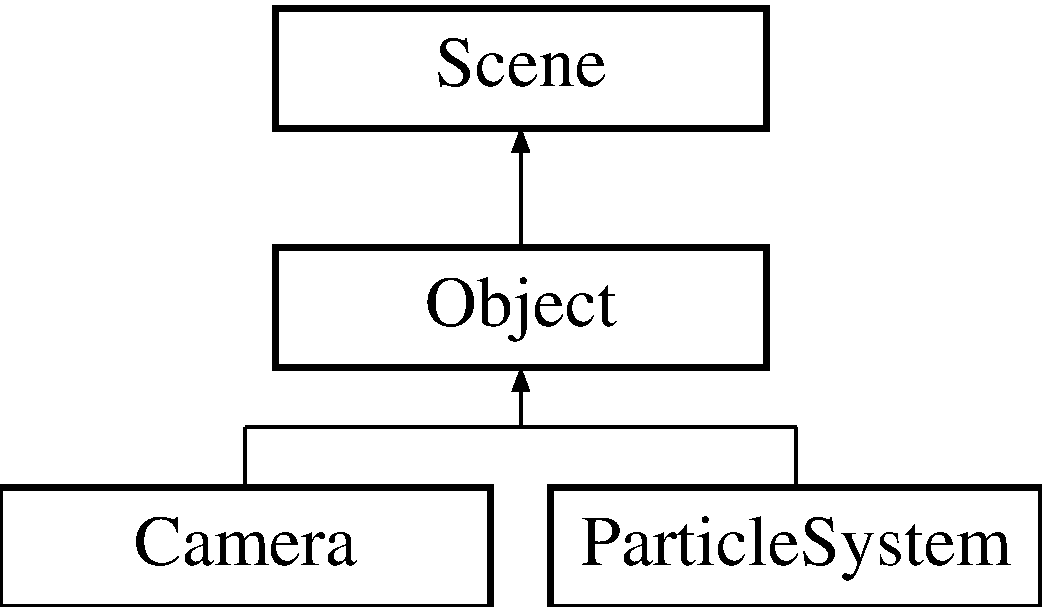
\includegraphics[height=3.000000cm]{class_object}
\end{center}
\end{figure}
\subsection*{Public Types}
\begin{DoxyCompactItemize}
\item 
enum \hyperlink{class_object_a8c11d8700b0bb79a46c61f2de4f23fa3}{Uniforms} \{ \\*
\hyperlink{class_object_a8c11d8700b0bb79a46c61f2de4f23fa3a8a65225741e4db1df295c9cab71a98c0}{B\-E\-G\-I\-N}, 
\hyperlink{class_object_a8c11d8700b0bb79a46c61f2de4f23fa3a8fecaee23530c9befe7feb5166e81484}{I\-S\-\_\-\-T\-E\-X\-T\-U\-R\-E\-D} =  B\-E\-G\-I\-N, 
\hyperlink{class_object_a8c11d8700b0bb79a46c61f2de4f23fa3a9aaf45d5144b52065016b5b39e909851}{O\-B\-J\-E\-C\-T\-\_\-\-C\-T\-M}, 
\hyperlink{class_object_a8c11d8700b0bb79a46c61f2de4f23fa3ac93e286d52dad730ccf3fdab9b102902}{M\-O\-R\-P\-H\-\_\-\-P\-C\-T}, 
\\*
\hyperlink{class_object_a8c11d8700b0bb79a46c61f2de4f23fa3a85f87adc3e3d4242733729ee87b21423}{T\-E\-X\-\_\-\-S\-A\-M\-P\-L\-E\-R}, 
\hyperlink{class_object_a8c11d8700b0bb79a46c61f2de4f23fa3ad78facbf844c1259f464a49061e1d7ed}{E\-N\-D}
 \}
\begin{DoxyCompactList}\small\item\em enum Uniforms describes the properties of the base object that need to be visible to the G\-P\-U. \end{DoxyCompactList}\item 
typedef const unsigned int \hyperlink{class_object_a79b74057dbc5182b85c9c3ba8480fcf2}{Uniform\-Enum}
\begin{DoxyCompactList}\small\item\em The \hyperlink{class_object}{Object} class takes advantage of child-\/extendible enumerations. \end{DoxyCompactList}\item 
typedef std\-::map\\*
$<$ \hyperlink{class_object_a79b74057dbc5182b85c9c3ba8480fcf2}{Object\-::\-Uniform\-Enum}, \\*
std\-::string $>$ \hyperlink{class_object_a6e19bd8516360bff956408cbae33b878}{Uniform\-Map}
\begin{DoxyCompactList}\small\item\em We store mappings of Uniform Enumerations, The desired function of the var, to strings, the names of the variables. \end{DoxyCompactList}\item 
typedef enum \hyperlink{class_object_a8c11d8700b0bb79a46c61f2de4f23fa3}{Object\-::\-Uniforms} \hyperlink{class_object_ae6a2969ddca87d2c54b7cb1c131a7d60}{Uniform}
\begin{DoxyCompactList}\small\item\em enum Uniforms describes the properties of the base object that need to be visible to the G\-P\-U. \end{DoxyCompactList}\end{DoxyCompactItemize}
\subsection*{Public Member Functions}
\begin{DoxyCompactItemize}
\item 
\hyperlink{class_object_aacf42e81415f32f1f2a105ce29c7c1b9}{Object} (const std\-::string \&\hyperlink{class_object_aafd766fce2598f718cac97a3ac731706}{name}, G\-Luint g\-Shader)
\begin{DoxyCompactList}\small\item\em Constructor. \end{DoxyCompactList}\item 
\hypertarget{class_object_ac9ec2177266554587e8ddb40eb72ae1c}{virtual \hyperlink{class_object_ac9ec2177266554587e8ddb40eb72ae1c}{$\sim$\-Object} (void)}\label{class_object_ac9ec2177266554587e8ddb40eb72ae1c}

\begin{DoxyCompactList}\small\item\em Default destructor. \end{DoxyCompactList}\item 
\hypertarget{class_object_a53e2ee7f548550be014126bed139fe69}{void \hyperlink{class_object_a53e2ee7f548550be014126bed139fe69}{draw} (void)}\label{class_object_a53e2ee7f548550be014126bed139fe69}

\begin{DoxyCompactList}\small\item\em draw method\-: Render this object to the screen \-\_\-buffer. \end{DoxyCompactList}\item 
\hypertarget{class_object_a7edb92c30d86b6479b0ff2a5e9f06e13}{void \hyperlink{class_object_a7edb92c30d86b6479b0ff2a5e9f06e13}{buffer} (void)}\label{class_object_a7edb92c30d86b6479b0ff2a5e9f06e13}

\begin{DoxyCompactList}\small\item\em buffer all of our data\-: Vertices, Tex\-U\-Vs, Normals, Indices, Colors and Morph Buffers. \end{DoxyCompactList}\item 
\hypertarget{class_object_a293792abfe0671e00a0ec10e85ea9d9e}{void \hyperlink{class_object_a293792abfe0671e00a0ec10e85ea9d9e}{buffer\-Morph\-Only} (void)}\label{class_object_a293792abfe0671e00a0ec10e85ea9d9e}

\begin{DoxyCompactList}\small\item\em buffer only the Morph-\/related buffers. \end{DoxyCompactList}\item 
void \hyperlink{class_object_adafdf22583b051b4c61c8eb725fb07d5}{draw\-Mode} (G\-Lenum new\-\_\-mode)
\begin{DoxyCompactList}\small\item\em Select a new Open\-G\-L draw mode for this \hyperlink{class_object}{Object}. \end{DoxyCompactList}\item 
void \hyperlink{class_object_afebb27ddb10daed8e2c5085b76cbc500}{texture} (const char $\ast$$\ast$filename)
\begin{DoxyCompactList}\small\item\em F\-I\-X\-M\-E\-: This is a junk, nonflexible method. \end{DoxyCompactList}\item 
const std\-::string \& \hyperlink{class_object_aafd766fce2598f718cac97a3ac731706}{name} (void) const 
\begin{DoxyCompactList}\small\item\em Retrieve the \-\_\-name of this \hyperlink{class_object}{Object}. \end{DoxyCompactList}\item 
virtual void \hyperlink{class_object_a11d6063c580331d6af59c8d71b7f3e9f}{link} (\hyperlink{class_object_a79b74057dbc5182b85c9c3ba8480fcf2}{Uniform\-Enum} which, const std\-::string \&\hyperlink{class_object_aafd766fce2598f718cac97a3ac731706}{name})
\begin{DoxyCompactList}\small\item\em link a specified Uniform against the shader's variable \-\_\-name. \end{DoxyCompactList}\item 
virtual void \hyperlink{class_object_a34258ee199342d785c29d18c49d54e71}{send} (\hyperlink{class_object_a79b74057dbc5182b85c9c3ba8480fcf2}{Uniform\-Enum} which)
\begin{DoxyCompactList}\small\item\em Send a Uniform to the shader. \end{DoxyCompactList}\item 
virtual G\-Luint \hyperlink{class_object_a459489106838a1e3a8dbbd13045cd523}{shader} (void)
\begin{DoxyCompactList}\small\item\em Returns the \hyperlink{class_object}{Object}'s current shader. \end{DoxyCompactList}\item 
virtual void \hyperlink{class_object_aeaf11bb87bd59381c9e066f0b4f40d8e}{shader} (G\-Luint new\-Shader)
\begin{DoxyCompactList}\small\item\em Sets the shader to be used by this object. \end{DoxyCompactList}\item 
void \hyperlink{class_object_a0d604a816115c474b9593aeaebda9f8b}{animation} (void($\ast$anim\-\_\-func)(\hyperlink{class_trans_cache}{Trans\-Cache} \&arg))
\begin{DoxyCompactList}\small\item\em Apply an animation callback function to this \hyperlink{class_object}{Object}. \end{DoxyCompactList}\item 
void \hyperlink{class_object_a2fdd201413e0408f5a2508874acd2ef5}{propagate} (void)
\begin{DoxyCompactList}\small\item\em Scene-\/graph changes are not automatically applied to children. \end{DoxyCompactList}\item 
\hyperlink{struct_angel_1_1vec4}{vec4} \hyperlink{class_object_ac64609eb614aa5974b74000cec6fc95c}{position} () const 
\begin{DoxyCompactList}\small\item\em Obtain the vec4 representative of the \hyperlink{class_object}{Object}'s current position in space. \end{DoxyCompactList}\item 
\hyperlink{class_object}{Object} $\ast$ \hyperlink{class_object_a7694c9cfe445c3d5b993a38e3f8badd9}{morph\-Target} () const 
\begin{DoxyCompactList}\small\item\em Retrieve a pointer to this object's morph target. \end{DoxyCompactList}\item 
\hyperlink{class_object}{Object} $\ast$ \hyperlink{class_object_ab0ba603904f8f7de15dc0450e2d9b30e}{gen\-Morph\-Target} (G\-Luint \hyperlink{class_object_a459489106838a1e3a8dbbd13045cd523}{shader})
\begin{DoxyCompactList}\small\item\em Instantiate a new morphing target. \end{DoxyCompactList}\item 
float \hyperlink{class_object_accb051cdc79bc93e8c9c0edb79dd6b30}{morph\-Percentage} () const 
\begin{DoxyCompactList}\small\item\em Retrieve the morph Percentage of this object. \end{DoxyCompactList}\item 
void \hyperlink{class_object_a543d2329b25df9fb0a782f09d03e5cb1}{morph\-Percentage} (const float new\-Percentage)
\begin{DoxyCompactList}\small\item\em Set the morph percentage of this \hyperlink{class_object}{Object}. \end{DoxyCompactList}\item 
\hypertarget{class_object_a98d3f1b9ebb61c3b21e2a59ed267480a}{void \hyperlink{class_object_a98d3f1b9ebb61c3b21e2a59ed267480a}{destroy\-Morph\-Target} ()}\label{class_object_a98d3f1b9ebb61c3b21e2a59ed267480a}

\begin{DoxyCompactList}\small\item\em Obliterate the morph target for this object. \end{DoxyCompactList}\item 
int \hyperlink{class_object_a73f1a6210bacf504de9a808009479b81}{number\-Of\-Points} ()
\begin{DoxyCompactList}\small\item\em Retrieve the number of \-\_\-vertices this object has. \end{DoxyCompactList}\item 
void \hyperlink{class_object_a74300b3fa318786e21b65183461c5e25}{texture\-I\-D} (G\-Lint new\-Texture\-I\-D)
\begin{DoxyCompactList}\small\item\em Set the \hyperlink{class_texture}{Texture} I\-D / \hyperlink{class_texture}{Texture} Unit for this \hyperlink{class_object}{Object}. \end{DoxyCompactList}\item 
\hyperlink{class_object}{Object} $\ast$ \hyperlink{class_scene_aa5a48614e959c38c35d824fa9d6a4b8b}{add\-Object} (const std\-::string \&obj\-Name, G\-Luint Object\-\_\-\-Shader=0)
\begin{DoxyCompactList}\small\item\em add\-Object creates a new \hyperlink{class_object}{Object} with the given name and, optionally, a specified shader and adds it to the \hyperlink{class_scene}{Scene} graph. \end{DoxyCompactList}\item 
void \hyperlink{class_scene_a2a6845dacbb468c5c097c7a6ab5a0fe0}{del\-Object} (const std\-::string \&obj\-Name)
\begin{DoxyCompactList}\small\item\em del\-Object will remove from the \hyperlink{class_scene}{Scene} graph the object with the given name. \end{DoxyCompactList}\item 
\hypertarget{class_scene_a2e6b319b60e27e66ad43bb942a6c4424}{void \hyperlink{class_scene_a2e6b319b60e27e66ad43bb942a6c4424}{del\-Object} (void)}\label{class_scene_a2e6b319b60e27e66ad43bb942a6c4424}

\begin{DoxyCompactList}\small\item\em del\-Object with no parameters will delete the first \hyperlink{class_object}{Object} in the \hyperlink{class_scene}{Scene}. \end{DoxyCompactList}\item 
\hypertarget{class_scene_ad6c9d1d1d0c786d39bf97dc60410e28b}{void \hyperlink{class_scene_ad6c9d1d1d0c786d39bf97dc60410e28b}{pop\-Object} (void)}\label{class_scene_ad6c9d1d1d0c786d39bf97dc60410e28b}

\begin{DoxyCompactList}\small\item\em pop\-Object deletes the last \hyperlink{class_object}{Object} in the \hyperlink{class_scene}{Scene}. \end{DoxyCompactList}\item 
\hypertarget{class_scene_a70fcdad192a4c6ff508125de8af6cf4d}{\hyperlink{class_object}{Object} $\ast$ {\bfseries next} (void)}\label{class_scene_a70fcdad192a4c6ff508125de8af6cf4d}

\item 
\hypertarget{class_scene_ac852d5d763eb35b4908c9aa7ea54d1ae}{\hyperlink{class_object}{Object} $\ast$ {\bfseries prev} (void)}\label{class_scene_ac852d5d763eb35b4908c9aa7ea54d1ae}

\item 
\hypertarget{class_scene_ad0ea1a6bcf7815c63988bd937f06eb23}{\hyperlink{class_object}{Object} $\ast$ {\bfseries active} (void) const }\label{class_scene_ad0ea1a6bcf7815c63988bd937f06eb23}

\item 
\hypertarget{class_scene_ae9b69d8db8a46991017635f22e45baad}{\hyperlink{class_object}{Object} $\ast$ {\bfseries operator\mbox{[}$\,$\mbox{]}} (const std\-::string \&objname)}\label{class_scene_ae9b69d8db8a46991017635f22e45baad}

\item 
void \hyperlink{class_scene_a8893899f0088a72642ae32a656252e7f}{insert\-Object} (\hyperlink{class_object}{Object} $\ast$obj)
\begin{DoxyCompactList}\small\item\em Register a created object with the scene graph. \end{DoxyCompactList}\end{DoxyCompactItemize}
\subsection*{Public Attributes}
\begin{DoxyCompactItemize}
\item 
std\-::vector$<$ \hyperlink{struct_angel_1_1vec4}{Angel\-::vec4} $>$ \hyperlink{class_object_a4ac354b3ec284f27358b1d4b8d95b9a9}{\-\_\-vertices}
\begin{DoxyCompactList}\small\item\em vertex buffer. \end{DoxyCompactList}\item 
std\-::vector$<$ \hyperlink{struct_angel_1_1vec3}{Angel\-::vec3} $>$ \hyperlink{class_object_a20bb786cb5915934853855aab9d1a1b3}{\-\_\-normals}
\begin{DoxyCompactList}\small\item\em Normals buffer. \end{DoxyCompactList}\item 
std\-::vector$<$ unsigned int $>$ \hyperlink{class_object_ab85adc7a2d3b891051c096593982653d}{\-\_\-indices}
\begin{DoxyCompactList}\small\item\em Draw Order Index buffer. \end{DoxyCompactList}\item 
std\-::vector$<$ \hyperlink{struct_angel_1_1vec4}{Angel\-::vec4} $>$ \hyperlink{class_object_a29a0e9959c490067db69378bf57a17ba}{\-\_\-colors}
\begin{DoxyCompactList}\small\item\em Colors buffer. \end{DoxyCompactList}\item 
std\-::vector$<$ \hyperlink{struct_angel_1_1vec2}{Angel\-::vec2} $>$ \hyperlink{class_object_aa9ddc3b95d74b76ab8a251fb376dfafb}{\-\_\-tex\-U\-Vs}
\begin{DoxyCompactList}\small\item\em \hyperlink{class_texture}{Texture} Coordinates buffer. \end{DoxyCompactList}\item 
\hypertarget{class_object_af17d57ea2dab64e21112e8949d50d85f}{\hyperlink{class_trans_cache}{Trans\-Cache} \hyperlink{class_object_af17d57ea2dab64e21112e8949d50d85f}{\-\_\-trans}}\label{class_object_af17d57ea2dab64e21112e8949d50d85f}

\begin{DoxyCompactList}\small\item\em The \-\_\-trans cache encompasses the current transformational state of this object. \end{DoxyCompactList}\end{DoxyCompactItemize}
\subsection*{Protected Member Functions}
\begin{DoxyCompactItemize}
\item 
void \hyperlink{class_scene_ad3897f8ac658af62c133783b2c4eaee4}{delete\-Object} (\hyperlink{class_object}{Object} $\ast$obj)
\begin{DoxyCompactList}\small\item\em Very seriously delete a child object and free his memory. \end{DoxyCompactList}\end{DoxyCompactItemize}
\subsection*{Protected Attributes}
\begin{DoxyCompactItemize}
\item 
std\-::string \hyperlink{class_object_a3f617214b260ebbe394e7c7b08ab5e43}{\-\_\-name}
\begin{DoxyCompactList}\small\item\em \-\_\-name is used as an identifying handle for the object. \end{DoxyCompactList}\item 
G\-Luint \hyperlink{class_object_a564aa6b1df66a05ab6b6c2f071851c4e}{\-\_\-vao}
\begin{DoxyCompactList}\small\item\em Vertex Array \hyperlink{class_object}{Object} handle identifying our buffers/object. \end{DoxyCompactList}\item 
\hypertarget{class_object_adf8365e2c661ab4014c3dbf60e48572b}{G\-Luint \hyperlink{class_object_adf8365e2c661ab4014c3dbf60e48572b}{\-\_\-buffer} \mbox{[}\hyperlink{class_object_a51d08da3bd559d08734197006bc29a79a1999a38dc687c7ae05c884078de39b51}{N\-U\-M\-\_\-\-B\-U\-F\-F\-E\-R\-S}\mbox{]}}\label{class_object_adf8365e2c661ab4014c3dbf60e48572b}

\begin{DoxyCompactList}\small\item\em Handles to our buffers (Vertices, Tex\-U\-Vs, etc.) \end{DoxyCompactList}\item 
G\-Lenum \hyperlink{class_object_ae8457eabfb89d55826142508013b56c0}{\-\_\-draw\-Mode}
\begin{DoxyCompactList}\small\item\em Drawing mode for this object. \end{DoxyCompactList}\item 
\hypertarget{class_object_abcb877094b696561a49bc931c5a12d9f}{bool \hyperlink{class_object_abcb877094b696561a49bc931c5a12d9f}{\-\_\-is\-Textured}}\label{class_object_abcb877094b696561a49bc931c5a12d9f}

\begin{DoxyCompactList}\small\item\em Is this object textured? \end{DoxyCompactList}\item 
float \hyperlink{class_object_a7fbbac9027e1a8266342bd5ce064120d}{\-\_\-morph\-Percentage}
\begin{DoxyCompactList}\small\item\em The percentage of the morph. \end{DoxyCompactList}\item 
\hypertarget{class_object_a5baa9891bd4981d62b4e86a1c2a8eea7}{\hyperlink{class_object}{Object} $\ast$ \hyperlink{class_object_a5baa9891bd4981d62b4e86a1c2a8eea7}{\-\_\-morph\-Target}}\label{class_object_a5baa9891bd4981d62b4e86a1c2a8eea7}

\begin{DoxyCompactList}\small\item\em A pointer to the object we wish to morph into. \end{DoxyCompactList}\item 
std\-::map$<$ \hyperlink{class_object_a79b74057dbc5182b85c9c3ba8480fcf2}{Object\-::\-Uniform\-Enum}, \\*
std\-::string $>$ \hyperlink{class_object_a6378d0b0eeec23045ae2a5245e42bf13}{\-\_\-uniform\-Map}
\begin{DoxyCompactList}\small\item\em A map between Uniform variable functions and the actual uniform variable names. \end{DoxyCompactList}\item 
std\-::vector$<$ G\-Lint $>$ \hyperlink{class_object_a983963f564898beca4bda99676245663}{\-\_\-handles}
\begin{DoxyCompactList}\small\item\em Handles to Uniforms on the shader. \end{DoxyCompactList}\item 
\hypertarget{class_object_aefef7502dd10fb3c1c266cf688c432de}{G\-Lint \hyperlink{class_object_aefef7502dd10fb3c1c266cf688c432de}{\-\_\-texture\-I\-D}}\label{class_object_aefef7502dd10fb3c1c266cf688c432de}

\begin{DoxyCompactList}\small\item\em The texture unit index this \hyperlink{class_object}{Object} uses. \end{DoxyCompactList}\item 
\hypertarget{class_scene_acdd0123ca6b2d64d8d447bb485b235fc}{std\-::list$<$ \hyperlink{class_object}{Object} $\ast$ $>$ \hyperlink{class_scene_acdd0123ca6b2d64d8d447bb485b235fc}{\-\_\-list}}\label{class_scene_acdd0123ca6b2d64d8d447bb485b235fc}

\begin{DoxyCompactList}\small\item\em For the purposes of rapid propagation of scene-\/graph changes, \hyperlink{class_object}{Object} pointers are stored in a regular flat list. \end{DoxyCompactList}\item 
std\-::map$<$ std\-::string, \hyperlink{class_object}{Object} $\ast$ $>$ \hyperlink{class_scene_a8bd5d86484a12255b26b92b6cbf8d29a}{\-\_\-map}
\begin{DoxyCompactList}\small\item\em For the purposes of accessing named objects quickly, though, objects are also re-\/stored in an associative map. \end{DoxyCompactList}\item 
\hypertarget{class_scene_ae87ca5350fcc595f3f15a4fd3c39f3d9}{std\-::list$<$ \hyperlink{class_object}{Object} $\ast$ $>$\-::iterator \hyperlink{class_scene_ae87ca5350fcc595f3f15a4fd3c39f3d9}{\-\_\-current\-Obj}}\label{class_scene_ae87ca5350fcc595f3f15a4fd3c39f3d9}

\begin{DoxyCompactList}\small\item\em We keep an iterator on-\/hand that references what the scene considers to be it's active, current object. \end{DoxyCompactList}\item 
\hypertarget{class_scene_a8f9bdd8ec5edb1f414fbd314a36e2724}{G\-Luint \hyperlink{class_scene_a8f9bdd8ec5edb1f414fbd314a36e2724}{\-\_\-g\-Shader}}\label{class_scene_a8f9bdd8ec5edb1f414fbd314a36e2724}

\begin{DoxyCompactList}\small\item\em A handle to a shader program to be used as the default shader for new children objects added to the scene. \end{DoxyCompactList}\end{DoxyCompactItemize}
\subsection*{Private Types}
\begin{DoxyCompactItemize}
\item 
enum \hyperlink{class_object_a51d08da3bd559d08734197006bc29a79}{Buffer\-Type} \{ \\*
\hyperlink{class_object_a51d08da3bd559d08734197006bc29a79a23be05de1d4a9e5738eff4c1860f8bfd}{V\-E\-R\-T\-I\-C\-E\-S}, 
\hyperlink{class_object_a51d08da3bd559d08734197006bc29a79ac91e7a2ef76150b999a9af53d229a8e0}{N\-O\-R\-M\-A\-L\-S}, 
\hyperlink{class_object_a51d08da3bd559d08734197006bc29a79abe6f0cf968db450f99d8e176c4d23091}{I\-N\-D\-I\-C\-E\-S}, 
\hyperlink{class_object_a51d08da3bd559d08734197006bc29a79a69fb14c98b43d636b30ef5e77b492968}{C\-O\-L\-O\-R\-S}, 
\\*
\hyperlink{class_object_a51d08da3bd559d08734197006bc29a79adc601b2ac4ff7f3e455faa35208e431f}{T\-E\-X\-C\-O\-O\-R\-D\-S}, 
\hyperlink{class_object_a51d08da3bd559d08734197006bc29a79a0e9e165431001465775bc5ba2b8d1bd8}{V\-E\-R\-T\-I\-C\-E\-S\-\_\-\-M\-O\-R\-P\-H}, 
\hyperlink{class_object_a51d08da3bd559d08734197006bc29a79aa2afe042e85c0772ba75ba0ee6223a57}{N\-O\-R\-M\-A\-L\-S\-\_\-\-M\-O\-R\-P\-H}, 
\hyperlink{class_object_a51d08da3bd559d08734197006bc29a79a814c8171ad45f6e954ffb474a5dfacb1}{C\-O\-L\-O\-R\-S\-\_\-\-M\-O\-R\-P\-H}, 
\\*
\hyperlink{class_object_a51d08da3bd559d08734197006bc29a79a1999a38dc687c7ae05c884078de39b51}{N\-U\-M\-\_\-\-B\-U\-F\-F\-E\-R\-S}
 \}
\begin{DoxyCompactList}\small\item\em These enumerations describe the types of buffers we want on the G\-P\-U per-\/object. \end{DoxyCompactList}\end{DoxyCompactItemize}


\subsection{Detailed Description}
\hyperlink{class_object}{Object} Class\-: Renderable \hyperlink{class_object}{Object} Implementation. 

\begin{DoxyAuthor}{Author}
John Huston 
\end{DoxyAuthor}
\begin{DoxyDate}{Date}
2013-\/03-\/15
\end{DoxyDate}
The \hyperlink{class_object}{Object} class represents \char`\"{}one renderable object\char`\"{} in terms of the scene graph. It is a simple unit that is rendered with a single \hyperlink{class_object_a53e2ee7f548550be014126bed139fe69}{draw()} call.

It contains all of the necessary state for sending uniforms to the shader, all of the buffers needed to send to the card, and also contains a fully-\/featured scene graph within itself such that children objects can be attached. 

Definition at line 36 of file Object.\-hpp.



\subsection{Member Typedef Documentation}
\hypertarget{class_object_ae6a2969ddca87d2c54b7cb1c131a7d60}{\index{Object@{Object}!Uniform@{Uniform}}
\index{Uniform@{Uniform}!Object@{Object}}
\subsubsection[{Uniform}]{\setlength{\rightskip}{0pt plus 5cm}typedef enum {\bf Object\-::\-Uniforms}  {\bf Object\-::\-Uniform}}}\label{class_object_ae6a2969ddca87d2c54b7cb1c131a7d60}


enum Uniforms describes the properties of the base object that need to be visible to the G\-P\-U. 

B\-E\-G\-I\-N and E\-N\-D are special sentinel enumerations that must be first and last, respectively. \hypertarget{class_object_a79b74057dbc5182b85c9c3ba8480fcf2}{\index{Object@{Object}!Uniform\-Enum@{Uniform\-Enum}}
\index{Uniform\-Enum@{Uniform\-Enum}!Object@{Object}}
\subsubsection[{Uniform\-Enum}]{\setlength{\rightskip}{0pt plus 5cm}typedef const unsigned int {\bf Object\-::\-Uniform\-Enum}}}\label{class_object_a79b74057dbc5182b85c9c3ba8480fcf2}


The \hyperlink{class_object}{Object} class takes advantage of child-\/extendible enumerations. 

We create an alias here for sake of ease. 

Definition at line 62 of file Object.\-hpp.

\hypertarget{class_object_a6e19bd8516360bff956408cbae33b878}{\index{Object@{Object}!Uniform\-Map@{Uniform\-Map}}
\index{Uniform\-Map@{Uniform\-Map}!Object@{Object}}
\subsubsection[{Uniform\-Map}]{\setlength{\rightskip}{0pt plus 5cm}typedef std\-::map$<$ {\bf Object\-::\-Uniform\-Enum}, std\-::string $>$ {\bf Object\-::\-Uniform\-Map}}}\label{class_object_a6e19bd8516360bff956408cbae33b878}


We store mappings of Uniform Enumerations, The desired function of the var, to strings, the names of the variables. 

This is utilized if we ever switch this object's shader, so we can re-\/associate with the correct uniform locations. 

Definition at line 70 of file Object.\-hpp.



\subsection{Member Enumeration Documentation}
\hypertarget{class_object_a51d08da3bd559d08734197006bc29a79}{\index{Object@{Object}!Buffer\-Type@{Buffer\-Type}}
\index{Buffer\-Type@{Buffer\-Type}!Object@{Object}}
\subsubsection[{Buffer\-Type}]{\setlength{\rightskip}{0pt plus 5cm}enum {\bf Object\-::\-Buffer\-Type}\hspace{0.3cm}{\ttfamily [private]}}}\label{class_object_a51d08da3bd559d08734197006bc29a79}


These enumerations describe the types of buffers we want on the G\-P\-U per-\/object. 

N\-U\-M\-\_\-\-B\-U\-F\-F\-E\-R\-S is a special sentinel enumeration that must always be last. \begin{Desc}
\item[Enumerator\-: ]\par
\begin{description}
\index{V\-E\-R\-T\-I\-C\-E\-S@{V\-E\-R\-T\-I\-C\-E\-S}!Object@{Object}}\index{Object@{Object}!V\-E\-R\-T\-I\-C\-E\-S@{V\-E\-R\-T\-I\-C\-E\-S}}\item[{\em 
\hypertarget{class_object_a51d08da3bd559d08734197006bc29a79a23be05de1d4a9e5738eff4c1860f8bfd}{V\-E\-R\-T\-I\-C\-E\-S}\label{class_object_a51d08da3bd559d08734197006bc29a79a23be05de1d4a9e5738eff4c1860f8bfd}
}]V\-E\-R\-T\-I\-C\-E\-S. \index{N\-O\-R\-M\-A\-L\-S@{N\-O\-R\-M\-A\-L\-S}!Object@{Object}}\index{Object@{Object}!N\-O\-R\-M\-A\-L\-S@{N\-O\-R\-M\-A\-L\-S}}\item[{\em 
\hypertarget{class_object_a51d08da3bd559d08734197006bc29a79ac91e7a2ef76150b999a9af53d229a8e0}{N\-O\-R\-M\-A\-L\-S}\label{class_object_a51d08da3bd559d08734197006bc29a79ac91e7a2ef76150b999a9af53d229a8e0}
}]N\-O\-R\-M\-A\-L\-S. \index{I\-N\-D\-I\-C\-E\-S@{I\-N\-D\-I\-C\-E\-S}!Object@{Object}}\index{Object@{Object}!I\-N\-D\-I\-C\-E\-S@{I\-N\-D\-I\-C\-E\-S}}\item[{\em 
\hypertarget{class_object_a51d08da3bd559d08734197006bc29a79abe6f0cf968db450f99d8e176c4d23091}{I\-N\-D\-I\-C\-E\-S}\label{class_object_a51d08da3bd559d08734197006bc29a79abe6f0cf968db450f99d8e176c4d23091}
}]I\-N\-D\-I\-C\-E\-S. \index{C\-O\-L\-O\-R\-S@{C\-O\-L\-O\-R\-S}!Object@{Object}}\index{Object@{Object}!C\-O\-L\-O\-R\-S@{C\-O\-L\-O\-R\-S}}\item[{\em 
\hypertarget{class_object_a51d08da3bd559d08734197006bc29a79a69fb14c98b43d636b30ef5e77b492968}{C\-O\-L\-O\-R\-S}\label{class_object_a51d08da3bd559d08734197006bc29a79a69fb14c98b43d636b30ef5e77b492968}
}]C\-O\-L\-O\-R\-S. \index{T\-E\-X\-C\-O\-O\-R\-D\-S@{T\-E\-X\-C\-O\-O\-R\-D\-S}!Object@{Object}}\index{Object@{Object}!T\-E\-X\-C\-O\-O\-R\-D\-S@{T\-E\-X\-C\-O\-O\-R\-D\-S}}\item[{\em 
\hypertarget{class_object_a51d08da3bd559d08734197006bc29a79adc601b2ac4ff7f3e455faa35208e431f}{T\-E\-X\-C\-O\-O\-R\-D\-S}\label{class_object_a51d08da3bd559d08734197006bc29a79adc601b2ac4ff7f3e455faa35208e431f}
}]T\-E\-X\-C\-O\-O\-R\-D\-S. \index{V\-E\-R\-T\-I\-C\-E\-S\-\_\-\-M\-O\-R\-P\-H@{V\-E\-R\-T\-I\-C\-E\-S\-\_\-\-M\-O\-R\-P\-H}!Object@{Object}}\index{Object@{Object}!V\-E\-R\-T\-I\-C\-E\-S\-\_\-\-M\-O\-R\-P\-H@{V\-E\-R\-T\-I\-C\-E\-S\-\_\-\-M\-O\-R\-P\-H}}\item[{\em 
\hypertarget{class_object_a51d08da3bd559d08734197006bc29a79a0e9e165431001465775bc5ba2b8d1bd8}{V\-E\-R\-T\-I\-C\-E\-S\-\_\-\-M\-O\-R\-P\-H}\label{class_object_a51d08da3bd559d08734197006bc29a79a0e9e165431001465775bc5ba2b8d1bd8}
}]V\-E\-R\-T\-I\-C\-E\-S\-\_\-\-M\-O\-R\-P\-H. \index{N\-O\-R\-M\-A\-L\-S\-\_\-\-M\-O\-R\-P\-H@{N\-O\-R\-M\-A\-L\-S\-\_\-\-M\-O\-R\-P\-H}!Object@{Object}}\index{Object@{Object}!N\-O\-R\-M\-A\-L\-S\-\_\-\-M\-O\-R\-P\-H@{N\-O\-R\-M\-A\-L\-S\-\_\-\-M\-O\-R\-P\-H}}\item[{\em 
\hypertarget{class_object_a51d08da3bd559d08734197006bc29a79aa2afe042e85c0772ba75ba0ee6223a57}{N\-O\-R\-M\-A\-L\-S\-\_\-\-M\-O\-R\-P\-H}\label{class_object_a51d08da3bd559d08734197006bc29a79aa2afe042e85c0772ba75ba0ee6223a57}
}]N\-O\-R\-M\-A\-L\-S\-\_\-\-M\-O\-R\-P\-H. \index{C\-O\-L\-O\-R\-S\-\_\-\-M\-O\-R\-P\-H@{C\-O\-L\-O\-R\-S\-\_\-\-M\-O\-R\-P\-H}!Object@{Object}}\index{Object@{Object}!C\-O\-L\-O\-R\-S\-\_\-\-M\-O\-R\-P\-H@{C\-O\-L\-O\-R\-S\-\_\-\-M\-O\-R\-P\-H}}\item[{\em 
\hypertarget{class_object_a51d08da3bd559d08734197006bc29a79a814c8171ad45f6e954ffb474a5dfacb1}{C\-O\-L\-O\-R\-S\-\_\-\-M\-O\-R\-P\-H}\label{class_object_a51d08da3bd559d08734197006bc29a79a814c8171ad45f6e954ffb474a5dfacb1}
}]C\-O\-L\-O\-R\-S\-\_\-\-M\-O\-R\-P\-H. \index{N\-U\-M\-\_\-\-B\-U\-F\-F\-E\-R\-S@{N\-U\-M\-\_\-\-B\-U\-F\-F\-E\-R\-S}!Object@{Object}}\index{Object@{Object}!N\-U\-M\-\_\-\-B\-U\-F\-F\-E\-R\-S@{N\-U\-M\-\_\-\-B\-U\-F\-F\-E\-R\-S}}\item[{\em 
\hypertarget{class_object_a51d08da3bd559d08734197006bc29a79a1999a38dc687c7ae05c884078de39b51}{N\-U\-M\-\_\-\-B\-U\-F\-F\-E\-R\-S}\label{class_object_a51d08da3bd559d08734197006bc29a79a1999a38dc687c7ae05c884078de39b51}
}]N\-U\-M\-\_\-\-B\-U\-F\-F\-E\-R\-S This is a sentinel enumeration. \end{description}
\end{Desc}



Definition at line 44 of file Object.\-hpp.

\hypertarget{class_object_a8c11d8700b0bb79a46c61f2de4f23fa3}{\index{Object@{Object}!Uniforms@{Uniforms}}
\index{Uniforms@{Uniforms}!Object@{Object}}
\subsubsection[{Uniforms}]{\setlength{\rightskip}{0pt plus 5cm}enum {\bf Object\-::\-Uniforms}}}\label{class_object_a8c11d8700b0bb79a46c61f2de4f23fa3}


enum Uniforms describes the properties of the base object that need to be visible to the G\-P\-U. 

B\-E\-G\-I\-N and E\-N\-D are special sentinel enumerations that must be first and last, respectively. \begin{Desc}
\item[Enumerator\-: ]\par
\begin{description}
\index{B\-E\-G\-I\-N@{B\-E\-G\-I\-N}!Object@{Object}}\index{Object@{Object}!B\-E\-G\-I\-N@{B\-E\-G\-I\-N}}\item[{\em 
\hypertarget{class_object_a8c11d8700b0bb79a46c61f2de4f23fa3a8a65225741e4db1df295c9cab71a98c0}{B\-E\-G\-I\-N}\label{class_object_a8c11d8700b0bb79a46c61f2de4f23fa3a8a65225741e4db1df295c9cab71a98c0}
}]B\-E\-G\-I\-N. \index{I\-S\-\_\-\-T\-E\-X\-T\-U\-R\-E\-D@{I\-S\-\_\-\-T\-E\-X\-T\-U\-R\-E\-D}!Object@{Object}}\index{Object@{Object}!I\-S\-\_\-\-T\-E\-X\-T\-U\-R\-E\-D@{I\-S\-\_\-\-T\-E\-X\-T\-U\-R\-E\-D}}\item[{\em 
\hypertarget{class_object_a8c11d8700b0bb79a46c61f2de4f23fa3a8fecaee23530c9befe7feb5166e81484}{I\-S\-\_\-\-T\-E\-X\-T\-U\-R\-E\-D}\label{class_object_a8c11d8700b0bb79a46c61f2de4f23fa3a8fecaee23530c9befe7feb5166e81484}
}]I\-S\-\_\-\-T\-E\-X\-T\-U\-R\-E\-D. \index{O\-B\-J\-E\-C\-T\-\_\-\-C\-T\-M@{O\-B\-J\-E\-C\-T\-\_\-\-C\-T\-M}!Object@{Object}}\index{Object@{Object}!O\-B\-J\-E\-C\-T\-\_\-\-C\-T\-M@{O\-B\-J\-E\-C\-T\-\_\-\-C\-T\-M}}\item[{\em 
\hypertarget{class_object_a8c11d8700b0bb79a46c61f2de4f23fa3a9aaf45d5144b52065016b5b39e909851}{O\-B\-J\-E\-C\-T\-\_\-\-C\-T\-M}\label{class_object_a8c11d8700b0bb79a46c61f2de4f23fa3a9aaf45d5144b52065016b5b39e909851}
}]O\-B\-J\-E\-C\-T\-\_\-\-C\-T\-M. \index{M\-O\-R\-P\-H\-\_\-\-P\-C\-T@{M\-O\-R\-P\-H\-\_\-\-P\-C\-T}!Object@{Object}}\index{Object@{Object}!M\-O\-R\-P\-H\-\_\-\-P\-C\-T@{M\-O\-R\-P\-H\-\_\-\-P\-C\-T}}\item[{\em 
\hypertarget{class_object_a8c11d8700b0bb79a46c61f2de4f23fa3ac93e286d52dad730ccf3fdab9b102902}{M\-O\-R\-P\-H\-\_\-\-P\-C\-T}\label{class_object_a8c11d8700b0bb79a46c61f2de4f23fa3ac93e286d52dad730ccf3fdab9b102902}
}]M\-O\-R\-P\-H\-\_\-\-P\-C\-T. \index{T\-E\-X\-\_\-\-S\-A\-M\-P\-L\-E\-R@{T\-E\-X\-\_\-\-S\-A\-M\-P\-L\-E\-R}!Object@{Object}}\index{Object@{Object}!T\-E\-X\-\_\-\-S\-A\-M\-P\-L\-E\-R@{T\-E\-X\-\_\-\-S\-A\-M\-P\-L\-E\-R}}\item[{\em 
\hypertarget{class_object_a8c11d8700b0bb79a46c61f2de4f23fa3a85f87adc3e3d4242733729ee87b21423}{T\-E\-X\-\_\-\-S\-A\-M\-P\-L\-E\-R}\label{class_object_a8c11d8700b0bb79a46c61f2de4f23fa3a85f87adc3e3d4242733729ee87b21423}
}]T\-E\-X\-\_\-\-S\-A\-M\-P\-L\-E\-R. \index{E\-N\-D@{E\-N\-D}!Object@{Object}}\index{Object@{Object}!E\-N\-D@{E\-N\-D}}\item[{\em 
\hypertarget{class_object_a8c11d8700b0bb79a46c61f2de4f23fa3ad78facbf844c1259f464a49061e1d7ed}{E\-N\-D}\label{class_object_a8c11d8700b0bb79a46c61f2de4f23fa3ad78facbf844c1259f464a49061e1d7ed}
}]E\-N\-D. \end{description}
\end{Desc}



Definition at line 79 of file Object.\-hpp.



\subsection{Constructor \& Destructor Documentation}
\hypertarget{class_object_aacf42e81415f32f1f2a105ce29c7c1b9}{\index{Object@{Object}!Object@{Object}}
\index{Object@{Object}!Object@{Object}}
\subsubsection[{Object}]{\setlength{\rightskip}{0pt plus 5cm}Object\-::\-Object (
\begin{DoxyParamCaption}
\item[{const std\-::string \&}]{name, }
\item[{G\-Luint}]{g\-Shader}
\end{DoxyParamCaption}
)}}\label{class_object_aacf42e81415f32f1f2a105ce29c7c1b9}


Constructor. 

Requires at minimum a \-\_\-name and a shader handle. 
\begin{DoxyParams}{Parameters}
{\em name} & The \-\_\-name of this object. \\
\hline
{\em g\-Shader} & The shader to use to render this object. \\
\hline
\end{DoxyParams}


Definition at line 29 of file Object.\-cpp.



\subsection{Member Function Documentation}
\hypertarget{class_scene_aa5a48614e959c38c35d824fa9d6a4b8b}{\index{Object@{Object}!add\-Object@{add\-Object}}
\index{add\-Object@{add\-Object}!Object@{Object}}
\subsubsection[{add\-Object}]{\setlength{\rightskip}{0pt plus 5cm}{\bf Object} $\ast$ Scene\-::add\-Object (
\begin{DoxyParamCaption}
\item[{const std\-::string \&}]{obj\-Name, }
\item[{G\-Luint}]{shader = {\ttfamily 0}}
\end{DoxyParamCaption}
)\hspace{0.3cm}{\ttfamily [inherited]}}}\label{class_scene_aa5a48614e959c38c35d824fa9d6a4b8b}


add\-Object creates a new \hyperlink{class_object}{Object} with the given name and, optionally, a specified shader and adds it to the \hyperlink{class_scene}{Scene} graph. 

If no shader is given, a default shader M\-U\-S\-T have been specified for the \hyperlink{class_scene}{Scene} prior to the call.


\begin{DoxyParams}{Parameters}
{\em obj\-Name} & The name of the new \hyperlink{class_object}{Object} to add. \\
\hline
{\em Object\-\_\-\-Shader} & The shader that should be used to render this object. \\
\hline
\end{DoxyParams}
\begin{DoxyReturn}{Returns}
A pointer to the new \hyperlink{class_object}{Object}. 
\end{DoxyReturn}


Definition at line 77 of file Scene.\-cpp.

\hypertarget{class_object_a0d604a816115c474b9593aeaebda9f8b}{\index{Object@{Object}!animation@{animation}}
\index{animation@{animation}!Object@{Object}}
\subsubsection[{animation}]{\setlength{\rightskip}{0pt plus 5cm}void Object\-::animation (
\begin{DoxyParamCaption}
\item[{void($\ast$)({\bf Trans\-Cache} \&arg)}]{anim\-\_\-func}
\end{DoxyParamCaption}
)}}\label{class_object_a0d604a816115c474b9593aeaebda9f8b}


Apply an animation callback function to this \hyperlink{class_object}{Object}. 

Works once only\-: Does not save the function or automatically run on idle. 
\begin{DoxyParams}{Parameters}
{\em anim\-\_\-func} & The transformation/animation function to apply. \\
\hline
\end{DoxyParams}


Definition at line 443 of file Object.\-cpp.

\hypertarget{class_scene_ad3897f8ac658af62c133783b2c4eaee4}{\index{Object@{Object}!delete\-Object@{delete\-Object}}
\index{delete\-Object@{delete\-Object}!Object@{Object}}
\subsubsection[{delete\-Object}]{\setlength{\rightskip}{0pt plus 5cm}void Scene\-::delete\-Object (
\begin{DoxyParamCaption}
\item[{{\bf Object} $\ast$}]{obj}
\end{DoxyParamCaption}
)\hspace{0.3cm}{\ttfamily [protected]}, {\ttfamily [inherited]}}}\label{class_scene_ad3897f8ac658af62c133783b2c4eaee4}


Very seriously delete a child object and free his memory. 

delete\-Object is the actual implementation function that will remove an \hyperlink{class_object}{Object} from the \hyperlink{class_scene}{Scene} list and \hyperlink{class_scene}{Scene} map, then free the object.


\begin{DoxyParams}{Parameters}
{\em obj} & The object to delete.\\
\hline
{\em obj} & The pointer to the object to free. \\
\hline
\end{DoxyParams}


Definition at line 129 of file Scene.\-cpp.

\hypertarget{class_scene_a2a6845dacbb468c5c097c7a6ab5a0fe0}{\index{Object@{Object}!del\-Object@{del\-Object}}
\index{del\-Object@{del\-Object}!Object@{Object}}
\subsubsection[{del\-Object}]{\setlength{\rightskip}{0pt plus 5cm}void Scene\-::del\-Object (
\begin{DoxyParamCaption}
\item[{const std\-::string \&}]{obj\-Name}
\end{DoxyParamCaption}
)\hspace{0.3cm}{\ttfamily [inherited]}}}\label{class_scene_a2a6845dacbb468c5c097c7a6ab5a0fe0}


del\-Object will remove from the \hyperlink{class_scene}{Scene} graph the object with the given name. 


\begin{DoxyParams}{Parameters}
{\em obj\-Name} & Name of the \hyperlink{class_object}{Object} to delete. \\
\hline
\end{DoxyParams}


Definition at line 99 of file Scene.\-cpp.

\hypertarget{class_object_adafdf22583b051b4c61c8eb725fb07d5}{\index{Object@{Object}!draw\-Mode@{draw\-Mode}}
\index{draw\-Mode@{draw\-Mode}!Object@{Object}}
\subsubsection[{draw\-Mode}]{\setlength{\rightskip}{0pt plus 5cm}void Object\-::draw\-Mode (
\begin{DoxyParamCaption}
\item[{G\-Lenum}]{new\-\_\-mode}
\end{DoxyParamCaption}
)}}\label{class_object_adafdf22583b051b4c61c8eb725fb07d5}


Select a new Open\-G\-L draw mode for this \hyperlink{class_object}{Object}. 

Can be G\-L\-\_\-\-L\-I\-N\-E\-S, G\-L\-\_\-\-L\-I\-N\-E\-\_\-\-L\-O\-O\-P, G\-L\-\_\-\-T\-R\-I\-A\-N\-G\-L\-E\-S, etc. \begin{DoxySeeAlso}{See Also}
\href{http://www.opengl.org/wiki/Primitive}{\tt http\-://www.\-opengl.\-org/wiki/\-Primitive} 
\end{DoxySeeAlso}

\begin{DoxyParams}{Parameters}
{\em new\-\_\-mode} & The primitive rendering mode to use. \\
\hline
\end{DoxyParams}


Definition at line 269 of file Object.\-cpp.

\hypertarget{class_object_ab0ba603904f8f7de15dc0450e2d9b30e}{\index{Object@{Object}!gen\-Morph\-Target@{gen\-Morph\-Target}}
\index{gen\-Morph\-Target@{gen\-Morph\-Target}!Object@{Object}}
\subsubsection[{gen\-Morph\-Target}]{\setlength{\rightskip}{0pt plus 5cm}{\bf Object} $\ast$ Object\-::gen\-Morph\-Target (
\begin{DoxyParamCaption}
\item[{G\-Luint}]{shader}
\end{DoxyParamCaption}
)}}\label{class_object_ab0ba603904f8f7de15dc0450e2d9b30e}


Instantiate a new morphing target. 


\begin{DoxyParams}{Parameters}
{\em shader} & The shader to use for the new morphing target. N\-O\-T U\-S\-E\-D for rendering the object, but Objects cannot be instantiated without a shader, so here it is.\\
\hline
\end{DoxyParams}
\begin{DoxyReturn}{Returns}
A pointer to the newly created target. 
\end{DoxyReturn}


Definition at line 503 of file Object.\-cpp.

\hypertarget{class_scene_a8893899f0088a72642ae32a656252e7f}{\index{Object@{Object}!insert\-Object@{insert\-Object}}
\index{insert\-Object@{insert\-Object}!Object@{Object}}
\subsubsection[{insert\-Object}]{\setlength{\rightskip}{0pt plus 5cm}void Scene\-::insert\-Object (
\begin{DoxyParamCaption}
\item[{{\bf Object} $\ast$}]{obj}
\end{DoxyParamCaption}
)\hspace{0.3cm}{\ttfamily [inherited]}}}\label{class_scene_a8893899f0088a72642ae32a656252e7f}


Register a created object with the scene graph. 


\begin{DoxyParams}{Parameters}
{\em name} & The name of the object (For the associative map), \\
\hline
{\em obj} & The \hyperlink{class_object}{Object} pointer to add to the scene. \\
\hline
\end{DoxyParams}


Definition at line 118 of file Scene.\-cpp.

\hypertarget{class_object_a11d6063c580331d6af59c8d71b7f3e9f}{\index{Object@{Object}!link@{link}}
\index{link@{link}!Object@{Object}}
\subsubsection[{link}]{\setlength{\rightskip}{0pt plus 5cm}void Object\-::link (
\begin{DoxyParamCaption}
\item[{{\bf Uniform\-Enum}}]{which, }
\item[{const std\-::string \&}]{name}
\end{DoxyParamCaption}
)\hspace{0.3cm}{\ttfamily [virtual]}}}\label{class_object_a11d6063c580331d6af59c8d71b7f3e9f}


link a specified Uniform against the shader's variable \-\_\-name. 


\begin{DoxyParams}{Parameters}
{\em which} & The Uniform to link. \\
\hline
{\em name} & The variable \-\_\-name on the shader. \\
\hline
\end{DoxyParams}


Definition at line 345 of file Object.\-cpp.

\hypertarget{class_object_accb051cdc79bc93e8c9c0edb79dd6b30}{\index{Object@{Object}!morph\-Percentage@{morph\-Percentage}}
\index{morph\-Percentage@{morph\-Percentage}!Object@{Object}}
\subsubsection[{morph\-Percentage}]{\setlength{\rightskip}{0pt plus 5cm}float Object\-::morph\-Percentage (
\begin{DoxyParamCaption}
\item[{void}]{}
\end{DoxyParamCaption}
) const}}\label{class_object_accb051cdc79bc93e8c9c0edb79dd6b30}


Retrieve the morph Percentage of this object. 

\begin{DoxyReturn}{Returns}
The morph percentage, as a float. 
\end{DoxyReturn}


Definition at line 515 of file Object.\-cpp.

\hypertarget{class_object_a543d2329b25df9fb0a782f09d03e5cb1}{\index{Object@{Object}!morph\-Percentage@{morph\-Percentage}}
\index{morph\-Percentage@{morph\-Percentage}!Object@{Object}}
\subsubsection[{morph\-Percentage}]{\setlength{\rightskip}{0pt plus 5cm}void Object\-::morph\-Percentage (
\begin{DoxyParamCaption}
\item[{const float}]{new\-Percentage}
\end{DoxyParamCaption}
)}}\label{class_object_a543d2329b25df9fb0a782f09d03e5cb1}


Set the morph percentage of this \hyperlink{class_object}{Object}. 


\begin{DoxyParams}{Parameters}
{\em new\-Percentage} & The new morphing percentage. \\
\hline
\end{DoxyParams}


Definition at line 524 of file Object.\-cpp.

\hypertarget{class_object_a7694c9cfe445c3d5b993a38e3f8badd9}{\index{Object@{Object}!morph\-Target@{morph\-Target}}
\index{morph\-Target@{morph\-Target}!Object@{Object}}
\subsubsection[{morph\-Target}]{\setlength{\rightskip}{0pt plus 5cm}{\bf Object} $\ast$ Object\-::morph\-Target (
\begin{DoxyParamCaption}
\item[{void}]{}
\end{DoxyParamCaption}
) const}}\label{class_object_a7694c9cfe445c3d5b993a38e3f8badd9}


Retrieve a pointer to this object's morph target. 

\begin{DoxyReturn}{Returns}
An \hyperlink{class_object}{Object} pointer to the morph target. 
\end{DoxyReturn}


Definition at line 489 of file Object.\-cpp.

\hypertarget{class_object_aafd766fce2598f718cac97a3ac731706}{\index{Object@{Object}!name@{name}}
\index{name@{name}!Object@{Object}}
\subsubsection[{name}]{\setlength{\rightskip}{0pt plus 5cm}const std\-::string \& Object\-::name (
\begin{DoxyParamCaption}
\item[{void}]{}
\end{DoxyParamCaption}
) const}}\label{class_object_aafd766fce2598f718cac97a3ac731706}


Retrieve the \-\_\-name of this \hyperlink{class_object}{Object}. 

\begin{DoxyReturn}{Returns}
The \-\_\-name of this \hyperlink{class_object}{Object}. 
\end{DoxyReturn}


Definition at line 333 of file Object.\-cpp.

\hypertarget{class_object_a73f1a6210bacf504de9a808009479b81}{\index{Object@{Object}!number\-Of\-Points@{number\-Of\-Points}}
\index{number\-Of\-Points@{number\-Of\-Points}!Object@{Object}}
\subsubsection[{number\-Of\-Points}]{\setlength{\rightskip}{0pt plus 5cm}int Object\-::number\-Of\-Points (
\begin{DoxyParamCaption}
\item[{void}]{}
\end{DoxyParamCaption}
)}}\label{class_object_a73f1a6210bacf504de9a808009479b81}


Retrieve the number of \-\_\-vertices this object has. 

\begin{DoxyReturn}{Returns}
An integer representing the number of vertices the object has. 
\end{DoxyReturn}


Definition at line 544 of file Object.\-cpp.

\hypertarget{class_object_ac64609eb614aa5974b74000cec6fc95c}{\index{Object@{Object}!position@{position}}
\index{position@{position}!Object@{Object}}
\subsubsection[{position}]{\setlength{\rightskip}{0pt plus 5cm}{\bf vec4} Object\-::position (
\begin{DoxyParamCaption}
\item[{void}]{}
\end{DoxyParamCaption}
) const}}\label{class_object_ac64609eb614aa5974b74000cec6fc95c}


Obtain the vec4 representative of the \hyperlink{class_object}{Object}'s current position in space. 

\begin{DoxyReturn}{Returns}
vec4 representing the \hyperlink{class_object}{Object}'s position in space. 
\end{DoxyReturn}


Definition at line 478 of file Object.\-cpp.

\hypertarget{class_object_a2fdd201413e0408f5a2508874acd2ef5}{\index{Object@{Object}!propagate@{propagate}}
\index{propagate@{propagate}!Object@{Object}}
\subsubsection[{propagate}]{\setlength{\rightskip}{0pt plus 5cm}void Object\-::propagate (
\begin{DoxyParamCaption}
\item[{void}]{}
\end{DoxyParamCaption}
)}}\label{class_object_a2fdd201413e0408f5a2508874acd2ef5}


Scene-\/graph changes are not automatically applied to children. 

For efficiency reasons, you need to call \hyperlink{class_object_a2fdd201413e0408f5a2508874acd2ef5}{propagate()} manually. 

Definition at line 452 of file Object.\-cpp.

\hypertarget{class_object_a34258ee199342d785c29d18c49d54e71}{\index{Object@{Object}!send@{send}}
\index{send@{send}!Object@{Object}}
\subsubsection[{send}]{\setlength{\rightskip}{0pt plus 5cm}void Object\-::send (
\begin{DoxyParamCaption}
\item[{{\bf Object\-::\-Uniform\-Enum}}]{which}
\end{DoxyParamCaption}
)\hspace{0.3cm}{\ttfamily [virtual]}}}\label{class_object_a34258ee199342d785c29d18c49d54e71}


Send a Uniform to the shader. 


\begin{DoxyParams}{Parameters}
{\em which} & The uniform to send. \\
\hline
\end{DoxyParams}


Reimplemented in \hyperlink{class_camera_a401decef27b59d6485b4ab9762f5b9e6}{Camera}.



Definition at line 373 of file Object.\-cpp.

\hypertarget{class_object_a459489106838a1e3a8dbbd13045cd523}{\index{Object@{Object}!shader@{shader}}
\index{shader@{shader}!Object@{Object}}
\subsubsection[{shader}]{\setlength{\rightskip}{0pt plus 5cm}G\-Luint Object\-::shader (
\begin{DoxyParamCaption}
\item[{void}]{}
\end{DoxyParamCaption}
)\hspace{0.3cm}{\ttfamily [virtual]}}}\label{class_object_a459489106838a1e3a8dbbd13045cd523}


Returns the \hyperlink{class_object}{Object}'s current shader. 

Defined because C++ will not let you overload an overrided function, without re-\/overloading it in the derived class.

\begin{DoxyReturn}{Returns}
a G\-Luint handle to the shader program used by this \hyperlink{class_object}{Object}. 
\end{DoxyReturn}


Reimplemented from \hyperlink{class_scene_a9d8a33f0f0a296aba0fb6717ab85cb18}{Scene}.



Definition at line 406 of file Object.\-cpp.

\hypertarget{class_object_aeaf11bb87bd59381c9e066f0b4f40d8e}{\index{Object@{Object}!shader@{shader}}
\index{shader@{shader}!Object@{Object}}
\subsubsection[{shader}]{\setlength{\rightskip}{0pt plus 5cm}void Object\-::shader (
\begin{DoxyParamCaption}
\item[{G\-Luint}]{new\-Shader}
\end{DoxyParamCaption}
)\hspace{0.3cm}{\ttfamily [virtual]}}}\label{class_object_aeaf11bb87bd59381c9e066f0b4f40d8e}


Sets the shader to be used by this object. 

Triggers a query of the shader program, for the locations of the Uniform locations that the object needs.


\begin{DoxyParams}{Parameters}
{\em new\-Shader} & a G\-Luint handle to the shader program to use.\\
\hline
\end{DoxyParams}
\begin{DoxyReturn}{Returns}
None. 
\end{DoxyReturn}


Reimplemented from \hyperlink{class_scene_a3ea7e92935755c776c235a9872f53394}{Scene}.



Definition at line 422 of file Object.\-cpp.

\hypertarget{class_object_afebb27ddb10daed8e2c5085b76cbc500}{\index{Object@{Object}!texture@{texture}}
\index{texture@{texture}!Object@{Object}}
\subsubsection[{texture}]{\setlength{\rightskip}{0pt plus 5cm}void Object\-::texture (
\begin{DoxyParamCaption}
\item[{const char $\ast$$\ast$}]{filename}
\end{DoxyParamCaption}
)}}\label{class_object_afebb27ddb10daed8e2c5085b76cbc500}


F\-I\-X\-M\-E\-: This is a junk, nonflexible method. 

It would be better if you didn't think of this as being here.


\begin{DoxyParams}{Parameters}
{\em filename} & an array of strings to load textures from. \\
\hline
\end{DoxyParams}


Definition at line 279 of file Object.\-cpp.

\hypertarget{class_object_a74300b3fa318786e21b65183461c5e25}{\index{Object@{Object}!texture\-I\-D@{texture\-I\-D}}
\index{texture\-I\-D@{texture\-I\-D}!Object@{Object}}
\subsubsection[{texture\-I\-D}]{\setlength{\rightskip}{0pt plus 5cm}void Object\-::texture\-I\-D (
\begin{DoxyParamCaption}
\item[{G\-Lint}]{new\-Texture\-I\-D}
\end{DoxyParamCaption}
)\hspace{0.3cm}{\ttfamily [inline]}}}\label{class_object_a74300b3fa318786e21b65183461c5e25}


Set the \hyperlink{class_texture}{Texture} I\-D / \hyperlink{class_texture}{Texture} Unit for this \hyperlink{class_object}{Object}. 


\begin{DoxyParams}{Parameters}
{\em new\-Texture\-I\-D} & The new \hyperlink{class_texture}{Texture} Unit I\-D/\-Index for this \hyperlink{class_object}{Object}. \\
\hline
\end{DoxyParams}
\begin{DoxyReturn}{Returns}
None. 
\end{DoxyReturn}


Definition at line 244 of file Object.\-hpp.



\subsection{Member Data Documentation}
\hypertarget{class_object_a29a0e9959c490067db69378bf57a17ba}{\index{Object@{Object}!\-\_\-colors@{\-\_\-colors}}
\index{\-\_\-colors@{\-\_\-colors}!Object@{Object}}
\subsubsection[{\-\_\-colors}]{\setlength{\rightskip}{0pt plus 5cm}std\-::vector$<$ {\bf Angel\-::vec4} $>$ Object\-::\-\_\-colors}}\label{class_object_a29a0e9959c490067db69378bf57a17ba}


Colors buffer. 



Definition at line 256 of file Object.\-hpp.

\hypertarget{class_object_ae8457eabfb89d55826142508013b56c0}{\index{Object@{Object}!\-\_\-draw\-Mode@{\-\_\-draw\-Mode}}
\index{\-\_\-draw\-Mode@{\-\_\-draw\-Mode}!Object@{Object}}
\subsubsection[{\-\_\-draw\-Mode}]{\setlength{\rightskip}{0pt plus 5cm}G\-Lenum Object\-::\-\_\-draw\-Mode\hspace{0.3cm}{\ttfamily [protected]}}}\label{class_object_ae8457eabfb89d55826142508013b56c0}


Drawing mode for this object. 

G\-L\-\_\-\-T\-R\-I\-A\-N\-G\-L\-E\-S, G\-L\-\_\-\-L\-I\-N\-E\-\_\-\-L\-O\-O\-P, etc. 

Definition at line 278 of file Object.\-hpp.

\hypertarget{class_object_a983963f564898beca4bda99676245663}{\index{Object@{Object}!\-\_\-handles@{\-\_\-handles}}
\index{\-\_\-handles@{\-\_\-handles}!Object@{Object}}
\subsubsection[{\-\_\-handles}]{\setlength{\rightskip}{0pt plus 5cm}std\-::vector$<$ G\-Lint $>$ Object\-::\-\_\-handles\hspace{0.3cm}{\ttfamily [protected]}}}\label{class_object_a983963f564898beca4bda99676245663}


Handles to Uniforms on the shader. 

Protected to allow derived classes to extend it as needed. 

Definition at line 307 of file Object.\-hpp.

\hypertarget{class_object_ab85adc7a2d3b891051c096593982653d}{\index{Object@{Object}!\-\_\-indices@{\-\_\-indices}}
\index{\-\_\-indices@{\-\_\-indices}!Object@{Object}}
\subsubsection[{\-\_\-indices}]{\setlength{\rightskip}{0pt plus 5cm}std\-::vector$<$ unsigned int $>$ Object\-::\-\_\-indices}}\label{class_object_ab85adc7a2d3b891051c096593982653d}


Draw Order Index buffer. 

If not used, engine assumes G\-L\-\_\-\-D\-R\-A\-W\-\_\-\-A\-R\-R\-A\-Y\-S. 

Definition at line 254 of file Object.\-hpp.

\hypertarget{class_scene_a8bd5d86484a12255b26b92b6cbf8d29a}{\index{Object@{Object}!\-\_\-map@{\-\_\-map}}
\index{\-\_\-map@{\-\_\-map}!Object@{Object}}
\subsubsection[{\-\_\-map}]{\setlength{\rightskip}{0pt plus 5cm}std\-::map$<$ std\-::string, {\bf Object}$\ast$ $>$ Scene\-::\-\_\-map\hspace{0.3cm}{\ttfamily [protected]}, {\ttfamily [inherited]}}}\label{class_scene_a8bd5d86484a12255b26b92b6cbf8d29a}


For the purposes of accessing named objects quickly, though, objects are also re-\/stored in an associative map. 

It's a little superfluous, but here it is! 

Definition at line 127 of file Scene.\-hpp.

\hypertarget{class_object_a7fbbac9027e1a8266342bd5ce064120d}{\index{Object@{Object}!\-\_\-morph\-Percentage@{\-\_\-morph\-Percentage}}
\index{\-\_\-morph\-Percentage@{\-\_\-morph\-Percentage}!Object@{Object}}
\subsubsection[{\-\_\-morph\-Percentage}]{\setlength{\rightskip}{0pt plus 5cm}float Object\-::\-\_\-morph\-Percentage\hspace{0.3cm}{\ttfamily [protected]}}}\label{class_object_a7fbbac9027e1a8266342bd5ce064120d}


The percentage of the morph. 

0.\-0 means 100\% the original, current object. 100.\-0 means 100\% the new, targeted object. 

Definition at line 289 of file Object.\-hpp.

\hypertarget{class_object_a3f617214b260ebbe394e7c7b08ab5e43}{\index{Object@{Object}!\-\_\-name@{\-\_\-name}}
\index{\-\_\-name@{\-\_\-name}!Object@{Object}}
\subsubsection[{\-\_\-name}]{\setlength{\rightskip}{0pt plus 5cm}std\-::string Object\-::\-\_\-name\hspace{0.3cm}{\ttfamily [protected]}}}\label{class_object_a3f617214b260ebbe394e7c7b08ab5e43}


\-\_\-name is used as an identifying handle for the object. 



Definition at line 269 of file Object.\-hpp.

\hypertarget{class_object_a20bb786cb5915934853855aab9d1a1b3}{\index{Object@{Object}!\-\_\-normals@{\-\_\-normals}}
\index{\-\_\-normals@{\-\_\-normals}!Object@{Object}}
\subsubsection[{\-\_\-normals}]{\setlength{\rightskip}{0pt plus 5cm}std\-::vector$<$ {\bf Angel\-::vec3} $>$ Object\-::\-\_\-normals}}\label{class_object_a20bb786cb5915934853855aab9d1a1b3}


Normals buffer. 



Definition at line 252 of file Object.\-hpp.

\hypertarget{class_object_aa9ddc3b95d74b76ab8a251fb376dfafb}{\index{Object@{Object}!\-\_\-tex\-U\-Vs@{\-\_\-tex\-U\-Vs}}
\index{\-\_\-tex\-U\-Vs@{\-\_\-tex\-U\-Vs}!Object@{Object}}
\subsubsection[{\-\_\-tex\-U\-Vs}]{\setlength{\rightskip}{0pt plus 5cm}std\-::vector$<$ {\bf Angel\-::vec2} $>$ Object\-::\-\_\-tex\-U\-Vs}}\label{class_object_aa9ddc3b95d74b76ab8a251fb376dfafb}


\hyperlink{class_texture}{Texture} Coordinates buffer. 



Definition at line 258 of file Object.\-hpp.

\hypertarget{class_object_a6378d0b0eeec23045ae2a5245e42bf13}{\index{Object@{Object}!\-\_\-uniform\-Map@{\-\_\-uniform\-Map}}
\index{\-\_\-uniform\-Map@{\-\_\-uniform\-Map}!Object@{Object}}
\subsubsection[{\-\_\-uniform\-Map}]{\setlength{\rightskip}{0pt plus 5cm}std\-::map$<$ {\bf Object\-::\-Uniform\-Enum}, std\-::string $>$ Object\-::\-\_\-uniform\-Map\hspace{0.3cm}{\ttfamily [protected]}}}\label{class_object_a6378d0b0eeec23045ae2a5245e42bf13}


A map between Uniform variable functions and the actual uniform variable names. 

Used when linking against a shader. 

Definition at line 300 of file Object.\-hpp.

\hypertarget{class_object_a564aa6b1df66a05ab6b6c2f071851c4e}{\index{Object@{Object}!\-\_\-vao@{\-\_\-vao}}
\index{\-\_\-vao@{\-\_\-vao}!Object@{Object}}
\subsubsection[{\-\_\-vao}]{\setlength{\rightskip}{0pt plus 5cm}G\-Luint Object\-::\-\_\-vao\hspace{0.3cm}{\ttfamily [protected]}}}\label{class_object_a564aa6b1df66a05ab6b6c2f071851c4e}


Vertex Array \hyperlink{class_object}{Object} handle identifying our buffers/object. 



Definition at line 272 of file Object.\-hpp.

\hypertarget{class_object_a4ac354b3ec284f27358b1d4b8d95b9a9}{\index{Object@{Object}!\-\_\-vertices@{\-\_\-vertices}}
\index{\-\_\-vertices@{\-\_\-vertices}!Object@{Object}}
\subsubsection[{\-\_\-vertices}]{\setlength{\rightskip}{0pt plus 5cm}std\-::vector$<$ {\bf Angel\-::vec4} $>$ Object\-::\-\_\-vertices}}\label{class_object_a4ac354b3ec284f27358b1d4b8d95b9a9}


vertex buffer. 



Definition at line 250 of file Object.\-hpp.



The documentation for this class was generated from the following files\-:\begin{DoxyCompactItemize}
\item 
\hyperlink{_object_8hpp}{Object.\-hpp}\item 
\hyperlink{_object_8cpp}{Object.\-cpp}\end{DoxyCompactItemize}

\hypertarget{class_particle}{\section{Particle Class Reference}
\label{class_particle}\index{Particle@{Particle}}
}


T\-O\-D\-O\-: You know you've been bad.  




{\ttfamily \#include $<$Particle.\-hpp$>$}

Inheritance diagram for Particle\-:\begin{figure}[H]
\begin{center}
\leavevmode
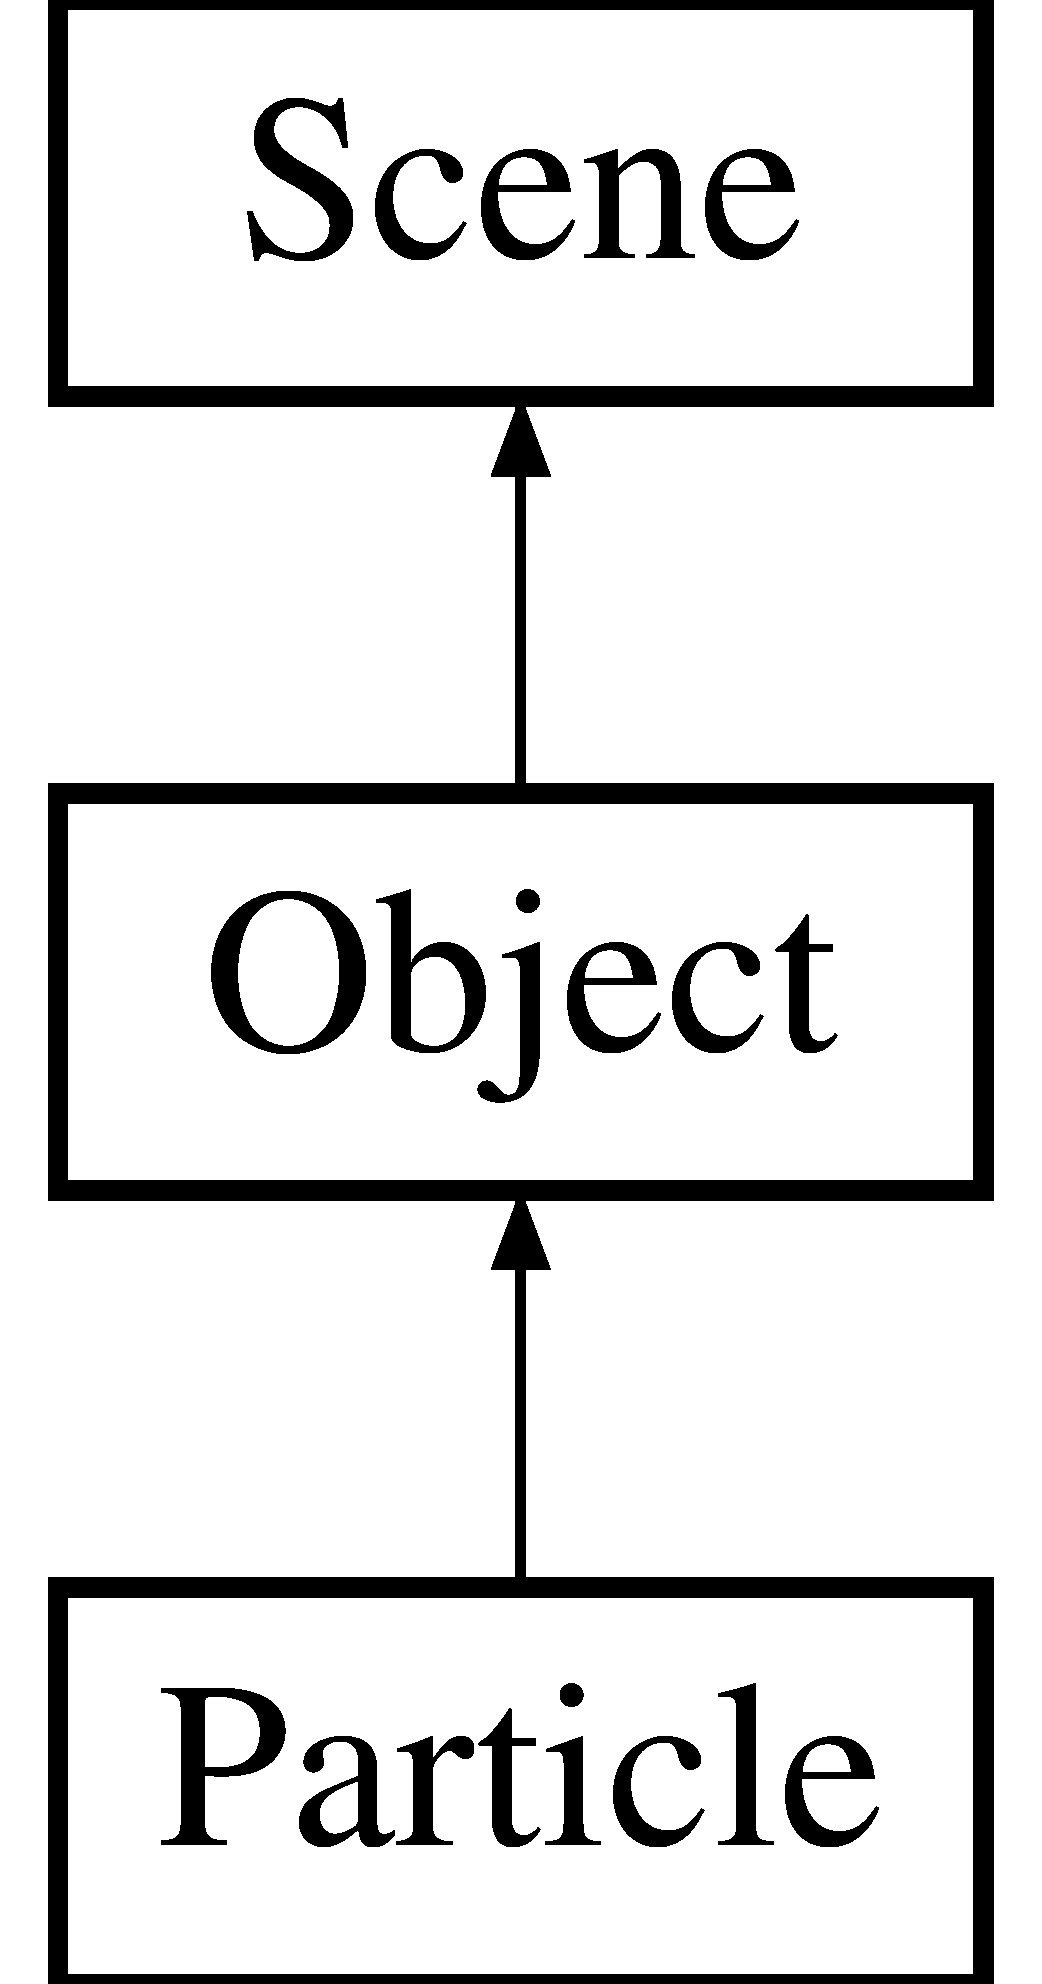
\includegraphics[height=3.000000cm]{class_particle}
\end{center}
\end{figure}
\subsection*{Public Types}
\begin{DoxyCompactItemize}
\item 
enum \hyperlink{class_object_a8c11d8700b0bb79a46c61f2de4f23fa3}{Uniforms} \{ \\*
\hyperlink{class_object_a8c11d8700b0bb79a46c61f2de4f23fa3a8a65225741e4db1df295c9cab71a98c0}{B\-E\-G\-I\-N}, 
\hyperlink{class_object_a8c11d8700b0bb79a46c61f2de4f23fa3a8fecaee23530c9befe7feb5166e81484}{I\-S\-\_\-\-T\-E\-X\-T\-U\-R\-E\-D} = B\-E\-G\-I\-N, 
\hyperlink{class_object_a8c11d8700b0bb79a46c61f2de4f23fa3a9aaf45d5144b52065016b5b39e909851}{O\-B\-J\-E\-C\-T\-\_\-\-C\-T\-M}, 
\hyperlink{class_object_a8c11d8700b0bb79a46c61f2de4f23fa3ac93e286d52dad730ccf3fdab9b102902}{M\-O\-R\-P\-H\-\_\-\-P\-C\-T}, 
\\*
\hyperlink{class_object_a8c11d8700b0bb79a46c61f2de4f23fa3ad78facbf844c1259f464a49061e1d7ed}{E\-N\-D}
 \}
\begin{DoxyCompactList}\small\item\em enum Uniforms describes the properties of the base object that need to be visible to the G\-P\-U. \end{DoxyCompactList}\item 
typedef const unsigned int \hyperlink{class_object_a79b74057dbc5182b85c9c3ba8480fcf2}{Uniform\-Enum}
\begin{DoxyCompactList}\small\item\em The \hyperlink{class_object}{Object} class takes advantage of child-\/extendible enumerations. \end{DoxyCompactList}\item 
typedef std\-::map\\*
$<$ \hyperlink{class_object_a79b74057dbc5182b85c9c3ba8480fcf2}{Object\-::\-Uniform\-Enum}, \\*
std\-::string $>$ \hyperlink{class_object_a6e19bd8516360bff956408cbae33b878}{Uniform\-Map}
\begin{DoxyCompactList}\small\item\em We store mappings of Uniform Enumerations, The desired function of the var, to strings, the names of the variables. \end{DoxyCompactList}\item 
typedef enum \hyperlink{class_object_a8c11d8700b0bb79a46c61f2de4f23fa3}{Object\-::\-Uniforms} \hyperlink{class_object_ae6a2969ddca87d2c54b7cb1c131a7d60}{Uniform}
\begin{DoxyCompactList}\small\item\em enum Uniforms describes the properties of the base object that need to be visible to the G\-P\-U. \end{DoxyCompactList}\end{DoxyCompactItemize}
\subsection*{Public Member Functions}
\begin{DoxyCompactItemize}
\item 
\hypertarget{class_particle_afcdc6f92de4e525a67617fe9fee6ae5d}{{\bfseries Particle} (\hyperlink{struct_angel_1_1vec4}{vec4} init\-Pos, \hyperlink{struct_angel_1_1vec3}{vec3} init\-Scale, \hyperlink{struct_angel_1_1vec3}{vec3} init\-Vel, float init\-Alpha, \hyperlink{struct_angel_1_1vec4}{vec4} init\-Color, float init\-Lifespan, float init\-Spin, string init\-Tex)}\label{class_particle_afcdc6f92de4e525a67617fe9fee6ae5d}

\item 
\hypertarget{class_particle_a686aad22bf7a80a089e117bbc7f4b738}{void {\bfseries update} ()}\label{class_particle_a686aad22bf7a80a089e117bbc7f4b738}

\item 
\hypertarget{class_particle_aabc36f29b35e0e1e5c6d6fb926bb7bbb}{void {\bfseries set\-Pos} (\hyperlink{struct_angel_1_1vec4}{vec4} new\-Pos)}\label{class_particle_aabc36f29b35e0e1e5c6d6fb926bb7bbb}

\item 
\hypertarget{class_particle_a1cdeee73a5eb04f48c0002f7136852ff}{void {\bfseries set\-Scale} (\hyperlink{struct_angel_1_1vec3}{vec3} new\-Scale)}\label{class_particle_a1cdeee73a5eb04f48c0002f7136852ff}

\item 
\hypertarget{class_particle_ac77b501936d44053585151c83b66ba22}{void {\bfseries set\-Vel} (\hyperlink{struct_angel_1_1vec3}{vec3} new\-Vel)}\label{class_particle_ac77b501936d44053585151c83b66ba22}

\item 
\hypertarget{class_particle_a3d339beee1c13eb3d1eed69d14715106}{void {\bfseries set\-Alpha} (float new\-Alpha)}\label{class_particle_a3d339beee1c13eb3d1eed69d14715106}

\item 
\hypertarget{class_particle_a8dbaf5f085a47c834c02f0531ccdbae1}{void {\bfseries set\-Color} (\hyperlink{struct_angel_1_1vec4}{vec4} new\-Color)}\label{class_particle_a8dbaf5f085a47c834c02f0531ccdbae1}

\item 
\hypertarget{class_particle_a2f59e88a58a6c6ea766ab4c94c75c2b3}{void {\bfseries set\-Lifespan} (float new\-Lifespan)}\label{class_particle_a2f59e88a58a6c6ea766ab4c94c75c2b3}

\item 
\hypertarget{class_particle_ac0cd12e63886b12d2b99549ecb552838}{void {\bfseries set\-Spin} (float new\-Spin)}\label{class_particle_ac0cd12e63886b12d2b99549ecb552838}

\item 
\hypertarget{class_particle_a5a387ad04e530af85dcd64763282d3a0}{void {\bfseries set\-Tex\-File} (string new\-Filename)}\label{class_particle_a5a387ad04e530af85dcd64763282d3a0}

\item 
\hypertarget{class_object_a53e2ee7f548550be014126bed139fe69}{void \hyperlink{class_object_a53e2ee7f548550be014126bed139fe69}{draw} (void)}\label{class_object_a53e2ee7f548550be014126bed139fe69}

\begin{DoxyCompactList}\small\item\em draw method\-: Render this object to the screen \-\_\-buffer. \end{DoxyCompactList}\item 
\hypertarget{class_object_a7edb92c30d86b6479b0ff2a5e9f06e13}{void \hyperlink{class_object_a7edb92c30d86b6479b0ff2a5e9f06e13}{buffer} (void)}\label{class_object_a7edb92c30d86b6479b0ff2a5e9f06e13}

\begin{DoxyCompactList}\small\item\em buffer all of our data\-: Vertices, Tex\-U\-Vs, Normals, Indices, Colors and Morph Buffers. \end{DoxyCompactList}\item 
\hypertarget{class_object_a293792abfe0671e00a0ec10e85ea9d9e}{void \hyperlink{class_object_a293792abfe0671e00a0ec10e85ea9d9e}{buffer\-Morph\-Only} (void)}\label{class_object_a293792abfe0671e00a0ec10e85ea9d9e}

\begin{DoxyCompactList}\small\item\em buffer only the Morph-\/related buffers. \end{DoxyCompactList}\item 
void \hyperlink{class_object_adafdf22583b051b4c61c8eb725fb07d5}{draw\-Mode} (G\-Lenum new\-\_\-mode)
\begin{DoxyCompactList}\small\item\em Select a new Open\-G\-L draw mode for this \hyperlink{class_object}{Object}. \end{DoxyCompactList}\item 
void \hyperlink{class_object_afebb27ddb10daed8e2c5085b76cbc500}{texture} (const char $\ast$$\ast$filename)
\begin{DoxyCompactList}\small\item\em F\-I\-X\-M\-E\-: This is a junk, nonflexible method. \end{DoxyCompactList}\item 
const std\-::string \& \hyperlink{class_object_aafd766fce2598f718cac97a3ac731706}{name} (void) const 
\begin{DoxyCompactList}\small\item\em Retrieve the \-\_\-name of this \hyperlink{class_object}{Object}. \end{DoxyCompactList}\item 
virtual void \hyperlink{class_object_a11d6063c580331d6af59c8d71b7f3e9f}{link} (\hyperlink{class_object_a79b74057dbc5182b85c9c3ba8480fcf2}{Uniform\-Enum} which, const std\-::string \&\hyperlink{class_object_aafd766fce2598f718cac97a3ac731706}{name})
\begin{DoxyCompactList}\small\item\em link a specified Uniform against the shader's variable \-\_\-name. \end{DoxyCompactList}\item 
virtual void \hyperlink{class_object_a34258ee199342d785c29d18c49d54e71}{send} (\hyperlink{class_object_a79b74057dbc5182b85c9c3ba8480fcf2}{Uniform\-Enum} which)
\begin{DoxyCompactList}\small\item\em Send a Uniform to the shader. \end{DoxyCompactList}\item 
virtual G\-Luint \hyperlink{class_object_a459489106838a1e3a8dbbd13045cd523}{shader} (void)
\begin{DoxyCompactList}\small\item\em Returns the \hyperlink{class_object}{Object}'s current shader. \end{DoxyCompactList}\item 
virtual void \hyperlink{class_object_aeaf11bb87bd59381c9e066f0b4f40d8e}{shader} (G\-Luint new\-Shader)
\begin{DoxyCompactList}\small\item\em Sets the shader to be used by this object. \end{DoxyCompactList}\item 
void \hyperlink{class_object_a0d604a816115c474b9593aeaebda9f8b}{animation} (void($\ast$anim\-\_\-func)(\hyperlink{class_trans_cache}{Trans\-Cache} \&arg))
\begin{DoxyCompactList}\small\item\em Apply an animation callback function to this \hyperlink{class_object}{Object}. \end{DoxyCompactList}\item 
void \hyperlink{class_object_a70a0f93ad9805057c5cc39853ce049c7}{propegate} (void)
\begin{DoxyCompactList}\small\item\em Scene-\/graph changes are not automatically applied to children. \end{DoxyCompactList}\item 
\hyperlink{struct_angel_1_1vec4}{vec4} \hyperlink{class_object_ac64609eb614aa5974b74000cec6fc95c}{position} () const 
\begin{DoxyCompactList}\small\item\em Obtain the vec4 representative of the \hyperlink{class_object}{Object}'s current position in space. \end{DoxyCompactList}\item 
\hyperlink{class_object}{Object} $\ast$ \hyperlink{class_object_a7694c9cfe445c3d5b993a38e3f8badd9}{morph\-Target} () const 
\begin{DoxyCompactList}\small\item\em Retrieve a pointer to this object's morph target. \end{DoxyCompactList}\item 
\hyperlink{class_object}{Object} $\ast$ \hyperlink{class_object_ab0ba603904f8f7de15dc0450e2d9b30e}{gen\-Morph\-Target} (G\-Luint \hyperlink{class_object_a459489106838a1e3a8dbbd13045cd523}{shader})
\begin{DoxyCompactList}\small\item\em Instantiate a new morphing target. \end{DoxyCompactList}\item 
float \hyperlink{class_object_accb051cdc79bc93e8c9c0edb79dd6b30}{morph\-Percentage} () const 
\begin{DoxyCompactList}\small\item\em Retrieve the morph Percentage of this object. \end{DoxyCompactList}\item 
void \hyperlink{class_object_a543d2329b25df9fb0a782f09d03e5cb1}{morph\-Percentage} (const float new\-Percentage)
\begin{DoxyCompactList}\small\item\em Set the morph percentage of this \hyperlink{class_object}{Object}. \end{DoxyCompactList}\item 
\hypertarget{class_object_a98d3f1b9ebb61c3b21e2a59ed267480a}{void \hyperlink{class_object_a98d3f1b9ebb61c3b21e2a59ed267480a}{destroy\-Morph\-Target} ()}\label{class_object_a98d3f1b9ebb61c3b21e2a59ed267480a}

\begin{DoxyCompactList}\small\item\em Obliterate the morph target for this object. \end{DoxyCompactList}\item 
int \hyperlink{class_object_a73f1a6210bacf504de9a808009479b81}{number\-Of\-Points} ()
\begin{DoxyCompactList}\small\item\em Retrieve the number of \-\_\-vertices this object has. \end{DoxyCompactList}\item 
\hypertarget{class_scene_aa5a48614e959c38c35d824fa9d6a4b8b}{\hyperlink{class_object}{Object} $\ast$ {\bfseries add\-Object} (const std\-::string \&obj\-Name, G\-Luint Object\-\_\-\-Shader=0)}\label{class_scene_aa5a48614e959c38c35d824fa9d6a4b8b}

\item 
\hypertarget{class_scene_a2a6845dacbb468c5c097c7a6ab5a0fe0}{void {\bfseries del\-Object} (const std\-::string \&obj\-Name)}\label{class_scene_a2a6845dacbb468c5c097c7a6ab5a0fe0}

\item 
\hypertarget{class_scene_a2e6b319b60e27e66ad43bb942a6c4424}{void {\bfseries del\-Object} (void)}\label{class_scene_a2e6b319b60e27e66ad43bb942a6c4424}

\item 
\hypertarget{class_scene_ad6c9d1d1d0c786d39bf97dc60410e28b}{void {\bfseries pop\-Object} (void)}\label{class_scene_ad6c9d1d1d0c786d39bf97dc60410e28b}

\item 
\hypertarget{class_scene_a8c57e1cebc39586c7928225d1e25de39}{void \hyperlink{class_scene_a8c57e1cebc39586c7928225d1e25de39}{destroy\-Object} (void)}\label{class_scene_a8c57e1cebc39586c7928225d1e25de39}

\begin{DoxyCompactList}\small\item\em Completely remove this object and all his children. \end{DoxyCompactList}\item 
\hypertarget{class_scene_a70fcdad192a4c6ff508125de8af6cf4d}{\hyperlink{class_object}{Object} $\ast$ {\bfseries next} (void)}\label{class_scene_a70fcdad192a4c6ff508125de8af6cf4d}

\item 
\hypertarget{class_scene_ac852d5d763eb35b4908c9aa7ea54d1ae}{\hyperlink{class_object}{Object} $\ast$ {\bfseries prev} (void)}\label{class_scene_ac852d5d763eb35b4908c9aa7ea54d1ae}

\item 
\hypertarget{class_scene_ad0ea1a6bcf7815c63988bd937f06eb23}{\hyperlink{class_object}{Object} $\ast$ {\bfseries active} (void) const }\label{class_scene_ad0ea1a6bcf7815c63988bd937f06eb23}

\item 
\hypertarget{class_scene_ae9b69d8db8a46991017635f22e45baad}{\hyperlink{class_object}{Object} $\ast$ {\bfseries operator\mbox{[}$\,$\mbox{]}} (const std\-::string \&objname)}\label{class_scene_ae9b69d8db8a46991017635f22e45baad}

\end{DoxyCompactItemize}
\subsection*{Public Attributes}
\begin{DoxyCompactItemize}
\item 
std\-::vector$<$ \hyperlink{struct_angel_1_1vec4}{Angel\-::vec4} $>$ \hyperlink{class_object_a4ac354b3ec284f27358b1d4b8d95b9a9}{\-\_\-vertices}
\begin{DoxyCompactList}\small\item\em vertex buffer. \end{DoxyCompactList}\item 
std\-::vector$<$ \hyperlink{struct_angel_1_1vec3}{Angel\-::vec3} $>$ \hyperlink{class_object_a20bb786cb5915934853855aab9d1a1b3}{\-\_\-normals}
\begin{DoxyCompactList}\small\item\em Normals buffer. \end{DoxyCompactList}\item 
std\-::vector$<$ unsigned int $>$ \hyperlink{class_object_ab85adc7a2d3b891051c096593982653d}{\-\_\-indices}
\begin{DoxyCompactList}\small\item\em Draw Order Index buffer. \end{DoxyCompactList}\item 
std\-::vector$<$ \hyperlink{struct_angel_1_1vec4}{Angel\-::vec4} $>$ \hyperlink{class_object_a29a0e9959c490067db69378bf57a17ba}{\-\_\-colors}
\begin{DoxyCompactList}\small\item\em Colors buffer. \end{DoxyCompactList}\item 
std\-::vector$<$ \hyperlink{struct_angel_1_1vec2}{Angel\-::vec2} $>$ \hyperlink{class_object_aa9ddc3b95d74b76ab8a251fb376dfafb}{\-\_\-tex\-U\-Vs}
\begin{DoxyCompactList}\small\item\em Texture Coordinates buffer. \end{DoxyCompactList}\item 
\hypertarget{class_object_af17d57ea2dab64e21112e8949d50d85f}{\hyperlink{class_trans_cache}{Trans\-Cache} \hyperlink{class_object_af17d57ea2dab64e21112e8949d50d85f}{\-\_\-trans}}\label{class_object_af17d57ea2dab64e21112e8949d50d85f}

\begin{DoxyCompactList}\small\item\em The \-\_\-trans cache encompasses the current transformational state of this object. \end{DoxyCompactList}\end{DoxyCompactItemize}
\subsection*{Protected Member Functions}
\begin{DoxyCompactItemize}
\item 
void \hyperlink{class_scene_ad3897f8ac658af62c133783b2c4eaee4}{delete\-Object} (\hyperlink{class_object}{Object} $\ast$obj)
\begin{DoxyCompactList}\small\item\em delete\-Object is the actual implementation function that will remove an \hyperlink{class_object}{Object} from the \hyperlink{class_scene}{Scene} list and \hyperlink{class_scene}{Scene} map, then free the object. \end{DoxyCompactList}\item 
\hypertarget{class_scene_ab64354bd8059bab589ca2dbf9de9e66c}{void {\bfseries insert\-Object} (const std\-::string \hyperlink{class_object_aafd766fce2598f718cac97a3ac731706}{name}, \hyperlink{class_object}{Object} $\ast$obj)}\label{class_scene_ab64354bd8059bab589ca2dbf9de9e66c}

\end{DoxyCompactItemize}
\subsection*{Protected Attributes}
\begin{DoxyCompactItemize}
\item 
std\-::string \hyperlink{class_object_a3f617214b260ebbe394e7c7b08ab5e43}{\-\_\-name}
\begin{DoxyCompactList}\small\item\em \-\_\-name is used as an identifying handle for the object. \end{DoxyCompactList}\item 
G\-Luint \hyperlink{class_object_a564aa6b1df66a05ab6b6c2f071851c4e}{\-\_\-vao}
\begin{DoxyCompactList}\small\item\em Vertex Array \hyperlink{class_object}{Object} handle identifying our buffers/object. \end{DoxyCompactList}\item 
\hypertarget{class_object_adf8365e2c661ab4014c3dbf60e48572b}{G\-Luint \hyperlink{class_object_adf8365e2c661ab4014c3dbf60e48572b}{\-\_\-buffer} \mbox{[}\hyperlink{class_object_a74a39247838865244defd0ae9712df9ba1999a38dc687c7ae05c884078de39b51}{N\-U\-M\-\_\-\-B\-U\-F\-F\-E\-R\-S}\mbox{]}}\label{class_object_adf8365e2c661ab4014c3dbf60e48572b}

\begin{DoxyCompactList}\small\item\em Handles to our buffers (Vertices, Tex\-U\-Vs, etc.) \end{DoxyCompactList}\item 
G\-Lenum \hyperlink{class_object_ae8457eabfb89d55826142508013b56c0}{\-\_\-draw\-Mode}
\begin{DoxyCompactList}\small\item\em Drawing mode for this object. \end{DoxyCompactList}\item 
\hypertarget{class_object_abcb877094b696561a49bc931c5a12d9f}{bool \hyperlink{class_object_abcb877094b696561a49bc931c5a12d9f}{\-\_\-is\-Textured}}\label{class_object_abcb877094b696561a49bc931c5a12d9f}

\begin{DoxyCompactList}\small\item\em Is this object textured? \end{DoxyCompactList}\item 
float \hyperlink{class_object_a7fbbac9027e1a8266342bd5ce064120d}{\-\_\-morph\-Percentage}
\begin{DoxyCompactList}\small\item\em The percentage of the morph. \end{DoxyCompactList}\item 
\hypertarget{class_object_a5baa9891bd4981d62b4e86a1c2a8eea7}{\hyperlink{class_object}{Object} $\ast$ \hyperlink{class_object_a5baa9891bd4981d62b4e86a1c2a8eea7}{\-\_\-morph\-Target}}\label{class_object_a5baa9891bd4981d62b4e86a1c2a8eea7}

\begin{DoxyCompactList}\small\item\em A pointer to the object we wish to morph into. \end{DoxyCompactList}\item 
std\-::map$<$ \hyperlink{class_object_a79b74057dbc5182b85c9c3ba8480fcf2}{Object\-::\-Uniform\-Enum}, \\*
std\-::string $>$ \hyperlink{class_object_a6378d0b0eeec23045ae2a5245e42bf13}{\-\_\-uniform\-Map}
\begin{DoxyCompactList}\small\item\em A map between Uniform variable functions and the actual uniform variable names. \end{DoxyCompactList}\item 
std\-::vector$<$ G\-Lint $>$ \hyperlink{class_object_a983963f564898beca4bda99676245663}{\-\_\-handles}
\begin{DoxyCompactList}\small\item\em Handles to Uniforms on the shader. \end{DoxyCompactList}\item 
\hypertarget{class_scene_acdd0123ca6b2d64d8d447bb485b235fc}{std\-::list$<$ \hyperlink{class_object}{Object} $\ast$ $>$ {\bfseries \-\_\-list}}\label{class_scene_acdd0123ca6b2d64d8d447bb485b235fc}

\item 
\hypertarget{class_scene_a8bd5d86484a12255b26b92b6cbf8d29a}{std\-::map$<$ std\-::string, \hyperlink{class_object}{Object} $\ast$ $>$ {\bfseries \-\_\-map}}\label{class_scene_a8bd5d86484a12255b26b92b6cbf8d29a}

\item 
\hypertarget{class_scene_ae87ca5350fcc595f3f15a4fd3c39f3d9}{std\-::list$<$ \hyperlink{class_object}{Object} $\ast$ $>$\-::iterator {\bfseries \-\_\-current\-Obj}}\label{class_scene_ae87ca5350fcc595f3f15a4fd3c39f3d9}

\item 
\hypertarget{class_scene_a8f9bdd8ec5edb1f414fbd314a36e2724}{G\-Luint {\bfseries \-\_\-g\-Shader}}\label{class_scene_a8f9bdd8ec5edb1f414fbd314a36e2724}

\end{DoxyCompactItemize}
\subsection*{Private Attributes}
\begin{DoxyCompactItemize}
\item 
\hypertarget{class_particle_a3d51791a544fb2cbf2e93531b3626132}{\hyperlink{struct_angel_1_1vec4}{vec4} {\bfseries m\-Pos}}\label{class_particle_a3d51791a544fb2cbf2e93531b3626132}

\item 
\hypertarget{class_particle_ad18c1ecffb2e5d032732d4cd058bb986}{\hyperlink{struct_angel_1_1vec3}{vec3} {\bfseries m\-Scale}}\label{class_particle_ad18c1ecffb2e5d032732d4cd058bb986}

\item 
\hypertarget{class_particle_a4cd8cbbc5b05126133df8246611339f2}{\hyperlink{struct_angel_1_1vec3}{vec3} {\bfseries m\-Vel}}\label{class_particle_a4cd8cbbc5b05126133df8246611339f2}

\item 
\hypertarget{class_particle_a14af67b37c2acfcbaffcc766b660a5f6}{float {\bfseries alpha}}\label{class_particle_a14af67b37c2acfcbaffcc766b660a5f6}

\item 
\hypertarget{class_particle_a3ec1cf194290dd222d3894e30a111db0}{\hyperlink{struct_angel_1_1vec4}{vec4} {\bfseries blend\-Color}}\label{class_particle_a3ec1cf194290dd222d3894e30a111db0}

\item 
\hypertarget{class_particle_a08108b2a0a2c0ec96f235510cc9aa0a2}{float {\bfseries lifespan}}\label{class_particle_a08108b2a0a2c0ec96f235510cc9aa0a2}

\item 
\hypertarget{class_particle_a73e6af7e8d30f1cbf570cc93fbe6529e}{float {\bfseries spin}}\label{class_particle_a73e6af7e8d30f1cbf570cc93fbe6529e}

\item 
\hypertarget{class_particle_a639147e87ea9fd39b04ac3bafb6ff97b}{string {\bfseries tex\-Filename}}\label{class_particle_a639147e87ea9fd39b04ac3bafb6ff97b}

\end{DoxyCompactItemize}


\subsection{Detailed Description}
T\-O\-D\-O\-: You know you've been bad. 

\begin{DoxyAuthor}{Author}
Nick Ver Voort, \href{mailto:nicholas_vervoort@student.uml.edu}{\tt nicholas\-\_\-vervoort@student.\-uml.\-edu} 
\end{DoxyAuthor}
\begin{DoxySince}{Since}
23 Feb 2013 
\end{DoxySince}


Definition at line 30 of file Particle.\-hpp.



\subsection{Member Typedef Documentation}
\hypertarget{class_object_ae6a2969ddca87d2c54b7cb1c131a7d60}{\index{Particle@{Particle}!Uniform@{Uniform}}
\index{Uniform@{Uniform}!Particle@{Particle}}
\subsubsection[{Uniform}]{\setlength{\rightskip}{0pt plus 5cm}typedef enum {\bf Object\-::\-Uniforms}  {\bf Object\-::\-Uniform}\hspace{0.3cm}{\ttfamily [inherited]}}}\label{class_object_ae6a2969ddca87d2c54b7cb1c131a7d60}


enum Uniforms describes the properties of the base object that need to be visible to the G\-P\-U. 

B\-E\-G\-I\-N and E\-N\-D are special sentinel enumerations that must be first and last, respectively. \hypertarget{class_object_a79b74057dbc5182b85c9c3ba8480fcf2}{\index{Particle@{Particle}!Uniform\-Enum@{Uniform\-Enum}}
\index{Uniform\-Enum@{Uniform\-Enum}!Particle@{Particle}}
\subsubsection[{Uniform\-Enum}]{\setlength{\rightskip}{0pt plus 5cm}typedef const unsigned int {\bf Object\-::\-Uniform\-Enum}\hspace{0.3cm}{\ttfamily [inherited]}}}\label{class_object_a79b74057dbc5182b85c9c3ba8480fcf2}


The \hyperlink{class_object}{Object} class takes advantage of child-\/extendible enumerations. 

We create an alias here for sake of ease. 

Definition at line 62 of file Object.\-hpp.

\hypertarget{class_object_a6e19bd8516360bff956408cbae33b878}{\index{Particle@{Particle}!Uniform\-Map@{Uniform\-Map}}
\index{Uniform\-Map@{Uniform\-Map}!Particle@{Particle}}
\subsubsection[{Uniform\-Map}]{\setlength{\rightskip}{0pt plus 5cm}typedef std\-::map$<$ {\bf Object\-::\-Uniform\-Enum}, std\-::string $>$ {\bf Object\-::\-Uniform\-Map}\hspace{0.3cm}{\ttfamily [inherited]}}}\label{class_object_a6e19bd8516360bff956408cbae33b878}


We store mappings of Uniform Enumerations, The desired function of the var, to strings, the names of the variables. 

This is utilized if we ever switch this object's shader, so we can re-\/associate with the correct uniform locations. 

Definition at line 70 of file Object.\-hpp.



\subsection{Member Enumeration Documentation}
\hypertarget{class_object_a8c11d8700b0bb79a46c61f2de4f23fa3}{\index{Particle@{Particle}!Uniforms@{Uniforms}}
\index{Uniforms@{Uniforms}!Particle@{Particle}}
\subsubsection[{Uniforms}]{\setlength{\rightskip}{0pt plus 5cm}enum {\bf Object\-::\-Uniforms}\hspace{0.3cm}{\ttfamily [inherited]}}}\label{class_object_a8c11d8700b0bb79a46c61f2de4f23fa3}


enum Uniforms describes the properties of the base object that need to be visible to the G\-P\-U. 

B\-E\-G\-I\-N and E\-N\-D are special sentinel enumerations that must be first and last, respectively. \begin{Desc}
\item[Enumerator]\par
\begin{description}
\index{B\-E\-G\-I\-N@{B\-E\-G\-I\-N}!Particle@{Particle}}\index{Particle@{Particle}!B\-E\-G\-I\-N@{B\-E\-G\-I\-N}}\item[{\em 
\hypertarget{class_object_a8c11d8700b0bb79a46c61f2de4f23fa3a8a65225741e4db1df295c9cab71a98c0}{B\-E\-G\-I\-N}\label{class_object_a8c11d8700b0bb79a46c61f2de4f23fa3a8a65225741e4db1df295c9cab71a98c0}
}]B\-E\-G\-I\-N. \index{I\-S\-\_\-\-T\-E\-X\-T\-U\-R\-E\-D@{I\-S\-\_\-\-T\-E\-X\-T\-U\-R\-E\-D}!Particle@{Particle}}\index{Particle@{Particle}!I\-S\-\_\-\-T\-E\-X\-T\-U\-R\-E\-D@{I\-S\-\_\-\-T\-E\-X\-T\-U\-R\-E\-D}}\item[{\em 
\hypertarget{class_object_a8c11d8700b0bb79a46c61f2de4f23fa3a8fecaee23530c9befe7feb5166e81484}{I\-S\-\_\-\-T\-E\-X\-T\-U\-R\-E\-D}\label{class_object_a8c11d8700b0bb79a46c61f2de4f23fa3a8fecaee23530c9befe7feb5166e81484}
}]I\-S\-\_\-\-T\-E\-X\-T\-U\-R\-E\-D. \index{O\-B\-J\-E\-C\-T\-\_\-\-C\-T\-M@{O\-B\-J\-E\-C\-T\-\_\-\-C\-T\-M}!Particle@{Particle}}\index{Particle@{Particle}!O\-B\-J\-E\-C\-T\-\_\-\-C\-T\-M@{O\-B\-J\-E\-C\-T\-\_\-\-C\-T\-M}}\item[{\em 
\hypertarget{class_object_a8c11d8700b0bb79a46c61f2de4f23fa3a9aaf45d5144b52065016b5b39e909851}{O\-B\-J\-E\-C\-T\-\_\-\-C\-T\-M}\label{class_object_a8c11d8700b0bb79a46c61f2de4f23fa3a9aaf45d5144b52065016b5b39e909851}
}]O\-B\-J\-E\-C\-T\-\_\-\-C\-T\-M. \index{M\-O\-R\-P\-H\-\_\-\-P\-C\-T@{M\-O\-R\-P\-H\-\_\-\-P\-C\-T}!Particle@{Particle}}\index{Particle@{Particle}!M\-O\-R\-P\-H\-\_\-\-P\-C\-T@{M\-O\-R\-P\-H\-\_\-\-P\-C\-T}}\item[{\em 
\hypertarget{class_object_a8c11d8700b0bb79a46c61f2de4f23fa3ac93e286d52dad730ccf3fdab9b102902}{M\-O\-R\-P\-H\-\_\-\-P\-C\-T}\label{class_object_a8c11d8700b0bb79a46c61f2de4f23fa3ac93e286d52dad730ccf3fdab9b102902}
}]M\-O\-R\-P\-H\-\_\-\-P\-C\-T. \index{E\-N\-D@{E\-N\-D}!Particle@{Particle}}\index{Particle@{Particle}!E\-N\-D@{E\-N\-D}}\item[{\em 
\hypertarget{class_object_a8c11d8700b0bb79a46c61f2de4f23fa3ad78facbf844c1259f464a49061e1d7ed}{E\-N\-D}\label{class_object_a8c11d8700b0bb79a46c61f2de4f23fa3ad78facbf844c1259f464a49061e1d7ed}
}]E\-N\-D. \end{description}
\end{Desc}


Definition at line 79 of file Object.\-hpp.



\subsection{Member Function Documentation}
\hypertarget{class_object_a0d604a816115c474b9593aeaebda9f8b}{\index{Particle@{Particle}!animation@{animation}}
\index{animation@{animation}!Particle@{Particle}}
\subsubsection[{animation}]{\setlength{\rightskip}{0pt plus 5cm}void Object\-::animation (
\begin{DoxyParamCaption}
\item[{void($\ast$)({\bf Trans\-Cache} \&arg)}]{anim\-\_\-func}
\end{DoxyParamCaption}
)\hspace{0.3cm}{\ttfamily [inherited]}}}\label{class_object_a0d604a816115c474b9593aeaebda9f8b}


Apply an animation callback function to this \hyperlink{class_object}{Object}. 

Works once only\-: Does not save the function or automatically run on idle. 
\begin{DoxyParams}{Parameters}
{\em anim\-\_\-func} & The transformation/animation function to apply. \\
\hline
\end{DoxyParams}


Definition at line 485 of file Object.\-cpp.

\hypertarget{class_scene_ad3897f8ac658af62c133783b2c4eaee4}{\index{Particle@{Particle}!delete\-Object@{delete\-Object}}
\index{delete\-Object@{delete\-Object}!Particle@{Particle}}
\subsubsection[{delete\-Object}]{\setlength{\rightskip}{0pt plus 5cm}void Scene\-::delete\-Object (
\begin{DoxyParamCaption}
\item[{{\bf Object} $\ast$}]{obj}
\end{DoxyParamCaption}
)\hspace{0.3cm}{\ttfamily [protected]}, {\ttfamily [inherited]}}}\label{class_scene_ad3897f8ac658af62c133783b2c4eaee4}


delete\-Object is the actual implementation function that will remove an \hyperlink{class_object}{Object} from the \hyperlink{class_scene}{Scene} list and \hyperlink{class_scene}{Scene} map, then free the object. 


\begin{DoxyParams}{Parameters}
{\em obj} & The pointer to the object to free. \\
\hline
\end{DoxyParams}


Definition at line 76 of file Scene.\-cpp.

\hypertarget{class_object_adafdf22583b051b4c61c8eb725fb07d5}{\index{Particle@{Particle}!draw\-Mode@{draw\-Mode}}
\index{draw\-Mode@{draw\-Mode}!Particle@{Particle}}
\subsubsection[{draw\-Mode}]{\setlength{\rightskip}{0pt plus 5cm}void Object\-::draw\-Mode (
\begin{DoxyParamCaption}
\item[{G\-Lenum}]{new\-\_\-mode}
\end{DoxyParamCaption}
)\hspace{0.3cm}{\ttfamily [inherited]}}}\label{class_object_adafdf22583b051b4c61c8eb725fb07d5}


Select a new Open\-G\-L draw mode for this \hyperlink{class_object}{Object}. 

Can be G\-L\-\_\-\-L\-I\-N\-E\-S, G\-L\-\_\-\-L\-I\-N\-E\-\_\-\-L\-O\-O\-P, G\-L\-\_\-\-T\-R\-I\-A\-N\-G\-L\-E\-S, etc. \begin{DoxySeeAlso}{See Also}
\href{http://www.opengl.org/wiki/Primitive}{\tt http\-://www.\-opengl.\-org/wiki/\-Primitive} 
\end{DoxySeeAlso}

\begin{DoxyParams}{Parameters}
{\em new\-\_\-mode} & The primitive rendering mode to use. \\
\hline
\end{DoxyParams}


Definition at line 267 of file Object.\-cpp.

\hypertarget{class_object_ab0ba603904f8f7de15dc0450e2d9b30e}{\index{Particle@{Particle}!gen\-Morph\-Target@{gen\-Morph\-Target}}
\index{gen\-Morph\-Target@{gen\-Morph\-Target}!Particle@{Particle}}
\subsubsection[{gen\-Morph\-Target}]{\setlength{\rightskip}{0pt plus 5cm}{\bf Object} $\ast$ Object\-::gen\-Morph\-Target (
\begin{DoxyParamCaption}
\item[{G\-Luint}]{shader}
\end{DoxyParamCaption}
)\hspace{0.3cm}{\ttfamily [inherited]}}}\label{class_object_ab0ba603904f8f7de15dc0450e2d9b30e}


Instantiate a new morphing target. 


\begin{DoxyParams}{Parameters}
{\em shader} & The shader to use for the new morphing target. N\-O\-T U\-S\-E\-D for rendering the object, but Objects cannot be instantiated without a shader, so here it is.\\
\hline
\end{DoxyParams}
\begin{DoxyReturn}{Returns}
A pointer to the newly created target. 
\end{DoxyReturn}


Definition at line 545 of file Object.\-cpp.

\hypertarget{class_object_a11d6063c580331d6af59c8d71b7f3e9f}{\index{Particle@{Particle}!link@{link}}
\index{link@{link}!Particle@{Particle}}
\subsubsection[{link}]{\setlength{\rightskip}{0pt plus 5cm}void Object\-::link (
\begin{DoxyParamCaption}
\item[{{\bf Uniform\-Enum}}]{which, }
\item[{const std\-::string \&}]{name}
\end{DoxyParamCaption}
)\hspace{0.3cm}{\ttfamily [virtual]}, {\ttfamily [inherited]}}}\label{class_object_a11d6063c580331d6af59c8d71b7f3e9f}


link a specified Uniform against the shader's variable \-\_\-name. 


\begin{DoxyParams}{Parameters}
{\em which} & The Uniform to link. \\
\hline
{\em name} & The variable \-\_\-name on the shader. \\
\hline
\end{DoxyParams}


Definition at line 392 of file Object.\-cpp.

\hypertarget{class_object_accb051cdc79bc93e8c9c0edb79dd6b30}{\index{Particle@{Particle}!morph\-Percentage@{morph\-Percentage}}
\index{morph\-Percentage@{morph\-Percentage}!Particle@{Particle}}
\subsubsection[{morph\-Percentage}]{\setlength{\rightskip}{0pt plus 5cm}float Object\-::morph\-Percentage (
\begin{DoxyParamCaption}
\item[{void}]{}
\end{DoxyParamCaption}
) const\hspace{0.3cm}{\ttfamily [inherited]}}}\label{class_object_accb051cdc79bc93e8c9c0edb79dd6b30}


Retrieve the morph Percentage of this object. 

\begin{DoxyReturn}{Returns}
The morph percentage, as a float. 
\end{DoxyReturn}


Definition at line 557 of file Object.\-cpp.

\hypertarget{class_object_a543d2329b25df9fb0a782f09d03e5cb1}{\index{Particle@{Particle}!morph\-Percentage@{morph\-Percentage}}
\index{morph\-Percentage@{morph\-Percentage}!Particle@{Particle}}
\subsubsection[{morph\-Percentage}]{\setlength{\rightskip}{0pt plus 5cm}void Object\-::morph\-Percentage (
\begin{DoxyParamCaption}
\item[{const float}]{new\-Percentage}
\end{DoxyParamCaption}
)\hspace{0.3cm}{\ttfamily [inherited]}}}\label{class_object_a543d2329b25df9fb0a782f09d03e5cb1}


Set the morph percentage of this \hyperlink{class_object}{Object}. 


\begin{DoxyParams}{Parameters}
{\em new\-Percentage} & The new morphing percentage. \\
\hline
\end{DoxyParams}


Definition at line 566 of file Object.\-cpp.

\hypertarget{class_object_a7694c9cfe445c3d5b993a38e3f8badd9}{\index{Particle@{Particle}!morph\-Target@{morph\-Target}}
\index{morph\-Target@{morph\-Target}!Particle@{Particle}}
\subsubsection[{morph\-Target}]{\setlength{\rightskip}{0pt plus 5cm}{\bf Object} $\ast$ Object\-::morph\-Target (
\begin{DoxyParamCaption}
\item[{void}]{}
\end{DoxyParamCaption}
) const\hspace{0.3cm}{\ttfamily [inherited]}}}\label{class_object_a7694c9cfe445c3d5b993a38e3f8badd9}


Retrieve a pointer to this object's morph target. 

\begin{DoxyReturn}{Returns}
An \hyperlink{class_object}{Object} pointer to the morph target. 
\end{DoxyReturn}


Definition at line 531 of file Object.\-cpp.

\hypertarget{class_object_aafd766fce2598f718cac97a3ac731706}{\index{Particle@{Particle}!name@{name}}
\index{name@{name}!Particle@{Particle}}
\subsubsection[{name}]{\setlength{\rightskip}{0pt plus 5cm}const std\-::string \& Object\-::name (
\begin{DoxyParamCaption}
\item[{void}]{}
\end{DoxyParamCaption}
) const\hspace{0.3cm}{\ttfamily [inherited]}}}\label{class_object_aafd766fce2598f718cac97a3ac731706}


Retrieve the \-\_\-name of this \hyperlink{class_object}{Object}. 

\begin{DoxyReturn}{Returns}
The \-\_\-name of this \hyperlink{class_object}{Object}. 
\end{DoxyReturn}


Definition at line 380 of file Object.\-cpp.

\hypertarget{class_object_a73f1a6210bacf504de9a808009479b81}{\index{Particle@{Particle}!number\-Of\-Points@{number\-Of\-Points}}
\index{number\-Of\-Points@{number\-Of\-Points}!Particle@{Particle}}
\subsubsection[{number\-Of\-Points}]{\setlength{\rightskip}{0pt plus 5cm}int Object\-::number\-Of\-Points (
\begin{DoxyParamCaption}
\item[{void}]{}
\end{DoxyParamCaption}
)\hspace{0.3cm}{\ttfamily [inherited]}}}\label{class_object_a73f1a6210bacf504de9a808009479b81}


Retrieve the number of \-\_\-vertices this object has. 

\begin{DoxyReturn}{Returns}
An integer representing the number of vertices the object has. 
\end{DoxyReturn}


Definition at line 586 of file Object.\-cpp.

\hypertarget{class_object_ac64609eb614aa5974b74000cec6fc95c}{\index{Particle@{Particle}!position@{position}}
\index{position@{position}!Particle@{Particle}}
\subsubsection[{position}]{\setlength{\rightskip}{0pt plus 5cm}{\bf vec4} Object\-::position (
\begin{DoxyParamCaption}
\item[{void}]{}
\end{DoxyParamCaption}
) const\hspace{0.3cm}{\ttfamily [inherited]}}}\label{class_object_ac64609eb614aa5974b74000cec6fc95c}


Obtain the vec4 representative of the \hyperlink{class_object}{Object}'s current position in space. 

\begin{DoxyReturn}{Returns}
vec4 representing the \hyperlink{class_object}{Object}'s position in space. 
\end{DoxyReturn}


Definition at line 520 of file Object.\-cpp.

\hypertarget{class_object_a70a0f93ad9805057c5cc39853ce049c7}{\index{Particle@{Particle}!propegate@{propegate}}
\index{propegate@{propegate}!Particle@{Particle}}
\subsubsection[{propegate}]{\setlength{\rightskip}{0pt plus 5cm}void Object\-::propegate (
\begin{DoxyParamCaption}
\item[{void}]{}
\end{DoxyParamCaption}
)\hspace{0.3cm}{\ttfamily [inherited]}}}\label{class_object_a70a0f93ad9805057c5cc39853ce049c7}


Scene-\/graph changes are not automatically applied to children. 

For efficiency reasons, you need to call \hyperlink{class_object_a70a0f93ad9805057c5cc39853ce049c7}{propegate()} manually. 

Definition at line 494 of file Object.\-cpp.

\hypertarget{class_object_a34258ee199342d785c29d18c49d54e71}{\index{Particle@{Particle}!send@{send}}
\index{send@{send}!Particle@{Particle}}
\subsubsection[{send}]{\setlength{\rightskip}{0pt plus 5cm}void Object\-::send (
\begin{DoxyParamCaption}
\item[{{\bf Object\-::\-Uniform\-Enum}}]{which}
\end{DoxyParamCaption}
)\hspace{0.3cm}{\ttfamily [virtual]}, {\ttfamily [inherited]}}}\label{class_object_a34258ee199342d785c29d18c49d54e71}


Send a Uniform to the shader. 


\begin{DoxyParams}{Parameters}
{\em which} & The uniform to send. \\
\hline
\end{DoxyParams}


Reimplemented in \hyperlink{class_camera_a401decef27b59d6485b4ab9762f5b9e6}{Camera}.



Definition at line 419 of file Object.\-cpp.

\hypertarget{class_object_a459489106838a1e3a8dbbd13045cd523}{\index{Particle@{Particle}!shader@{shader}}
\index{shader@{shader}!Particle@{Particle}}
\subsubsection[{shader}]{\setlength{\rightskip}{0pt plus 5cm}G\-Luint Object\-::shader (
\begin{DoxyParamCaption}
\item[{void}]{}
\end{DoxyParamCaption}
)\hspace{0.3cm}{\ttfamily [virtual]}, {\ttfamily [inherited]}}}\label{class_object_a459489106838a1e3a8dbbd13045cd523}


Returns the \hyperlink{class_object}{Object}'s current shader. 

Defined because C++ will not let you overload an overrided function, without re-\/overloading it in the derived class.

\begin{DoxyReturn}{Returns}
a G\-Luint handle to the shader program used by this \hyperlink{class_object}{Object}. 
\end{DoxyReturn}


Definition at line 448 of file Object.\-cpp.

\hypertarget{class_object_aeaf11bb87bd59381c9e066f0b4f40d8e}{\index{Particle@{Particle}!shader@{shader}}
\index{shader@{shader}!Particle@{Particle}}
\subsubsection[{shader}]{\setlength{\rightskip}{0pt plus 5cm}void Object\-::shader (
\begin{DoxyParamCaption}
\item[{G\-Luint}]{new\-Shader}
\end{DoxyParamCaption}
)\hspace{0.3cm}{\ttfamily [virtual]}, {\ttfamily [inherited]}}}\label{class_object_aeaf11bb87bd59381c9e066f0b4f40d8e}


Sets the shader to be used by this object. 

Triggers a query of the shader program, for the locations of the Uniform locations that the object needs.


\begin{DoxyParams}{Parameters}
{\em new\-Shader} & a G\-Luint handle to the shader program to use.\\
\hline
\end{DoxyParams}
\begin{DoxyReturn}{Returns}
None. 
\end{DoxyReturn}


Reimplemented from \hyperlink{class_scene_a3ea7e92935755c776c235a9872f53394}{Scene}.



Definition at line 464 of file Object.\-cpp.

\hypertarget{class_object_afebb27ddb10daed8e2c5085b76cbc500}{\index{Particle@{Particle}!texture@{texture}}
\index{texture@{texture}!Particle@{Particle}}
\subsubsection[{texture}]{\setlength{\rightskip}{0pt plus 5cm}void Object\-::texture (
\begin{DoxyParamCaption}
\item[{const char $\ast$$\ast$}]{filename}
\end{DoxyParamCaption}
)\hspace{0.3cm}{\ttfamily [inherited]}}}\label{class_object_afebb27ddb10daed8e2c5085b76cbc500}


F\-I\-X\-M\-E\-: This is a junk, nonflexible method. 

It would be better if you didn't think of this as being here.


\begin{DoxyParams}{Parameters}
{\em filename} & an array of strings to load textures from. \\
\hline
\end{DoxyParams}


Definition at line 277 of file Object.\-cpp.



\subsection{Member Data Documentation}
\hypertarget{class_object_a29a0e9959c490067db69378bf57a17ba}{\index{Particle@{Particle}!\-\_\-colors@{\-\_\-colors}}
\index{\-\_\-colors@{\-\_\-colors}!Particle@{Particle}}
\subsubsection[{\-\_\-colors}]{\setlength{\rightskip}{0pt plus 5cm}std\-::vector$<$ {\bf Angel\-::vec4} $>$ Object\-::\-\_\-colors\hspace{0.3cm}{\ttfamily [inherited]}}}\label{class_object_a29a0e9959c490067db69378bf57a17ba}


Colors buffer. 



Definition at line 246 of file Object.\-hpp.

\hypertarget{class_object_ae8457eabfb89d55826142508013b56c0}{\index{Particle@{Particle}!\-\_\-draw\-Mode@{\-\_\-draw\-Mode}}
\index{\-\_\-draw\-Mode@{\-\_\-draw\-Mode}!Particle@{Particle}}
\subsubsection[{\-\_\-draw\-Mode}]{\setlength{\rightskip}{0pt plus 5cm}G\-Lenum Object\-::\-\_\-draw\-Mode\hspace{0.3cm}{\ttfamily [protected]}, {\ttfamily [inherited]}}}\label{class_object_ae8457eabfb89d55826142508013b56c0}


Drawing mode for this object. 

G\-L\-\_\-\-T\-R\-I\-A\-N\-G\-L\-E\-S, G\-L\-\_\-\-L\-I\-N\-E\-\_\-\-L\-O\-O\-P, etc. 

Definition at line 268 of file Object.\-hpp.

\hypertarget{class_object_a983963f564898beca4bda99676245663}{\index{Particle@{Particle}!\-\_\-handles@{\-\_\-handles}}
\index{\-\_\-handles@{\-\_\-handles}!Particle@{Particle}}
\subsubsection[{\-\_\-handles}]{\setlength{\rightskip}{0pt plus 5cm}std\-::vector$<$ G\-Lint $>$ Object\-::\-\_\-handles\hspace{0.3cm}{\ttfamily [protected]}, {\ttfamily [inherited]}}}\label{class_object_a983963f564898beca4bda99676245663}


Handles to Uniforms on the shader. 

Protected to allow derived classes to extend it as needed. 

Definition at line 297 of file Object.\-hpp.

\hypertarget{class_object_ab85adc7a2d3b891051c096593982653d}{\index{Particle@{Particle}!\-\_\-indices@{\-\_\-indices}}
\index{\-\_\-indices@{\-\_\-indices}!Particle@{Particle}}
\subsubsection[{\-\_\-indices}]{\setlength{\rightskip}{0pt plus 5cm}std\-::vector$<$ unsigned int $>$ Object\-::\-\_\-indices\hspace{0.3cm}{\ttfamily [inherited]}}}\label{class_object_ab85adc7a2d3b891051c096593982653d}


Draw Order Index buffer. 

If not used, engine assumes G\-L\-\_\-\-D\-R\-A\-W\-\_\-\-A\-R\-R\-A\-Y\-S. 

Definition at line 244 of file Object.\-hpp.

\hypertarget{class_object_a7fbbac9027e1a8266342bd5ce064120d}{\index{Particle@{Particle}!\-\_\-morph\-Percentage@{\-\_\-morph\-Percentage}}
\index{\-\_\-morph\-Percentage@{\-\_\-morph\-Percentage}!Particle@{Particle}}
\subsubsection[{\-\_\-morph\-Percentage}]{\setlength{\rightskip}{0pt plus 5cm}float Object\-::\-\_\-morph\-Percentage\hspace{0.3cm}{\ttfamily [protected]}, {\ttfamily [inherited]}}}\label{class_object_a7fbbac9027e1a8266342bd5ce064120d}


The percentage of the morph. 

0.\-0 means 100\% the original, current object. 100.\-0 means 100\% the new, targeted object. 

Definition at line 279 of file Object.\-hpp.

\hypertarget{class_object_a3f617214b260ebbe394e7c7b08ab5e43}{\index{Particle@{Particle}!\-\_\-name@{\-\_\-name}}
\index{\-\_\-name@{\-\_\-name}!Particle@{Particle}}
\subsubsection[{\-\_\-name}]{\setlength{\rightskip}{0pt plus 5cm}std\-::string Object\-::\-\_\-name\hspace{0.3cm}{\ttfamily [protected]}, {\ttfamily [inherited]}}}\label{class_object_a3f617214b260ebbe394e7c7b08ab5e43}


\-\_\-name is used as an identifying handle for the object. 



Definition at line 259 of file Object.\-hpp.

\hypertarget{class_object_a20bb786cb5915934853855aab9d1a1b3}{\index{Particle@{Particle}!\-\_\-normals@{\-\_\-normals}}
\index{\-\_\-normals@{\-\_\-normals}!Particle@{Particle}}
\subsubsection[{\-\_\-normals}]{\setlength{\rightskip}{0pt plus 5cm}std\-::vector$<$ {\bf Angel\-::vec3} $>$ Object\-::\-\_\-normals\hspace{0.3cm}{\ttfamily [inherited]}}}\label{class_object_a20bb786cb5915934853855aab9d1a1b3}


Normals buffer. 



Definition at line 242 of file Object.\-hpp.

\hypertarget{class_object_aa9ddc3b95d74b76ab8a251fb376dfafb}{\index{Particle@{Particle}!\-\_\-tex\-U\-Vs@{\-\_\-tex\-U\-Vs}}
\index{\-\_\-tex\-U\-Vs@{\-\_\-tex\-U\-Vs}!Particle@{Particle}}
\subsubsection[{\-\_\-tex\-U\-Vs}]{\setlength{\rightskip}{0pt plus 5cm}std\-::vector$<$ {\bf Angel\-::vec2} $>$ Object\-::\-\_\-tex\-U\-Vs\hspace{0.3cm}{\ttfamily [inherited]}}}\label{class_object_aa9ddc3b95d74b76ab8a251fb376dfafb}


Texture Coordinates buffer. 



Definition at line 248 of file Object.\-hpp.

\hypertarget{class_object_a6378d0b0eeec23045ae2a5245e42bf13}{\index{Particle@{Particle}!\-\_\-uniform\-Map@{\-\_\-uniform\-Map}}
\index{\-\_\-uniform\-Map@{\-\_\-uniform\-Map}!Particle@{Particle}}
\subsubsection[{\-\_\-uniform\-Map}]{\setlength{\rightskip}{0pt plus 5cm}std\-::map$<$ {\bf Object\-::\-Uniform\-Enum}, std\-::string $>$ Object\-::\-\_\-uniform\-Map\hspace{0.3cm}{\ttfamily [protected]}, {\ttfamily [inherited]}}}\label{class_object_a6378d0b0eeec23045ae2a5245e42bf13}


A map between Uniform variable functions and the actual uniform variable names. 

Used when linking against a shader. 

Definition at line 290 of file Object.\-hpp.

\hypertarget{class_object_a564aa6b1df66a05ab6b6c2f071851c4e}{\index{Particle@{Particle}!\-\_\-vao@{\-\_\-vao}}
\index{\-\_\-vao@{\-\_\-vao}!Particle@{Particle}}
\subsubsection[{\-\_\-vao}]{\setlength{\rightskip}{0pt plus 5cm}G\-Luint Object\-::\-\_\-vao\hspace{0.3cm}{\ttfamily [protected]}, {\ttfamily [inherited]}}}\label{class_object_a564aa6b1df66a05ab6b6c2f071851c4e}


Vertex Array \hyperlink{class_object}{Object} handle identifying our buffers/object. 



Definition at line 262 of file Object.\-hpp.

\hypertarget{class_object_a4ac354b3ec284f27358b1d4b8d95b9a9}{\index{Particle@{Particle}!\-\_\-vertices@{\-\_\-vertices}}
\index{\-\_\-vertices@{\-\_\-vertices}!Particle@{Particle}}
\subsubsection[{\-\_\-vertices}]{\setlength{\rightskip}{0pt plus 5cm}std\-::vector$<$ {\bf Angel\-::vec4} $>$ Object\-::\-\_\-vertices\hspace{0.3cm}{\ttfamily [inherited]}}}\label{class_object_a4ac354b3ec284f27358b1d4b8d95b9a9}


vertex buffer. 



Definition at line 240 of file Object.\-hpp.



The documentation for this class was generated from the following files\-:\begin{DoxyCompactItemize}
\item 
\hyperlink{_particle_8hpp}{Particle.\-hpp}\item 
\hyperlink{_particle_8cpp}{Particle.\-cpp}\end{DoxyCompactItemize}

\input{class_particle_system}
\hypertarget{class_rot_mat}{\section{Rot\-Mat Class Reference}
\label{class_rot_mat}\index{Rot\-Mat@{Rot\-Mat}}
}


Rotations.  




{\ttfamily \#include $<$Transformation.\-hpp$>$}

Inheritance diagram for Rot\-Mat\-:\begin{figure}[H]
\begin{center}
\leavevmode
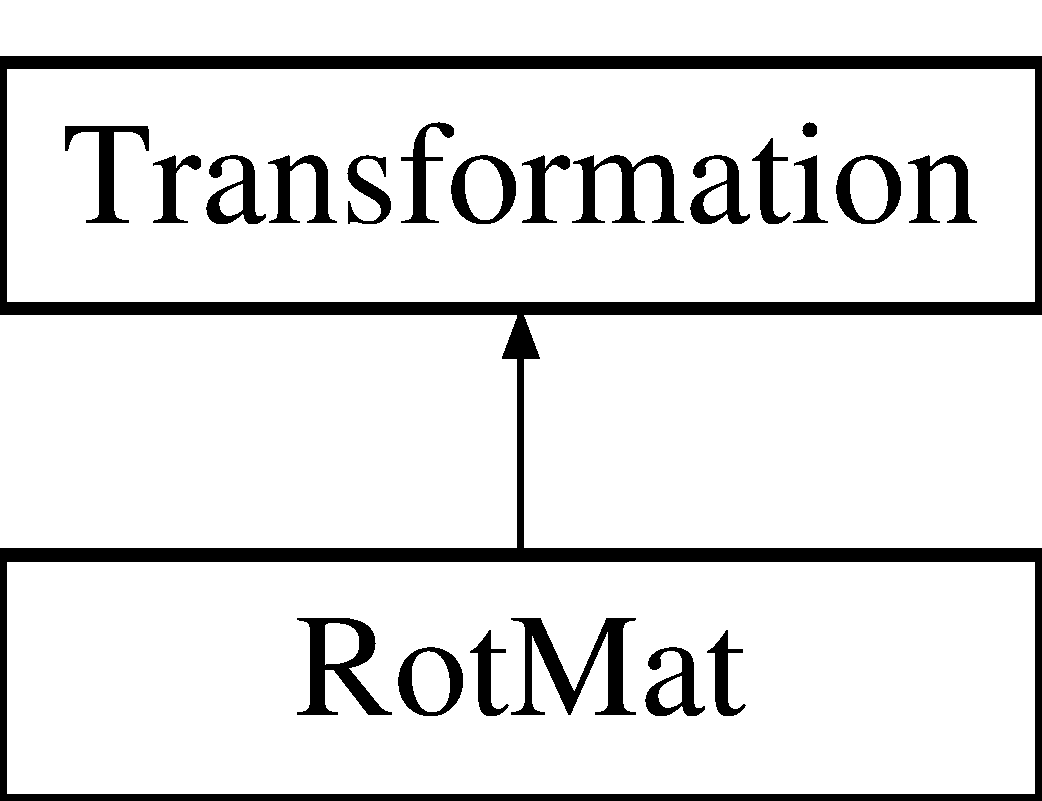
\includegraphics[height=2.000000cm]{class_rot_mat}
\end{center}
\end{figure}
\subsection*{Public Member Functions}
\begin{DoxyCompactItemize}
\item 
\hypertarget{class_rot_mat_a32b794d5158a61eccc2f9d7b06ab3fb5}{const \hyperlink{class_rot_mat}{Rot\-Mat} \& {\bfseries reset} (const \hyperlink{class_angel_1_1mat4}{Angel\-::mat4} \&New\-State)}\label{class_rot_mat_a32b794d5158a61eccc2f9d7b06ab3fb5}

\item 
\hypertarget{class_rot_mat_a15dbc3c6e4870662413e6998ad391191}{const \hyperlink{class_rot_mat}{Rot\-Mat} \& {\bfseries rotate\-X} (const G\-Lfloat theta, bool postmult=true)}\label{class_rot_mat_a15dbc3c6e4870662413e6998ad391191}

\item 
\hypertarget{class_rot_mat_ae1c4ec7d057458bf96ca94cd164617b8}{const \hyperlink{class_rot_mat}{Rot\-Mat} \& {\bfseries rotate\-Y} (const G\-Lfloat theta, bool postmult=true)}\label{class_rot_mat_ae1c4ec7d057458bf96ca94cd164617b8}

\item 
\hypertarget{class_rot_mat_a60364401770d127c040cc3ed1ad83c07}{const \hyperlink{class_rot_mat}{Rot\-Mat} \& {\bfseries rotate\-Z} (const G\-Lfloat theta, bool postmult=true)}\label{class_rot_mat_a60364401770d127c040cc3ed1ad83c07}

\item 
\hypertarget{class_rot_mat_ae37469da848ee4b633889f44babde9fe}{const \hyperlink{class_rot_mat}{Rot\-Mat} \& {\bfseries adjust} (const \hyperlink{class_angel_1_1mat4}{Angel\-::mat4} \&Adjustment, bool postmult=true)}\label{class_rot_mat_ae37469da848ee4b633889f44babde9fe}

\item 
\hypertarget{class_transformation_afcec300424207fc1d20864b73136937e}{const \hyperlink{class_angel_1_1mat4}{Angel\-::mat4} \& {\bfseries matrix} (void) const }\label{class_transformation_afcec300424207fc1d20864b73136937e}

\item 
\hypertarget{class_transformation_afdfbf48815a5b0d885f3b93f04cd2c66}{\hyperlink{class_angel_1_1mat4}{Angel\-::mat4} {\bfseries operator$\ast$} (const \hyperlink{class_angel_1_1mat4}{Angel\-::mat4} \&rhs) const }\label{class_transformation_afdfbf48815a5b0d885f3b93f04cd2c66}

\item 
\hypertarget{class_transformation_a85b923e0066365ef2e4aec3671396410}{\hyperlink{class_angel_1_1mat4}{Angel\-::mat4} {\bfseries operator$\ast$} (const \hyperlink{class_transformation}{Transformation} \&rhs) const }\label{class_transformation_a85b923e0066365ef2e4aec3671396410}

\end{DoxyCompactItemize}
\subsection*{Protected Attributes}
\begin{DoxyCompactItemize}
\item 
\hypertarget{class_transformation_a5f39fb578a1cdf78ca85efbd932d3834}{\hyperlink{class_angel_1_1mat4}{Angel\-::mat4} {\bfseries mat}}\label{class_transformation_a5f39fb578a1cdf78ca85efbd932d3834}

\end{DoxyCompactItemize}


\subsection{Detailed Description}
Rotations. 

Definition at line 40 of file Transformation.\-hpp.



The documentation for this class was generated from the following files\-:\begin{DoxyCompactItemize}
\item 
\hyperlink{_transformation_8hpp}{Transformation.\-hpp}\item 
\hyperlink{_transformation_8cpp}{Transformation.\-cpp}\end{DoxyCompactItemize}

\hypertarget{class_scale_mat}{\section{Scale\-Mat Class Reference}
\label{class_scale_mat}\index{Scale\-Mat@{Scale\-Mat}}
}
Inheritance diagram for Scale\-Mat\-:\begin{figure}[H]
\begin{center}
\leavevmode
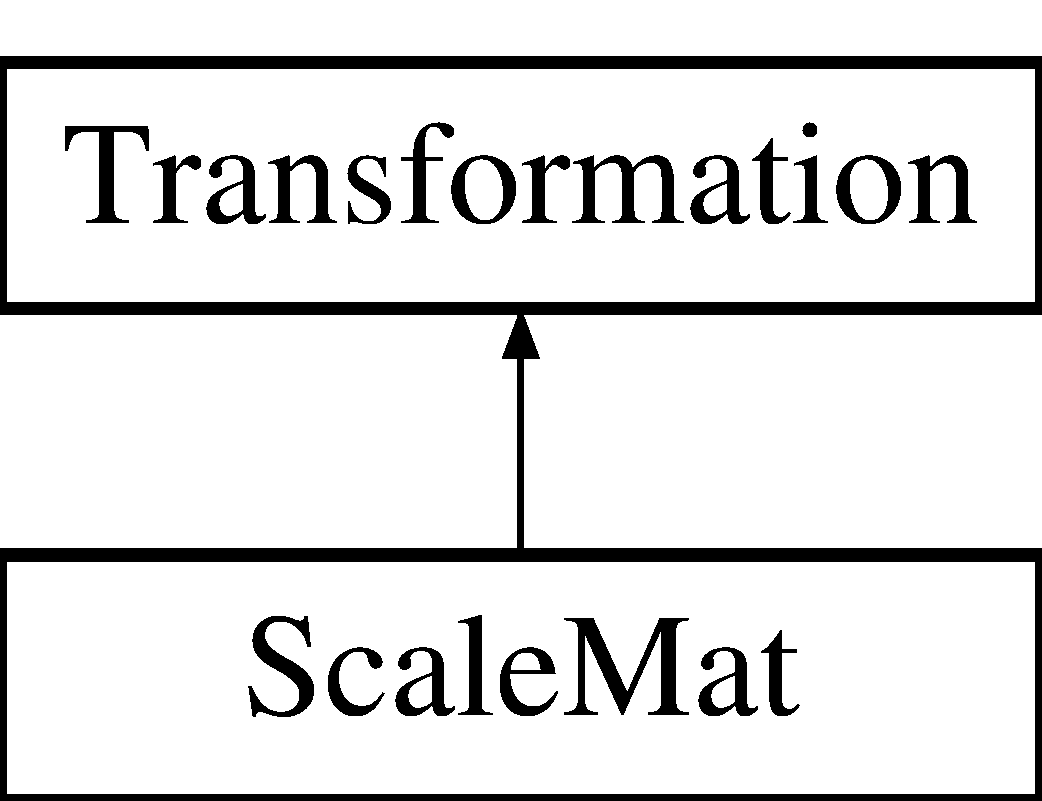
\includegraphics[height=2.000000cm]{class_scale_mat}
\end{center}
\end{figure}
\subsection*{Public Member Functions}
\begin{DoxyCompactItemize}
\item 
\hypertarget{class_scale_mat_ae8b855d2dc58511ab404d5c275936e7d}{const \hyperlink{class_scale_mat}{Scale\-Mat} \& {\bfseries set} (const float x, const float y, const float z)}\label{class_scale_mat_ae8b855d2dc58511ab404d5c275936e7d}

\item 
\hypertarget{class_scale_mat_a2c543c3aa6c795de16fba8cb40434a4f}{const \hyperlink{class_scale_mat}{Scale\-Mat} \& {\bfseries set} (const float pct)}\label{class_scale_mat_a2c543c3aa6c795de16fba8cb40434a4f}

\item 
\hypertarget{class_scale_mat_a6d6d05f3af9012223bb0b61530f18688}{const \hyperlink{class_scale_mat}{Scale\-Mat} \& {\bfseries adjust} (const float x, const float y, const float z)}\label{class_scale_mat_a6d6d05f3af9012223bb0b61530f18688}

\item 
\hypertarget{class_scale_mat_a5cb132a1dec58200eceaa33c4c619580}{const \hyperlink{class_scale_mat}{Scale\-Mat} \& {\bfseries adjust} (const float pct)}\label{class_scale_mat_a5cb132a1dec58200eceaa33c4c619580}

\item 
\hypertarget{class_transformation_afcec300424207fc1d20864b73136937e}{const \hyperlink{class_angel_1_1mat4}{Angel\-::mat4} \& {\bfseries matrix} (void) const }\label{class_transformation_afcec300424207fc1d20864b73136937e}

\item 
\hypertarget{class_transformation_afdfbf48815a5b0d885f3b93f04cd2c66}{\hyperlink{class_angel_1_1mat4}{Angel\-::mat4} {\bfseries operator$\ast$} (const \hyperlink{class_angel_1_1mat4}{Angel\-::mat4} \&rhs) const }\label{class_transformation_afdfbf48815a5b0d885f3b93f04cd2c66}

\item 
\hypertarget{class_transformation_a85b923e0066365ef2e4aec3671396410}{\hyperlink{class_angel_1_1mat4}{Angel\-::mat4} {\bfseries operator$\ast$} (const \hyperlink{class_transformation}{Transformation} \&rhs) const }\label{class_transformation_a85b923e0066365ef2e4aec3671396410}

\end{DoxyCompactItemize}
\subsection*{Protected Attributes}
\begin{DoxyCompactItemize}
\item 
\hypertarget{class_transformation_a5f39fb578a1cdf78ca85efbd932d3834}{\hyperlink{class_angel_1_1mat4}{Angel\-::mat4} {\bfseries mat}}\label{class_transformation_a5f39fb578a1cdf78ca85efbd932d3834}

\end{DoxyCompactItemize}


\subsection{Detailed Description}


Definition at line 70 of file Transformation.\-hpp.



The documentation for this class was generated from the following files\-:\begin{DoxyCompactItemize}
\item 
\hyperlink{_transformation_8hpp}{Transformation.\-hpp}\item 
\hyperlink{_transformation_8cpp}{Transformation.\-cpp}\end{DoxyCompactItemize}

\hypertarget{class_scene}{\section{Scene Class Reference}
\label{class_scene}\index{Scene@{Scene}}
}


The \hyperlink{class_scene}{Scene} object keeps track of a list of objects considered to be \char`\"{}children\char`\"{} of the \hyperlink{class_scene}{Scene}.  




{\ttfamily \#include $<$Scene.\-hpp$>$}

Inheritance diagram for Scene\-:\begin{figure}[H]
\begin{center}
\leavevmode
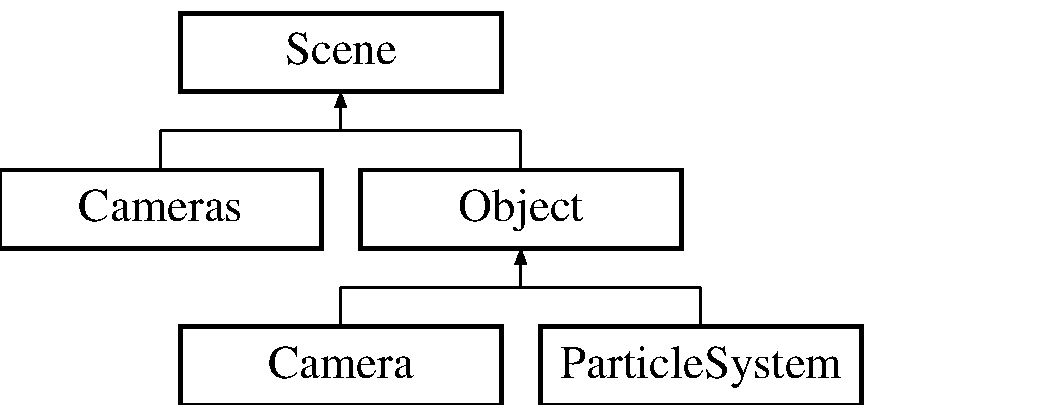
\includegraphics[height=3.000000cm]{class_scene}
\end{center}
\end{figure}
\subsection*{Public Member Functions}
\begin{DoxyCompactItemize}
\item 
\hypertarget{class_scene_ad10176d75a9cc0da56626f682d083507}{\hyperlink{class_scene_ad10176d75a9cc0da56626f682d083507}{Scene} ()}\label{class_scene_ad10176d75a9cc0da56626f682d083507}

\begin{DoxyCompactList}\small\item\em Nullary constructor. \end{DoxyCompactList}\item 
virtual \hyperlink{class_scene_a3b8cec2e32546713915f8c6303c951f1}{$\sim$\-Scene} ()
\begin{DoxyCompactList}\small\item\em Destructor! Will traverse its list and delete all objects! !! C\-A\-U\-T\-I\-O\-N !! If you have registered your own Objects manually, note that the scene will delete them for you! \end{DoxyCompactList}\item 
virtual void \hyperlink{class_scene_a3ea7e92935755c776c235a9872f53394}{shader} (G\-Luint g\-Shader)
\begin{DoxyCompactList}\small\item\em Sets the Default shader for the scene. \end{DoxyCompactList}\item 
G\-Luint \hyperlink{class_scene_a9d8a33f0f0a296aba0fb6717ab85cb18}{shader} (void)
\begin{DoxyCompactList}\small\item\em Retrieves the handle for the default shader for the scene. \end{DoxyCompactList}\item 
\hyperlink{class_object}{Object} $\ast$ \hyperlink{class_scene_aa5a48614e959c38c35d824fa9d6a4b8b}{add\-Object} (const std\-::string \&obj\-Name, G\-Luint Object\-\_\-\-Shader=0)
\begin{DoxyCompactList}\small\item\em add\-Object creates a new \hyperlink{class_object}{Object} with the given name and, optionally, a specified shader and adds it to the \hyperlink{class_scene}{Scene} graph. \end{DoxyCompactList}\item 
void \hyperlink{class_scene_a2a6845dacbb468c5c097c7a6ab5a0fe0}{del\-Object} (const std\-::string \&obj\-Name)
\begin{DoxyCompactList}\small\item\em del\-Object will remove from the \hyperlink{class_scene}{Scene} graph the object with the given name. \end{DoxyCompactList}\item 
\hypertarget{class_scene_a2e6b319b60e27e66ad43bb942a6c4424}{void \hyperlink{class_scene_a2e6b319b60e27e66ad43bb942a6c4424}{del\-Object} (void)}\label{class_scene_a2e6b319b60e27e66ad43bb942a6c4424}

\begin{DoxyCompactList}\small\item\em del\-Object with no parameters will delete the first \hyperlink{class_object}{Object} in the \hyperlink{class_scene}{Scene}. \end{DoxyCompactList}\item 
\hypertarget{class_scene_ad6c9d1d1d0c786d39bf97dc60410e28b}{void \hyperlink{class_scene_ad6c9d1d1d0c786d39bf97dc60410e28b}{pop\-Object} (void)}\label{class_scene_ad6c9d1d1d0c786d39bf97dc60410e28b}

\begin{DoxyCompactList}\small\item\em pop\-Object deletes the last \hyperlink{class_object}{Object} in the \hyperlink{class_scene}{Scene}. \end{DoxyCompactList}\item 
\hypertarget{class_scene_a70fcdad192a4c6ff508125de8af6cf4d}{\hyperlink{class_object}{Object} $\ast$ {\bfseries next} (void)}\label{class_scene_a70fcdad192a4c6ff508125de8af6cf4d}

\item 
\hypertarget{class_scene_ac852d5d763eb35b4908c9aa7ea54d1ae}{\hyperlink{class_object}{Object} $\ast$ {\bfseries prev} (void)}\label{class_scene_ac852d5d763eb35b4908c9aa7ea54d1ae}

\item 
\hypertarget{class_scene_ad0ea1a6bcf7815c63988bd937f06eb23}{\hyperlink{class_object}{Object} $\ast$ {\bfseries active} (void) const }\label{class_scene_ad0ea1a6bcf7815c63988bd937f06eb23}

\item 
\hypertarget{class_scene_a41fbbe388ea322df338648e66611ffcf}{void {\bfseries draw} (void)}\label{class_scene_a41fbbe388ea322df338648e66611ffcf}

\item 
\hypertarget{class_scene_ae9b69d8db8a46991017635f22e45baad}{\hyperlink{class_object}{Object} $\ast$ {\bfseries operator\mbox{[}$\,$\mbox{]}} (const std\-::string \&objname)}\label{class_scene_ae9b69d8db8a46991017635f22e45baad}

\item 
\hypertarget{class_scene_aa6e6354478dc7df82446b3abf9f91d96}{{\bfseries Scene} (const \hyperlink{class_scene}{Scene} \&copy)}\label{class_scene_aa6e6354478dc7df82446b3abf9f91d96}

\item 
\hypertarget{class_scene_a6336263b33b06ce4ace53599ffd8122c}{\hyperlink{class_scene}{Scene} \& {\bfseries operator=} (const \hyperlink{class_scene}{Scene} \&copy)}\label{class_scene_a6336263b33b06ce4ace53599ffd8122c}

\item 
void \hyperlink{class_scene_a8893899f0088a72642ae32a656252e7f}{insert\-Object} (\hyperlink{class_object}{Object} $\ast$obj)
\begin{DoxyCompactList}\small\item\em Register a created object with the scene graph. \end{DoxyCompactList}\end{DoxyCompactItemize}
\subsection*{Protected Member Functions}
\begin{DoxyCompactItemize}
\item 
void \hyperlink{class_scene_ad3897f8ac658af62c133783b2c4eaee4}{delete\-Object} (\hyperlink{class_object}{Object} $\ast$obj)
\begin{DoxyCompactList}\small\item\em Very seriously delete a child object and free his memory. \end{DoxyCompactList}\end{DoxyCompactItemize}
\subsection*{Protected Attributes}
\begin{DoxyCompactItemize}
\item 
\hypertarget{class_scene_acdd0123ca6b2d64d8d447bb485b235fc}{std\-::list$<$ \hyperlink{class_object}{Object} $\ast$ $>$ \hyperlink{class_scene_acdd0123ca6b2d64d8d447bb485b235fc}{\-\_\-list}}\label{class_scene_acdd0123ca6b2d64d8d447bb485b235fc}

\begin{DoxyCompactList}\small\item\em For the purposes of rapid propagation of scene-\/graph changes, \hyperlink{class_object}{Object} pointers are stored in a regular flat list. \end{DoxyCompactList}\item 
std\-::map$<$ std\-::string, \hyperlink{class_object}{Object} $\ast$ $>$ \hyperlink{class_scene_a8bd5d86484a12255b26b92b6cbf8d29a}{\-\_\-map}
\begin{DoxyCompactList}\small\item\em For the purposes of accessing named objects quickly, though, objects are also re-\/stored in an associative map. \end{DoxyCompactList}\item 
\hypertarget{class_scene_ae87ca5350fcc595f3f15a4fd3c39f3d9}{std\-::list$<$ \hyperlink{class_object}{Object} $\ast$ $>$\-::iterator \hyperlink{class_scene_ae87ca5350fcc595f3f15a4fd3c39f3d9}{\-\_\-current\-Obj}}\label{class_scene_ae87ca5350fcc595f3f15a4fd3c39f3d9}

\begin{DoxyCompactList}\small\item\em We keep an iterator on-\/hand that references what the scene considers to be it's active, current object. \end{DoxyCompactList}\item 
\hypertarget{class_scene_a8f9bdd8ec5edb1f414fbd314a36e2724}{G\-Luint \hyperlink{class_scene_a8f9bdd8ec5edb1f414fbd314a36e2724}{\-\_\-g\-Shader}}\label{class_scene_a8f9bdd8ec5edb1f414fbd314a36e2724}

\begin{DoxyCompactList}\small\item\em A handle to a shader program to be used as the default shader for new children objects added to the scene. \end{DoxyCompactList}\end{DoxyCompactItemize}


\subsection{Detailed Description}
The \hyperlink{class_scene}{Scene} object keeps track of a list of objects considered to be \char`\"{}children\char`\"{} of the \hyperlink{class_scene}{Scene}. 

The \hyperlink{class_scene}{Scene} itself has no physical representation or presence otherwise on the G\-P\-U, it is purely a logical C\-P\-U entity.

\begin{DoxyDate}{Date}
2013-\/03-\/16 
\end{DoxyDate}
\begin{DoxyAuthor}{Author}
John Huston 
\end{DoxyAuthor}


Definition at line 30 of file Scene.\-hpp.



\subsection{Constructor \& Destructor Documentation}
\hypertarget{class_scene_a3b8cec2e32546713915f8c6303c951f1}{\index{Scene@{Scene}!$\sim$\-Scene@{$\sim$\-Scene}}
\index{$\sim$\-Scene@{$\sim$\-Scene}!Scene@{Scene}}
\subsubsection[{$\sim$\-Scene}]{\setlength{\rightskip}{0pt plus 5cm}Scene\-::$\sim$\-Scene (
\begin{DoxyParamCaption}
{}
\end{DoxyParamCaption}
)\hspace{0.3cm}{\ttfamily [virtual]}}}\label{class_scene_a3b8cec2e32546713915f8c6303c951f1}


Destructor! Will traverse its list and delete all objects! !! C\-A\-U\-T\-I\-O\-N !! If you have registered your own Objects manually, note that the scene will delete them for you! 

You should, of course, never register objects from the stack. 

Definition at line 34 of file Scene.\-cpp.



\subsection{Member Function Documentation}
\hypertarget{class_scene_aa5a48614e959c38c35d824fa9d6a4b8b}{\index{Scene@{Scene}!add\-Object@{add\-Object}}
\index{add\-Object@{add\-Object}!Scene@{Scene}}
\subsubsection[{add\-Object}]{\setlength{\rightskip}{0pt plus 5cm}{\bf Object} $\ast$ Scene\-::add\-Object (
\begin{DoxyParamCaption}
\item[{const std\-::string \&}]{obj\-Name, }
\item[{G\-Luint}]{shader = {\ttfamily 0}}
\end{DoxyParamCaption}
)}}\label{class_scene_aa5a48614e959c38c35d824fa9d6a4b8b}


add\-Object creates a new \hyperlink{class_object}{Object} with the given name and, optionally, a specified shader and adds it to the \hyperlink{class_scene}{Scene} graph. 

If no shader is given, a default shader M\-U\-S\-T have been specified for the \hyperlink{class_scene}{Scene} prior to the call.


\begin{DoxyParams}{Parameters}
{\em obj\-Name} & The name of the new \hyperlink{class_object}{Object} to add. \\
\hline
{\em Object\-\_\-\-Shader} & The shader that should be used to render this object. \\
\hline
\end{DoxyParams}
\begin{DoxyReturn}{Returns}
A pointer to the new \hyperlink{class_object}{Object}. 
\end{DoxyReturn}


Definition at line 77 of file Scene.\-cpp.

\hypertarget{class_scene_ad3897f8ac658af62c133783b2c4eaee4}{\index{Scene@{Scene}!delete\-Object@{delete\-Object}}
\index{delete\-Object@{delete\-Object}!Scene@{Scene}}
\subsubsection[{delete\-Object}]{\setlength{\rightskip}{0pt plus 5cm}void Scene\-::delete\-Object (
\begin{DoxyParamCaption}
\item[{{\bf Object} $\ast$}]{obj}
\end{DoxyParamCaption}
)\hspace{0.3cm}{\ttfamily [protected]}}}\label{class_scene_ad3897f8ac658af62c133783b2c4eaee4}


Very seriously delete a child object and free his memory. 

delete\-Object is the actual implementation function that will remove an \hyperlink{class_object}{Object} from the \hyperlink{class_scene}{Scene} list and \hyperlink{class_scene}{Scene} map, then free the object.


\begin{DoxyParams}{Parameters}
{\em obj} & The object to delete.\\
\hline
{\em obj} & The pointer to the object to free. \\
\hline
\end{DoxyParams}


Definition at line 129 of file Scene.\-cpp.

\hypertarget{class_scene_a2a6845dacbb468c5c097c7a6ab5a0fe0}{\index{Scene@{Scene}!del\-Object@{del\-Object}}
\index{del\-Object@{del\-Object}!Scene@{Scene}}
\subsubsection[{del\-Object}]{\setlength{\rightskip}{0pt plus 5cm}void Scene\-::del\-Object (
\begin{DoxyParamCaption}
\item[{const std\-::string \&}]{obj\-Name}
\end{DoxyParamCaption}
)}}\label{class_scene_a2a6845dacbb468c5c097c7a6ab5a0fe0}


del\-Object will remove from the \hyperlink{class_scene}{Scene} graph the object with the given name. 


\begin{DoxyParams}{Parameters}
{\em obj\-Name} & Name of the \hyperlink{class_object}{Object} to delete. \\
\hline
\end{DoxyParams}


Definition at line 99 of file Scene.\-cpp.

\hypertarget{class_scene_a8893899f0088a72642ae32a656252e7f}{\index{Scene@{Scene}!insert\-Object@{insert\-Object}}
\index{insert\-Object@{insert\-Object}!Scene@{Scene}}
\subsubsection[{insert\-Object}]{\setlength{\rightskip}{0pt plus 5cm}void Scene\-::insert\-Object (
\begin{DoxyParamCaption}
\item[{{\bf Object} $\ast$}]{obj}
\end{DoxyParamCaption}
)}}\label{class_scene_a8893899f0088a72642ae32a656252e7f}


Register a created object with the scene graph. 


\begin{DoxyParams}{Parameters}
{\em name} & The name of the object (For the associative map), \\
\hline
{\em obj} & The \hyperlink{class_object}{Object} pointer to add to the scene. \\
\hline
\end{DoxyParams}


Definition at line 118 of file Scene.\-cpp.

\hypertarget{class_scene_a3ea7e92935755c776c235a9872f53394}{\index{Scene@{Scene}!shader@{shader}}
\index{shader@{shader}!Scene@{Scene}}
\subsubsection[{shader}]{\setlength{\rightskip}{0pt plus 5cm}void Scene\-::shader (
\begin{DoxyParamCaption}
\item[{G\-Luint}]{g\-Shader}
\end{DoxyParamCaption}
)\hspace{0.3cm}{\ttfamily [virtual]}}}\label{class_scene_a3ea7e92935755c776c235a9872f53394}


Sets the Default shader for the scene. 

In the context of inheritance by objects, This sets the shader to use to render the physical object.


\begin{DoxyParams}{Parameters}
{\em g\-Shader} & The G\-Luint handle to the shader to use.\\
\hline
\end{DoxyParams}
\begin{DoxyReturn}{Returns}
void. 
\end{DoxyReturn}


Reimplemented in \hyperlink{class_object_aeaf11bb87bd59381c9e066f0b4f40d8e}{Object}.



Definition at line 52 of file Scene.\-cpp.

\hypertarget{class_scene_a9d8a33f0f0a296aba0fb6717ab85cb18}{\index{Scene@{Scene}!shader@{shader}}
\index{shader@{shader}!Scene@{Scene}}
\subsubsection[{shader}]{\setlength{\rightskip}{0pt plus 5cm}G\-Luint Scene\-::shader (
\begin{DoxyParamCaption}
\item[{void}]{}
\end{DoxyParamCaption}
)}}\label{class_scene_a9d8a33f0f0a296aba0fb6717ab85cb18}


Retrieves the handle for the default shader for the scene. 

In the context of inheritance by objects, This retrieves the shader handle to use to draw the object.

\begin{DoxyReturn}{Returns}
A G\-Luint handle to the shader program. 
\end{DoxyReturn}


Reimplemented in \hyperlink{class_object_a459489106838a1e3a8dbbd13045cd523}{Object}.



Definition at line 63 of file Scene.\-cpp.



\subsection{Member Data Documentation}
\hypertarget{class_scene_a8bd5d86484a12255b26b92b6cbf8d29a}{\index{Scene@{Scene}!\-\_\-map@{\-\_\-map}}
\index{\-\_\-map@{\-\_\-map}!Scene@{Scene}}
\subsubsection[{\-\_\-map}]{\setlength{\rightskip}{0pt plus 5cm}std\-::map$<$ std\-::string, {\bf Object}$\ast$ $>$ Scene\-::\-\_\-map\hspace{0.3cm}{\ttfamily [protected]}}}\label{class_scene_a8bd5d86484a12255b26b92b6cbf8d29a}


For the purposes of accessing named objects quickly, though, objects are also re-\/stored in an associative map. 

It's a little superfluous, but here it is! 

Definition at line 127 of file Scene.\-hpp.



The documentation for this class was generated from the following files\-:\begin{DoxyCompactItemize}
\item 
\hyperlink{_scene_8hpp}{Scene.\-hpp}\item 
\hyperlink{_scene_8cpp}{Scene.\-cpp}\end{DoxyCompactItemize}

\hypertarget{class_screen}{\section{Screen Class Reference}
\label{class_screen}\index{Screen@{Screen}}
}
\subsection*{Public Member Functions}
\begin{DoxyCompactItemize}
\item 
\hypertarget{class_screen_ad97151af2e654778bad86043c32fe19f}{{\bfseries Screen} (int x=0, int y=0)}\label{class_screen_ad97151af2e654778bad86043c32fe19f}

\item 
\hypertarget{class_screen_a7b45282430392ffa8b5891936363f8f8}{{\bfseries Screen} (const \hyperlink{struct_angel_1_1vec2}{vec2} \&new\-Size)}\label{class_screen_a7b45282430392ffa8b5891936363f8f8}

\item 
\hypertarget{class_screen_a24e5be647130c965757db6cb9617fbe1}{void {\bfseries size} (int x, int y)}\label{class_screen_a24e5be647130c965757db6cb9617fbe1}

\item 
\hypertarget{class_screen_a2c027dc96b9133619687f21fd92d66ba}{void {\bfseries size} (const \hyperlink{struct_angel_1_1vec2}{vec2} \&new\-Size)}\label{class_screen_a2c027dc96b9133619687f21fd92d66ba}

\item 
\hypertarget{class_screen_a7c7219ac566e00e09bf3dd7df1a19ccd}{const \hyperlink{struct_angel_1_1vec2}{vec2} \& {\bfseries size} (void)}\label{class_screen_a7c7219ac566e00e09bf3dd7df1a19ccd}

\item 
\hypertarget{class_screen_aa411196a9c73a097e23e5e2cc6f4fb6d}{int {\bfseries width} (void)}\label{class_screen_aa411196a9c73a097e23e5e2cc6f4fb6d}

\item 
\hypertarget{class_screen_a492352f72fd2ee5f3cadcd553539bab1}{int {\bfseries height} (void)}\label{class_screen_a492352f72fd2ee5f3cadcd553539bab1}

\item 
\hypertarget{class_screen_ab1031780f278f25b9ad4efc0379e12fd}{const \hyperlink{struct_angel_1_1vec2}{vec2} \& {\bfseries center} (void)}\label{class_screen_ab1031780f278f25b9ad4efc0379e12fd}

\item 
\hypertarget{class_screen_a8ebfcb6f8f6a01c9397b0255e7e07b3e}{int {\bfseries midpoint\-X} (void)}\label{class_screen_a8ebfcb6f8f6a01c9397b0255e7e07b3e}

\item 
\hypertarget{class_screen_a4c579b4f3e27635f30b912d90a6b53d7}{int {\bfseries midpoint\-Y} (void)}\label{class_screen_a4c579b4f3e27635f30b912d90a6b53d7}

\end{DoxyCompactItemize}
\subsection*{Public Attributes}
\begin{DoxyCompactItemize}
\item 
\hypertarget{class_screen_a0098c32ec26cba2df8108d7b706986e5}{\hyperlink{class_cameras}{Cameras} {\bfseries \-\_\-cam\-List}}\label{class_screen_a0098c32ec26cba2df8108d7b706986e5}

\end{DoxyCompactItemize}
\subsection*{Private Attributes}
\begin{DoxyCompactItemize}
\item 
\hypertarget{class_screen_a02a1812a3807a9c4db6d4456861a7130}{\hyperlink{struct_angel_1_1vec2}{vec2} {\bfseries \-\_\-size}}\label{class_screen_a02a1812a3807a9c4db6d4456861a7130}

\item 
\hypertarget{class_screen_a1c82610b27dd93ae998b96d1fe11c792}{\hyperlink{struct_angel_1_1vec2}{vec2} {\bfseries \-\_\-center}}\label{class_screen_a1c82610b27dd93ae998b96d1fe11c792}

\end{DoxyCompactItemize}


\subsection{Detailed Description}


Definition at line 15 of file Screen.\-hpp.



The documentation for this class was generated from the following files\-:\begin{DoxyCompactItemize}
\item 
\hyperlink{_screen_8hpp}{Screen.\-hpp}\item 
\hyperlink{_screen_8cpp}{Screen.\-cpp}\end{DoxyCompactItemize}

\hypertarget{class_spelchk_camera}{\section{Spelchk\-Camera Class Reference}
\label{class_spelchk_camera}\index{Spelchk\-Camera@{Spelchk\-Camera}}
}
\subsection*{Public Member Functions}
\begin{DoxyCompactItemize}
\item 
\hypertarget{class_spelchk_camera_a1d894472ef9e588ddeb56434e549cd0a}{{\bfseries Spelchk\-Camera} (\hyperlink{struct_angel_1_1vec4}{vec4} initial\-Translation\-Vector)}\label{class_spelchk_camera_a1d894472ef9e588ddeb56434e549cd0a}

\item 
\hypertarget{class_spelchk_camera_a2a9aa83f6e5d3d2371dd00ae162aef30}{\hyperlink{class_angel_1_1mat4}{mat4} {\bfseries get\-Projection\-Matrix} ()}\label{class_spelchk_camera_a2a9aa83f6e5d3d2371dd00ae162aef30}

\item 
\hypertarget{class_spelchk_camera_af702dfbd3c3719e4b738440bb2269922}{\hyperlink{class_angel_1_1mat4}{mat4} {\bfseries get\-Model\-View\-Matrix} ()}\label{class_spelchk_camera_af702dfbd3c3719e4b738440bb2269922}

\item 
\hypertarget{class_spelchk_camera_a4ad8fbfe69914453580c02406bffc501}{\hyperlink{struct_angel_1_1vec4}{vec4} {\bfseries get\-Translation\-Vector} ()}\label{class_spelchk_camera_a4ad8fbfe69914453580c02406bffc501}

\item 
\hypertarget{class_spelchk_camera_a1396d6aa2a3e85d9ed8b90c17751da41}{void {\bfseries move\-Camera} (float x\-Depth, float y\-Depth, float z\-Depth)}\label{class_spelchk_camera_a1396d6aa2a3e85d9ed8b90c17751da41}

\item 
\hypertarget{class_spelchk_camera_aa012e2d10f196ae007a8f8b4ac8471c3}{void {\bfseries rotate\-Camera} (float x\-Angle, float y\-Angle, float z\-Angle)}\label{class_spelchk_camera_aa012e2d10f196ae007a8f8b4ac8471c3}

\item 
\hypertarget{class_spelchk_camera_a24f5fe7d296bcd7ec9d70b25b6a92fe5}{void {\bfseries set\-Screen\-Size} (int width, int height)}\label{class_spelchk_camera_a24f5fe7d296bcd7ec9d70b25b6a92fe5}

\item 
\hypertarget{class_spelchk_camera_a95b87c80007941d85d26c43d30fa7f87}{void {\bfseries set\-Projection} (int projection\-Type)}\label{class_spelchk_camera_a95b87c80007941d85d26c43d30fa7f87}

\item 
\hypertarget{class_spelchk_camera_a29d4ba987d9f3e1c47e1103fcea0ae2b}{void {\bfseries reset} ()}\label{class_spelchk_camera_a29d4ba987d9f3e1c47e1103fcea0ae2b}

\item 
\hypertarget{class_spelchk_camera_a20436fee96b0d6a1279d10b88e20f520}{void {\bfseries set\-Light\-Movement\-Ref} (G\-Luint ref)}\label{class_spelchk_camera_a20436fee96b0d6a1279d10b88e20f520}

\item 
\hypertarget{class_spelchk_camera_aed5d76d2de23473dec034161efe29275}{void {\bfseries set\-Light\-Movement\-Time} (float elapsed)}\label{class_spelchk_camera_aed5d76d2de23473dec034161efe29275}

\item 
\hypertarget{class_spelchk_camera_a90aa5e06ba61d44e63535acf2cc3e373}{void {\bfseries get\-Ready\-For\-Zero} (int usernum)}\label{class_spelchk_camera_a90aa5e06ba61d44e63535acf2cc3e373}

\item 
\hypertarget{class_spelchk_camera_afc39db6b4eab85070aa5d7494d0c5198}{void {\bfseries head\-Movement} (int usernum, double x, double y, double z)}\label{class_spelchk_camera_afc39db6b4eab85070aa5d7494d0c5198}

\end{DoxyCompactItemize}
\subsection*{Private Member Functions}
\begin{DoxyCompactItemize}
\item 
\hypertarget{class_spelchk_camera_a539230ff6d91932526666d4eee9d6c0d}{void {\bfseries calculate\-Translation\-Vector} ()}\label{class_spelchk_camera_a539230ff6d91932526666d4eee9d6c0d}

\end{DoxyCompactItemize}
\subsection*{Private Attributes}
\begin{DoxyCompactItemize}
\item 
\hypertarget{class_spelchk_camera_a1300ebc7e19c9784307668e5fbd54230}{int {\bfseries \-\_\-projection\-Type}}\label{class_spelchk_camera_a1300ebc7e19c9784307668e5fbd54230}

\item 
\hypertarget{class_spelchk_camera_a28e265ba33968587a514c40e1c188362}{G\-Lfloat {\bfseries \-\_\-fovy}}\label{class_spelchk_camera_a28e265ba33968587a514c40e1c188362}

\item 
\hypertarget{class_spelchk_camera_af45ecbaf2abdb45ba7a7b10988cb32bf}{G\-Lfloat {\bfseries \-\_\-aspect}}\label{class_spelchk_camera_af45ecbaf2abdb45ba7a7b10988cb32bf}

\item 
\hypertarget{class_spelchk_camera_a42693efc09de379317a24175a8820a4b}{G\-Lfloat {\bfseries \-\_\-left}}\label{class_spelchk_camera_a42693efc09de379317a24175a8820a4b}

\item 
\hypertarget{class_spelchk_camera_a4b673ae943e77ac4e84ef3655dffb9dc}{G\-Lfloat {\bfseries \-\_\-right}}\label{class_spelchk_camera_a4b673ae943e77ac4e84ef3655dffb9dc}

\item 
\hypertarget{class_spelchk_camera_a4b6008e072c2c969bdad94340c9e883f}{G\-Lfloat {\bfseries \-\_\-bottom}}\label{class_spelchk_camera_a4b6008e072c2c969bdad94340c9e883f}

\item 
\hypertarget{class_spelchk_camera_a4e57c23cb7296bf3b377b2695684f2f0}{G\-Lfloat {\bfseries \-\_\-top}}\label{class_spelchk_camera_a4e57c23cb7296bf3b377b2695684f2f0}

\item 
\hypertarget{class_spelchk_camera_a583fa3f337f6b4f6662c79580a7ac0b9}{G\-Lfloat {\bfseries \-\_\-z\-Near}}\label{class_spelchk_camera_a583fa3f337f6b4f6662c79580a7ac0b9}

\item 
\hypertarget{class_spelchk_camera_aa634e60867955c15ff1f3930fd65e141}{G\-Lfloat {\bfseries \-\_\-z\-Far}}\label{class_spelchk_camera_aa634e60867955c15ff1f3930fd65e141}

\item 
\hypertarget{class_spelchk_camera_a842fe340902238c352e3ae353c69efe3}{G\-Luint {\bfseries \-\_\-time\-Ref}}\label{class_spelchk_camera_a842fe340902238c352e3ae353c69efe3}

\item 
\hypertarget{class_spelchk_camera_a5af9cf826b28b2089f455b2a9dd55273}{int {\bfseries \-\_\-screen\-Width}}\label{class_spelchk_camera_a5af9cf826b28b2089f455b2a9dd55273}

\item 
\hypertarget{class_spelchk_camera_a71989db7bbd6ee6e53c449edbd5b97c2}{int {\bfseries \-\_\-screen\-Height}}\label{class_spelchk_camera_a71989db7bbd6ee6e53c449edbd5b97c2}

\item 
\hypertarget{class_spelchk_camera_af358d23e248c4ea34eac1cb6d43650c4}{G\-Lfloat {\bfseries \-\_\-x\-Depth}}\label{class_spelchk_camera_af358d23e248c4ea34eac1cb6d43650c4}

\item 
\hypertarget{class_spelchk_camera_ac9e259988d55580ca85a8ce675eca238}{G\-Lfloat {\bfseries \-\_\-y\-Depth}}\label{class_spelchk_camera_ac9e259988d55580ca85a8ce675eca238}

\item 
\hypertarget{class_spelchk_camera_a226c2bd8248e2da25449bb7b259cbe53}{G\-Lfloat {\bfseries \-\_\-z\-Depth}}\label{class_spelchk_camera_a226c2bd8248e2da25449bb7b259cbe53}

\item 
\hypertarget{class_spelchk_camera_affdf1796d7b273b022aab5bcd057906d}{G\-Lfloat {\bfseries \-\_\-x\-Angle}}\label{class_spelchk_camera_affdf1796d7b273b022aab5bcd057906d}

\item 
\hypertarget{class_spelchk_camera_aa91c493a5fcebf41dd22a2ba19dccb67}{G\-Lfloat {\bfseries \-\_\-y\-Angle}}\label{class_spelchk_camera_aa91c493a5fcebf41dd22a2ba19dccb67}

\item 
\hypertarget{class_spelchk_camera_aee718e71cfc0e1223a651640a92d043d}{G\-Lfloat {\bfseries \-\_\-z\-Angle}}\label{class_spelchk_camera_aee718e71cfc0e1223a651640a92d043d}

\item 
\hypertarget{class_spelchk_camera_aed4968712cd26cbcf1b3a0aaefef0be9}{G\-Lfloat {\bfseries \-\_\-x\-Head}}\label{class_spelchk_camera_aed4968712cd26cbcf1b3a0aaefef0be9}

\item 
\hypertarget{class_spelchk_camera_a8821e575424b9bf9c7df5b88a00791a9}{G\-Lfloat {\bfseries \-\_\-y\-Head}}\label{class_spelchk_camera_a8821e575424b9bf9c7df5b88a00791a9}

\item 
\hypertarget{class_spelchk_camera_a5b4f9fd0ac88b154a8ac7c67937a027e}{G\-Lfloat {\bfseries \-\_\-z\-Head}}\label{class_spelchk_camera_a5b4f9fd0ac88b154a8ac7c67937a027e}

\item 
\hypertarget{class_spelchk_camera_a1aee726b5d02ce0dfd94ab332a5bf2ae}{float {\bfseries \-\_\-x\-Head\-Start}}\label{class_spelchk_camera_a1aee726b5d02ce0dfd94ab332a5bf2ae}

\item 
\hypertarget{class_spelchk_camera_a15769e148b33d8a1ec1f66cb31113b5d}{float {\bfseries \-\_\-y\-Head\-Start}}\label{class_spelchk_camera_a15769e148b33d8a1ec1f66cb31113b5d}

\item 
\hypertarget{class_spelchk_camera_a2de115edea646f121f23948bd11acfc7}{float {\bfseries \-\_\-z\-Head\-Start}}\label{class_spelchk_camera_a2de115edea646f121f23948bd11acfc7}

\item 
\hypertarget{class_spelchk_camera_a81a21a91a20e88cdf22acf708049b514}{G\-Lfloat {\bfseries \-\_\-x\-Head\-Angle}}\label{class_spelchk_camera_a81a21a91a20e88cdf22acf708049b514}

\item 
\hypertarget{class_spelchk_camera_aa1aac3ac2dc8d81aa9c36808811748d2}{G\-Lfloat {\bfseries \-\_\-y\-Head\-Angle}}\label{class_spelchk_camera_aa1aac3ac2dc8d81aa9c36808811748d2}

\item 
\hypertarget{class_spelchk_camera_a53127a6e46ffee300cba7240768ecc84}{G\-Lfloat {\bfseries \-\_\-z\-Head\-Angle}}\label{class_spelchk_camera_a53127a6e46ffee300cba7240768ecc84}

\item 
\hypertarget{class_spelchk_camera_ab55d117dbbe81571f7647c99a8254c96}{\hyperlink{struct_angel_1_1vec4}{vec4} {\bfseries \-\_\-initial\-Translation\-Vector}}\label{class_spelchk_camera_ab55d117dbbe81571f7647c99a8254c96}

\item 
\hypertarget{class_spelchk_camera_ae6c14466dbc61908c0362d5d23a2e4d7}{\hyperlink{struct_angel_1_1vec4}{vec4} {\bfseries \-\_\-translation\-Vector}}\label{class_spelchk_camera_ae6c14466dbc61908c0362d5d23a2e4d7}

\item 
\hypertarget{class_spelchk_camera_a22330eebe446d1b1f2df252299af1bec}{\hyperlink{struct_angel_1_1vec4}{vec4} {\bfseries \-\_\-old\-Translation\-Vector}}\label{class_spelchk_camera_a22330eebe446d1b1f2df252299af1bec}

\item 
\hypertarget{class_spelchk_camera_a97affea96b6d50eb2f918e7a657211fa}{\hyperlink{class_angel_1_1mat4}{mat4} {\bfseries \-\_\-model\-View\-Matrix}}\label{class_spelchk_camera_a97affea96b6d50eb2f918e7a657211fa}

\item 
\hypertarget{class_spelchk_camera_a4d0112ca90bced7facf868165b109f2c}{int {\bfseries \-\_\-inbound\-Head\-Data}}\label{class_spelchk_camera_a4d0112ca90bced7facf868165b109f2c}

\item 
\hypertarget{class_spelchk_camera_a92d895ed8ba20382bcf9000acb8f62c4}{\hyperlink{struct_angel_1_1vec4}{vec4} {\bfseries \-\_\-initial\-Head\-Position}}\label{class_spelchk_camera_a92d895ed8ba20382bcf9000acb8f62c4}

\end{DoxyCompactItemize}


\subsection{Detailed Description}


Definition at line 17 of file Spelchk\-Camera.\-hpp.



The documentation for this class was generated from the following files\-:\begin{DoxyCompactItemize}
\item 
\hyperlink{_spelchk_camera_8hpp}{Spelchk\-Camera.\-hpp}\item 
\hyperlink{_spelchk_camera_8cpp}{Spelchk\-Camera.\-cpp}\end{DoxyCompactItemize}

\input{class_texture}
\hypertarget{class_timer}{\section{Timer Class Reference}
\label{class_timer}\index{Timer@{Timer}}
}
\subsection*{Public Member Functions}
\begin{DoxyCompactItemize}
\item 
unsigned long \hyperlink{class_timer_a303b48cd096028dbcc3d73f735c49b66}{tick} ()
\begin{DoxyCompactList}\small\item\em tick is an alias for tock. \end{DoxyCompactList}\item 
unsigned long \hyperlink{class_timer_a334900b3056fd3351c299fef28c31d3d}{tock} ()
\begin{DoxyCompactList}\small\item\em tock returns the time elapsed since the last tock. \end{DoxyCompactList}\item 
unsigned long \hyperlink{class_timer_a855136dd9e8cc3c07278dac9c4613693}{delta} () const 
\begin{DoxyCompactList}\small\item\em delta returns the time elapsed between the last tick and the last tock. \end{DoxyCompactList}\item 
\hypertarget{class_timer_a86957c3647a68e4d1666b4dc8765a631}{float {\bfseries key\-Frame\-Rate} () const }\label{class_timer_a86957c3647a68e4d1666b4dc8765a631}

\item 
\hypertarget{class_timer_ab49d5d4d56cfff329d3f3f4c74663ae2}{float {\bfseries key\-Frame\-Rate} (float new\-Frame\-Rate)}\label{class_timer_ab49d5d4d56cfff329d3f3f4c74663ae2}

\item 
double \hyperlink{class_timer_a7b3934948b0d2bc11a5e198e619b2576}{scale} () const 
\begin{DoxyCompactList}\small\item\em scale returns the relative lateness or eagerness of the \hyperlink{class_timer}{Timer}, Relative to a benchmark or Key Frame Rate (The default is 60\-F\-P\-S, or 16667 msec.) \end{DoxyCompactList}\end{DoxyCompactItemize}
\subsection*{Private Attributes}
\begin{DoxyCompactItemize}
\item 
\hypertarget{class_timer_af337d44bb179d24e7a462d05b36319fa}{struct timeval {\bfseries \-\_\-t1}}\label{class_timer_af337d44bb179d24e7a462d05b36319fa}

\item 
\hypertarget{class_timer_a093c39d8ce491d887ea0ae2e8d451030}{struct timeval {\bfseries \-\_\-t2}}\label{class_timer_a093c39d8ce491d887ea0ae2e8d451030}

\item 
\hypertarget{class_timer_a2a80ef1463e87f63e6ccc45a3fbe5ac2}{unsigned long {\bfseries \-\_\-delta}}\label{class_timer_a2a80ef1463e87f63e6ccc45a3fbe5ac2}

\item 
\hypertarget{class_timer_a02c5ec526c6bad4f0f2352325b4ac4f3}{double {\bfseries \-\_\-scale}}\label{class_timer_a02c5ec526c6bad4f0f2352325b4ac4f3}

\item 
\hypertarget{class_timer_af6e96c06b73154cd3a72ff22fb801e9e}{float {\bfseries \-\_\-key\-Frame\-Rate}}\label{class_timer_af6e96c06b73154cd3a72ff22fb801e9e}

\end{DoxyCompactItemize}


\subsection{Detailed Description}


Definition at line 14 of file Timer.\-hpp.



\subsection{Member Function Documentation}
\hypertarget{class_timer_a855136dd9e8cc3c07278dac9c4613693}{\index{Timer@{Timer}!delta@{delta}}
\index{delta@{delta}!Timer@{Timer}}
\subsubsection[{delta}]{\setlength{\rightskip}{0pt plus 5cm}unsigned long Timer\-::delta (
\begin{DoxyParamCaption}
\item[{void}]{}
\end{DoxyParamCaption}
) const}}\label{class_timer_a855136dd9e8cc3c07278dac9c4613693}


delta returns the time elapsed between the last tick and the last tock. 

Does not start a new timer. \begin{DoxyReturn}{Returns}
Time elapsed in Microseconds, or Nanoseconds if \-\_\-\-R\-T was enabled. 
\end{DoxyReturn}


Definition at line 74 of file Timer.\-cpp.

\hypertarget{class_timer_a7b3934948b0d2bc11a5e198e619b2576}{\index{Timer@{Timer}!scale@{scale}}
\index{scale@{scale}!Timer@{Timer}}
\subsubsection[{scale}]{\setlength{\rightskip}{0pt plus 5cm}double Timer\-::scale (
\begin{DoxyParamCaption}
\item[{void}]{}
\end{DoxyParamCaption}
) const}}\label{class_timer_a7b3934948b0d2bc11a5e198e619b2576}


scale returns the relative lateness or eagerness of the \hyperlink{class_timer}{Timer}, Relative to a benchmark or Key Frame Rate (The default is 60\-F\-P\-S, or 16667 msec.) 

\begin{DoxyReturn}{Returns}
A non-\/zero float that ranges from (0,1) indicating that the program is rendering faster than 60\-F\-P\-S, or from the range \mbox{[}1,+inf) indicating that the program is rendering slower than 60\-F\-P\-S. 
\end{DoxyReturn}


Definition at line 87 of file Timer.\-cpp.

\hypertarget{class_timer_a303b48cd096028dbcc3d73f735c49b66}{\index{Timer@{Timer}!tick@{tick}}
\index{tick@{tick}!Timer@{Timer}}
\subsubsection[{tick}]{\setlength{\rightskip}{0pt plus 5cm}unsigned long Timer\-::tick (
\begin{DoxyParamCaption}
\item[{void}]{}
\end{DoxyParamCaption}
)}}\label{class_timer_a303b48cd096028dbcc3d73f735c49b66}


tick is an alias for tock. 

Ha, Ha, Ha. \begin{DoxyReturn}{Returns}
An unsigned long corresponding to how much time has passed since the last tick. Microseconds normally, Nanoseconds if \-\_\-\-R\-T was enabled. 
\end{DoxyReturn}


Definition at line 44 of file Timer.\-cpp.

\hypertarget{class_timer_a334900b3056fd3351c299fef28c31d3d}{\index{Timer@{Timer}!tock@{tock}}
\index{tock@{tock}!Timer@{Timer}}
\subsubsection[{tock}]{\setlength{\rightskip}{0pt plus 5cm}unsigned long Timer\-::tock (
\begin{DoxyParamCaption}
\item[{void}]{}
\end{DoxyParamCaption}
)}}\label{class_timer_a334900b3056fd3351c299fef28c31d3d}


tock returns the time elapsed since the last tock. 

\begin{DoxyReturn}{Returns}
An unsigned long corresponding to how much time has passed since the last tock. Microseconds normally, Nanoseconds if \-\_\-\-R\-T was enabled. 
\end{DoxyReturn}


Definition at line 54 of file Timer.\-cpp.



The documentation for this class was generated from the following files\-:\begin{DoxyCompactItemize}
\item 
\hyperlink{_timer_8hpp}{Timer.\-hpp}\item 
\hyperlink{_timer_8cpp}{Timer.\-cpp}\end{DoxyCompactItemize}

\hypertarget{class_trans_cache}{\section{Trans\-Cache Class Reference}
\label{class_trans_cache}\index{Trans\-Cache@{Trans\-Cache}}
}
\subsection*{Public Member Functions}
\begin{DoxyCompactItemize}
\item 
\hypertarget{class_trans_cache_afbb46369dfa2169eaa30fcbf0038f8b8}{void {\bfseries ptm} (const \hyperlink{class_angel_1_1mat4}{Angel\-::mat4} \&ptm\-\_\-in, bool postmult=true)}\label{class_trans_cache_afbb46369dfa2169eaa30fcbf0038f8b8}

\item 
\hypertarget{class_trans_cache_a983b90a0f35e2955beb9a619c0c85ec3}{const \hyperlink{class_angel_1_1mat4}{Angel\-::mat4} \& {\bfseries ptm} (void) const }\label{class_trans_cache_a983b90a0f35e2955beb9a619c0c85ec3}

\item 
\hypertarget{class_trans_cache_a6a1d0e8050840494441f4be6cfdb02eb}{const \hyperlink{class_angel_1_1mat4}{Angel\-::mat4} \& {\bfseries ctm} (void) const }\label{class_trans_cache_a6a1d0e8050840494441f4be6cfdb02eb}

\item 
\hypertarget{class_trans_cache_a1c24bb0902fa8b1bc9ac306d28a6e079}{const \hyperlink{class_angel_1_1mat4}{Angel\-::mat4} \& {\bfseries otm} (void) const }\label{class_trans_cache_a1c24bb0902fa8b1bc9ac306d28a6e079}

\item 
\hypertarget{class_trans_cache_af35282cc89f14b468bafd65715a60f31}{void {\bfseries calc\-C\-T\-M} (bool postmult=true)}\label{class_trans_cache_af35282cc89f14b468bafd65715a60f31}

\end{DoxyCompactItemize}
\subsection*{Public Attributes}
\begin{DoxyCompactItemize}
\item 
\hypertarget{class_trans_cache_a1550ed069b59ac202af41716783ea452}{\hyperlink{class_trans_mat}{Trans\-Mat} {\bfseries \-\_\-pre\-Offset}}\label{class_trans_cache_a1550ed069b59ac202af41716783ea452}

\item 
\hypertarget{class_trans_cache_a01839c88c48f8e426e0d75a915ba7396}{\hyperlink{class_rot_mat}{Rot\-Mat} {\bfseries \-\_\-pre\-Rotation}}\label{class_trans_cache_a01839c88c48f8e426e0d75a915ba7396}

\item 
\hypertarget{class_trans_cache_acb34dfafde8ec9e0a2f6a4ed497905d4}{\hyperlink{class_scale_mat}{Scale\-Mat} {\bfseries \-\_\-scale}}\label{class_trans_cache_acb34dfafde8ec9e0a2f6a4ed497905d4}

\item 
\hypertarget{class_trans_cache_a7776dac55cc14489c7ec84661131d8f0}{\hyperlink{class_rot_mat}{Rot\-Mat} {\bfseries \-\_\-rotation}}\label{class_trans_cache_a7776dac55cc14489c7ec84661131d8f0}

\item 
\hypertarget{class_trans_cache_a9a67a280d50b47a456d0a07154a56a8d}{\hyperlink{class_trans_mat}{Trans\-Mat} {\bfseries \-\_\-offset}}\label{class_trans_cache_a9a67a280d50b47a456d0a07154a56a8d}

\item 
\hypertarget{class_trans_cache_a40698e1a82ecc629e15ad7149ea6205d}{\hyperlink{class_rot_mat}{Rot\-Mat} {\bfseries \-\_\-orbit}}\label{class_trans_cache_a40698e1a82ecc629e15ad7149ea6205d}

\item 
\hypertarget{class_trans_cache_a28f0d12b519c38de7be4ec640af011e9}{\hyperlink{class_trans_mat}{Trans\-Mat} {\bfseries \-\_\-displacement}}\label{class_trans_cache_a28f0d12b519c38de7be4ec640af011e9}

\end{DoxyCompactItemize}
\subsection*{Private Attributes}
\begin{DoxyCompactItemize}
\item 
\hypertarget{class_trans_cache_a3f620418592ae6bedde06d55261bba36}{\hyperlink{class_angel_1_1mat4}{Angel\-::mat4} {\bfseries \-\_\-ptm}}\label{class_trans_cache_a3f620418592ae6bedde06d55261bba36}

\item 
\hypertarget{class_trans_cache_a5bb6920889e36c616bd1648192ff5136}{\hyperlink{class_angel_1_1mat4}{Angel\-::mat4} {\bfseries \-\_\-ctm}}\label{class_trans_cache_a5bb6920889e36c616bd1648192ff5136}

\item 
\hypertarget{class_trans_cache_a968b1ec19687e1839f471658c63563a9}{\hyperlink{class_angel_1_1mat4}{Angel\-::mat4} {\bfseries \-\_\-otm}}\label{class_trans_cache_a968b1ec19687e1839f471658c63563a9}

\end{DoxyCompactItemize}


\subsection{Detailed Description}


Definition at line 14 of file Trans\-Cache.\-hpp.



The documentation for this class was generated from the following files\-:\begin{DoxyCompactItemize}
\item 
\hyperlink{_trans_cache_8hpp}{Trans\-Cache.\-hpp}\item 
\hyperlink{_trans_cache_8cpp}{Trans\-Cache.\-cpp}\end{DoxyCompactItemize}

\hypertarget{class_transformation}{\section{Transformation Class Reference}
\label{class_transformation}\index{Transformation@{Transformation}}
}
Inheritance diagram for Transformation\-:\begin{figure}[H]
\begin{center}
\leavevmode
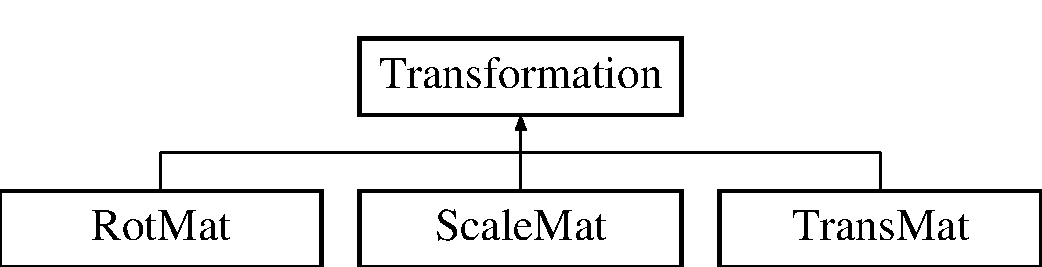
\includegraphics[height=2.000000cm]{class_transformation}
\end{center}
\end{figure}
\subsection*{Public Member Functions}
\begin{DoxyCompactItemize}
\item 
\hypertarget{class_transformation_afcec300424207fc1d20864b73136937e}{const \hyperlink{class_angel_1_1mat4}{Angel\-::mat4} \& {\bfseries matrix} (void) const }\label{class_transformation_afcec300424207fc1d20864b73136937e}

\item 
\hypertarget{class_transformation_afdfbf48815a5b0d885f3b93f04cd2c66}{\hyperlink{class_angel_1_1mat4}{Angel\-::mat4} {\bfseries operator$\ast$} (const \hyperlink{class_angel_1_1mat4}{Angel\-::mat4} \&rhs) const }\label{class_transformation_afdfbf48815a5b0d885f3b93f04cd2c66}

\item 
\hypertarget{class_transformation_a85b923e0066365ef2e4aec3671396410}{\hyperlink{class_angel_1_1mat4}{Angel\-::mat4} {\bfseries operator$\ast$} (const \hyperlink{class_transformation}{Transformation} \&rhs) const }\label{class_transformation_a85b923e0066365ef2e4aec3671396410}

\end{DoxyCompactItemize}
\subsection*{Protected Attributes}
\begin{DoxyCompactItemize}
\item 
\hypertarget{class_transformation_a5f39fb578a1cdf78ca85efbd932d3834}{\hyperlink{class_angel_1_1mat4}{Angel\-::mat4} {\bfseries mat}}\label{class_transformation_a5f39fb578a1cdf78ca85efbd932d3834}

\end{DoxyCompactItemize}


\subsection{Detailed Description}


Definition at line 16 of file Transformation.\-hpp.



The documentation for this class was generated from the following files\-:\begin{DoxyCompactItemize}
\item 
\hyperlink{_transformation_8hpp}{Transformation.\-hpp}\item 
\hyperlink{_transformation_8cpp}{Transformation.\-cpp}\end{DoxyCompactItemize}

\hypertarget{class_trans_mat}{\section{Trans\-Mat Class Reference}
\label{class_trans_mat}\index{Trans\-Mat@{Trans\-Mat}}
}


Translations.  




{\ttfamily \#include $<$Transformation.\-hpp$>$}

Inheritance diagram for Trans\-Mat\-:\begin{figure}[H]
\begin{center}
\leavevmode
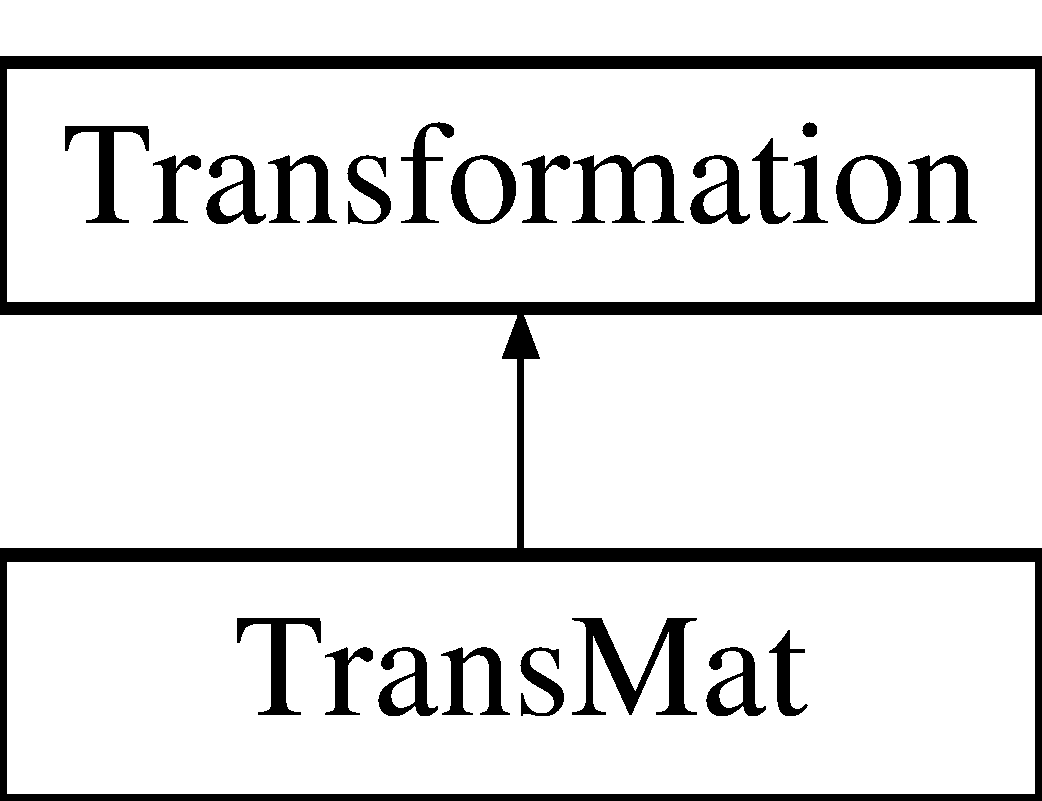
\includegraphics[height=2.000000cm]{class_trans_mat}
\end{center}
\end{figure}
\subsection*{Public Member Functions}
\begin{DoxyCompactItemize}
\item 
\hypertarget{class_trans_mat_afc0cc38bba734d8f668995cfbc263963}{const \hyperlink{class_trans_mat}{Trans\-Mat} \& {\bfseries set\-X} (const float x)}\label{class_trans_mat_afc0cc38bba734d8f668995cfbc263963}

\item 
\hypertarget{class_trans_mat_a97b2e285f76f35219389035b2121df69}{const \hyperlink{class_trans_mat}{Trans\-Mat} \& {\bfseries set\-Y} (const float y)}\label{class_trans_mat_a97b2e285f76f35219389035b2121df69}

\item 
\hypertarget{class_trans_mat_a957630c224fd750f0366a6422426ca43}{const \hyperlink{class_trans_mat}{Trans\-Mat} \& {\bfseries set\-Z} (const float z)}\label{class_trans_mat_a957630c224fd750f0366a6422426ca43}

\item 
\hypertarget{class_trans_mat_a4f4f05916524fb03c84a6a8e53769d52}{const \hyperlink{class_trans_mat}{Trans\-Mat} \& {\bfseries set} (const float x, const float y, const float z)}\label{class_trans_mat_a4f4f05916524fb03c84a6a8e53769d52}

\item 
\hypertarget{class_trans_mat_ac0b8a61381b2c7b21cc08d11e1959fd3}{const \hyperlink{class_trans_mat}{Trans\-Mat} \& {\bfseries set} (const \hyperlink{struct_angel_1_1vec3}{Angel\-::vec3} \&arg)}\label{class_trans_mat_ac0b8a61381b2c7b21cc08d11e1959fd3}

\item 
\hypertarget{class_trans_mat_abf67a3f4b41e34e423ebb921dace428f}{const \hyperlink{class_trans_mat}{Trans\-Mat} \& {\bfseries delta} (const float x, const float y, const float z)}\label{class_trans_mat_abf67a3f4b41e34e423ebb921dace428f}

\item 
\hypertarget{class_trans_mat_a4c93fe2c9ff1af5abf1ded66698cd297}{const \hyperlink{class_trans_mat}{Trans\-Mat} \& {\bfseries delta} (const \hyperlink{struct_angel_1_1vec3}{Angel\-::vec3} \&arg)}\label{class_trans_mat_a4c93fe2c9ff1af5abf1ded66698cd297}

\item 
\hypertarget{class_transformation_afcec300424207fc1d20864b73136937e}{const \hyperlink{class_angel_1_1mat4}{Angel\-::mat4} \& {\bfseries matrix} (void) const }\label{class_transformation_afcec300424207fc1d20864b73136937e}

\item 
\hypertarget{class_transformation_afdfbf48815a5b0d885f3b93f04cd2c66}{\hyperlink{class_angel_1_1mat4}{Angel\-::mat4} {\bfseries operator$\ast$} (const \hyperlink{class_angel_1_1mat4}{Angel\-::mat4} \&rhs) const }\label{class_transformation_afdfbf48815a5b0d885f3b93f04cd2c66}

\item 
\hypertarget{class_transformation_a85b923e0066365ef2e4aec3671396410}{\hyperlink{class_angel_1_1mat4}{Angel\-::mat4} {\bfseries operator$\ast$} (const \hyperlink{class_transformation}{Transformation} \&rhs) const }\label{class_transformation_a85b923e0066365ef2e4aec3671396410}

\end{DoxyCompactItemize}
\subsection*{Protected Attributes}
\begin{DoxyCompactItemize}
\item 
\hypertarget{class_transformation_a5f39fb578a1cdf78ca85efbd932d3834}{\hyperlink{class_angel_1_1mat4}{Angel\-::mat4} {\bfseries mat}}\label{class_transformation_a5f39fb578a1cdf78ca85efbd932d3834}

\end{DoxyCompactItemize}


\subsection{Detailed Description}
Translations. 

Definition at line 54 of file Transformation.\-hpp.



The documentation for this class was generated from the following files\-:\begin{DoxyCompactItemize}
\item 
\hyperlink{_transformation_8hpp}{Transformation.\-hpp}\item 
\hyperlink{_transformation_8cpp}{Transformation.\-cpp}\end{DoxyCompactItemize}

\hypertarget{struct_angel_1_1vec2}{\section{Angel\-:\-:vec2 Struct Reference}
\label{struct_angel_1_1vec2}\index{Angel\-::vec2@{Angel\-::vec2}}
}
\subsection*{Public Member Functions}
\begin{DoxyCompactItemize}
\item 
\hypertarget{struct_angel_1_1vec2_ab2463ddb6aaaa67251004b90f03530fa}{{\bfseries vec2} (G\-Lfloat s=G\-Lfloat(0.\-0))}\label{struct_angel_1_1vec2_ab2463ddb6aaaa67251004b90f03530fa}

\item 
\hypertarget{struct_angel_1_1vec2_a8e55cc0bb681ca7a747721cab122d830}{{\bfseries vec2} (G\-Lfloat x, G\-Lfloat y)}\label{struct_angel_1_1vec2_a8e55cc0bb681ca7a747721cab122d830}

\item 
\hypertarget{struct_angel_1_1vec2_aa2ec5b81c4b97019486b0595db6f35a1}{{\bfseries vec2} (const \hyperlink{struct_angel_1_1vec2}{vec2} \&v)}\label{struct_angel_1_1vec2_aa2ec5b81c4b97019486b0595db6f35a1}

\item 
\hypertarget{struct_angel_1_1vec2_a48235bf48a69717c273b72468d355244}{G\-Lfloat \& {\bfseries operator\mbox{[}$\,$\mbox{]}} (int i)}\label{struct_angel_1_1vec2_a48235bf48a69717c273b72468d355244}

\item 
\hypertarget{struct_angel_1_1vec2_a83725a082bca8ea73a2171bb4596c1bd}{const G\-Lfloat {\bfseries operator\mbox{[}$\,$\mbox{]}} (int i) const }\label{struct_angel_1_1vec2_a83725a082bca8ea73a2171bb4596c1bd}

\item 
\hypertarget{struct_angel_1_1vec2_a3b29693925c8026f75572dd13cefee5a}{\hyperlink{struct_angel_1_1vec2}{vec2} {\bfseries operator-\/} () const }\label{struct_angel_1_1vec2_a3b29693925c8026f75572dd13cefee5a}

\item 
\hypertarget{struct_angel_1_1vec2_a93606208e7b65d4bb8004f498b22934f}{\hyperlink{struct_angel_1_1vec2}{vec2} {\bfseries operator+} (const \hyperlink{struct_angel_1_1vec2}{vec2} \&v) const }\label{struct_angel_1_1vec2_a93606208e7b65d4bb8004f498b22934f}

\item 
\hypertarget{struct_angel_1_1vec2_a2d3d52e1b4693fdb860c2ef246e0d4d8}{\hyperlink{struct_angel_1_1vec2}{vec2} {\bfseries operator-\/} (const \hyperlink{struct_angel_1_1vec2}{vec2} \&v) const }\label{struct_angel_1_1vec2_a2d3d52e1b4693fdb860c2ef246e0d4d8}

\item 
\hypertarget{struct_angel_1_1vec2_ac5615b2494e3f8824f9fa127ba122b67}{\hyperlink{struct_angel_1_1vec2}{vec2} {\bfseries operator$\ast$} (const G\-Lfloat s) const }\label{struct_angel_1_1vec2_ac5615b2494e3f8824f9fa127ba122b67}

\item 
\hypertarget{struct_angel_1_1vec2_a3b4a9670b53342b870e3a14c8164c613}{\hyperlink{struct_angel_1_1vec2}{vec2} {\bfseries operator$\ast$} (const \hyperlink{struct_angel_1_1vec2}{vec2} \&v) const }\label{struct_angel_1_1vec2_a3b4a9670b53342b870e3a14c8164c613}

\item 
\hypertarget{struct_angel_1_1vec2_a522a6aaa64c361b86f6c2469cbd8ca92}{\hyperlink{struct_angel_1_1vec2}{vec2} {\bfseries operator/} (const G\-Lfloat s) const }\label{struct_angel_1_1vec2_a522a6aaa64c361b86f6c2469cbd8ca92}

\item 
\hypertarget{struct_angel_1_1vec2_aaa3b17cab0a568002fd965ef65e91653}{\hyperlink{struct_angel_1_1vec2}{vec2} \& {\bfseries operator+=} (const \hyperlink{struct_angel_1_1vec2}{vec2} \&v)}\label{struct_angel_1_1vec2_aaa3b17cab0a568002fd965ef65e91653}

\item 
\hypertarget{struct_angel_1_1vec2_ac48fa24fcdd901ab8748dda3361332f8}{\hyperlink{struct_angel_1_1vec2}{vec2} \& {\bfseries operator-\/=} (const \hyperlink{struct_angel_1_1vec2}{vec2} \&v)}\label{struct_angel_1_1vec2_ac48fa24fcdd901ab8748dda3361332f8}

\item 
\hypertarget{struct_angel_1_1vec2_a999ce51805c3c25a9a03039f05ce1492}{\hyperlink{struct_angel_1_1vec2}{vec2} \& {\bfseries operator$\ast$=} (const G\-Lfloat s)}\label{struct_angel_1_1vec2_a999ce51805c3c25a9a03039f05ce1492}

\item 
\hypertarget{struct_angel_1_1vec2_a8580b24c22b17ac08ab32841dcf03f45}{\hyperlink{struct_angel_1_1vec2}{vec2} \& {\bfseries operator$\ast$=} (const \hyperlink{struct_angel_1_1vec2}{vec2} \&v)}\label{struct_angel_1_1vec2_a8580b24c22b17ac08ab32841dcf03f45}

\item 
\hypertarget{struct_angel_1_1vec2_a6ea8be1d732aea09b0f3f16f61fa2ef7}{\hyperlink{struct_angel_1_1vec2}{vec2} \& {\bfseries operator/=} (const G\-Lfloat s)}\label{struct_angel_1_1vec2_a6ea8be1d732aea09b0f3f16f61fa2ef7}

\item 
\hypertarget{struct_angel_1_1vec2_a5c3d2082bcc18734fde3689dbc605104}{{\bfseries operator const G\-Lfloat $\ast$} () const }\label{struct_angel_1_1vec2_a5c3d2082bcc18734fde3689dbc605104}

\item 
\hypertarget{struct_angel_1_1vec2_a8989f46bc38bb87bc2f6ea81f66c8545}{{\bfseries operator G\-Lfloat $\ast$} ()}\label{struct_angel_1_1vec2_a8989f46bc38bb87bc2f6ea81f66c8545}

\end{DoxyCompactItemize}
\subsection*{Public Attributes}
\begin{DoxyCompactItemize}
\item 
\hypertarget{struct_angel_1_1vec2_ab99b91871c08bbf76bf4a5e554ccac8f}{G\-Lfloat {\bfseries x}}\label{struct_angel_1_1vec2_ab99b91871c08bbf76bf4a5e554ccac8f}

\item 
\hypertarget{struct_angel_1_1vec2_a9f0e4c33e7884eca47d771ccfd4ea0bd}{G\-Lfloat {\bfseries y}}\label{struct_angel_1_1vec2_a9f0e4c33e7884eca47d771ccfd4ea0bd}

\end{DoxyCompactItemize}
\subsection*{Friends}
\begin{DoxyCompactItemize}
\item 
\hypertarget{struct_angel_1_1vec2_a1f371c4b26f86deb4d296dfff8ff1fc1}{\hyperlink{struct_angel_1_1vec2}{vec2} {\bfseries operator$\ast$} (const G\-Lfloat s, const \hyperlink{struct_angel_1_1vec2}{vec2} \&v)}\label{struct_angel_1_1vec2_a1f371c4b26f86deb4d296dfff8ff1fc1}

\item 
\hypertarget{struct_angel_1_1vec2_a5533e582fe94db90861caa394494f2cf}{std\-::ostream \& {\bfseries operator$<$$<$} (std\-::ostream \&os, const \hyperlink{struct_angel_1_1vec2}{vec2} \&v)}\label{struct_angel_1_1vec2_a5533e582fe94db90861caa394494f2cf}

\item 
\hypertarget{struct_angel_1_1vec2_af8cf130207f2cf5866ac13049e956c75}{std\-::istream \& {\bfseries operator$>$$>$} (std\-::istream \&is, \hyperlink{struct_angel_1_1vec2}{vec2} \&v)}\label{struct_angel_1_1vec2_af8cf130207f2cf5866ac13049e956c75}

\end{DoxyCompactItemize}


\subsection{Detailed Description}


Definition at line 18 of file vec.\-hpp.



The documentation for this struct was generated from the following files\-:\begin{DoxyCompactItemize}
\item 
\hyperlink{vec_8hpp}{vec.\-hpp}\item 
\hyperlink{vec_8cpp}{vec.\-cpp}\end{DoxyCompactItemize}

\hypertarget{struct_angel_1_1vec3}{\section{Angel\-:\-:vec3 Struct Reference}
\label{struct_angel_1_1vec3}\index{Angel\-::vec3@{Angel\-::vec3}}
}
\subsection*{Public Member Functions}
\begin{DoxyCompactItemize}
\item 
\hypertarget{struct_angel_1_1vec3_a420358f913d30a659761e3a86026cd59}{{\bfseries vec3} (G\-Lfloat s=G\-Lfloat(0.\-0))}\label{struct_angel_1_1vec3_a420358f913d30a659761e3a86026cd59}

\item 
\hypertarget{struct_angel_1_1vec3_a9970b9133cd349d038456ae7309fbeba}{{\bfseries vec3} (G\-Lfloat x, G\-Lfloat y, G\-Lfloat z)}\label{struct_angel_1_1vec3_a9970b9133cd349d038456ae7309fbeba}

\item 
\hypertarget{struct_angel_1_1vec3_a3af0b92e9cb01f0cda2f66c007e196c9}{{\bfseries vec3} (const \hyperlink{struct_angel_1_1vec3}{vec3} \&v)}\label{struct_angel_1_1vec3_a3af0b92e9cb01f0cda2f66c007e196c9}

\item 
\hypertarget{struct_angel_1_1vec3_a597ff15b14f6bd9e75382525f6da00bd}{{\bfseries vec3} (const \hyperlink{struct_angel_1_1vec2}{vec2} \&v, const float f)}\label{struct_angel_1_1vec3_a597ff15b14f6bd9e75382525f6da00bd}

\item 
\hypertarget{struct_angel_1_1vec3_a571e36d7c9542eb3464b8fde016d040d}{G\-Lfloat \& {\bfseries operator\mbox{[}$\,$\mbox{]}} (int i)}\label{struct_angel_1_1vec3_a571e36d7c9542eb3464b8fde016d040d}

\item 
\hypertarget{struct_angel_1_1vec3_ad78e907775d490a69aa879a34e7dfe5c}{const G\-Lfloat {\bfseries operator\mbox{[}$\,$\mbox{]}} (int i) const }\label{struct_angel_1_1vec3_ad78e907775d490a69aa879a34e7dfe5c}

\item 
\hypertarget{struct_angel_1_1vec3_a5ec954ef19e3d1ceed6ce25ebe32c3ee}{\hyperlink{struct_angel_1_1vec3}{vec3} {\bfseries operator-\/} () const }\label{struct_angel_1_1vec3_a5ec954ef19e3d1ceed6ce25ebe32c3ee}

\item 
\hypertarget{struct_angel_1_1vec3_a320586bc86a5abd0ac991a3e51485ef6}{\hyperlink{struct_angel_1_1vec3}{vec3} {\bfseries operator+} (const \hyperlink{struct_angel_1_1vec3}{vec3} \&v) const }\label{struct_angel_1_1vec3_a320586bc86a5abd0ac991a3e51485ef6}

\item 
\hypertarget{struct_angel_1_1vec3_a947a9982285c993f79d8ab3afc4da2c8}{\hyperlink{struct_angel_1_1vec3}{vec3} {\bfseries operator-\/} (const \hyperlink{struct_angel_1_1vec3}{vec3} \&v) const }\label{struct_angel_1_1vec3_a947a9982285c993f79d8ab3afc4da2c8}

\item 
\hypertarget{struct_angel_1_1vec3_aa2d45d74dee02720c82757f03263e8ae}{\hyperlink{struct_angel_1_1vec3}{vec3} {\bfseries operator$\ast$} (const G\-Lfloat s) const }\label{struct_angel_1_1vec3_aa2d45d74dee02720c82757f03263e8ae}

\item 
\hypertarget{struct_angel_1_1vec3_aa6709e55b49d756a9b00e038adc68438}{\hyperlink{struct_angel_1_1vec3}{vec3} {\bfseries operator$\ast$} (const \hyperlink{struct_angel_1_1vec3}{vec3} \&v) const }\label{struct_angel_1_1vec3_aa6709e55b49d756a9b00e038adc68438}

\item 
\hypertarget{struct_angel_1_1vec3_ab072ed9282da0217c26b8dae2c6bf978}{\hyperlink{struct_angel_1_1vec3}{vec3} {\bfseries operator/} (const G\-Lfloat s) const }\label{struct_angel_1_1vec3_ab072ed9282da0217c26b8dae2c6bf978}

\item 
\hypertarget{struct_angel_1_1vec3_abe9f854bc044ab4461882c635b197102}{\hyperlink{struct_angel_1_1vec3}{vec3} \& {\bfseries operator+=} (const \hyperlink{struct_angel_1_1vec3}{vec3} \&v)}\label{struct_angel_1_1vec3_abe9f854bc044ab4461882c635b197102}

\item 
\hypertarget{struct_angel_1_1vec3_ada518593451bbc8b9529ddd36284402f}{\hyperlink{struct_angel_1_1vec3}{vec3} \& {\bfseries operator-\/=} (const \hyperlink{struct_angel_1_1vec3}{vec3} \&v)}\label{struct_angel_1_1vec3_ada518593451bbc8b9529ddd36284402f}

\item 
\hypertarget{struct_angel_1_1vec3_ab825bec2ce97dc35aa4835758ec51270}{\hyperlink{struct_angel_1_1vec3}{vec3} \& {\bfseries operator$\ast$=} (const G\-Lfloat s)}\label{struct_angel_1_1vec3_ab825bec2ce97dc35aa4835758ec51270}

\item 
\hypertarget{struct_angel_1_1vec3_a54e75f1d64f773d99f0d5e80b031142b}{\hyperlink{struct_angel_1_1vec3}{vec3} \& {\bfseries operator$\ast$=} (const \hyperlink{struct_angel_1_1vec3}{vec3} \&v)}\label{struct_angel_1_1vec3_a54e75f1d64f773d99f0d5e80b031142b}

\item 
\hypertarget{struct_angel_1_1vec3_ae3ac03ba1ce7c8bbb8dfe07c7e0d06d9}{\hyperlink{struct_angel_1_1vec3}{vec3} \& {\bfseries operator/=} (const G\-Lfloat s)}\label{struct_angel_1_1vec3_ae3ac03ba1ce7c8bbb8dfe07c7e0d06d9}

\item 
\hypertarget{struct_angel_1_1vec3_a81f4a99d68722e756664907dcb07fb92}{{\bfseries operator const G\-Lfloat $\ast$} () const }\label{struct_angel_1_1vec3_a81f4a99d68722e756664907dcb07fb92}

\item 
\hypertarget{struct_angel_1_1vec3_ab92761f9bc4454117c1dd39a7d87c1b0}{{\bfseries operator G\-Lfloat $\ast$} ()}\label{struct_angel_1_1vec3_ab92761f9bc4454117c1dd39a7d87c1b0}

\end{DoxyCompactItemize}
\subsection*{Public Attributes}
\begin{DoxyCompactItemize}
\item 
\hypertarget{struct_angel_1_1vec3_a758dbe298cc37615770c30a73066253d}{G\-Lfloat {\bfseries x}}\label{struct_angel_1_1vec3_a758dbe298cc37615770c30a73066253d}

\item 
\hypertarget{struct_angel_1_1vec3_a02608203e694798c3118d5b55a0e0048}{G\-Lfloat {\bfseries y}}\label{struct_angel_1_1vec3_a02608203e694798c3118d5b55a0e0048}

\item 
\hypertarget{struct_angel_1_1vec3_afa2e7231c4170ddedb556ef5f7941cbc}{G\-Lfloat {\bfseries z}}\label{struct_angel_1_1vec3_afa2e7231c4170ddedb556ef5f7941cbc}

\end{DoxyCompactItemize}
\subsection*{Friends}
\begin{DoxyCompactItemize}
\item 
\hypertarget{struct_angel_1_1vec3_a1d78982e3d5969f2e9f98a536cfea9f7}{\hyperlink{struct_angel_1_1vec3}{vec3} {\bfseries operator$\ast$} (const G\-Lfloat s, const \hyperlink{struct_angel_1_1vec3}{vec3} \&v)}\label{struct_angel_1_1vec3_a1d78982e3d5969f2e9f98a536cfea9f7}

\item 
\hypertarget{struct_angel_1_1vec3_a3e8f4856b29a4320f185f9a9cf0f94bc}{std\-::ostream \& {\bfseries operator$<$$<$} (std\-::ostream \&os, const \hyperlink{struct_angel_1_1vec3}{vec3} \&v)}\label{struct_angel_1_1vec3_a3e8f4856b29a4320f185f9a9cf0f94bc}

\item 
\hypertarget{struct_angel_1_1vec3_ab705d3337286a4262e84bbbb0b694a56}{std\-::istream \& {\bfseries operator$>$$>$} (std\-::istream \&is, \hyperlink{struct_angel_1_1vec3}{vec3} \&v)}\label{struct_angel_1_1vec3_ab705d3337286a4262e84bbbb0b694a56}

\end{DoxyCompactItemize}


\subsection{Detailed Description}


Definition at line 63 of file vec.\-hpp.



The documentation for this struct was generated from the following files\-:\begin{DoxyCompactItemize}
\item 
\hyperlink{vec_8hpp}{vec.\-hpp}\item 
\hyperlink{vec_8cpp}{vec.\-cpp}\end{DoxyCompactItemize}

\hypertarget{struct_angel_1_1vec4}{\section{Angel\-:\-:vec4 Struct Reference}
\label{struct_angel_1_1vec4}\index{Angel\-::vec4@{Angel\-::vec4}}
}
\subsection*{Public Member Functions}
\begin{DoxyCompactItemize}
\item 
\hypertarget{struct_angel_1_1vec4_afa13c9f342969e0ee740abbe3b7b8b4c}{{\bfseries vec4} (G\-Lfloat s=G\-Lfloat(0.\-0))}\label{struct_angel_1_1vec4_afa13c9f342969e0ee740abbe3b7b8b4c}

\item 
\hypertarget{struct_angel_1_1vec4_add0c2aa60bd9a4930c016fe08ffced70}{{\bfseries vec4} (G\-Lfloat x, G\-Lfloat y, G\-Lfloat z, G\-Lfloat w)}\label{struct_angel_1_1vec4_add0c2aa60bd9a4930c016fe08ffced70}

\item 
\hypertarget{struct_angel_1_1vec4_a72b386b6ebca67a90f47c12407e064f7}{{\bfseries vec4} (const \hyperlink{struct_angel_1_1vec4}{vec4} \&v)}\label{struct_angel_1_1vec4_a72b386b6ebca67a90f47c12407e064f7}

\item 
\hypertarget{struct_angel_1_1vec4_a48f563362bfe698603c365cc400bd99a}{{\bfseries vec4} (const \hyperlink{struct_angel_1_1vec3}{vec3} \&v, const float w=1.\-0)}\label{struct_angel_1_1vec4_a48f563362bfe698603c365cc400bd99a}

\item 
\hypertarget{struct_angel_1_1vec4_a8ac0995f9bba4d859ec9c46ed8e5d492}{{\bfseries vec4} (const \hyperlink{struct_angel_1_1vec2}{vec2} \&v, const float z, const float w)}\label{struct_angel_1_1vec4_a8ac0995f9bba4d859ec9c46ed8e5d492}

\item 
\hypertarget{struct_angel_1_1vec4_a1dc1b7daa6d5684466deee1ef8267910}{G\-Lfloat \& {\bfseries operator\mbox{[}$\,$\mbox{]}} (int i)}\label{struct_angel_1_1vec4_a1dc1b7daa6d5684466deee1ef8267910}

\item 
\hypertarget{struct_angel_1_1vec4_acc747bb9541dccb35a7953c91aa93ef9}{const G\-Lfloat {\bfseries operator\mbox{[}$\,$\mbox{]}} (int i) const }\label{struct_angel_1_1vec4_acc747bb9541dccb35a7953c91aa93ef9}

\item 
\hypertarget{struct_angel_1_1vec4_a7fbf327a3af8d45a22f6922993e71a03}{\hyperlink{struct_angel_1_1vec4}{vec4} {\bfseries operator-\/} () const }\label{struct_angel_1_1vec4_a7fbf327a3af8d45a22f6922993e71a03}

\item 
\hypertarget{struct_angel_1_1vec4_aa294368ad74207ccaf3d94a01fc48084}{\hyperlink{struct_angel_1_1vec4}{vec4} {\bfseries operator+} (const \hyperlink{struct_angel_1_1vec4}{vec4} \&v) const }\label{struct_angel_1_1vec4_aa294368ad74207ccaf3d94a01fc48084}

\item 
\hypertarget{struct_angel_1_1vec4_a6355469f6b5dfd9aad1abdb72c909d22}{\hyperlink{struct_angel_1_1vec4}{vec4} {\bfseries operator-\/} (const \hyperlink{struct_angel_1_1vec4}{vec4} \&v) const }\label{struct_angel_1_1vec4_a6355469f6b5dfd9aad1abdb72c909d22}

\item 
\hypertarget{struct_angel_1_1vec4_a92c877320dd47ffa15a0de898bd13638}{\hyperlink{struct_angel_1_1vec4}{vec4} {\bfseries operator$\ast$} (const G\-Lfloat s) const }\label{struct_angel_1_1vec4_a92c877320dd47ffa15a0de898bd13638}

\item 
\hypertarget{struct_angel_1_1vec4_add20f4c8f8e43a6efcc83a1aa8e1192a}{\hyperlink{struct_angel_1_1vec4}{vec4} {\bfseries operator$\ast$} (const \hyperlink{struct_angel_1_1vec4}{vec4} \&v) const }\label{struct_angel_1_1vec4_add20f4c8f8e43a6efcc83a1aa8e1192a}

\item 
\hypertarget{struct_angel_1_1vec4_a2110d1ac08fe09e785640e8219af23cf}{\hyperlink{struct_angel_1_1vec4}{vec4} {\bfseries operator/} (const G\-Lfloat s) const }\label{struct_angel_1_1vec4_a2110d1ac08fe09e785640e8219af23cf}

\item 
\hypertarget{struct_angel_1_1vec4_acae5e90e375b8fe265c39d4fabbf134d}{\hyperlink{struct_angel_1_1vec4}{vec4} \& {\bfseries operator+=} (const \hyperlink{struct_angel_1_1vec4}{vec4} \&v)}\label{struct_angel_1_1vec4_acae5e90e375b8fe265c39d4fabbf134d}

\item 
\hypertarget{struct_angel_1_1vec4_a2a861fc00ce40f6a6609ef631ddae21a}{\hyperlink{struct_angel_1_1vec4}{vec4} \& {\bfseries operator-\/=} (const \hyperlink{struct_angel_1_1vec4}{vec4} \&v)}\label{struct_angel_1_1vec4_a2a861fc00ce40f6a6609ef631ddae21a}

\item 
\hypertarget{struct_angel_1_1vec4_aab6ea06360d12b1e2962d6c4ea4dc639}{\hyperlink{struct_angel_1_1vec4}{vec4} \& {\bfseries operator$\ast$=} (const G\-Lfloat s)}\label{struct_angel_1_1vec4_aab6ea06360d12b1e2962d6c4ea4dc639}

\item 
\hypertarget{struct_angel_1_1vec4_a2035c8e93278408c05404b713346d92d}{\hyperlink{struct_angel_1_1vec4}{vec4} \& {\bfseries operator$\ast$=} (const \hyperlink{struct_angel_1_1vec4}{vec4} \&v)}\label{struct_angel_1_1vec4_a2035c8e93278408c05404b713346d92d}

\item 
\hypertarget{struct_angel_1_1vec4_aacad340463007e48c1674689787e6b47}{\hyperlink{struct_angel_1_1vec4}{vec4} \& {\bfseries operator/=} (const G\-Lfloat s)}\label{struct_angel_1_1vec4_aacad340463007e48c1674689787e6b47}

\item 
\hypertarget{struct_angel_1_1vec4_a71c7509461ea7152c6785bfbc811ab64}{{\bfseries operator const G\-Lfloat $\ast$} () const }\label{struct_angel_1_1vec4_a71c7509461ea7152c6785bfbc811ab64}

\item 
\hypertarget{struct_angel_1_1vec4_abe6702f74ba431df65da55aa0df6de16}{{\bfseries operator G\-Lfloat $\ast$} ()}\label{struct_angel_1_1vec4_abe6702f74ba431df65da55aa0df6de16}

\end{DoxyCompactItemize}
\subsection*{Public Attributes}
\begin{DoxyCompactItemize}
\item 
\hypertarget{struct_angel_1_1vec4_aaf7881acf82e877f889905a1573d36ad}{G\-Lfloat {\bfseries x}}\label{struct_angel_1_1vec4_aaf7881acf82e877f889905a1573d36ad}

\item 
\hypertarget{struct_angel_1_1vec4_a2396916bf1051ee7d6c11e6f2a539308}{G\-Lfloat {\bfseries y}}\label{struct_angel_1_1vec4_a2396916bf1051ee7d6c11e6f2a539308}

\item 
\hypertarget{struct_angel_1_1vec4_ab62654db1d62f75cb4d1bec9e4543797}{G\-Lfloat {\bfseries z}}\label{struct_angel_1_1vec4_ab62654db1d62f75cb4d1bec9e4543797}

\item 
\hypertarget{struct_angel_1_1vec4_a27752dffc3cd1ac7aa2fc72d40a84a48}{G\-Lfloat {\bfseries w}}\label{struct_angel_1_1vec4_a27752dffc3cd1ac7aa2fc72d40a84a48}

\end{DoxyCompactItemize}
\subsection*{Friends}
\begin{DoxyCompactItemize}
\item 
\hypertarget{struct_angel_1_1vec4_a18b1a91dc4c502220d099d6d85e504bc}{\hyperlink{struct_angel_1_1vec4}{vec4} {\bfseries operator$\ast$} (const G\-Lfloat s, const \hyperlink{struct_angel_1_1vec4}{vec4} \&v)}\label{struct_angel_1_1vec4_a18b1a91dc4c502220d099d6d85e504bc}

\item 
\hypertarget{struct_angel_1_1vec4_afadcf8884205c469256e4be7d96bfa12}{std\-::ostream \& {\bfseries operator$<$$<$} (std\-::ostream \&os, const \hyperlink{struct_angel_1_1vec4}{vec4} \&v)}\label{struct_angel_1_1vec4_afadcf8884205c469256e4be7d96bfa12}

\item 
\hypertarget{struct_angel_1_1vec4_ada396ae1c4ef513c6baf301f20f89bfa}{std\-::istream \& {\bfseries operator$>$$>$} (std\-::istream \&is, \hyperlink{struct_angel_1_1vec4}{vec4} \&v)}\label{struct_angel_1_1vec4_ada396ae1c4ef513c6baf301f20f89bfa}

\end{DoxyCompactItemize}


\subsection{Detailed Description}


Definition at line 112 of file vec.\-hpp.



The documentation for this struct was generated from the following files\-:\begin{DoxyCompactItemize}
\item 
\hyperlink{vec_8hpp}{vec.\-hpp}\item 
\hyperlink{vec_8cpp}{vec.\-cpp}\end{DoxyCompactItemize}

\input{struct_wii_poll_data}
\chapter{File Documentation}
\hypertarget{_camera_8cpp}{\section{Camera.\-cpp File Reference}
\label{_camera_8cpp}\index{Camera.\-cpp@{Camera.\-cpp}}
}


Implementation for the \hyperlink{class_camera}{Camera} class.  


{\ttfamily \#include $<$stdexcept$>$}\\*
{\ttfamily \#include $<$iostream$>$}\\*
{\ttfamily \#include \char`\"{}mat.\-hpp\char`\"{}}\\*
{\ttfamily \#include \char`\"{}vec.\-hpp\char`\"{}}\\*
{\ttfamily \#include \char`\"{}Camera.\-hpp\char`\"{}}\\*
{\ttfamily \#include \char`\"{}globals.\-h\char`\"{}}\\*
{\ttfamily \#include \char`\"{}Timer.\-hpp\char`\"{}}\\*
\subsection*{Macros}
\begin{DoxyCompactItemize}
\item 
\#define \hyperlink{_camera_8cpp_a00e96bcc90e768c724477dbd2a3d9291}{R\-O\-T\-A\-T\-E\-\_\-\-O\-F\-F\-S\-E\-T}(V)~(V $\ast$ \-\_\-ctm.\-\_\-orbit.\-matrix())
\begin{DoxyCompactList}\small\item\em R\-O\-T\-A\-T\-E\-\_\-\-O\-F\-F\-S\-E\-T is a macro which is used to normalize the six camera motion directions with respect to the current camera \-\_\-rotation. \end{DoxyCompactList}\end{DoxyCompactItemize}


\subsection{Detailed Description}
Implementation for the \hyperlink{class_camera}{Camera} class. \begin{DoxyAuthor}{Author}
John Huston 
\end{DoxyAuthor}
\begin{DoxyAuthor}{Authors}
John Huston, Nicholas St\-Pierre, Chris Compton 
\end{DoxyAuthor}
\begin{DoxyDate}{Date}
2012-\/12-\/20 
\end{DoxyDate}


Definition in file \hyperlink{_camera_8cpp_source}{Camera.\-cpp}.



\subsection{Macro Definition Documentation}
\hypertarget{_camera_8cpp_a00e96bcc90e768c724477dbd2a3d9291}{\index{Camera.\-cpp@{Camera.\-cpp}!R\-O\-T\-A\-T\-E\-\_\-\-O\-F\-F\-S\-E\-T@{R\-O\-T\-A\-T\-E\-\_\-\-O\-F\-F\-S\-E\-T}}
\index{R\-O\-T\-A\-T\-E\-\_\-\-O\-F\-F\-S\-E\-T@{R\-O\-T\-A\-T\-E\-\_\-\-O\-F\-F\-S\-E\-T}!Camera.cpp@{Camera.\-cpp}}
\subsubsection[{R\-O\-T\-A\-T\-E\-\_\-\-O\-F\-F\-S\-E\-T}]{\setlength{\rightskip}{0pt plus 5cm}\#define R\-O\-T\-A\-T\-E\-\_\-\-O\-F\-F\-S\-E\-T(
\begin{DoxyParamCaption}
\item[{}]{V}
\end{DoxyParamCaption}
)~(V $\ast$ \-\_\-ctm.\-\_\-orbit.\-matrix())}}\label{_camera_8cpp_a00e96bcc90e768c724477dbd2a3d9291}


R\-O\-T\-A\-T\-E\-\_\-\-O\-F\-F\-S\-E\-T is a macro which is used to normalize the six camera motion directions with respect to the current camera \-\_\-rotation. 

It is used in heave(), sway() and surge(). 
\begin{DoxyParams}{Parameters}
{\em V} & a vec4 representing the movement \-\_\-offset vector. \\
\hline
\end{DoxyParams}
\begin{DoxyReturn}{Returns}
A rotated vec4. 
\end{DoxyReturn}


Definition at line 184 of file Camera.\-cpp.


\input{_camera_8hpp}
\input{_cameras_8cpp}
\input{_cameras_8hpp}
\hypertarget{ds_8cpp}{\section{ds.\-cpp File Reference}
\label{ds_8cpp}\index{ds.\-cpp@{ds.\-cpp}}
}


Dual-\/shader demo.  


{\ttfamily \#include \char`\"{}globals.\-h\char`\"{}}\\*
{\ttfamily \#include \char`\"{}platform.\-h\char`\"{}}\\*
{\ttfamily \#include \char`\"{}Camera.\-hpp\char`\"{}}\\*
{\ttfamily \#include \char`\"{}Cameras.\-hpp\char`\"{}}\\*
{\ttfamily \#include \char`\"{}Screen.\-hpp\char`\"{}}\\*
{\ttfamily \#include \char`\"{}Object.\-hpp\char`\"{}}\\*
{\ttfamily \#include \char`\"{}Timer.\-hpp\char`\"{}}\\*
{\ttfamily \#include \char`\"{}Scene.\-hpp\char`\"{}}\\*
{\ttfamily \#include \char`\"{}Engine.\-hpp\char`\"{}}\\*
{\ttfamily \#include \char`\"{}Texture.\-hpp\char`\"{}}\\*
{\ttfamily \#include \char`\"{}model.\-hpp\char`\"{}}\\*
{\ttfamily \#include \char`\"{}Init\-Shader.\-hpp\char`\"{}}\\*
{\ttfamily \#include \char`\"{}glut\-\_\-callbacks.\-h\char`\"{}}\\*
{\ttfamily \#include \char`\"{}eric\-\_\-rules.\-hpp\char`\"{}}\\*
{\ttfamily \#include $<$sys/types.\-h$>$}\\*
{\ttfamily \#include $<$sys/stat.\-h$>$}\\*
{\ttfamily \#include $<$unistd.\-h$>$}\\*
{\ttfamily \#include $<$cstdio$>$}\\*
\subsection*{Functions}
\begin{DoxyCompactItemize}
\item 
\hypertarget{ds_8cpp_a02fd73d861ef2e4aabb38c0c9ff82947}{void \hyperlink{ds_8cpp_a02fd73d861ef2e4aabb38c0c9ff82947}{init} ()}\label{ds_8cpp_a02fd73d861ef2e4aabb38c0c9ff82947}

\begin{DoxyCompactList}\small\item\em Initialization\-: load and compile shaders, initialize camera(s), load models. \end{DoxyCompactList}\item 
\hypertarget{ds_8cpp_aeb94fbd457627182ceee7e505f432541}{void \hyperlink{ds_8cpp_aeb94fbd457627182ceee7e505f432541}{cleanup} (void)}\label{ds_8cpp_aeb94fbd457627182ceee7e505f432541}

\begin{DoxyCompactList}\small\item\em Cleans up our scene graph. \end{DoxyCompactList}\item 
\hypertarget{ds_8cpp_ad2e97e7b54d0bf35e406b91fbdd2f256}{void \hyperlink{ds_8cpp_ad2e97e7b54d0bf35e406b91fbdd2f256}{draw} (void)}\label{ds_8cpp_ad2e97e7b54d0bf35e406b91fbdd2f256}

\begin{DoxyCompactList}\small\item\em Implementation of drawing the display with regards to a single viewport. \end{DoxyCompactList}\item 
\hypertarget{ds_8cpp_a4ea013001a5fb47853d0fab8f8de35cd}{void \hyperlink{ds_8cpp_a4ea013001a5fb47853d0fab8f8de35cd}{display} (void)}\label{ds_8cpp_a4ea013001a5fb47853d0fab8f8de35cd}

\begin{DoxyCompactList}\small\item\em Display/\-Render the entire screen. \end{DoxyCompactList}\item 
\hypertarget{ds_8cpp_a01131b63acf241e9db91704d89ce15d2}{void \hyperlink{ds_8cpp_a01131b63acf241e9db91704d89ce15d2}{idle} (void)}\label{ds_8cpp_a01131b63acf241e9db91704d89ce15d2}

\begin{DoxyCompactList}\small\item\em Compute time since last idle, update camera positions, redisplay. \end{DoxyCompactList}\item 
int \hyperlink{ds_8cpp_a3c04138a5bfe5d72780bb7e82a18e627}{main} (int argc, char $\ast$$\ast$argv)
\begin{DoxyCompactList}\small\item\em This is a dual-\/shader demo! It looks very simple, but it illustrates quickly and effectively how to use two shaders. \end{DoxyCompactList}\end{DoxyCompactItemize}


\subsection{Detailed Description}
Dual-\/shader demo. \begin{DoxyAuthor}{Author}
John Huston 
\end{DoxyAuthor}
\begin{DoxyAuthor}{Authors}
John Huston, Greg Giannone 
\end{DoxyAuthor}
\begin{DoxyDate}{Date}
2013-\/02-\/20
\end{DoxyDate}
Work in progress! Based loosely on Ed Angel's tutorials. 

Definition in file \hyperlink{ds_8cpp_source}{ds.\-cpp}.



\subsection{Function Documentation}
\hypertarget{ds_8cpp_a3c04138a5bfe5d72780bb7e82a18e627}{\index{ds.\-cpp@{ds.\-cpp}!main@{main}}
\index{main@{main}!ds.cpp@{ds.\-cpp}}
\subsubsection[{main}]{\setlength{\rightskip}{0pt plus 5cm}int main (
\begin{DoxyParamCaption}
\item[{int}]{argc, }
\item[{char $\ast$$\ast$}]{argv}
\end{DoxyParamCaption}
)}}\label{ds_8cpp_a3c04138a5bfe5d72780bb7e82a18e627}


This is a dual-\/shader demo! It looks very simple, but it illustrates quickly and effectively how to use two shaders. 


\begin{DoxyParams}{Parameters}
{\em argc} & Not used. \\
\hline
{\em argv} & Not used. \\
\hline
\end{DoxyParams}
\begin{DoxyReturn}{Returns}
E\-X\-I\-T\-\_\-\-S\-U\-C\-C\-E\-S\-S. 
\end{DoxyReturn}


Definition at line 167 of file ds.\-cpp.


\input{_engine_8cpp}
\input{_engine_8hpp}
\input{globals_8h}
\hypertarget{glut__callbacks_8cpp}{\section{glut\-\_\-callbacks.\-cpp File Reference}
\label{glut__callbacks_8cpp}\index{glut\-\_\-callbacks.\-cpp@{glut\-\_\-callbacks.\-cpp}}
}


glut\-\_\-callbacks provides function declarations for a set of functions commonly used across multiple binaries for keyboard, mouse and other G\-L\-U\-T callback functions.  


{\ttfamily \#include \char`\"{}globals.\-h\char`\"{}}\\*
{\ttfamily \#include \char`\"{}Camera.\-hpp\char`\"{}}\\*
{\ttfamily \#include \char`\"{}Scene.\-hpp\char`\"{}}\\*
{\ttfamily \#include \char`\"{}Screen.\-hpp\char`\"{}}\\*
{\ttfamily \#include \char`\"{}Engine.\-hpp\char`\"{}}\\*
{\ttfamily \#include $<$sstream$>$}\\*
\subsection*{Functions}
\begin{DoxyCompactItemize}
\item 
void \hyperlink{glut__callbacks_8cpp_a254e97178a2df1da3e435a01f778e475}{keylift} (unsigned char key, int x, int y)
\begin{DoxyCompactList}\small\item\em keylift is registered as a G\-L\-U\-T callback for when a user releases a depressed key. \end{DoxyCompactList}\item 
void \hyperlink{glut__callbacks_8cpp_aef7ba2f69afb2d954545f64c7fe24b14}{keyboard} (unsigned char key, int x, int y)
\begin{DoxyCompactList}\small\item\em keyboard is a callback registered with G\-L\-U\-T. \end{DoxyCompactList}\item 
void \hyperlink{glut__callbacks_8cpp_a6f3a97ed034be467bc035242d2486e00}{keyboard\-\_\-ctrl} (int key, int x, int y)
\begin{DoxyCompactList}\small\item\em keyboard\-\_\-ctrl is registered as a G\-L\-U\-T callback. \end{DoxyCompactList}\item 
void \hyperlink{glut__callbacks_8cpp_ac76a5d78172a826cd6ee9512b89a86c0}{mouse} (int button, int state, int x, int y)
\begin{DoxyCompactList}\small\item\em mouse is registered as a G\-L\-U\-T callback. \end{DoxyCompactList}\item 
void \hyperlink{glut__callbacks_8cpp_ad373689e6b9dcfe1b99692b43a759d40}{mouseroll} (int x, int y)
\begin{DoxyCompactList}\small\item\em mouseroll is registered as a G\-L\-U\-T callback. \end{DoxyCompactList}\item 
void \hyperlink{glut__callbacks_8cpp_af04567427614c77718ed14b8450a3438}{mouselook} (int x, int y)
\begin{DoxyCompactList}\small\item\em mouselook is registered as a G\-L\-U\-T callback. \end{DoxyCompactList}\item 
void \hyperlink{glut__callbacks_8cpp_ace248343c050c709b645c42012d68f18}{resize\-Event} (int width, int height)
\begin{DoxyCompactList}\small\item\em resize\-Event is registered as a glut callback for when the screen is resized. \end{DoxyCompactList}\end{DoxyCompactItemize}


\subsection{Detailed Description}
glut\-\_\-callbacks provides function declarations for a set of functions commonly used across multiple binaries for keyboard, mouse and other G\-L\-U\-T callback functions. \begin{DoxyAuthor}{Author}
John Huston 
\end{DoxyAuthor}
\begin{DoxyAuthor}{Authors}
John Huston, Nick St.\-Pierre, Chris Compton 
\end{DoxyAuthor}
\begin{DoxyDate}{Date}
2013-\/03-\/13 
\end{DoxyDate}


Definition in file \hyperlink{glut__callbacks_8cpp_source}{glut\-\_\-callbacks.\-cpp}.



\subsection{Function Documentation}
\hypertarget{glut__callbacks_8cpp_aef7ba2f69afb2d954545f64c7fe24b14}{\index{glut\-\_\-callbacks.\-cpp@{glut\-\_\-callbacks.\-cpp}!keyboard@{keyboard}}
\index{keyboard@{keyboard}!glut_callbacks.cpp@{glut\-\_\-callbacks.\-cpp}}
\subsubsection[{keyboard}]{\setlength{\rightskip}{0pt plus 5cm}void keyboard (
\begin{DoxyParamCaption}
\item[{unsigned char}]{key, }
\item[{int}]{x, }
\item[{int}]{y}
\end{DoxyParamCaption}
)}}\label{glut__callbacks_8cpp_aef7ba2f69afb2d954545f64c7fe24b14}


keyboard is a callback registered with G\-L\-U\-T. 

It handles (surprise!) keyboard input.


\begin{DoxyParams}{Parameters}
{\em key} & The key pressed by the user. \\
\hline
{\em x} & The x coordinate of the mouse when the key was pressed. \\
\hline
{\em y} & The y coordinate of the mouse when the key was pressed. \\
\hline
\end{DoxyParams}


Definition at line 66 of file glut\-\_\-callbacks.\-cpp.

\hypertarget{glut__callbacks_8cpp_a6f3a97ed034be467bc035242d2486e00}{\index{glut\-\_\-callbacks.\-cpp@{glut\-\_\-callbacks.\-cpp}!keyboard\-\_\-ctrl@{keyboard\-\_\-ctrl}}
\index{keyboard\-\_\-ctrl@{keyboard\-\_\-ctrl}!glut_callbacks.cpp@{glut\-\_\-callbacks.\-cpp}}
\subsubsection[{keyboard\-\_\-ctrl}]{\setlength{\rightskip}{0pt plus 5cm}void keyboard\-\_\-ctrl (
\begin{DoxyParamCaption}
\item[{int}]{key, }
\item[{int}]{x, }
\item[{int}]{y}
\end{DoxyParamCaption}
)}}\label{glut__callbacks_8cpp_a6f3a97ed034be467bc035242d2486e00}


keyboard\-\_\-ctrl is registered as a G\-L\-U\-T callback. 

It is responsible for catching when special keys are pressed.


\begin{DoxyParams}{Parameters}
{\em key} & The key pressed. \\
\hline
{\em x} & The x coordinate of the mouse when the key was pressed. \\
\hline
{\em y} & The y coordinate of the mouse when the key was pressed. \\
\hline
\end{DoxyParams}


Definition at line 172 of file glut\-\_\-callbacks.\-cpp.

\hypertarget{glut__callbacks_8cpp_a254e97178a2df1da3e435a01f778e475}{\index{glut\-\_\-callbacks.\-cpp@{glut\-\_\-callbacks.\-cpp}!keylift@{keylift}}
\index{keylift@{keylift}!glut_callbacks.cpp@{glut\-\_\-callbacks.\-cpp}}
\subsubsection[{keylift}]{\setlength{\rightskip}{0pt plus 5cm}void keylift (
\begin{DoxyParamCaption}
\item[{unsigned char}]{key, }
\item[{int}]{x, }
\item[{int}]{y}
\end{DoxyParamCaption}
)}}\label{glut__callbacks_8cpp_a254e97178a2df1da3e435a01f778e475}


keylift is registered as a G\-L\-U\-T callback for when a user releases a depressed key. 


\begin{DoxyParams}{Parameters}
{\em key} & The key that was lifted. \\
\hline
{\em x} & The x coordinate of the mouse at the time the key was released. \\
\hline
{\em y} & The y coordinate of the mouse at the time the key was released. \\
\hline
\end{DoxyParams}


Definition at line 29 of file glut\-\_\-callbacks.\-cpp.

\hypertarget{glut__callbacks_8cpp_ac76a5d78172a826cd6ee9512b89a86c0}{\index{glut\-\_\-callbacks.\-cpp@{glut\-\_\-callbacks.\-cpp}!mouse@{mouse}}
\index{mouse@{mouse}!glut_callbacks.cpp@{glut\-\_\-callbacks.\-cpp}}
\subsubsection[{mouse}]{\setlength{\rightskip}{0pt plus 5cm}void mouse (
\begin{DoxyParamCaption}
\item[{int}]{button, }
\item[{int}]{state, }
\item[{int}]{x, }
\item[{int}]{y}
\end{DoxyParamCaption}
)}}\label{glut__callbacks_8cpp_ac76a5d78172a826cd6ee9512b89a86c0}


mouse is registered as a G\-L\-U\-T callback. 

It handles input from, primarily, the scrollwheel.


\begin{DoxyParams}{Parameters}
{\em button} & The mouse button being pressed. \\
\hline
{\em state} & the state of the aforementioned mouse button. \\
\hline
{\em x} & the x coordinate of the mouse. \\
\hline
{\em y} & the y coordinate of the mouse. \\
\hline
\end{DoxyParams}


Definition at line 224 of file glut\-\_\-callbacks.\-cpp.

\hypertarget{glut__callbacks_8cpp_af04567427614c77718ed14b8450a3438}{\index{glut\-\_\-callbacks.\-cpp@{glut\-\_\-callbacks.\-cpp}!mouselook@{mouselook}}
\index{mouselook@{mouselook}!glut_callbacks.cpp@{glut\-\_\-callbacks.\-cpp}}
\subsubsection[{mouselook}]{\setlength{\rightskip}{0pt plus 5cm}void mouselook (
\begin{DoxyParamCaption}
\item[{int}]{x, }
\item[{int}]{y}
\end{DoxyParamCaption}
)}}\label{glut__callbacks_8cpp_af04567427614c77718ed14b8450a3438}


mouselook is registered as a G\-L\-U\-T callback. 

mouselook implements F\-P\-S-\/like controls where the camera moves proportional to the direction of the mouse.


\begin{DoxyParams}{Parameters}
{\em x} & the x coordinate of the mouse pointer. \\
\hline
{\em y} & the y coordinate of the mouse pointer. \\
\hline
\end{DoxyParams}


Definition at line 270 of file glut\-\_\-callbacks.\-cpp.

\hypertarget{glut__callbacks_8cpp_ad373689e6b9dcfe1b99692b43a759d40}{\index{glut\-\_\-callbacks.\-cpp@{glut\-\_\-callbacks.\-cpp}!mouseroll@{mouseroll}}
\index{mouseroll@{mouseroll}!glut_callbacks.cpp@{glut\-\_\-callbacks.\-cpp}}
\subsubsection[{mouseroll}]{\setlength{\rightskip}{0pt plus 5cm}void mouseroll (
\begin{DoxyParamCaption}
\item[{int}]{x, }
\item[{int}]{y}
\end{DoxyParamCaption}
)}}\label{glut__callbacks_8cpp_ad373689e6b9dcfe1b99692b43a759d40}


mouseroll is registered as a G\-L\-U\-T callback. 

mouseroll is called when the mouse is moved while a button is depressed. It is used here to implement barrel-\/rolls while left-\/clicking.


\begin{DoxyParams}{Parameters}
{\em x} & the x coordinate of the mouse pointer. \\
\hline
{\em y} & the y coordinate of the mouse pointer. \\
\hline
\end{DoxyParams}


Definition at line 250 of file glut\-\_\-callbacks.\-cpp.

\hypertarget{glut__callbacks_8cpp_ace248343c050c709b645c42012d68f18}{\index{glut\-\_\-callbacks.\-cpp@{glut\-\_\-callbacks.\-cpp}!resize\-Event@{resize\-Event}}
\index{resize\-Event@{resize\-Event}!glut_callbacks.cpp@{glut\-\_\-callbacks.\-cpp}}
\subsubsection[{resize\-Event}]{\setlength{\rightskip}{0pt plus 5cm}void resize\-Event (
\begin{DoxyParamCaption}
\item[{int}]{width, }
\item[{int}]{height}
\end{DoxyParamCaption}
)}}\label{glut__callbacks_8cpp_ace248343c050c709b645c42012d68f18}


resize\-Event is registered as a glut callback for when the screen is resized. 

It instructs the screen object of the new size, which informs all of the children cameras to recompute their aspect ratios, viewport positions, and so on.

We also warp the pointer to the center of the screen, for compatibility with mouselook( void ).


\begin{DoxyParams}{Parameters}
{\em width} & The new width of the window. \\
\hline
{\em height} & The new height of the window.\\
\hline
\end{DoxyParams}
\begin{DoxyReturn}{Returns}
void. 
\end{DoxyReturn}


Definition at line 304 of file glut\-\_\-callbacks.\-cpp.


\hypertarget{glut__callbacks_8h}{\section{glut\-\_\-callbacks.\-h File Reference}
\label{glut__callbacks_8h}\index{glut\-\_\-callbacks.\-h@{glut\-\_\-callbacks.\-h}}
}


\hyperlink{glut__callbacks_8h}{glut\-\_\-callbacks.\-h} provides function declarations for a set of functions commonly used across multiple binaries for keyboard, mouse and other G\-L\-U\-T callback functions.  


\subsection*{Functions}
\begin{DoxyCompactItemize}
\item 
void \hyperlink{glut__callbacks_8h_a254e97178a2df1da3e435a01f778e475}{keylift} (unsigned char key, int x, int y)
\begin{DoxyCompactList}\small\item\em keylift is registered as a G\-L\-U\-T callback for when a user releases a depressed key. \end{DoxyCompactList}\item 
void \hyperlink{glut__callbacks_8h_aef7ba2f69afb2d954545f64c7fe24b14}{keyboard} (unsigned char key, int x, int y)
\begin{DoxyCompactList}\small\item\em keyboard is a callback registered with G\-L\-U\-T. \end{DoxyCompactList}\item 
void \hyperlink{glut__callbacks_8h_a6f3a97ed034be467bc035242d2486e00}{keyboard\-\_\-ctrl} (int key, int x, int y)
\begin{DoxyCompactList}\small\item\em keyboard\-\_\-ctrl is registered as a G\-L\-U\-T callback. \end{DoxyCompactList}\item 
void \hyperlink{glut__callbacks_8h_ac76a5d78172a826cd6ee9512b89a86c0}{mouse} (int button, int state, int x, int y)
\begin{DoxyCompactList}\small\item\em mouse is registered as a G\-L\-U\-T callback. \end{DoxyCompactList}\item 
void \hyperlink{glut__callbacks_8h_ad373689e6b9dcfe1b99692b43a759d40}{mouseroll} (int x, int y)
\begin{DoxyCompactList}\small\item\em mouseroll is registered as a G\-L\-U\-T callback. \end{DoxyCompactList}\item 
void \hyperlink{glut__callbacks_8h_af04567427614c77718ed14b8450a3438}{mouselook} (int x, int y)
\begin{DoxyCompactList}\small\item\em mouselook is registered as a G\-L\-U\-T callback. \end{DoxyCompactList}\item 
void \hyperlink{glut__callbacks_8h_ace248343c050c709b645c42012d68f18}{resize\-Event} (int width, int height)
\begin{DoxyCompactList}\small\item\em resize\-Event is registered as a glut callback for when the screen is resized. \end{DoxyCompactList}\end{DoxyCompactItemize}


\subsection{Detailed Description}
\hyperlink{glut__callbacks_8h}{glut\-\_\-callbacks.\-h} provides function declarations for a set of functions commonly used across multiple binaries for keyboard, mouse and other G\-L\-U\-T callback functions. \begin{DoxyAuthor}{Author}
John Huston 
\end{DoxyAuthor}
\begin{DoxyAuthor}{Authors}
John Huston, Nick St.\-Pierre, Chris Compton 
\end{DoxyAuthor}
\begin{DoxyDate}{Date}
2013-\/03-\/13 
\end{DoxyDate}


Definition in file \hyperlink{glut__callbacks_8h_source}{glut\-\_\-callbacks.\-h}.



\subsection{Function Documentation}
\hypertarget{glut__callbacks_8h_aef7ba2f69afb2d954545f64c7fe24b14}{\index{glut\-\_\-callbacks.\-h@{glut\-\_\-callbacks.\-h}!keyboard@{keyboard}}
\index{keyboard@{keyboard}!glut_callbacks.h@{glut\-\_\-callbacks.\-h}}
\subsubsection[{keyboard}]{\setlength{\rightskip}{0pt plus 5cm}void keyboard (
\begin{DoxyParamCaption}
\item[{unsigned char}]{key, }
\item[{int}]{x, }
\item[{int}]{y}
\end{DoxyParamCaption}
)}}\label{glut__callbacks_8h_aef7ba2f69afb2d954545f64c7fe24b14}


keyboard is a callback registered with G\-L\-U\-T. 

It handles (surprise!) keyboard input.


\begin{DoxyParams}{Parameters}
{\em key} & The key pressed by the user. \\
\hline
{\em x} & The x coordinate of the mouse when the key was pressed. \\
\hline
{\em y} & The y coordinate of the mouse when the key was pressed. \\
\hline
\end{DoxyParams}


Definition at line 66 of file glut\-\_\-callbacks.\-cpp.

\hypertarget{glut__callbacks_8h_a6f3a97ed034be467bc035242d2486e00}{\index{glut\-\_\-callbacks.\-h@{glut\-\_\-callbacks.\-h}!keyboard\-\_\-ctrl@{keyboard\-\_\-ctrl}}
\index{keyboard\-\_\-ctrl@{keyboard\-\_\-ctrl}!glut_callbacks.h@{glut\-\_\-callbacks.\-h}}
\subsubsection[{keyboard\-\_\-ctrl}]{\setlength{\rightskip}{0pt plus 5cm}void keyboard\-\_\-ctrl (
\begin{DoxyParamCaption}
\item[{int}]{key, }
\item[{int}]{x, }
\item[{int}]{y}
\end{DoxyParamCaption}
)}}\label{glut__callbacks_8h_a6f3a97ed034be467bc035242d2486e00}


keyboard\-\_\-ctrl is registered as a G\-L\-U\-T callback. 

It is responsible for catching when special keys are pressed.


\begin{DoxyParams}{Parameters}
{\em key} & The key pressed. \\
\hline
{\em x} & The x coordinate of the mouse when the key was pressed. \\
\hline
{\em y} & The y coordinate of the mouse when the key was pressed. \\
\hline
\end{DoxyParams}


Definition at line 172 of file glut\-\_\-callbacks.\-cpp.

\hypertarget{glut__callbacks_8h_a254e97178a2df1da3e435a01f778e475}{\index{glut\-\_\-callbacks.\-h@{glut\-\_\-callbacks.\-h}!keylift@{keylift}}
\index{keylift@{keylift}!glut_callbacks.h@{glut\-\_\-callbacks.\-h}}
\subsubsection[{keylift}]{\setlength{\rightskip}{0pt plus 5cm}void keylift (
\begin{DoxyParamCaption}
\item[{unsigned char}]{key, }
\item[{int}]{x, }
\item[{int}]{y}
\end{DoxyParamCaption}
)}}\label{glut__callbacks_8h_a254e97178a2df1da3e435a01f778e475}


keylift is registered as a G\-L\-U\-T callback for when a user releases a depressed key. 


\begin{DoxyParams}{Parameters}
{\em key} & The key that was lifted. \\
\hline
{\em x} & The x coordinate of the mouse at the time the key was released. \\
\hline
{\em y} & The y coordinate of the mouse at the time the key was released. \\
\hline
\end{DoxyParams}


Definition at line 29 of file glut\-\_\-callbacks.\-cpp.

\hypertarget{glut__callbacks_8h_ac76a5d78172a826cd6ee9512b89a86c0}{\index{glut\-\_\-callbacks.\-h@{glut\-\_\-callbacks.\-h}!mouse@{mouse}}
\index{mouse@{mouse}!glut_callbacks.h@{glut\-\_\-callbacks.\-h}}
\subsubsection[{mouse}]{\setlength{\rightskip}{0pt plus 5cm}void mouse (
\begin{DoxyParamCaption}
\item[{int}]{button, }
\item[{int}]{state, }
\item[{int}]{x, }
\item[{int}]{y}
\end{DoxyParamCaption}
)}}\label{glut__callbacks_8h_ac76a5d78172a826cd6ee9512b89a86c0}


mouse is registered as a G\-L\-U\-T callback. 

It handles input from, primarily, the scrollwheel.


\begin{DoxyParams}{Parameters}
{\em button} & The mouse button being pressed. \\
\hline
{\em state} & the state of the aforementioned mouse button. \\
\hline
{\em x} & the x coordinate of the mouse. \\
\hline
{\em y} & the y coordinate of the mouse. \\
\hline
\end{DoxyParams}


Definition at line 224 of file glut\-\_\-callbacks.\-cpp.

\hypertarget{glut__callbacks_8h_af04567427614c77718ed14b8450a3438}{\index{glut\-\_\-callbacks.\-h@{glut\-\_\-callbacks.\-h}!mouselook@{mouselook}}
\index{mouselook@{mouselook}!glut_callbacks.h@{glut\-\_\-callbacks.\-h}}
\subsubsection[{mouselook}]{\setlength{\rightskip}{0pt plus 5cm}void mouselook (
\begin{DoxyParamCaption}
\item[{int}]{x, }
\item[{int}]{y}
\end{DoxyParamCaption}
)}}\label{glut__callbacks_8h_af04567427614c77718ed14b8450a3438}


mouselook is registered as a G\-L\-U\-T callback. 

mouselook implements F\-P\-S-\/like controls where the camera moves proportional to the direction of the mouse.


\begin{DoxyParams}{Parameters}
{\em x} & the x coordinate of the mouse pointer. \\
\hline
{\em y} & the y coordinate of the mouse pointer. \\
\hline
\end{DoxyParams}


Definition at line 270 of file glut\-\_\-callbacks.\-cpp.

\hypertarget{glut__callbacks_8h_ad373689e6b9dcfe1b99692b43a759d40}{\index{glut\-\_\-callbacks.\-h@{glut\-\_\-callbacks.\-h}!mouseroll@{mouseroll}}
\index{mouseroll@{mouseroll}!glut_callbacks.h@{glut\-\_\-callbacks.\-h}}
\subsubsection[{mouseroll}]{\setlength{\rightskip}{0pt plus 5cm}void mouseroll (
\begin{DoxyParamCaption}
\item[{int}]{x, }
\item[{int}]{y}
\end{DoxyParamCaption}
)}}\label{glut__callbacks_8h_ad373689e6b9dcfe1b99692b43a759d40}


mouseroll is registered as a G\-L\-U\-T callback. 

mouseroll is called when the mouse is moved while a button is depressed. It is used here to implement barrel-\/rolls while left-\/clicking.


\begin{DoxyParams}{Parameters}
{\em x} & the x coordinate of the mouse pointer. \\
\hline
{\em y} & the y coordinate of the mouse pointer. \\
\hline
\end{DoxyParams}


Definition at line 250 of file glut\-\_\-callbacks.\-cpp.

\hypertarget{glut__callbacks_8h_ace248343c050c709b645c42012d68f18}{\index{glut\-\_\-callbacks.\-h@{glut\-\_\-callbacks.\-h}!resize\-Event@{resize\-Event}}
\index{resize\-Event@{resize\-Event}!glut_callbacks.h@{glut\-\_\-callbacks.\-h}}
\subsubsection[{resize\-Event}]{\setlength{\rightskip}{0pt plus 5cm}void resize\-Event (
\begin{DoxyParamCaption}
\item[{int}]{width, }
\item[{int}]{height}
\end{DoxyParamCaption}
)}}\label{glut__callbacks_8h_ace248343c050c709b645c42012d68f18}


resize\-Event is registered as a glut callback for when the screen is resized. 

It instructs the screen object of the new size, which informs all of the children cameras to recompute their aspect ratios, viewport positions, and so on.

We also warp the pointer to the center of the screen, for compatibility with mouselook( void ).


\begin{DoxyParams}{Parameters}
{\em width} & The new width of the window. \\
\hline
{\em height} & The new height of the window.\\
\hline
\end{DoxyParams}
\begin{DoxyReturn}{Returns}
void. 
\end{DoxyReturn}


Definition at line 304 of file glut\-\_\-callbacks.\-cpp.


\hypertarget{_init_shader_8cpp}{\section{Init\-Shader.\-cpp File Reference}
\label{_init_shader_8cpp}\index{Init\-Shader.\-cpp@{Init\-Shader.\-cpp}}
}


Provides a wrapper utility for quickly linking against glsl programs.  


{\ttfamily \#include $<$cstdio$>$}\\*
{\ttfamily \#include $<$string.\-h$>$}\\*
{\ttfamily \#include $<$string$>$}\\*
{\ttfamily \#include $<$sstream$>$}\\*
{\ttfamily \#include $<$iostream$>$}\\*
{\ttfamily \#include $<$vector$>$}\\*
{\ttfamily \#include \char`\"{}platform.\-h\char`\"{}}\\*
{\ttfamily \#include \char`\"{}Init\-Shader.\-hpp\char`\"{}}\\*
{\ttfamily \#include \char`\"{}eric\-\_\-rules.\-hpp\char`\"{}}\\*
\subsection*{Macros}
\begin{DoxyCompactItemize}
\item 
\#define \hyperlink{_init_shader_8cpp_aa848a95e858e08d3718ccb1ecce0a05a}{G\-E\-O\-M\-E\-T\-R\-Y\-\_\-\-V\-E\-R\-T\-I\-C\-E\-S\-\_\-\-O\-U\-T\-\_\-\-E\-X\-T}~0x8\-D\-D\-A
\begin{DoxyCompactList}\small\item\em G\-E\-O\-M\-E\-T\-R\-Y\-\_\-\-V\-E\-R\-T\-I\-C\-E\-S\-\_\-\-O\-U\-T\-\_\-\-E\-X\-T is a Magic Open\-G\-L constant. \end{DoxyCompactList}\item 
\#define \hyperlink{_init_shader_8cpp_a1e0c2d7120ea4f2e30000d134a9dc335}{G\-L\-\_\-\-G\-E\-O\-M\-E\-T\-R\-Y\-\_\-\-S\-H\-A\-D\-E\-R}~0x8\-D\-D9
\begin{DoxyCompactList}\small\item\em G\-E\-O\-M\-E\-T\-R\-Y\-\_\-\-V\-E\-R\-T\-I\-C\-E\-S\-\_\-\-O\-U\-T\-\_\-\-E\-X\-T is a Magic Open\-G\-L constant. \end{DoxyCompactList}\end{DoxyCompactItemize}
\subsection*{Functions}
\begin{DoxyCompactItemize}
\item 
static char $\ast$ {\bfseries Angel\-::read\-Shader\-Source} (const char $\ast$shader\-File)
\begin{DoxyCompactList}\small\item\em Read in a shader file into a N\-U\-L\-L-\/terminated string. \end{DoxyCompactList}\item 
G\-Luint {\bfseries Angel\-::\-Init\-Shader} (const char $\ast$v\-Shader\-File, const char $\ast$f\-Shader\-File, const char $\ast$g\-Shader\-File)
\begin{DoxyCompactList}\small\item\em Init\-Shader takes two shader sourcefiles and compiles them into a shader program. \end{DoxyCompactList}\end{DoxyCompactItemize}


\subsection{Detailed Description}
Provides a wrapper utility for quickly linking against glsl programs. \begin{DoxyAuthor}{Authors}
Ed Angel, Nick St.\-Pierre 
\end{DoxyAuthor}
\begin{DoxyDate}{Date}
2013-\/03-\/13 
\end{DoxyDate}


Definition in file \hyperlink{_init_shader_8cpp_source}{Init\-Shader.\-cpp}.



\subsection{Macro Definition Documentation}
\hypertarget{_init_shader_8cpp_aa848a95e858e08d3718ccb1ecce0a05a}{\index{Init\-Shader.\-cpp@{Init\-Shader.\-cpp}!G\-E\-O\-M\-E\-T\-R\-Y\-\_\-\-V\-E\-R\-T\-I\-C\-E\-S\-\_\-\-O\-U\-T\-\_\-\-E\-X\-T@{G\-E\-O\-M\-E\-T\-R\-Y\-\_\-\-V\-E\-R\-T\-I\-C\-E\-S\-\_\-\-O\-U\-T\-\_\-\-E\-X\-T}}
\index{G\-E\-O\-M\-E\-T\-R\-Y\-\_\-\-V\-E\-R\-T\-I\-C\-E\-S\-\_\-\-O\-U\-T\-\_\-\-E\-X\-T@{G\-E\-O\-M\-E\-T\-R\-Y\-\_\-\-V\-E\-R\-T\-I\-C\-E\-S\-\_\-\-O\-U\-T\-\_\-\-E\-X\-T}!InitShader.cpp@{Init\-Shader.\-cpp}}
\subsubsection[{G\-E\-O\-M\-E\-T\-R\-Y\-\_\-\-V\-E\-R\-T\-I\-C\-E\-S\-\_\-\-O\-U\-T\-\_\-\-E\-X\-T}]{\setlength{\rightskip}{0pt plus 5cm}\#define G\-E\-O\-M\-E\-T\-R\-Y\-\_\-\-V\-E\-R\-T\-I\-C\-E\-S\-\_\-\-O\-U\-T\-\_\-\-E\-X\-T~0x8\-D\-D\-A}}\label{_init_shader_8cpp_aa848a95e858e08d3718ccb1ecce0a05a}


G\-E\-O\-M\-E\-T\-R\-Y\-\_\-\-V\-E\-R\-T\-I\-C\-E\-S\-\_\-\-O\-U\-T\-\_\-\-E\-X\-T is a Magic Open\-G\-L constant. 

On some systems, we might need to define this manually. It is normally provided by Open\-G\-L directly. F\-I\-X\-M\-E\-: This seems hacky! 

Definition at line 27 of file Init\-Shader.\-cpp.

\hypertarget{_init_shader_8cpp_a1e0c2d7120ea4f2e30000d134a9dc335}{\index{Init\-Shader.\-cpp@{Init\-Shader.\-cpp}!G\-L\-\_\-\-G\-E\-O\-M\-E\-T\-R\-Y\-\_\-\-S\-H\-A\-D\-E\-R@{G\-L\-\_\-\-G\-E\-O\-M\-E\-T\-R\-Y\-\_\-\-S\-H\-A\-D\-E\-R}}
\index{G\-L\-\_\-\-G\-E\-O\-M\-E\-T\-R\-Y\-\_\-\-S\-H\-A\-D\-E\-R@{G\-L\-\_\-\-G\-E\-O\-M\-E\-T\-R\-Y\-\_\-\-S\-H\-A\-D\-E\-R}!InitShader.cpp@{Init\-Shader.\-cpp}}
\subsubsection[{G\-L\-\_\-\-G\-E\-O\-M\-E\-T\-R\-Y\-\_\-\-S\-H\-A\-D\-E\-R}]{\setlength{\rightskip}{0pt plus 5cm}\#define G\-L\-\_\-\-G\-E\-O\-M\-E\-T\-R\-Y\-\_\-\-S\-H\-A\-D\-E\-R~0x8\-D\-D9}}\label{_init_shader_8cpp_a1e0c2d7120ea4f2e30000d134a9dc335}


G\-E\-O\-M\-E\-T\-R\-Y\-\_\-\-V\-E\-R\-T\-I\-C\-E\-S\-\_\-\-O\-U\-T\-\_\-\-E\-X\-T is a Magic Open\-G\-L constant. 

On some systems, we might need to define this manually. It is normally provided by Open\-G\-L directly. F\-I\-X\-M\-E\-: This seems hacky! 

Definition at line 38 of file Init\-Shader.\-cpp.


\hypertarget{_init_shader_8hpp}{\section{Init\-Shader.\-hpp File Reference}
\label{_init_shader_8hpp}\index{Init\-Shader.\-hpp@{Init\-Shader.\-hpp}}
}


Provides a wrapper utility for quickly linking against glsl programs.  


\subsection*{Macros}
\begin{DoxyCompactItemize}
\item 
\hypertarget{_init_shader_8hpp_abb13017b9a808564eee922ad64d2fb64}{\#define {\bfseries G\-L\-\_\-\-I\-N\-V\-A\-L\-I\-D\-\_\-\-S\-H\-A\-D\-E\-R}~-\/1}\label{_init_shader_8hpp_abb13017b9a808564eee922ad64d2fb64}

\end{DoxyCompactItemize}
\subsection*{Functions}
\begin{DoxyCompactItemize}
\item 
const char $\ast$ {\bfseries Angel\-::\-Init\-Init\-Shader} (const char $\ast$binloc)
\begin{DoxyCompactList}\small\item\em Init\-Init\-Shader is a preparation step allowing executables to be invoked from working directories O\-T\-H\-E\-R than the one containing the shaders directory. \end{DoxyCompactList}\item 
G\-Luint {\bfseries Angel\-::\-Init\-Shader} (const char $\ast$v\-Shader\-File, const char $\ast$f\-Shader\-File, const char $\ast$g\-Shader\-File)
\begin{DoxyCompactList}\small\item\em Init\-Shader takes two shader sourcefiles and compiles them into a shader program. \end{DoxyCompactList}\end{DoxyCompactItemize}


\subsection{Detailed Description}
Provides a wrapper utility for quickly linking against glsl programs. \begin{DoxyAuthor}{Authors}
Ed Angel, Nick St.\-Pierre 
\end{DoxyAuthor}
\begin{DoxyDate}{Date}
2013-\/03-\/13 
\end{DoxyDate}


Definition in file \hyperlink{_init_shader_8hpp_source}{Init\-Shader.\-hpp}.


\hypertarget{_kinect_inator_8cpp}{\section{Kinect\-Inator.\-cpp File Reference}
\label{_kinect_inator_8cpp}\index{Kinect\-Inator.\-cpp@{Kinect\-Inator.\-cpp}}
}


F\-I\-X\-M\-E\-: Documentation needed from Eric.  


{\ttfamily \#include \char`\"{}Kinect\-Inator.\-hpp\char`\"{}}\\*
\subsection*{Macros}
\begin{DoxyCompactItemize}
\item 
\#define {\bfseries C\-H\-E\-C\-K\-\_\-\-R\-C}(n\-Ret\-Val, what)
\end{DoxyCompactItemize}
\subsection*{Functions}
\begin{DoxyCompactItemize}
\item 
\hypertarget{_kinect_inator_8cpp_ad04f37063176106882768375bd165688}{Xn\-Bool {\bfseries file\-Exists} (const char $\ast$fn)}\label{_kinect_inator_8cpp_ad04f37063176106882768375bd165688}

\item 
\hypertarget{_kinect_inator_8cpp_a8ba5423b62998cceb82796c41cd0fa5f}{void {\bfseries printhead} (int user, double x, double y, double z)}\label{_kinect_inator_8cpp_a8ba5423b62998cceb82796c41cd0fa5f}

\item 
\hypertarget{_kinect_inator_8cpp_a82a48d671384d81ae21db20a59e1bd77}{void {\bfseries noop} (int user, double x, double y, double z)}\label{_kinect_inator_8cpp_a82a48d671384d81ae21db20a59e1bd77}

\end{DoxyCompactItemize}
\subsection*{Variables}
\begin{DoxyCompactItemize}
\item 
\hypertarget{namespace_tiem_spelchk_a7c2fa90a51789e3f8c1ed931cd92b176}{boost\-::function$<$ void \\*
X\-N\-\_\-\-C\-A\-L\-L\-B\-A\-C\-K\-\_\-\-T\-Y\-P\-E(xn\-::\-User\-Generator \\*
\&, Xn\-User\-I\-D, void $\ast$)$>$ {\bfseries Tiem\-Spelchk\-::\-\_\-new\-\_\-user}}\label{namespace_tiem_spelchk_a7c2fa90a51789e3f8c1ed931cd92b176}

\item 
\hypertarget{namespace_tiem_spelchk_a573ac54b7dee7b9c4b5f74bb5b624f93}{boost\-::function$<$ void \\*
X\-N\-\_\-\-C\-A\-L\-L\-B\-A\-C\-K\-\_\-\-T\-Y\-P\-E(xn\-::\-User\-Generator \\*
\&, Xn\-User\-I\-D, void $\ast$)$>$ {\bfseries Tiem\-Spelchk\-::\-\_\-lost\-\_\-user}}\label{namespace_tiem_spelchk_a573ac54b7dee7b9c4b5f74bb5b624f93}

\item 
\hypertarget{namespace_tiem_spelchk_ae8ca42e4f66c3bb2d063e8adf9882209}{boost\-::function$<$ void \\*
X\-N\-\_\-\-C\-A\-L\-L\-B\-A\-C\-K\-\_\-\-T\-Y\-P\-E(xn\-::\-Pose\-Detection\-Capability \\*
\&, const Xn\-Char $\ast$, Xn\-User\-I\-D, \\*
void $\ast$)$>$ {\bfseries Tiem\-Spelchk\-::\-\_\-pose}}\label{namespace_tiem_spelchk_ae8ca42e4f66c3bb2d063e8adf9882209}

\item 
\hypertarget{namespace_tiem_spelchk_a8aecdfd3373cb573aceb7f8bfa1b6a01}{boost\-::function$<$ void \\*
X\-N\-\_\-\-C\-A\-L\-L\-B\-A\-C\-K\-\_\-\-T\-Y\-P\-E(xn\-::\-Skeleton\-Capability \\*
\&, Xn\-User\-I\-D, void $\ast$)$>$ {\bfseries Tiem\-Spelchk\-::\-\_\-cal\-\_\-start}}\label{namespace_tiem_spelchk_a8aecdfd3373cb573aceb7f8bfa1b6a01}

\item 
\hypertarget{namespace_tiem_spelchk_aff60759f8c46a07b0bdf3274b6685e87}{boost\-::function$<$ void \\*
X\-N\-\_\-\-C\-A\-L\-L\-B\-A\-C\-K\-\_\-\-T\-Y\-P\-E(xn\-::\-Skeleton\-Capability \\*
\&, Xn\-User\-I\-D, \\*
Xn\-Calibration\-Status, void $\ast$)$>$ {\bfseries Tiem\-Spelchk\-::\-\_\-cal\-\_\-complete}}\label{namespace_tiem_spelchk_aff60759f8c46a07b0bdf3274b6685e87}

\end{DoxyCompactItemize}


\subsection{Detailed Description}
F\-I\-X\-M\-E\-: Documentation needed from Eric. \begin{DoxyDate}{Date}
2013-\/03-\/13 
\end{DoxyDate}
\begin{DoxyAuthor}{Authors}
Prime\-Sense Ltd, Eric Mc\-Cann 
\end{DoxyAuthor}


Definition in file \hyperlink{_kinect_inator_8cpp_source}{Kinect\-Inator.\-cpp}.



\subsection{Macro Definition Documentation}
\hypertarget{_kinect_inator_8cpp_a60ac817a27259ef08534e893bbf50739}{\index{Kinect\-Inator.\-cpp@{Kinect\-Inator.\-cpp}!C\-H\-E\-C\-K\-\_\-\-R\-C@{C\-H\-E\-C\-K\-\_\-\-R\-C}}
\index{C\-H\-E\-C\-K\-\_\-\-R\-C@{C\-H\-E\-C\-K\-\_\-\-R\-C}!KinectInator.cpp@{Kinect\-Inator.\-cpp}}
\subsubsection[{C\-H\-E\-C\-K\-\_\-\-R\-C}]{\setlength{\rightskip}{0pt plus 5cm}\#define C\-H\-E\-C\-K\-\_\-\-R\-C(
\begin{DoxyParamCaption}
\item[{}]{n\-Ret\-Val, }
\item[{}]{what}
\end{DoxyParamCaption}
)}}\label{_kinect_inator_8cpp_a60ac817a27259ef08534e893bbf50739}
{\bfseries Value\-:}
\begin{DoxyCode}
\textcolor{keywordflow}{if} (nRetVal != XN\_STATUS\_OK)                    \(\backslash\)
\{                                   \(\backslash\)
    printf(\textcolor{stringliteral}{"%s failed: %s\(\backslash\)n"}, what, xnGetStatusString(nRetVal));    \(\backslash\)
    return nRetVal;                         \(\backslash\)
\}
\end{DoxyCode}


Definition at line 99 of file Kinect\-Inator.\-cpp.


\hypertarget{_kinect_inator_8hpp}{\section{Kinect\-Inator.\-hpp File Reference}
\label{_kinect_inator_8hpp}\index{Kinect\-Inator.\-hpp@{Kinect\-Inator.\-hpp}}
}


F\-I\-X\-M\-E\-: Documentation needed from Eric.  


{\ttfamily \#include $<$Xn\-Cpp\-Wrapper.\-h$>$}\\*
{\ttfamily \#include $<$boost/thread/thread.\-hpp$>$}\\*
{\ttfamily \#include $<$boost/thread/mutex.\-hpp$>$}\\*
{\ttfamily \#include $<$boost/function.\-hpp$>$}\\*
{\ttfamily \#include $<$iostream$>$}\\*
{\ttfamily \#include $<$cfloat$>$}\\*
\subsection*{Classes}
\begin{DoxyCompactItemize}
\item 
class \hyperlink{class_tiem_spelchk_1_1_lurn2_spiel_nub}{Tiem\-Spelchk\-::\-Lurn2\-Spiel\-Nub}
\end{DoxyCompactItemize}
\subsection*{Macros}
\begin{DoxyCompactItemize}
\item 
\hypertarget{_kinect_inator_8hpp_ad325d7e7cf672f0e4528ca4d749892fd}{\#define {\bfseries \-\_\-\-\_\-\-O\-P\-E\-N\-N\-I\-F\-T\-W}}\label{_kinect_inator_8hpp_ad325d7e7cf672f0e4528ca4d749892fd}

\item 
\hypertarget{_kinect_inator_8hpp_a34f2c6bb9f5eae3dd5a8de1117093ee9}{\#define {\bfseries S\-A\-M\-P\-L\-E\-\_\-\-X\-M\-L\-\_\-\-P\-A\-T\-H}~\char`\"{}Open\-N\-I\-Config.\-xml\char`\"{}}\label{_kinect_inator_8hpp_a34f2c6bb9f5eae3dd5a8de1117093ee9}

\item 
\hypertarget{_kinect_inator_8hpp_a5d4347bd3b04b46e63d5448a3fc5ace6}{\#define {\bfseries S\-A\-M\-P\-L\-E\-\_\-\-X\-M\-L\-\_\-\-P\-A\-T\-H\-\_\-\-L\-O\-C\-A\-L}~\char`\"{}Open\-N\-I\-Config.\-xml\char`\"{}}\label{_kinect_inator_8hpp_a5d4347bd3b04b46e63d5448a3fc5ace6}

\item 
\hypertarget{_kinect_inator_8hpp_ae9240abca632df157780cb9c6a06e452}{\#define {\bfseries M\-A\-X\-\_\-\-N\-U\-M\-\_\-\-U\-S\-E\-R\-S}~15}\label{_kinect_inator_8hpp_ae9240abca632df157780cb9c6a06e452}

\end{DoxyCompactItemize}
\subsection*{Functions}
\begin{DoxyCompactItemize}
\item 
\hypertarget{_kinect_inator_8hpp_a1752c24f7978482426e096cf18602f2d}{void {\bfseries printhead} (int, double, double, double)}\label{_kinect_inator_8hpp_a1752c24f7978482426e096cf18602f2d}

\item 
\hypertarget{_kinect_inator_8hpp_ab39ca03856a52b67f27ad9b418b6bcc6}{void {\bfseries noop} (int, double, double, double)}\label{_kinect_inator_8hpp_ab39ca03856a52b67f27ad9b418b6bcc6}

\item 
\hypertarget{_kinect_inator_8hpp_a1a8a54afcffdea07862f5d526d2d8d5e}{void {\bfseries noopint} (int)}\label{_kinect_inator_8hpp_a1a8a54afcffdea07862f5d526d2d8d5e}

\end{DoxyCompactItemize}


\subsection{Detailed Description}
F\-I\-X\-M\-E\-: Documentation needed from Eric. \begin{DoxyDate}{Date}
2013-\/03-\/13 
\end{DoxyDate}
\begin{DoxyAuthor}{Author}
Prime\-Sense Ltd. 
\end{DoxyAuthor}
\begin{DoxyAuthor}{Authors}
Prime\-Sense Ltd., Eric Mc\-Cann 
\end{DoxyAuthor}


Definition in file \hyperlink{_kinect_inator_8hpp_source}{Kinect\-Inator.\-hpp}.


\input{mat_8cpp}
\hypertarget{mat_8hpp}{\section{mat.\-hpp File Reference}
\label{mat_8hpp}\index{mat.\-hpp@{mat.\-hpp}}
}


Headers for the mat2, mat3, and mat4 classes and related utilities.  


{\ttfamily \#include $<$cstdio$>$}\\*
{\ttfamily \#include \char`\"{}vec.\-hpp\char`\"{}}\\*
\subsection*{Classes}
\begin{DoxyCompactItemize}
\item 
class \hyperlink{class_angel_1_1mat2}{Angel\-::mat2}
\begin{DoxyCompactList}\small\item\em \hyperlink{class_angel_1_1mat2}{mat2} -\/ 2\-D square matrix. \end{DoxyCompactList}\item 
class \hyperlink{class_angel_1_1mat3}{Angel\-::mat3}
\begin{DoxyCompactList}\small\item\em \hyperlink{class_angel_1_1mat3}{mat3} -\/ 3\-D square matrix. \end{DoxyCompactList}\item 
class \hyperlink{class_angel_1_1mat4}{Angel\-::mat4}
\begin{DoxyCompactList}\small\item\em \hyperlink{class_angel_1_1mat4}{mat4} -\/ 4\-D square matrix. \end{DoxyCompactList}\end{DoxyCompactItemize}
\subsection*{Macros}
\begin{DoxyCompactItemize}
\item 
\#define {\bfseries E\-R\-R\-O\-R}(str)
\end{DoxyCompactItemize}
\subsection*{Functions}
\begin{DoxyCompactItemize}
\item 
\hypertarget{namespace_angel_a14b1d7bed352f45380d7fc26e2553627}{mat2 {\bfseries Angel\-::matrix\-Comp\-Mult} (const mat2 \&A, const mat2 \&B)}\label{namespace_angel_a14b1d7bed352f45380d7fc26e2553627}

\item 
\hypertarget{namespace_angel_a13237552df8019e7c7c041491185a5b7}{mat2 {\bfseries Angel\-::transpose} (const mat2 \&A)}\label{namespace_angel_a13237552df8019e7c7c041491185a5b7}

\item 
\hypertarget{namespace_angel_a9eeab51adba3f19cca17e5007844f2a1}{mat3 {\bfseries Angel\-::matrix\-Comp\-Mult} (const mat3 \&A, const mat3 \&B)}\label{namespace_angel_a9eeab51adba3f19cca17e5007844f2a1}

\item 
\hypertarget{namespace_angel_abea2dfb557c756bfb69c596852e6b096}{mat3 {\bfseries Angel\-::transpose} (const mat3 \&A)}\label{namespace_angel_abea2dfb557c756bfb69c596852e6b096}

\item 
\hypertarget{namespace_angel_a3cc32f2aec8c1c7e609c31183eebf2e6}{mat4 {\bfseries Angel\-::matrix\-Comp\-Mult} (const mat4 \&A, const mat4 \&B)}\label{namespace_angel_a3cc32f2aec8c1c7e609c31183eebf2e6}

\item 
\hypertarget{namespace_angel_a1a4a07580fa9c63f32cca223177496dd}{mat4 {\bfseries Angel\-::transpose} (const mat4 \&A)}\label{namespace_angel_a1a4a07580fa9c63f32cca223177496dd}

\item 
\hypertarget{namespace_angel_a96a871db89bb8218473c75b8070d2a04}{mat4 {\bfseries Angel\-::\-Rotate\-X} (const G\-Lfloat theta)}\label{namespace_angel_a96a871db89bb8218473c75b8070d2a04}

\item 
\hypertarget{namespace_angel_aa8ddbf81e6fa21bd53c5d5ce840a7403}{mat4 {\bfseries Angel\-::\-Rotate\-Y} (const G\-Lfloat theta)}\label{namespace_angel_aa8ddbf81e6fa21bd53c5d5ce840a7403}

\item 
\hypertarget{namespace_angel_a564ee33689e28c95aedcc5a77aed1d33}{mat4 {\bfseries Angel\-::\-Rotate\-Z} (const G\-Lfloat theta)}\label{namespace_angel_a564ee33689e28c95aedcc5a77aed1d33}

\item 
\hypertarget{namespace_angel_a4dabf5bcf7d7332f54e66178feab9c16}{mat4 {\bfseries Angel\-::\-Translate} (const G\-Lfloat x, const G\-Lfloat y, const G\-Lfloat z)}\label{namespace_angel_a4dabf5bcf7d7332f54e66178feab9c16}

\item 
\hypertarget{namespace_angel_ae9591a5b2e2e59fa0534460a16520a42}{mat4 {\bfseries Angel\-::\-Translate} (const vec3 \&v)}\label{namespace_angel_ae9591a5b2e2e59fa0534460a16520a42}

\item 
\hypertarget{namespace_angel_af51ee9500415015b6ba400cea2ab757f}{mat4 {\bfseries Angel\-::\-Translate} (const vec4 \&v)}\label{namespace_angel_af51ee9500415015b6ba400cea2ab757f}

\item 
\hypertarget{namespace_angel_a6ca60025898ba656cd588541df87f310}{mat4 {\bfseries Angel\-::\-Scale} (const G\-Lfloat x, const G\-Lfloat y, const G\-Lfloat z)}\label{namespace_angel_a6ca60025898ba656cd588541df87f310}

\item 
\hypertarget{namespace_angel_a57bd024e120ad05fe0c00081286eeb18}{mat4 {\bfseries Angel\-::\-Scale} (const vec3 \&v)}\label{namespace_angel_a57bd024e120ad05fe0c00081286eeb18}

\item 
\hypertarget{namespace_angel_a65a39c6b9bbbce0463d958e58cdf8a3c}{mat4 {\bfseries Angel\-::\-Ortho} (const G\-Lfloat left, const G\-Lfloat right, const G\-Lfloat bottom, const G\-Lfloat top, const G\-Lfloat z\-Near, const G\-Lfloat z\-Far)}\label{namespace_angel_a65a39c6b9bbbce0463d958e58cdf8a3c}

\item 
\hypertarget{namespace_angel_a8db02bcc2094985f2a168ab3f0dce68e}{mat4 {\bfseries Angel\-::\-Ortho2\-D} (const G\-Lfloat left, const G\-Lfloat right, const G\-Lfloat bottom, const G\-Lfloat top)}\label{namespace_angel_a8db02bcc2094985f2a168ab3f0dce68e}

\item 
\hypertarget{namespace_angel_a5775b27ec156cd2166a59bf038dc8efc}{mat4 {\bfseries Angel\-::\-Frustum} (const G\-Lfloat left, const G\-Lfloat right, const G\-Lfloat bottom, const G\-Lfloat top, const G\-Lfloat z\-Near, const G\-Lfloat z\-Far)}\label{namespace_angel_a5775b27ec156cd2166a59bf038dc8efc}

\item 
\hypertarget{namespace_angel_ad20afa7adfcc4d26d4be0c322548549a}{mat4 {\bfseries Angel\-::\-Perspective} (const G\-Lfloat fovy, const G\-Lfloat aspect, const G\-Lfloat z\-Near, const G\-Lfloat z\-Far)}\label{namespace_angel_ad20afa7adfcc4d26d4be0c322548549a}

\item 
\hypertarget{namespace_angel_aee52b8fa583cbbe460e2e80c05b59f8b}{mat4 {\bfseries Angel\-::\-Look\-At} (const vec4 \&eye, const vec4 \&at, const vec4 \&up)}\label{namespace_angel_aee52b8fa583cbbe460e2e80c05b59f8b}

\end{DoxyCompactItemize}


\subsection{Detailed Description}
Headers for the mat2, mat3, and mat4 classes and related utilities. \begin{DoxyAuthor}{Author}
Ed Angel 
\end{DoxyAuthor}
\begin{DoxyAuthor}{Authors}
Ed Angel, John Huston 
\end{DoxyAuthor}
\begin{DoxyDate}{Date}
2012-\/12-\/04
\end{DoxyDate}
Modified from code available from Ed Angel's website, \href{http://www.cs.unm.edu/~angel/BOOK/INTERACTIVE_COMPUTER_GRAPHICS/SIXTH_EDITION/}{\tt http\-://www.\-cs.\-unm.\-edu/$\sim$angel/\-B\-O\-O\-K/\-I\-N\-T\-E\-R\-A\-C\-T\-I\-V\-E\-\_\-\-C\-O\-M\-P\-U\-T\-E\-R\-\_\-\-G\-R\-A\-P\-H\-I\-C\-S/\-S\-I\-X\-T\-H\-\_\-\-E\-D\-I\-T\-I\-O\-N/} Published from his book, Interactive Computer Graphics A Top-\/\-Down Approach with Open\-G\-L, Sixth Edition Addison-\/\-Wesley 2012 

Definition in file \hyperlink{mat_8hpp_source}{mat.\-hpp}.



\subsection{Macro Definition Documentation}
\hypertarget{mat_8hpp_a39b3cc118c8339855e5578335a0b2417}{\index{mat.\-hpp@{mat.\-hpp}!E\-R\-R\-O\-R@{E\-R\-R\-O\-R}}
\index{E\-R\-R\-O\-R@{E\-R\-R\-O\-R}!mat.hpp@{mat.\-hpp}}
\subsubsection[{E\-R\-R\-O\-R}]{\setlength{\rightskip}{0pt plus 5cm}\#define E\-R\-R\-O\-R(
\begin{DoxyParamCaption}
\item[{}]{str}
\end{DoxyParamCaption}
)}}\label{mat_8hpp_a39b3cc118c8339855e5578335a0b2417}
{\bfseries Value\-:}
\begin{DoxyCode}
\textcolor{keywordflow}{do} \{                \(\backslash\)
    std::cerr << \textcolor{stringliteral}{"["} \_\_FILE\_\_ \textcolor{stringliteral}{":"} << \_\_LINE\_\_ << \textcolor{stringliteral}{"] "}   \(\backslash\)
          << str << std::endl; \} \textcolor{keywordflow}{while}(0)
\end{DoxyCode}


Definition at line 206 of file mat.\-hpp.


\input{melt_8cpp}
\hypertarget{model_8cpp}{\section{model.\-cpp File Reference}
\label{model_8cpp}\index{model.\-cpp@{model.\-cpp}}
}


Functions related to constructing simple geometry.  


{\ttfamily \#include \char`\"{}globals.\-h\char`\"{}}\\*
{\ttfamily \#include \char`\"{}Object.\-hpp\char`\"{}}\\*
{\ttfamily \#include \char`\"{}Timer.\-hpp\char`\"{}}\\*
{\ttfamily \#include \char`\"{}vec.\-hpp\char`\"{}}\\*
{\ttfamily \#include $<$cmath$>$}\\*
{\ttfamily \#include $<$iostream$>$}\\*
{\ttfamily \#include $<$fstream$>$}\\*
{\ttfamily \#include $<$sstream$>$}\\*
{\ttfamily \#include $<$vector$>$}\\*
\subsection*{Macros}
\begin{DoxyCompactItemize}
\item 
\#define \hyperlink{model_8cpp_a876c92757e616a414576f3183cb49b17}{Q\-U\-A\-D}(A, B, C, D)
\begin{DoxyCompactList}\small\item\em A macro to help quickly call \hyperlink{model_8cpp_a787f4c226d43da564315b1b8aefac6cc}{quad()} with correct parameters. \end{DoxyCompactList}\item 
\hypertarget{model_8cpp_a3ad4ef4bd3a5cf6b3327c8c935ee78e8}{\#define \hyperlink{model_8cpp_a3ad4ef4bd3a5cf6b3327c8c935ee78e8}{O\-F\-F\-S\-E\-T\-\_\-\-A\-T}(X, Z)~((X)$\ast$S+(Z))}\label{model_8cpp_a3ad4ef4bd3a5cf6b3327c8c935ee78e8}

\begin{DoxyCompactList}\small\item\em Gives the one-\/dimensional index offset for a buffer given the terrain's X,Z coordinates. \end{DoxyCompactList}\item 
\hypertarget{model_8cpp_a1c8dfc5517ca1ada9923877cfc0783e4}{\#define \hyperlink{model_8cpp_a1c8dfc5517ca1ada9923877cfc0783e4}{V\-E\-R\-T\-E\-X\-\_\-\-A\-T}(X, Z)~(vec.\-at(\hyperlink{model_8cpp_a3ad4ef4bd3a5cf6b3327c8c935ee78e8}{O\-F\-F\-S\-E\-T\-\_\-\-A\-T}(X,Z)))}\label{model_8cpp_a1c8dfc5517ca1ada9923877cfc0783e4}

\begin{DoxyCompactList}\small\item\em Gives the vertex for the terrain data at (X,Z). \end{DoxyCompactList}\item 
\hypertarget{model_8cpp_ad66b9c54b345ca798421773a162babe4}{\#define \hyperlink{model_8cpp_ad66b9c54b345ca798421773a162babe4}{H\-E\-I\-G\-H\-T\-\_\-\-A\-T}(X, Z)~(\hyperlink{model_8cpp_a1c8dfc5517ca1ada9923877cfc0783e4}{V\-E\-R\-T\-E\-X\-\_\-\-A\-T}(X,Z).y)}\label{model_8cpp_ad66b9c54b345ca798421773a162babe4}

\begin{DoxyCompactList}\small\item\em Returns the height as a float for these terrain coordinates. \end{DoxyCompactList}\item 
\hypertarget{model_8cpp_aada0e82137280db20b9a7bbb864a8049}{\#define \hyperlink{model_8cpp_aada0e82137280db20b9a7bbb864a8049}{C\-O\-L\-O\-R\-\_\-\-A\-T}(X, Z)~(col.\-at(\hyperlink{model_8cpp_a3ad4ef4bd3a5cf6b3327c8c935ee78e8}{O\-F\-F\-S\-E\-T\-\_\-\-A\-T}(X,Z)))}\label{model_8cpp_aada0e82137280db20b9a7bbb864a8049}

\begin{DoxyCompactList}\small\item\em Returns the color vector for the terrain data at (X,Z). \end{DoxyCompactList}\item 
\hypertarget{model_8cpp_a4535f7729a3c0127c4bb32caa100d2cf}{\#define \hyperlink{model_8cpp_a4535f7729a3c0127c4bb32caa100d2cf}{T\-E\-X\-\_\-\-U\-V\-\_\-\-A\-T}(X, Z)~(txy.\-at(\hyperlink{model_8cpp_a3ad4ef4bd3a5cf6b3327c8c935ee78e8}{O\-F\-F\-S\-E\-T\-\_\-\-A\-T}(X,Z)))}\label{model_8cpp_a4535f7729a3c0127c4bb32caa100d2cf}

\begin{DoxyCompactList}\small\item\em Returns the \hyperlink{class_texture}{Texture} U\-V (vec2) for the terrain at (X,Z). \end{DoxyCompactList}\item 
\hypertarget{model_8cpp_a6087c247abe3d7f3a87c6121a25f3bb9}{\#define \hyperlink{model_8cpp_a6087c247abe3d7f3a87c6121a25f3bb9}{N\-O\-R\-M\-A\-L\-\_\-\-A\-T}(X, Z)~(nor.\-at(\hyperlink{model_8cpp_a3ad4ef4bd3a5cf6b3327c8c935ee78e8}{O\-F\-F\-S\-E\-T\-\_\-\-A\-T}(X,Z)))}\label{model_8cpp_a6087c247abe3d7f3a87c6121a25f3bb9}

\begin{DoxyCompactList}\small\item\em Returns the Normal vec3 for the terrain at (X,Z). \end{DoxyCompactList}\end{DoxyCompactItemize}
\subsection*{Functions}
\begin{DoxyCompactItemize}
\item 
void \hyperlink{model_8cpp_ac902b9394c319b5d0ffa1a0071f6e504}{create\-Point} (\hyperlink{class_object}{Object} $\ast$obj, \hyperlink{struct_angel_1_1vec4}{Point4} const \&the\-\_\-point, \hyperlink{struct_angel_1_1vec4}{Color4} const \&the\-\_\-color, \hyperlink{struct_angel_1_1vec3}{vec3} const \&the\-\_\-normal)
\begin{DoxyCompactList}\small\item\em Adds another vertex to the specified object. \end{DoxyCompactList}\item 
void \hyperlink{model_8cpp_a133b051eb2aaf6c9d8dee920155a19c1}{triangle} (\hyperlink{class_object}{Object} $\ast$obj, const \hyperlink{struct_angel_1_1vec4}{Point4} \&a, const \hyperlink{struct_angel_1_1vec4}{Point4} \&b, const \hyperlink{struct_angel_1_1vec4}{Point4} \&c, const int color)
\begin{DoxyCompactList}\small\item\em Creates a triangle primitive from three spatial coordinates. \end{DoxyCompactList}\item 
\hyperlink{struct_angel_1_1vec4}{Point4} \hyperlink{model_8cpp_a91cf20a293963e386f47242761f62e4e}{unit} (const \hyperlink{struct_angel_1_1vec4}{Point4} \&p)
\begin{DoxyCompactList}\small\item\em Ed Angel utility function\-: Used to normalize a vector. \end{DoxyCompactList}\item 
void \hyperlink{model_8cpp_aa897b7167b0e40599c4735cf0ac0d24c}{divide\-Triangle} (\hyperlink{class_object}{Object} $\ast$obj, const \hyperlink{struct_angel_1_1vec4}{Point4} \&a, const \hyperlink{struct_angel_1_1vec4}{Point4} \&b, const \hyperlink{struct_angel_1_1vec4}{Point4} \&c, int times\-To\-Recurse, int color)
\begin{DoxyCompactList}\small\item\em Used in building the Sierpinski gasket\-: Takes the coordinate for a triangle and splits it into several smaller triangles. \end{DoxyCompactList}\item 
void \hyperlink{model_8cpp_a9329f4c58e0cbb25cadc1238698efedb}{tetra} (\hyperlink{class_object}{Object} $\ast$obj, const \hyperlink{struct_angel_1_1vec4}{Point4} \&a, const \hyperlink{struct_angel_1_1vec4}{Point4} \&b, const \hyperlink{struct_angel_1_1vec4}{Point4} \&c, const \hyperlink{struct_angel_1_1vec4}{Point4} \&d)
\begin{DoxyCompactList}\small\item\em Creates a tetrahedron using four triangles. \end{DoxyCompactList}\item 
void \hyperlink{model_8cpp_a91ce6a85aa63ffb60c564014e4d060b1}{sierpinski\-Pyramid} (\hyperlink{class_object}{Object} $\ast$obj, const \hyperlink{struct_angel_1_1vec4}{Point4} \&a, const \hyperlink{struct_angel_1_1vec4}{Point4} \&b, const \hyperlink{struct_angel_1_1vec4}{Point4} \&c, const \hyperlink{struct_angel_1_1vec4}{Point4} \&d, int count)
\begin{DoxyCompactList}\small\item\em Forms a Sierpinski Pyramid object given four 4\-D \-\_\-vertices in space. \end{DoxyCompactList}\item 
void \hyperlink{model_8cpp_abaad50597737c633264748efecf95c14}{recursive\-Model\-Gen} (\hyperlink{class_object}{Object} $\ast$obj, const \hyperlink{struct_angel_1_1vec4}{Point4} \&a, const \hyperlink{struct_angel_1_1vec4}{Point4} \&b, const \hyperlink{struct_angel_1_1vec4}{Point4} \&c, const \hyperlink{struct_angel_1_1vec4}{Point4} \&d, int times\-To\-Recurse, int color)
\begin{DoxyCompactList}\small\item\em Given a quadrilateral, splits it up into smaller quadrilaterals. \end{DoxyCompactList}\item 
void \hyperlink{model_8cpp_a152e6c0e91107b949df03ca399251fd8}{sphere} (\hyperlink{class_object}{Object} $\ast$obj)
\begin{DoxyCompactList}\small\item\em Creates a white sphere. \end{DoxyCompactList}\item 
void \hyperlink{model_8cpp_a787f4c226d43da564315b1b8aefac6cc}{quad} (\hyperlink{class_object}{Object} $\ast$obj, const \hyperlink{struct_angel_1_1vec4}{Point4} \&a, const \hyperlink{struct_angel_1_1vec4}{Point4} \&b, const \hyperlink{struct_angel_1_1vec4}{Point4} \&c, const \hyperlink{struct_angel_1_1vec4}{Point4} \&d, const \hyperlink{struct_angel_1_1vec4}{Color4} \&A, const \hyperlink{struct_angel_1_1vec4}{Color4} \&B, const \hyperlink{struct_angel_1_1vec4}{Color4} \&C, const \hyperlink{struct_angel_1_1vec4}{Color4} \&D)
\begin{DoxyCompactList}\small\item\em Create a quadrilateral from four \-\_\-vertices and four \-\_\-colors. \end{DoxyCompactList}\item 
void \hyperlink{model_8cpp_a88b94550b90fbfab004aabc334260615}{cube} (\hyperlink{class_object}{Object} $\ast$obj, const G\-Lfloat \&size, const \hyperlink{struct_angel_1_1vec4}{Color4} colors\mbox{[}8\mbox{]})
\begin{DoxyCompactList}\small\item\em Create a cube of a given size fixed at the origin, using the eight \-\_\-colors specified. \end{DoxyCompactList}\item 
void \hyperlink{model_8cpp_a9aeb9d305a36f39f25137645d75eaa95}{color\-Cube} (\hyperlink{class_object}{Object} $\ast$obj, G\-Lfloat size)
\begin{DoxyCompactList}\small\item\em Creates a cube of a given size fixed at the origin, using all eight primary \-\_\-colors. \end{DoxyCompactList}\item 
float \hyperlink{model_8cpp_a476a380b7a6a48dc7d762716b041def8}{rand\-Float} (void)
\begin{DoxyCompactList}\small\item\em Return a randomized float value! \end{DoxyCompactList}\item 
double \hyperlink{model_8cpp_a1c53f4777590deb64c28e8ebb64a321d}{jitter} (double H)
\begin{DoxyCompactList}\small\item\em Returns a random float between \mbox{[}-\/\-H,H\mbox{]}. \end{DoxyCompactList}\item 
\hyperlink{struct_angel_1_1vec3}{vec3} \hyperlink{model_8cpp_a63c9b090c6711fd0199e748c064b33e9}{calc\-Normal} (\hyperlink{struct_angel_1_1vec4}{Point4} \&a, \hyperlink{struct_angel_1_1vec4}{Point4} \&b, \hyperlink{struct_angel_1_1vec4}{Point4} \&c)
\begin{DoxyCompactList}\small\item\em Calculate the vector normal to the triangle formed by three \-\_\-vertices. \end{DoxyCompactList}\item 
double \hyperlink{model_8cpp_a578108fa151d2df77af6ae4585c4bccc}{land\-Gen} (\hyperlink{class_object}{Object} $\ast$obj, int N, float H)
\begin{DoxyCompactList}\small\item\em Use the diamond-\/square terrain generation algorithm to generate a triangle strip that resembles terrain with oceans, mountains, etc. \end{DoxyCompactList}\item 
void \hyperlink{model_8cpp_ad759245db436eebefc9a921e882bca3b}{make\-Agua} (\hyperlink{class_object}{Object} $\ast$land\-\_\-obj, \hyperlink{class_object}{Object} $\ast$agua\-\_\-obj)
\begin{DoxyCompactList}\small\item\em Adds a blue quadrilateral to an already-\/generated terrain object to create the appearance of water. \end{DoxyCompactList}\end{DoxyCompactItemize}


\subsection{Detailed Description}
Functions related to constructing simple geometry. \begin{DoxyAuthor}{Authors}
Ed Angel, John Huston, Chris Compton, Nick St.\-Pierre 
\end{DoxyAuthor}
\begin{DoxyDate}{Date}
2013-\/03-\/14 
\end{DoxyDate}


Definition in file \hyperlink{model_8cpp_source}{model.\-cpp}.



\subsection{Macro Definition Documentation}
\hypertarget{model_8cpp_a876c92757e616a414576f3183cb49b17}{\index{model.\-cpp@{model.\-cpp}!Q\-U\-A\-D@{Q\-U\-A\-D}}
\index{Q\-U\-A\-D@{Q\-U\-A\-D}!model.cpp@{model.\-cpp}}
\subsubsection[{Q\-U\-A\-D}]{\setlength{\rightskip}{0pt plus 5cm}\#define Q\-U\-A\-D(
\begin{DoxyParamCaption}
\item[{}]{A, }
\item[{}]{B, }
\item[{}]{C, }
\item[{}]{D}
\end{DoxyParamCaption}
)}}\label{model_8cpp_a876c92757e616a414576f3183cb49b17}
{\bfseries Value\-:}
\begin{DoxyCode}
\hyperlink{model_8cpp_a787f4c226d43da564315b1b8aefac6cc}{quad}( obj, vertices[A], vertices[B], vertices[C], vertices[D],  \(\backslash\)
    colors[A], colors[B], colors[C], colors[D] );
\end{DoxyCode}


A macro to help quickly call \hyperlink{model_8cpp_a787f4c226d43da564315b1b8aefac6cc}{quad()} with correct parameters. 

\begin{DoxySeeAlso}{See Also}
\hyperlink{model_8cpp_a787f4c226d43da564315b1b8aefac6cc}{quad()}. 
\end{DoxySeeAlso}


Definition at line 263 of file model.\-cpp.



\subsection{Function Documentation}
\hypertarget{model_8cpp_a63c9b090c6711fd0199e748c064b33e9}{\index{model.\-cpp@{model.\-cpp}!calc\-Normal@{calc\-Normal}}
\index{calc\-Normal@{calc\-Normal}!model.cpp@{model.\-cpp}}
\subsubsection[{calc\-Normal}]{\setlength{\rightskip}{0pt plus 5cm}{\bf vec3} calc\-Normal (
\begin{DoxyParamCaption}
\item[{{\bf Point4} \&}]{a, }
\item[{{\bf Point4} \&}]{b, }
\item[{{\bf Point4} \&}]{c}
\end{DoxyParamCaption}
)}}\label{model_8cpp_a63c9b090c6711fd0199e748c064b33e9}


Calculate the vector normal to the triangle formed by three \-\_\-vertices. 


\begin{DoxyParams}{Parameters}
{\em a} & First vertex. \\
\hline
{\em b} & Second vertex. \\
\hline
{\em c} & Third vertex.\\
\hline
\end{DoxyParams}
\begin{DoxyReturn}{Returns}
The vector normal to the plane formed by the triangle a,b,c. 
\end{DoxyReturn}


Definition at line 347 of file model.\-cpp.

\hypertarget{model_8cpp_a9aeb9d305a36f39f25137645d75eaa95}{\index{model.\-cpp@{model.\-cpp}!color\-Cube@{color\-Cube}}
\index{color\-Cube@{color\-Cube}!model.cpp@{model.\-cpp}}
\subsubsection[{color\-Cube}]{\setlength{\rightskip}{0pt plus 5cm}void color\-Cube (
\begin{DoxyParamCaption}
\item[{{\bf Object} $\ast$}]{obj, }
\item[{G\-Lfloat}]{size}
\end{DoxyParamCaption}
)}}\label{model_8cpp_a9aeb9d305a36f39f25137645d75eaa95}


Creates a cube of a given size fixed at the origin, using all eight primary \-\_\-colors. 

Creates a cube of a given size fixed at the origin, using all eight primary colors.


\begin{DoxyParams}{Parameters}
{\em obj} & The object to add the geometry to. \\
\hline
{\em size} & The size of the cube to create. \\
\hline
\end{DoxyParams}


Definition at line 305 of file model.\-cpp.

\hypertarget{model_8cpp_ac902b9394c319b5d0ffa1a0071f6e504}{\index{model.\-cpp@{model.\-cpp}!create\-Point@{create\-Point}}
\index{create\-Point@{create\-Point}!model.cpp@{model.\-cpp}}
\subsubsection[{create\-Point}]{\setlength{\rightskip}{0pt plus 5cm}void create\-Point (
\begin{DoxyParamCaption}
\item[{{\bf Object} $\ast$}]{obj, }
\item[{{\bf Point4} const \&}]{the\-\_\-point, }
\item[{{\bf Color4} const \&}]{the\-\_\-color, }
\item[{{\bf vec3} const \&}]{the\-\_\-normal}
\end{DoxyParamCaption}
)}}\label{model_8cpp_ac902b9394c319b5d0ffa1a0071f6e504}


Adds another vertex to the specified object. 


\begin{DoxyParams}{Parameters}
{\em obj} & The object to add the vertex to. \\
\hline
{\em the\-\_\-point} & The 4d spatial coordinate of the vertex. \\
\hline
{\em the\-\_\-color} & The vec4 specifying the R\-G\-B\-A color value of the vertex. \\
\hline
{\em the\-\_\-normal} & The vec3 that specifies the normal for this vertex. \\
\hline
\end{DoxyParams}


Definition at line 37 of file model.\-cpp.

\hypertarget{model_8cpp_a88b94550b90fbfab004aabc334260615}{\index{model.\-cpp@{model.\-cpp}!cube@{cube}}
\index{cube@{cube}!model.cpp@{model.\-cpp}}
\subsubsection[{cube}]{\setlength{\rightskip}{0pt plus 5cm}void cube (
\begin{DoxyParamCaption}
\item[{{\bf Object} $\ast$}]{obj, }
\item[{const G\-Lfloat \&}]{size, }
\item[{const {\bf Color4}}]{colors\mbox{[}8\mbox{]}}
\end{DoxyParamCaption}
)}}\label{model_8cpp_a88b94550b90fbfab004aabc334260615}


Create a cube of a given size fixed at the origin, using the eight \-\_\-colors specified. 

Create a cube of a given size fixed at the origin, using the eight colors specified.


\begin{DoxyParams}{Parameters}
{\em obj} & The object to add the geometry to. \\
\hline
{\em size} & The size of the cube to create. \\
\hline
{\em colors} & An array of eight \-\_\-colors for the vertices. \\
\hline
\end{DoxyParams}


Definition at line 275 of file model.\-cpp.

\hypertarget{model_8cpp_aa897b7167b0e40599c4735cf0ac0d24c}{\index{model.\-cpp@{model.\-cpp}!divide\-Triangle@{divide\-Triangle}}
\index{divide\-Triangle@{divide\-Triangle}!model.cpp@{model.\-cpp}}
\subsubsection[{divide\-Triangle}]{\setlength{\rightskip}{0pt plus 5cm}void divide\-Triangle (
\begin{DoxyParamCaption}
\item[{{\bf Object} $\ast$}]{obj, }
\item[{const {\bf Point4} \&}]{a, }
\item[{const {\bf Point4} \&}]{b, }
\item[{const {\bf Point4} \&}]{c, }
\item[{int}]{times\-To\-Recurse, }
\item[{int}]{color}
\end{DoxyParamCaption}
)}}\label{model_8cpp_aa897b7167b0e40599c4735cf0ac0d24c}


Used in building the Sierpinski gasket\-: Takes the coordinate for a triangle and splits it into several smaller triangles. 


\begin{DoxyParams}{Parameters}
{\em obj} & The object to add the triangles to. \\
\hline
{\em a} & The first spatial coordinate for the triangle. \\
\hline
{\em b} & The second spatial coordinate for the triangle. \\
\hline
{\em c} & The third spatial coordinate for the triangle. \\
\hline
{\em times\-To\-Recurse} & The number of times to subdivide. \\
\hline
{\em color} & An index for the color to use for the triangle\-: \{ Red, Green, Blue, Yellow, Pink, White \} \\
\hline
\end{DoxyParams}


Definition at line 118 of file model.\-cpp.

\hypertarget{model_8cpp_a1c53f4777590deb64c28e8ebb64a321d}{\index{model.\-cpp@{model.\-cpp}!jitter@{jitter}}
\index{jitter@{jitter}!model.cpp@{model.\-cpp}}
\subsubsection[{jitter}]{\setlength{\rightskip}{0pt plus 5cm}double jitter (
\begin{DoxyParamCaption}
\item[{double}]{H}
\end{DoxyParamCaption}
)}}\label{model_8cpp_a1c53f4777590deb64c28e8ebb64a321d}


Returns a random float between \mbox{[}-\/\-H,H\mbox{]}. 


\begin{DoxyParams}{Parameters}
{\em H} & The range for the random float. \\
\hline
\end{DoxyParams}
\begin{DoxyReturn}{Returns}
a random float between \mbox{[}-\/\-H,H\mbox{]}. 
\end{DoxyReturn}


Definition at line 335 of file model.\-cpp.

\hypertarget{model_8cpp_a578108fa151d2df77af6ae4585c4bccc}{\index{model.\-cpp@{model.\-cpp}!land\-Gen@{land\-Gen}}
\index{land\-Gen@{land\-Gen}!model.cpp@{model.\-cpp}}
\subsubsection[{land\-Gen}]{\setlength{\rightskip}{0pt plus 5cm}double land\-Gen (
\begin{DoxyParamCaption}
\item[{{\bf Object} $\ast$}]{obj, }
\item[{int}]{N, }
\item[{float}]{H}
\end{DoxyParamCaption}
)}}\label{model_8cpp_a578108fa151d2df77af6ae4585c4bccc}


Use the diamond-\/square terrain generation algorithm to generate a triangle strip that resembles terrain with oceans, mountains, etc. 


\begin{DoxyParams}{Parameters}
{\em obj} & The object to add the geometry to. \\
\hline
{\em N} & The size of the terrain\-: Will be n$^\wedge$2 x n$^\wedge$2 evenly spaced vertices. \\
\hline
{\em H} & The height 'randomness' factor.\\
\hline
\end{DoxyParams}
\begin{DoxyReturn}{Returns}
The maximum height actually achieved in this terrain generation. 
\end{DoxyReturn}


Definition at line 397 of file model.\-cpp.

\hypertarget{model_8cpp_ad759245db436eebefc9a921e882bca3b}{\index{model.\-cpp@{model.\-cpp}!make\-Agua@{make\-Agua}}
\index{make\-Agua@{make\-Agua}!model.cpp@{model.\-cpp}}
\subsubsection[{make\-Agua}]{\setlength{\rightskip}{0pt plus 5cm}void make\-Agua (
\begin{DoxyParamCaption}
\item[{{\bf Object} $\ast$}]{land\-\_\-obj, }
\item[{{\bf Object} $\ast$}]{agua\-\_\-obj}
\end{DoxyParamCaption}
)}}\label{model_8cpp_ad759245db436eebefc9a921e882bca3b}


Adds a blue quadrilateral to an already-\/generated terrain object to create the appearance of water. 


\begin{DoxyParams}{Parameters}
{\em land\-\_\-obj} & \\
\hline
{\em agua\-\_\-obj} & \\
\hline
\end{DoxyParams}
What should the water's height be? 

Definition at line 558 of file model.\-cpp.

\hypertarget{model_8cpp_a787f4c226d43da564315b1b8aefac6cc}{\index{model.\-cpp@{model.\-cpp}!quad@{quad}}
\index{quad@{quad}!model.cpp@{model.\-cpp}}
\subsubsection[{quad}]{\setlength{\rightskip}{0pt plus 5cm}void quad (
\begin{DoxyParamCaption}
\item[{{\bf Object} $\ast$}]{obj, }
\item[{const {\bf Point4} \&}]{a, }
\item[{const {\bf Point4} \&}]{b, }
\item[{const {\bf Point4} \&}]{c, }
\item[{const {\bf Point4} \&}]{d, }
\item[{const {\bf Color4} \&}]{A, }
\item[{const {\bf Color4} \&}]{B, }
\item[{const {\bf Color4} \&}]{C, }
\item[{const {\bf Color4} \&}]{D}
\end{DoxyParamCaption}
)}}\label{model_8cpp_a787f4c226d43da564315b1b8aefac6cc}


Create a quadrilateral from four \-\_\-vertices and four \-\_\-colors. 

Create a quadrilateral from four points and four colors.


\begin{DoxyParams}{Parameters}
{\em obj} & The object to add the geometry to. \\
\hline
{\em a} & The first spatial point. \\
\hline
{\em b} & The second spatial point. \\
\hline
{\em c} & The third spatial point. \\
\hline
{\em d} & The fourth spatial point. \\
\hline
{\em A} & The color of the first point. \\
\hline
{\em B} & The color of the second point. \\
\hline
{\em C} & The color of the third point. \\
\hline
{\em D} & The color of the fourth point. \\
\hline
\end{DoxyParams}


Definition at line 237 of file model.\-cpp.

\hypertarget{model_8cpp_a476a380b7a6a48dc7d762716b041def8}{\index{model.\-cpp@{model.\-cpp}!rand\-Float@{rand\-Float}}
\index{rand\-Float@{rand\-Float}!model.cpp@{model.\-cpp}}
\subsubsection[{rand\-Float}]{\setlength{\rightskip}{0pt plus 5cm}float rand\-Float (
\begin{DoxyParamCaption}
\item[{void}]{}
\end{DoxyParamCaption}
)}}\label{model_8cpp_a476a380b7a6a48dc7d762716b041def8}


Return a randomized float value! 

\begin{DoxyReturn}{Returns}
A random float, just for you! 
\end{DoxyReturn}


Definition at line 326 of file model.\-cpp.

\hypertarget{model_8cpp_abaad50597737c633264748efecf95c14}{\index{model.\-cpp@{model.\-cpp}!recursive\-Model\-Gen@{recursive\-Model\-Gen}}
\index{recursive\-Model\-Gen@{recursive\-Model\-Gen}!model.cpp@{model.\-cpp}}
\subsubsection[{recursive\-Model\-Gen}]{\setlength{\rightskip}{0pt plus 5cm}void recursive\-Model\-Gen (
\begin{DoxyParamCaption}
\item[{{\bf Object} $\ast$}]{obj, }
\item[{const {\bf Point4} \&}]{a, }
\item[{const {\bf Point4} \&}]{b, }
\item[{const {\bf Point4} \&}]{c, }
\item[{const {\bf Point4} \&}]{d, }
\item[{int}]{times\-To\-Recurse, }
\item[{int}]{color}
\end{DoxyParamCaption}
)}}\label{model_8cpp_abaad50597737c633264748efecf95c14}


Given a quadrilateral, splits it up into smaller quadrilaterals. 

Used in the generation of spheres! F\-I\-X\-M\-E\-: Nick St.\-Pierre (Documentation!)


\begin{DoxyParams}{Parameters}
{\em obj} & The object to add the geometry to. \\
\hline
{\em a} & The first spatial coordinate. \\
\hline
{\em b} & The second spatial coordinate. \\
\hline
{\em c} & The third spatial coordinate. \\
\hline
{\em d} & The fourth spatial coordinate. \\
\hline
{\em times\-To\-Recurse} & The number of subdivisions to make. \\
\hline
{\em color} & An index for the color to use for the triangle\-: \{ Red, Green, Blue, Yellow, Pink, White \} \\
\hline
\end{DoxyParams}


Definition at line 195 of file model.\-cpp.

\hypertarget{model_8cpp_a91ce6a85aa63ffb60c564014e4d060b1}{\index{model.\-cpp@{model.\-cpp}!sierpinski\-Pyramid@{sierpinski\-Pyramid}}
\index{sierpinski\-Pyramid@{sierpinski\-Pyramid}!model.cpp@{model.\-cpp}}
\subsubsection[{sierpinski\-Pyramid}]{\setlength{\rightskip}{0pt plus 5cm}void sierpinski\-Pyramid (
\begin{DoxyParamCaption}
\item[{{\bf Object} $\ast$}]{obj, }
\item[{const {\bf Point4} \&}]{a, }
\item[{const {\bf Point4} \&}]{b, }
\item[{const {\bf Point4} \&}]{c, }
\item[{const {\bf Point4} \&}]{d, }
\item[{int}]{count}
\end{DoxyParamCaption}
)}}\label{model_8cpp_a91ce6a85aa63ffb60c564014e4d060b1}


Forms a Sierpinski Pyramid object given four 4\-D \-\_\-vertices in space. 

Forms a Sierpinski Pyramid object given four 4\-D points in space.


\begin{DoxyParams}{Parameters}
{\em obj} & The object to add the geometry to. \\
\hline
{\em a} & The first coordinate. \\
\hline
{\em b} & The second coordinate. \\
\hline
{\em c} & The third coordinate. \\
\hline
{\em d} & The fourth coordinate. \\
\hline
{\em count} & The number of recursions to perform to construct the gasket. \\
\hline
\end{DoxyParams}


Definition at line 163 of file model.\-cpp.

\hypertarget{model_8cpp_a152e6c0e91107b949df03ca399251fd8}{\index{model.\-cpp@{model.\-cpp}!sphere@{sphere}}
\index{sphere@{sphere}!model.cpp@{model.\-cpp}}
\subsubsection[{sphere}]{\setlength{\rightskip}{0pt plus 5cm}void sphere (
\begin{DoxyParamCaption}
\item[{{\bf Object} $\ast$}]{obj}
\end{DoxyParamCaption}
)}}\label{model_8cpp_a152e6c0e91107b949df03ca399251fd8}


Creates a white sphere. 


\begin{DoxyParams}{Parameters}
{\em obj} & The object to add the geometry to. \\
\hline
\end{DoxyParams}


Definition at line 210 of file model.\-cpp.

\hypertarget{model_8cpp_a9329f4c58e0cbb25cadc1238698efedb}{\index{model.\-cpp@{model.\-cpp}!tetra@{tetra}}
\index{tetra@{tetra}!model.cpp@{model.\-cpp}}
\subsubsection[{tetra}]{\setlength{\rightskip}{0pt plus 5cm}void tetra (
\begin{DoxyParamCaption}
\item[{{\bf Object} $\ast$}]{obj, }
\item[{const {\bf Point4} \&}]{a, }
\item[{const {\bf Point4} \&}]{b, }
\item[{const {\bf Point4} \&}]{c, }
\item[{const {\bf Point4} \&}]{d}
\end{DoxyParamCaption}
)}}\label{model_8cpp_a9329f4c58e0cbb25cadc1238698efedb}


Creates a tetrahedron using four triangles. 

(12 vertices.)


\begin{DoxyParams}{Parameters}
{\em obj} & The object to add the Tetrahedron to/ \\
\hline
{\em a} & The first spatial coordinate for the tetrahedron. \\
\hline
{\em b} & The second spatial coordinate for the tetrahedron. \\
\hline
{\em c} & The third spatial coordinate for the tetrahedron. \\
\hline
{\em d} & The fourth spatial coordinate for the tetrahedron. \\
\hline
\end{DoxyParams}


Definition at line 144 of file model.\-cpp.

\hypertarget{model_8cpp_a133b051eb2aaf6c9d8dee920155a19c1}{\index{model.\-cpp@{model.\-cpp}!triangle@{triangle}}
\index{triangle@{triangle}!model.cpp@{model.\-cpp}}
\subsubsection[{triangle}]{\setlength{\rightskip}{0pt plus 5cm}void triangle (
\begin{DoxyParamCaption}
\item[{{\bf Object} $\ast$}]{obj, }
\item[{const {\bf Point4} \&}]{a, }
\item[{const {\bf Point4} \&}]{b, }
\item[{const {\bf Point4} \&}]{c, }
\item[{const int}]{color}
\end{DoxyParamCaption}
)}}\label{model_8cpp_a133b051eb2aaf6c9d8dee920155a19c1}


Creates a triangle primitive from three spatial coordinates. 


\begin{DoxyParams}{Parameters}
{\em obj} & The object to add the triangle to. \\
\hline
{\em a} & The location of the first vertex. \\
\hline
{\em b} & The location of the second vertex. \\
\hline
{\em c} & The location of the third vertex. \\
\hline
{\em color} & An index for the color to use for the triangle\-: \{ Red, Green, Blue, Yellow, Pink, White \} \\
\hline
\end{DoxyParams}


Definition at line 56 of file model.\-cpp.

\hypertarget{model_8cpp_a91cf20a293963e386f47242761f62e4e}{\index{model.\-cpp@{model.\-cpp}!unit@{unit}}
\index{unit@{unit}!model.cpp@{model.\-cpp}}
\subsubsection[{unit}]{\setlength{\rightskip}{0pt plus 5cm}{\bf Point4} unit (
\begin{DoxyParamCaption}
\item[{const {\bf Point4} \&}]{p}
\end{DoxyParamCaption}
)}}\label{model_8cpp_a91cf20a293963e386f47242761f62e4e}


Ed Angel utility function\-: Used to normalize a vector. 

T\-O\-D\-O\-: Is this a redundant version of Angel\-::normalize?


\begin{DoxyParams}{Parameters}
{\em p} & \\
\hline
\end{DoxyParams}
\begin{DoxyReturn}{Returns}

\end{DoxyReturn}


Definition at line 88 of file model.\-cpp.


\hypertarget{model_8hpp}{\section{model.\-hpp File Reference}
\label{model_8hpp}\index{model.\-hpp@{model.\-hpp}}
}


Headers for Functions related to constructing simple geometry.  


{\ttfamily \#include \char`\"{}vec.\-hpp\char`\"{}}\\*
{\ttfamily \#include \char`\"{}Object.\-hpp\char`\"{}}\\*
\subsection*{Functions}
\begin{DoxyCompactItemize}
\item 
void \hyperlink{model_8hpp_aba8f9938a331f36ea0d3a4a3a777b44f}{create\-Point} (\hyperlink{class_object}{Object} $\ast$obj, \hyperlink{struct_angel_1_1vec4}{point4} const \&the\-\_\-point, \hyperlink{struct_angel_1_1vec4}{color4} const \&the\-\_\-color, \hyperlink{struct_angel_1_1vec3}{vec3} const \&the\-\_\-normal)
\begin{DoxyCompactList}\small\item\em Adds another vertex to the specified object. \end{DoxyCompactList}\item 
void \hyperlink{model_8hpp_ac0240797ef8ab9bece7689d5fe3e3b01}{triangle} (\hyperlink{class_object}{Object} $\ast$obj, const \hyperlink{struct_angel_1_1vec4}{point4} \&a, const \hyperlink{struct_angel_1_1vec4}{point4} \&b, const \hyperlink{struct_angel_1_1vec4}{point4} \&c, const int color)
\begin{DoxyCompactList}\small\item\em Creates a triangle primitive from three spatial coordinates. \end{DoxyCompactList}\item 
void \hyperlink{model_8hpp_a854158bca43c59081f73298fe6ccd314}{divide\-Triangle} (\hyperlink{class_object}{Object} $\ast$obj, const \hyperlink{struct_angel_1_1vec4}{point4} \&a, const \hyperlink{struct_angel_1_1vec4}{point4} \&b, const \hyperlink{struct_angel_1_1vec4}{point4} \&c, int times\-To\-Recurse, int color)
\begin{DoxyCompactList}\small\item\em Used in building the Sierpinski gasket\-: Takes the coordinate for a triangle and splits it into several smaller triangles. \end{DoxyCompactList}\item 
void \hyperlink{model_8hpp_ace1e82de848a81de1a680505d08ebbb4}{tetra} (\hyperlink{class_object}{Object} $\ast$obj, const \hyperlink{struct_angel_1_1vec4}{point4} \&a, const \hyperlink{struct_angel_1_1vec4}{point4} \&b, const \hyperlink{struct_angel_1_1vec4}{point4} \&c, const \hyperlink{struct_angel_1_1vec4}{point4} \&d)
\begin{DoxyCompactList}\small\item\em Creates a tetrahedron using four triangles. \end{DoxyCompactList}\item 
void \hyperlink{model_8hpp_a9ffe1e1f6d0168397c34286260d36562}{sierpinski\-Pyramid} (\hyperlink{class_object}{Object} $\ast$obj, const \hyperlink{struct_angel_1_1vec4}{point4} \&a, const \hyperlink{struct_angel_1_1vec4}{point4} \&b, const \hyperlink{struct_angel_1_1vec4}{point4} \&c, const \hyperlink{struct_angel_1_1vec4}{point4} \&d, int count)
\begin{DoxyCompactList}\small\item\em Forms a Sierpinski Pyramid object given four 4\-D points in space. \end{DoxyCompactList}\item 
void \hyperlink{model_8hpp_a0afb276b9c3c6051187d5dbfa5a18e6a}{recursive\-Model\-Gen} (\hyperlink{class_object}{Object} $\ast$obj, const \hyperlink{struct_angel_1_1vec4}{point4} \&a, const \hyperlink{struct_angel_1_1vec4}{point4} \&b, const \hyperlink{struct_angel_1_1vec4}{point4} \&c, const \hyperlink{struct_angel_1_1vec4}{point4} \&d, int times\-To\-Recurse, int color)
\begin{DoxyCompactList}\small\item\em Given a quadrilateral, splits it up into smaller quadrilaterals. \end{DoxyCompactList}\item 
void \hyperlink{model_8hpp_a152e6c0e91107b949df03ca399251fd8}{sphere} (\hyperlink{class_object}{Object} $\ast$obj)
\begin{DoxyCompactList}\small\item\em Creates a white sphere. \end{DoxyCompactList}\item 
void \hyperlink{model_8hpp_afc0ea166029aab7e030ba43b4633a778}{quad} (\hyperlink{class_object}{Object} $\ast$obj, const \hyperlink{struct_angel_1_1vec4}{point4} \&a, const \hyperlink{struct_angel_1_1vec4}{point4} \&b, const \hyperlink{struct_angel_1_1vec4}{point4} \&c, const \hyperlink{struct_angel_1_1vec4}{point4} \&d, const \hyperlink{struct_angel_1_1vec4}{color4} \&A, const \hyperlink{struct_angel_1_1vec4}{color4} \&B, const \hyperlink{struct_angel_1_1vec4}{color4} \&C, const \hyperlink{struct_angel_1_1vec4}{color4} \&D)
\begin{DoxyCompactList}\small\item\em Create a quadrilateral from four points and four colors. \end{DoxyCompactList}\item 
void \hyperlink{model_8hpp_aef25b2740b9cd274d269b8ac69bd7cdd}{cube} (\hyperlink{class_object}{Object} $\ast$obj, const G\-Lfloat \&size, const \hyperlink{struct_angel_1_1vec4}{color4} colors\mbox{[}8\mbox{]})
\begin{DoxyCompactList}\small\item\em Create a cube of a given size fixed at the origin, using the eight colors specified. \end{DoxyCompactList}\item 
void \hyperlink{model_8hpp_a9aeb9d305a36f39f25137645d75eaa95}{color\-Cube} (\hyperlink{class_object}{Object} $\ast$obj, G\-Lfloat size)
\begin{DoxyCompactList}\small\item\em Creates a cube of a given size fixed at the origin, using all eight primary colors. \end{DoxyCompactList}\item 
double \hyperlink{model_8hpp_a578108fa151d2df77af6ae4585c4bccc}{land\-Gen} (\hyperlink{class_object}{Object} $\ast$obj, int N, float H)
\begin{DoxyCompactList}\small\item\em Use the diamond-\/square terrain generation algorithm to generate a triangle strip that resembles terrain with oceans, mountains, etc. \end{DoxyCompactList}\item 
void \hyperlink{model_8hpp_ad759245db436eebefc9a921e882bca3b}{make\-Agua} (\hyperlink{class_object}{Object} $\ast$land\-\_\-obj, \hyperlink{class_object}{Object} $\ast$agua\-\_\-obj)
\begin{DoxyCompactList}\small\item\em Adds a blue quadrilateral to an already-\/generated terrain object to create the appearance of water. \end{DoxyCompactList}\end{DoxyCompactItemize}


\subsection{Detailed Description}
Headers for Functions related to constructing simple geometry. \begin{DoxyAuthor}{Authors}
Ed Angel, John Huston, Chris Compton, Nick St.\-Pierre 
\end{DoxyAuthor}
\begin{DoxyDate}{Date}
2013-\/03-\/14 
\end{DoxyDate}


Definition in file \hyperlink{model_8hpp_source}{model.\-hpp}.



\subsection{Function Documentation}
\hypertarget{model_8hpp_a9aeb9d305a36f39f25137645d75eaa95}{\index{model.\-hpp@{model.\-hpp}!color\-Cube@{color\-Cube}}
\index{color\-Cube@{color\-Cube}!model.hpp@{model.\-hpp}}
\subsubsection[{color\-Cube}]{\setlength{\rightskip}{0pt plus 5cm}void color\-Cube (
\begin{DoxyParamCaption}
\item[{{\bf Object} $\ast$}]{obj, }
\item[{G\-Lfloat}]{size}
\end{DoxyParamCaption}
)}}\label{model_8hpp_a9aeb9d305a36f39f25137645d75eaa95}


Creates a cube of a given size fixed at the origin, using all eight primary colors. 


\begin{DoxyParams}{Parameters}
{\em obj} & The object to add the geometry to. \\
\hline
{\em size} & The size of the cube to create.\\
\hline
\end{DoxyParams}
Creates a cube of a given size fixed at the origin, using all eight primary colors.


\begin{DoxyParams}{Parameters}
{\em obj} & The object to add the geometry to. \\
\hline
{\em size} & The size of the cube to create. \\
\hline
\end{DoxyParams}


Definition at line 305 of file model.\-cpp.

\hypertarget{model_8hpp_aba8f9938a331f36ea0d3a4a3a777b44f}{\index{model.\-hpp@{model.\-hpp}!create\-Point@{create\-Point}}
\index{create\-Point@{create\-Point}!model.hpp@{model.\-hpp}}
\subsubsection[{create\-Point}]{\setlength{\rightskip}{0pt plus 5cm}void create\-Point (
\begin{DoxyParamCaption}
\item[{{\bf Object} $\ast$}]{obj, }
\item[{{\bf point4} const \&}]{the\-\_\-point, }
\item[{{\bf color4} const \&}]{the\-\_\-color, }
\item[{{\bf vec3} const \&}]{the\-\_\-normal}
\end{DoxyParamCaption}
)}}\label{model_8hpp_aba8f9938a331f36ea0d3a4a3a777b44f}


Adds another vertex to the specified object. 


\begin{DoxyParams}{Parameters}
{\em obj} & The object to add the vertex to. \\
\hline
{\em the\-\_\-point} & The 4d spatial coordinate of the vertex. \\
\hline
{\em the\-\_\-color} & The vec4 specifying the R\-G\-B\-A color value of the vertex. \\
\hline
{\em the\-\_\-normal} & The vec3 that specifies the normal for this vertex. \\
\hline
\end{DoxyParams}


Definition at line 37 of file model.\-cpp.

\hypertarget{model_8hpp_aef25b2740b9cd274d269b8ac69bd7cdd}{\index{model.\-hpp@{model.\-hpp}!cube@{cube}}
\index{cube@{cube}!model.hpp@{model.\-hpp}}
\subsubsection[{cube}]{\setlength{\rightskip}{0pt plus 5cm}void cube (
\begin{DoxyParamCaption}
\item[{{\bf Object} $\ast$}]{obj, }
\item[{const G\-Lfloat \&}]{size, }
\item[{const {\bf color4}}]{colors\mbox{[}8\mbox{]}}
\end{DoxyParamCaption}
)}}\label{model_8hpp_aef25b2740b9cd274d269b8ac69bd7cdd}


Create a cube of a given size fixed at the origin, using the eight colors specified. 


\begin{DoxyParams}{Parameters}
{\em obj} & The object to add the geometry to. \\
\hline
{\em size} & The size of the cube to create. \\
\hline
{\em colors} & An array of eight colors for the vertices.\\
\hline
\end{DoxyParams}
Create a cube of a given size fixed at the origin, using the eight colors specified.


\begin{DoxyParams}{Parameters}
{\em obj} & The object to add the geometry to. \\
\hline
{\em size} & The size of the cube to create. \\
\hline
{\em colors} & An array of eight \-\_\-colors for the vertices. \\
\hline
\end{DoxyParams}


Definition at line 275 of file model.\-cpp.

\hypertarget{model_8hpp_a854158bca43c59081f73298fe6ccd314}{\index{model.\-hpp@{model.\-hpp}!divide\-Triangle@{divide\-Triangle}}
\index{divide\-Triangle@{divide\-Triangle}!model.hpp@{model.\-hpp}}
\subsubsection[{divide\-Triangle}]{\setlength{\rightskip}{0pt plus 5cm}void divide\-Triangle (
\begin{DoxyParamCaption}
\item[{{\bf Object} $\ast$}]{obj, }
\item[{const {\bf point4} \&}]{a, }
\item[{const {\bf point4} \&}]{b, }
\item[{const {\bf point4} \&}]{c, }
\item[{int}]{times\-To\-Recurse, }
\item[{int}]{color}
\end{DoxyParamCaption}
)}}\label{model_8hpp_a854158bca43c59081f73298fe6ccd314}


Used in building the Sierpinski gasket\-: Takes the coordinate for a triangle and splits it into several smaller triangles. 


\begin{DoxyParams}{Parameters}
{\em obj} & The object to add the triangles to. \\
\hline
{\em a} & The first spatial coordinate for the triangle. \\
\hline
{\em b} & The second spatial coordinate for the triangle. \\
\hline
{\em c} & The third spatial coordinate for the triangle. \\
\hline
{\em times\-To\-Recurse} & The number of times to subdivide. \\
\hline
{\em color} & An index for the color to use for the triangle\-: \{ Red, Green, Blue, Yellow, Pink, White \} \\
\hline
\end{DoxyParams}


Definition at line 118 of file model.\-cpp.

\hypertarget{model_8hpp_a578108fa151d2df77af6ae4585c4bccc}{\index{model.\-hpp@{model.\-hpp}!land\-Gen@{land\-Gen}}
\index{land\-Gen@{land\-Gen}!model.hpp@{model.\-hpp}}
\subsubsection[{land\-Gen}]{\setlength{\rightskip}{0pt plus 5cm}double land\-Gen (
\begin{DoxyParamCaption}
\item[{{\bf Object} $\ast$}]{obj, }
\item[{int}]{N, }
\item[{float}]{H}
\end{DoxyParamCaption}
)}}\label{model_8hpp_a578108fa151d2df77af6ae4585c4bccc}


Use the diamond-\/square terrain generation algorithm to generate a triangle strip that resembles terrain with oceans, mountains, etc. 


\begin{DoxyParams}{Parameters}
{\em obj} & The object to add the geometry to. \\
\hline
{\em N} & The size of the terrain\-: Will be n$^\wedge$2 x n$^\wedge$2 evenly spaced vertices. \\
\hline
{\em H} & The height 'randomness' factor.\\
\hline
\end{DoxyParams}
\begin{DoxyReturn}{Returns}
The maximum height actually achieved in this terrain generation. 
\end{DoxyReturn}


Definition at line 397 of file model.\-cpp.

\hypertarget{model_8hpp_ad759245db436eebefc9a921e882bca3b}{\index{model.\-hpp@{model.\-hpp}!make\-Agua@{make\-Agua}}
\index{make\-Agua@{make\-Agua}!model.hpp@{model.\-hpp}}
\subsubsection[{make\-Agua}]{\setlength{\rightskip}{0pt plus 5cm}void make\-Agua (
\begin{DoxyParamCaption}
\item[{{\bf Object} $\ast$}]{land\-\_\-obj, }
\item[{{\bf Object} $\ast$}]{agua\-\_\-obj}
\end{DoxyParamCaption}
)}}\label{model_8hpp_ad759245db436eebefc9a921e882bca3b}


Adds a blue quadrilateral to an already-\/generated terrain object to create the appearance of water. 


\begin{DoxyParams}{Parameters}
{\em land\-\_\-obj} & \\
\hline
{\em agua\-\_\-obj} & \\
\hline
\end{DoxyParams}
What should the water's height be? 

Definition at line 557 of file model.\-cpp.

\hypertarget{model_8hpp_afc0ea166029aab7e030ba43b4633a778}{\index{model.\-hpp@{model.\-hpp}!quad@{quad}}
\index{quad@{quad}!model.hpp@{model.\-hpp}}
\subsubsection[{quad}]{\setlength{\rightskip}{0pt plus 5cm}void quad (
\begin{DoxyParamCaption}
\item[{{\bf Object} $\ast$}]{obj, }
\item[{const {\bf point4} \&}]{a, }
\item[{const {\bf point4} \&}]{b, }
\item[{const {\bf point4} \&}]{c, }
\item[{const {\bf point4} \&}]{d, }
\item[{const {\bf color4} \&}]{A, }
\item[{const {\bf color4} \&}]{B, }
\item[{const {\bf color4} \&}]{C, }
\item[{const {\bf color4} \&}]{D}
\end{DoxyParamCaption}
)}}\label{model_8hpp_afc0ea166029aab7e030ba43b4633a778}


Create a quadrilateral from four points and four colors. 


\begin{DoxyParams}{Parameters}
{\em obj} & The object to add the geometry to. \\
\hline
{\em a} & The first spatial point. \\
\hline
{\em b} & The second spatial point. \\
\hline
{\em c} & The third spatial point. \\
\hline
{\em d} & The fourth spatial point. \\
\hline
{\em A} & The color of the first point. \\
\hline
{\em B} & The color of the second point. \\
\hline
{\em C} & The color of the third point. \\
\hline
{\em D} & The color of the fourth point.\\
\hline
\end{DoxyParams}
Create a quadrilateral from four points and four colors.


\begin{DoxyParams}{Parameters}
{\em obj} & The object to add the geometry to. \\
\hline
{\em a} & The first spatial point. \\
\hline
{\em b} & The second spatial point. \\
\hline
{\em c} & The third spatial point. \\
\hline
{\em d} & The fourth spatial point. \\
\hline
{\em A} & The color of the first point. \\
\hline
{\em B} & The color of the second point. \\
\hline
{\em C} & The color of the third point. \\
\hline
{\em D} & The color of the fourth point. \\
\hline
\end{DoxyParams}


Definition at line 237 of file model.\-cpp.

\hypertarget{model_8hpp_a0afb276b9c3c6051187d5dbfa5a18e6a}{\index{model.\-hpp@{model.\-hpp}!recursive\-Model\-Gen@{recursive\-Model\-Gen}}
\index{recursive\-Model\-Gen@{recursive\-Model\-Gen}!model.hpp@{model.\-hpp}}
\subsubsection[{recursive\-Model\-Gen}]{\setlength{\rightskip}{0pt plus 5cm}void recursive\-Model\-Gen (
\begin{DoxyParamCaption}
\item[{{\bf Object} $\ast$}]{obj, }
\item[{const {\bf point4} \&}]{a, }
\item[{const {\bf point4} \&}]{b, }
\item[{const {\bf point4} \&}]{c, }
\item[{const {\bf point4} \&}]{d, }
\item[{int}]{times\-To\-Recurse, }
\item[{int}]{color}
\end{DoxyParamCaption}
)}}\label{model_8hpp_a0afb276b9c3c6051187d5dbfa5a18e6a}


Given a quadrilateral, splits it up into smaller quadrilaterals. 

Used in the generation of spheres! F\-I\-X\-M\-E\-: Nick St.\-Pierre (Documentation!)


\begin{DoxyParams}{Parameters}
{\em obj} & The object to add the geometry to. \\
\hline
{\em a} & The first spatial coordinate. \\
\hline
{\em b} & The second spatial coordinate. \\
\hline
{\em c} & The third spatial coordinate. \\
\hline
{\em d} & The fourth spatial coordinate. \\
\hline
{\em times\-To\-Recurse} & The number of subdivisions to make. \\
\hline
{\em color} & An index for the color to use for the triangle\-: \{ Red, Green, Blue, Yellow, Pink, White \} \\
\hline
\end{DoxyParams}


Definition at line 195 of file model.\-cpp.

\hypertarget{model_8hpp_a9ffe1e1f6d0168397c34286260d36562}{\index{model.\-hpp@{model.\-hpp}!sierpinski\-Pyramid@{sierpinski\-Pyramid}}
\index{sierpinski\-Pyramid@{sierpinski\-Pyramid}!model.hpp@{model.\-hpp}}
\subsubsection[{sierpinski\-Pyramid}]{\setlength{\rightskip}{0pt plus 5cm}void sierpinski\-Pyramid (
\begin{DoxyParamCaption}
\item[{{\bf Object} $\ast$}]{obj, }
\item[{const {\bf point4} \&}]{a, }
\item[{const {\bf point4} \&}]{b, }
\item[{const {\bf point4} \&}]{c, }
\item[{const {\bf point4} \&}]{d, }
\item[{int}]{count}
\end{DoxyParamCaption}
)}}\label{model_8hpp_a9ffe1e1f6d0168397c34286260d36562}


Forms a Sierpinski Pyramid object given four 4\-D points in space. 


\begin{DoxyParams}{Parameters}
{\em obj} & The object to add the geometry to. \\
\hline
{\em a} & The first coordinate. \\
\hline
{\em b} & The second coordinate. \\
\hline
{\em c} & The third coordinate. \\
\hline
{\em d} & The fourth coordinate. \\
\hline
{\em count} & The number of recursions to perform to construct the gasket.\\
\hline
\end{DoxyParams}
Forms a Sierpinski Pyramid object given four 4\-D points in space.


\begin{DoxyParams}{Parameters}
{\em obj} & The object to add the geometry to. \\
\hline
{\em a} & The first coordinate. \\
\hline
{\em b} & The second coordinate. \\
\hline
{\em c} & The third coordinate. \\
\hline
{\em d} & The fourth coordinate. \\
\hline
{\em count} & The number of recursions to perform to construct the gasket. \\
\hline
\end{DoxyParams}


Definition at line 163 of file model.\-cpp.

\hypertarget{model_8hpp_a152e6c0e91107b949df03ca399251fd8}{\index{model.\-hpp@{model.\-hpp}!sphere@{sphere}}
\index{sphere@{sphere}!model.hpp@{model.\-hpp}}
\subsubsection[{sphere}]{\setlength{\rightskip}{0pt plus 5cm}void sphere (
\begin{DoxyParamCaption}
\item[{{\bf Object} $\ast$}]{obj}
\end{DoxyParamCaption}
)}}\label{model_8hpp_a152e6c0e91107b949df03ca399251fd8}


Creates a white sphere. 


\begin{DoxyParams}{Parameters}
{\em obj} & The object to add the geometry to. \\
\hline
\end{DoxyParams}


Definition at line 210 of file model.\-cpp.

\hypertarget{model_8hpp_ace1e82de848a81de1a680505d08ebbb4}{\index{model.\-hpp@{model.\-hpp}!tetra@{tetra}}
\index{tetra@{tetra}!model.hpp@{model.\-hpp}}
\subsubsection[{tetra}]{\setlength{\rightskip}{0pt plus 5cm}void tetra (
\begin{DoxyParamCaption}
\item[{{\bf Object} $\ast$}]{obj, }
\item[{const {\bf point4} \&}]{a, }
\item[{const {\bf point4} \&}]{b, }
\item[{const {\bf point4} \&}]{c, }
\item[{const {\bf point4} \&}]{d}
\end{DoxyParamCaption}
)}}\label{model_8hpp_ace1e82de848a81de1a680505d08ebbb4}


Creates a tetrahedron using four triangles. 

(12 vertices.)


\begin{DoxyParams}{Parameters}
{\em obj} & The object to add the Tetrahedron to/ \\
\hline
{\em a} & The first spatial coordinate for the tetrahedron. \\
\hline
{\em b} & The second spatial coordinate for the tetrahedron. \\
\hline
{\em c} & The third spatial coordinate for the tetrahedron. \\
\hline
{\em d} & The fourth spatial coordinate for the tetrahedron. \\
\hline
\end{DoxyParams}


Definition at line 144 of file model.\-cpp.

\hypertarget{model_8hpp_ac0240797ef8ab9bece7689d5fe3e3b01}{\index{model.\-hpp@{model.\-hpp}!triangle@{triangle}}
\index{triangle@{triangle}!model.hpp@{model.\-hpp}}
\subsubsection[{triangle}]{\setlength{\rightskip}{0pt plus 5cm}void triangle (
\begin{DoxyParamCaption}
\item[{{\bf Object} $\ast$}]{obj, }
\item[{const {\bf point4} \&}]{a, }
\item[{const {\bf point4} \&}]{b, }
\item[{const {\bf point4} \&}]{c, }
\item[{const int}]{color}
\end{DoxyParamCaption}
)}}\label{model_8hpp_ac0240797ef8ab9bece7689d5fe3e3b01}


Creates a triangle primitive from three spatial coordinates. 


\begin{DoxyParams}{Parameters}
{\em obj} & The object to add the triangle to. \\
\hline
{\em a} & The location of the first vertex. \\
\hline
{\em b} & The location of the second vertex. \\
\hline
{\em c} & The location of the third vertex. \\
\hline
{\em color} & An index for the color to use for the triangle\-: \{ Red, Green, Blue, Yellow, Pink, White \} \\
\hline
\end{DoxyParams}


Definition at line 56 of file model.\-cpp.


\hypertarget{model_functions_8cpp}{\section{model\-Functions.\-cpp File Reference}
\label{model_functions_8cpp}\index{model\-Functions.\-cpp@{model\-Functions.\-cpp}}
}


F\-I\-X\-M\-E\-: Documentation needed from Zach.  


{\ttfamily \#include $<$vector$>$}\\*
{\ttfamily \#include \char`\"{}model\-Functions.\-hpp\char`\"{}}\\*
{\ttfamily \#include \char`\"{}Object.\-hpp\char`\"{}}\\*
\subsection*{Functions}
\begin{DoxyCompactItemize}
\item 
\hypertarget{model_functions_8cpp_a73f8d076cd88574e6e934ef593052205}{float {\bfseries three\-Dimensional\-Distance} (\hyperlink{struct_angel_1_1vec4}{vec4} points1, \hyperlink{struct_angel_1_1vec4}{vec4} points2)}\label{model_functions_8cpp_a73f8d076cd88574e6e934ef593052205}

\item 
\hypertarget{model_functions_8cpp_a3344feaa135e3129eecc65749dfa1e88}{int {\bfseries find\-Triangle\-With\-Minimum\-Distance} (\hyperlink{class_object}{Object} $\ast$larger\-Model, \hyperlink{class_object}{Object} $\ast$smaller\-Model, int index)}\label{model_functions_8cpp_a3344feaa135e3129eecc65749dfa1e88}

\item 
\hypertarget{model_functions_8cpp_a6a10d71454bc88fdf056a6077870cf64}{void {\bfseries make\-Models\-Same\-Size} (\hyperlink{class_object}{Object} $\ast$model1, \hyperlink{class_object}{Object} $\ast$model2)}\label{model_functions_8cpp_a6a10d71454bc88fdf056a6077870cf64}

\end{DoxyCompactItemize}


\subsection{Detailed Description}
F\-I\-X\-M\-E\-: Documentation needed from Zach. \begin{DoxyDate}{Date}
2013-\/03-\/15 
\end{DoxyDate}
\begin{DoxyAuthor}{Author}
Zach Maybury
\end{DoxyAuthor}
Functions related to morphing. 

Definition in file \hyperlink{model_functions_8cpp_source}{model\-Functions.\-cpp}.


\hypertarget{model_functions_8hpp}{\section{model\-Functions.\-hpp File Reference}
\label{model_functions_8hpp}\index{model\-Functions.\-hpp@{model\-Functions.\-hpp}}
}


F\-I\-X\-M\-E\-: Documentation needed from Zach.  


{\ttfamily \#include $<$vector$>$}\\*
{\ttfamily \#include $<$string$>$}\\*
{\ttfamily \#include $<$cmath$>$}\\*
{\ttfamily \#include \char`\"{}platform.\-h\char`\"{}}\\*
{\ttfamily \#include \char`\"{}vec.\-hpp\char`\"{}}\\*
{\ttfamily \#include \char`\"{}mat.\-hpp\char`\"{}}\\*
{\ttfamily \#include \char`\"{}Scene.\-hpp\char`\"{}}\\*
\subsection*{Functions}
\begin{DoxyCompactItemize}
\item 
\hypertarget{model_functions_8hpp_a6a10d71454bc88fdf056a6077870cf64}{void {\bfseries make\-Models\-Same\-Size} (\hyperlink{class_object}{Object} $\ast$model1, \hyperlink{class_object}{Object} $\ast$model2)}\label{model_functions_8hpp_a6a10d71454bc88fdf056a6077870cf64}

\item 
\hypertarget{model_functions_8hpp_a3344feaa135e3129eecc65749dfa1e88}{int {\bfseries find\-Triangle\-With\-Minimum\-Distance} (\hyperlink{class_object}{Object} $\ast$larger\-Model, \hyperlink{class_object}{Object} $\ast$smaller\-Model, int index)}\label{model_functions_8hpp_a3344feaa135e3129eecc65749dfa1e88}

\item 
\hypertarget{model_functions_8hpp_a73f8d076cd88574e6e934ef593052205}{float {\bfseries three\-Dimensional\-Distance} (\hyperlink{struct_angel_1_1vec4}{vec4} points1, \hyperlink{struct_angel_1_1vec4}{vec4} points2)}\label{model_functions_8hpp_a73f8d076cd88574e6e934ef593052205}

\end{DoxyCompactItemize}


\subsection{Detailed Description}
F\-I\-X\-M\-E\-: Documentation needed from Zach. \begin{DoxyDate}{Date}
2013-\/03-\/15 
\end{DoxyDate}
\begin{DoxyAuthor}{Author}
Zach Maybury
\end{DoxyAuthor}
Headers for functions related to morphing. 

Definition in file \hyperlink{model_functions_8hpp_source}{model\-Functions.\-hpp}.


\input{_m_o_n_o_l_i_t_h_8cpp}
\hypertarget{morphlite_8cpp}{\section{morphlite.\-cpp File Reference}
\label{morphlite_8cpp}\index{morphlite.\-cpp@{morphlite.\-cpp}}
}


This is a derivative of H\-S\-C's Fall 2012 project.  


{\ttfamily \#include \char`\"{}globals.\-h\char`\"{}}\\*
{\ttfamily \#include \char`\"{}platform.\-h\char`\"{}}\\*
{\ttfamily \#include \char`\"{}Camera.\-hpp\char`\"{}}\\*
{\ttfamily \#include \char`\"{}Cameras.\-hpp\char`\"{}}\\*
{\ttfamily \#include \char`\"{}Screen.\-hpp\char`\"{}}\\*
{\ttfamily \#include \char`\"{}Object.\-hpp\char`\"{}}\\*
{\ttfamily \#include \char`\"{}Timer.\-hpp\char`\"{}}\\*
{\ttfamily \#include \char`\"{}Scene.\-hpp\char`\"{}}\\*
{\ttfamily \#include \char`\"{}Engine.\-hpp\char`\"{}}\\*
{\ttfamily \#include \char`\"{}model.\-hpp\char`\"{}}\\*
{\ttfamily \#include \char`\"{}Init\-Shader.\-hpp\char`\"{}}\\*
{\ttfamily \#include \char`\"{}glut\-\_\-callbacks.\-h\char`\"{}}\\*
{\ttfamily \#include \char`\"{}Obj\-Loader.\-hpp\char`\"{}}\\*
{\ttfamily \#include \char`\"{}eric\-\_\-rules.\-hpp\char`\"{}}\\*
\subsection*{Functions}
\begin{DoxyCompactItemize}
\item 
\hypertarget{morphlite_8cpp_a02fd73d861ef2e4aabb38c0c9ff82947}{void \hyperlink{morphlite_8cpp_a02fd73d861ef2e4aabb38c0c9ff82947}{init} ()}\label{morphlite_8cpp_a02fd73d861ef2e4aabb38c0c9ff82947}

\begin{DoxyCompactList}\small\item\em Initialization\-: load and compile shaders, initialize camera(s), load models. \end{DoxyCompactList}\item 
\hypertarget{morphlite_8cpp_aeb94fbd457627182ceee7e505f432541}{void \hyperlink{morphlite_8cpp_aeb94fbd457627182ceee7e505f432541}{cleanup} (void)}\label{morphlite_8cpp_aeb94fbd457627182ceee7e505f432541}

\begin{DoxyCompactList}\small\item\em Cleans up our scene graph. \end{DoxyCompactList}\item 
\hypertarget{morphlite_8cpp_ad2e97e7b54d0bf35e406b91fbdd2f256}{void \hyperlink{morphlite_8cpp_ad2e97e7b54d0bf35e406b91fbdd2f256}{draw} (void)}\label{morphlite_8cpp_ad2e97e7b54d0bf35e406b91fbdd2f256}

\begin{DoxyCompactList}\small\item\em Implementation of drawing the display with regards to a single viewport. \end{DoxyCompactList}\item 
\hypertarget{morphlite_8cpp_a4ea013001a5fb47853d0fab8f8de35cd}{void \hyperlink{morphlite_8cpp_a4ea013001a5fb47853d0fab8f8de35cd}{display} (void)}\label{morphlite_8cpp_a4ea013001a5fb47853d0fab8f8de35cd}

\begin{DoxyCompactList}\small\item\em Display/\-Render the entire screen. \end{DoxyCompactList}\item 
void \hyperlink{morphlite_8cpp_a01131b63acf241e9db91704d89ce15d2}{idle} (void)
\begin{DoxyCompactList}\small\item\em Compute time since last idle, update camera positions, redisplay. \end{DoxyCompactList}\item 
int \hyperlink{morphlite_8cpp_a3c04138a5bfe5d72780bb7e82a18e627}{main} (int argc, char $\ast$$\ast$argv)
\begin{DoxyCompactList}\small\item\em This is a bottle morphing demo! It illustrates simply how to do a simple linear interpolation morph. \end{DoxyCompactList}\end{DoxyCompactItemize}


\subsection{Detailed Description}
This is a derivative of H\-S\-C's Fall 2012 project. \begin{DoxyAuthor}{Author}
Nicholas St.\-Pierre 
\end{DoxyAuthor}
\begin{DoxyAuthor}{Authors}
John Huston, Nicholas Ver\-Voort, Chris Compton 
\end{DoxyAuthor}
\begin{DoxyDate}{Date}
2012-\/12-\/06
\end{DoxyDate}
This is a tech demo for morphing two objects back and forth. Original engine based on Ed Angel's book code. This file features a severely reduced linecount for demo purposes. \begin{DoxySeeAlso}{See Also}
\hyperlink{terrain_8cpp}{terrain.\-cpp} for a fully-\/featured example. 
\end{DoxySeeAlso}


Definition in file \hyperlink{morphlite_8cpp_source}{morphlite.\-cpp}.



\subsection{Function Documentation}
\hypertarget{morphlite_8cpp_a01131b63acf241e9db91704d89ce15d2}{\index{morphlite.\-cpp@{morphlite.\-cpp}!idle@{idle}}
\index{idle@{idle}!morphlite.cpp@{morphlite.\-cpp}}
\subsubsection[{idle}]{\setlength{\rightskip}{0pt plus 5cm}void idle (
\begin{DoxyParamCaption}
\item[{void}]{}
\end{DoxyParamCaption}
)}}\label{morphlite_8cpp_a01131b63acf241e9db91704d89ce15d2}


Compute time since last idle, update camera positions, redisplay. 

Apply new animations. 

Definition at line 128 of file morphlite.\-cpp.

\hypertarget{morphlite_8cpp_a3c04138a5bfe5d72780bb7e82a18e627}{\index{morphlite.\-cpp@{morphlite.\-cpp}!main@{main}}
\index{main@{main}!morphlite.cpp@{morphlite.\-cpp}}
\subsubsection[{main}]{\setlength{\rightskip}{0pt plus 5cm}int main (
\begin{DoxyParamCaption}
\item[{int}]{argc, }
\item[{char $\ast$$\ast$}]{argv}
\end{DoxyParamCaption}
)}}\label{morphlite_8cpp_a3c04138a5bfe5d72780bb7e82a18e627}


This is a bottle morphing demo! It illustrates simply how to do a simple linear interpolation morph. 


\begin{DoxyParams}{Parameters}
{\em argc} & Not used. \\
\hline
{\em argv} & Not used. \\
\hline
\end{DoxyParams}
\begin{DoxyReturn}{Returns}
E\-X\-I\-T\-\_\-\-S\-U\-C\-C\-E\-S\-S. 
\end{DoxyReturn}


Definition at line 166 of file morphlite.\-cpp.


\hypertarget{_object_8cpp}{\section{Object.\-cpp File Reference}
\label{_object_8cpp}\index{Object.\-cpp@{Object.\-cpp}}
}


Implementation for the \hyperlink{class_object}{Object} class.  


{\ttfamily \#include $<$string$>$}\\*
{\ttfamily \#include $<$vector$>$}\\*
{\ttfamily \#include $<$S\-O\-I\-L.\-h$>$}\\*
{\ttfamily \#include $<$stdexcept$>$}\\*
{\ttfamily \#include \char`\"{}platform.\-h\char`\"{}}\\*
{\ttfamily \#include \char`\"{}Engine.\-hpp\char`\"{}}\\*
{\ttfamily \#include \char`\"{}vec.\-hpp\char`\"{}}\\*
{\ttfamily \#include \char`\"{}mat.\-hpp\char`\"{}}\\*
{\ttfamily \#include \char`\"{}Object.\-hpp\char`\"{}}\\*
{\ttfamily \#include \char`\"{}globals.\-h\char`\"{}}\\*
{\ttfamily \#include \char`\"{}Timer.\-hpp\char`\"{}}\\*


\subsection{Detailed Description}
Implementation for the \hyperlink{class_object}{Object} class. \begin{DoxyAuthor}{Author}
John Huston 
\end{DoxyAuthor}
\begin{DoxyAuthor}{Authors}
Nick St.\-Pierre, Nick Ver\-Voort, Chris Compton 
\end{DoxyAuthor}
\begin{DoxyDate}{Date}
2013-\/03-\/15 
\end{DoxyDate}


Definition in file \hyperlink{_object_8cpp_source}{Object.\-cpp}.


\hypertarget{_object_8hpp}{\section{Object.\-hpp File Reference}
\label{_object_8hpp}\index{Object.\-hpp@{Object.\-hpp}}
}


Header for the \hyperlink{class_object}{Object} class.  


{\ttfamily \#include $<$vector$>$}\\*
{\ttfamily \#include $<$string$>$}\\*
{\ttfamily \#include \char`\"{}platform.\-h\char`\"{}}\\*
{\ttfamily \#include \char`\"{}vec.\-hpp\char`\"{}}\\*
{\ttfamily \#include \char`\"{}mat.\-hpp\char`\"{}}\\*
{\ttfamily \#include \char`\"{}Scene.\-hpp\char`\"{}}\\*
{\ttfamily \#include \char`\"{}Trans\-Cache.\-hpp\char`\"{}}\\*
\subsection*{Classes}
\begin{DoxyCompactItemize}
\item 
class \hyperlink{class_object}{Object}
\begin{DoxyCompactList}\small\item\em \hyperlink{class_object}{Object} Class\-: Renderable \hyperlink{class_object}{Object} Implementation. \end{DoxyCompactList}\end{DoxyCompactItemize}


\subsection{Detailed Description}
Header for the \hyperlink{class_object}{Object} class. \begin{DoxyAuthor}{Author}
John Huston 
\end{DoxyAuthor}
\begin{DoxyAuthor}{Authors}
Nick St.\-Pierre, Nick Ver\-Voort, Chris Compton 
\end{DoxyAuthor}
\begin{DoxyDate}{Date}
2013-\/03-\/15 
\end{DoxyDate}


Definition in file \hyperlink{_object_8hpp_source}{Object.\-hpp}.


\hypertarget{_obj_loader_8cpp}{\section{Obj\-Loader.\-cpp File Reference}
\label{_obj_loader_8cpp}\index{Obj\-Loader.\-cpp@{Obj\-Loader.\-cpp}}
}


Implementation for reading in geometry from .O\-B\-J files.  


{\ttfamily \#include $<$vector$>$}\\*
{\ttfamily \#include $<$string$>$}\\*
{\ttfamily \#include $<$sstream$>$}\\*
{\ttfamily \#include $<$fstream$>$}\\*
{\ttfamily \#include $<$stdexcept$>$}\\*
{\ttfamily \#include $<$cstdio$>$}\\*
{\ttfamily \#include \char`\"{}vec.\-hpp\char`\"{}}\\*
{\ttfamily \#include \char`\"{}Obj\-Loader.\-hpp\char`\"{}}\\*
{\ttfamily \#include \char`\"{}eric\-\_\-rules.\-hpp\char`\"{}}\\*
\subsection*{Macros}
\begin{DoxyCompactItemize}
\item 
\#define \hyperlink{_obj_loader_8cpp_a5fc5a76891a19debb9aa8e2557e3d26a}{R\-A\-N\-D\-\_\-\-F\-L\-O\-A\-T}~(rand() / (float) R\-A\-N\-D\-\_\-\-M\-A\-X)
\begin{DoxyCompactList}\small\item\em R\-A\-N\-D\-\_\-\-F\-L\-O\-A\-T returns a random float from (0,1). \end{DoxyCompactList}\end{DoxyCompactItemize}
\subsection*{Functions}
\begin{DoxyCompactItemize}
\item 
const vector$<$ string $>$ {\bfseries Obj\-Loader\-::split} (const string \&str, const char delim)
\begin{DoxyCompactList}\small\item\em Split a string by an arbitrary delimiter. \end{DoxyCompactList}\item 
\hyperlink{struct_angel_1_1vec4}{vec4} {\bfseries Obj\-Loader\-::parse\-Vertex} (string line)
\begin{DoxyCompactList}\small\item\em Obtain a vertex from a std\-::string line. \end{DoxyCompactList}\item 
\hyperlink{struct_angel_1_1vec2}{vec2} {\bfseries Obj\-Loader\-::parse\-Texture\-U\-V} (string line)
\begin{DoxyCompactList}\small\item\em Obtain a 2\-D Tex\-U\-V coordinate from a std\-::string line. \end{DoxyCompactList}\item 
\hyperlink{struct_angel_1_1vec3}{vec3} {\bfseries Obj\-Loader\-::parse\-Normal} (string line)
\begin{DoxyCompactList}\small\item\em Obtain a 3\-D normal vector from a std\-::string line. \end{DoxyCompactList}\item 
vector$<$ vector$<$ int $>$ $>$ {\bfseries Obj\-Loader\-::parse\-Face\-Elements} (string line)
\begin{DoxyCompactList}\small\item\em parses face elements into a vector of 3 vectors of 3 ints from an .obj line \end{DoxyCompactList}\item 
void {\bfseries Obj\-Loader\-::parse\-Element\-Triple} (string triple, vector$<$ int $>$ \&v\-\_\-elements, vector$<$ int $>$ \&uv\-\_\-elements, vector$<$ int $>$ \&n\-\_\-elements)
\begin{DoxyCompactList}\small\item\em Helper function that splits an obj element listing (x/y/z) into their proper components (vertices, U\-Vs, \-\_\-normals.) \end{DoxyCompactList}\item 
\hyperlink{class_object}{Object} $\ast$ {\bfseries Obj\-Loader\-::load\-Obj} (\hyperlink{class_scene}{Scene} \&scene, const char $\ast$filename, const char $\ast$default\-Obj\-Name)
\begin{DoxyCompactList}\small\item\em load\-Obj loads all available objects from a .obj file into the provided scene. \end{DoxyCompactList}\item 
void {\bfseries Obj\-Loader\-::load\-Model\-From\-File} (\hyperlink{class_object}{Object} $\ast$object, const char $\ast$filename)
\begin{DoxyCompactList}\small\item\em Legacy function until I make everything suck less\-: Loads a single model from an O\-B\-J and stores it into a single \hyperlink{class_object}{Object} instance. \end{DoxyCompactList}\end{DoxyCompactItemize}


\subsection{Detailed Description}
Implementation for reading in geometry from .O\-B\-J files. \begin{DoxyDate}{Date}
2013-\/03-\/14 
\end{DoxyDate}
\begin{DoxyAuthor}{Authors}
Greg Giannone, Nick Ver\-Voort, John Huston 
\end{DoxyAuthor}


Definition in file \hyperlink{_obj_loader_8cpp_source}{Obj\-Loader.\-cpp}.



\subsection{Macro Definition Documentation}
\hypertarget{_obj_loader_8cpp_a5fc5a76891a19debb9aa8e2557e3d26a}{\index{Obj\-Loader.\-cpp@{Obj\-Loader.\-cpp}!R\-A\-N\-D\-\_\-\-F\-L\-O\-A\-T@{R\-A\-N\-D\-\_\-\-F\-L\-O\-A\-T}}
\index{R\-A\-N\-D\-\_\-\-F\-L\-O\-A\-T@{R\-A\-N\-D\-\_\-\-F\-L\-O\-A\-T}!ObjLoader.cpp@{Obj\-Loader.\-cpp}}
\subsubsection[{R\-A\-N\-D\-\_\-\-F\-L\-O\-A\-T}]{\setlength{\rightskip}{0pt plus 5cm}\#define R\-A\-N\-D\-\_\-\-F\-L\-O\-A\-T~(rand() / (float) R\-A\-N\-D\-\_\-\-M\-A\-X)}}\label{_obj_loader_8cpp_a5fc5a76891a19debb9aa8e2557e3d26a}


R\-A\-N\-D\-\_\-\-F\-L\-O\-A\-T returns a random float from (0,1). 



Definition at line 288 of file Obj\-Loader.\-cpp.


\hypertarget{_obj_loader_8hpp}{\section{Obj\-Loader.\-hpp File Reference}
\label{_obj_loader_8hpp}\index{Obj\-Loader.\-hpp@{Obj\-Loader.\-hpp}}
}


Headers for functions for reading in geometry from .O\-B\-J files.  


{\ttfamily \#include $<$vector$>$}\\*
{\ttfamily \#include $<$string$>$}\\*
{\ttfamily \#include $<$exception$>$}\\*
{\ttfamily \#include $<$sstream$>$}\\*
{\ttfamily \#include \char`\"{}vec.\-hpp\char`\"{}}\\*
{\ttfamily \#include \char`\"{}Object.\-hpp\char`\"{}}\\*
\subsection*{Functions}
\begin{DoxyCompactItemize}
\item 
const vector$<$ string $>$ {\bfseries Obj\-Loader\-::split} (const string \&str, const char delim)
\begin{DoxyCompactList}\small\item\em Split a string by an arbitrary delimiter. \end{DoxyCompactList}\item 
\hyperlink{class_object}{Object} $\ast$ {\bfseries Obj\-Loader\-::load\-Obj} (\hyperlink{class_scene}{Scene} \&scene, const char $\ast$filename, const char $\ast$default\-Obj\-Name)
\begin{DoxyCompactList}\small\item\em load\-Obj loads all available objects from a .obj file into the provided scene. \end{DoxyCompactList}\item 
\hyperlink{struct_angel_1_1vec4}{vec4} {\bfseries Obj\-Loader\-::parse\-Vertex} (string line)
\begin{DoxyCompactList}\small\item\em Obtain a vertex from a std\-::string line. \end{DoxyCompactList}\item 
\hyperlink{struct_angel_1_1vec2}{vec2} {\bfseries Obj\-Loader\-::parse\-Texture\-U\-V} (string line)
\begin{DoxyCompactList}\small\item\em Obtain a 2\-D Tex\-U\-V coordinate from a std\-::string line. \end{DoxyCompactList}\item 
\hyperlink{struct_angel_1_1vec3}{vec3} {\bfseries Obj\-Loader\-::parse\-Normal} (string line)
\begin{DoxyCompactList}\small\item\em Obtain a 3\-D normal vector from a std\-::string line. \end{DoxyCompactList}\item 
vector$<$ vector$<$ int $>$ $>$ {\bfseries Obj\-Loader\-::parse\-Face\-Elements} (string line)
\begin{DoxyCompactList}\small\item\em parses face elements into a vector of 3 vectors of 3 ints from an .obj line \end{DoxyCompactList}\item 
void {\bfseries Obj\-Loader\-::parse\-Element\-Triple} (string triple, vector$<$ int $>$ \&v\-\_\-elements, vector$<$ int $>$ \&uv\-\_\-elements, vector$<$ int $>$ \&n\-\_\-elements)
\begin{DoxyCompactList}\small\item\em Helper function that splits an obj element listing (x/y/z) into their proper components (vertices, U\-Vs, \-\_\-normals.) \end{DoxyCompactList}\item 
void {\bfseries Obj\-Loader\-::load\-Model\-From\-File} (\hyperlink{class_object}{Object} $\ast$object, const char $\ast$filename)
\begin{DoxyCompactList}\small\item\em Legacy function until I make everything suck less\-: Loads a single model from an O\-B\-J and stores it into a single \hyperlink{class_object}{Object} instance. \end{DoxyCompactList}\end{DoxyCompactItemize}


\subsection{Detailed Description}
Headers for functions for reading in geometry from .O\-B\-J files. \begin{DoxyDate}{Date}
2013-\/03-\/14 
\end{DoxyDate}
\begin{DoxyAuthor}{Authors}
Greg Giannone, Nick Ver\-Voort, John Huston 
\end{DoxyAuthor}


Definition in file \hyperlink{_obj_loader_8hpp_source}{Obj\-Loader.\-hpp}.


\hypertarget{_open_g_l_8h}{\section{Open\-G\-L.\-h File Reference}
\label{_open_g_l_8h}\index{Open\-G\-L.\-h@{Open\-G\-L.\-h}}
}


Core Open\-G\-L includes needed for basic functionality.  


{\ttfamily \#include $<$G\-L/glew.\-h$>$}\\*
{\ttfamily \#include $<$G\-L/freeglut.\-h$>$}\\*
{\ttfamily \#include $<$G\-L/freeglut\-\_\-ext.\-h$>$}\\*


\subsection{Detailed Description}
Core Open\-G\-L includes needed for basic functionality. \begin{DoxyDate}{Date}
2013-\/03-\/15 
\end{DoxyDate}
\begin{DoxyAuthor}{Author}
John Huston
\end{DoxyAuthor}
Includes platform-\/dependent macros that need to be supported by the Makefile in order to function correctly on both Linux and O\-S\-X. 

Definition in file \hyperlink{_open_g_l_8h_source}{Open\-G\-L.\-h}.


\hypertarget{_particle_8cpp}{\section{Particle.\-cpp File Reference}
\label{_particle_8cpp}\index{Particle.\-cpp@{Particle.\-cpp}}
}


F\-I\-X\-M\-E\-: Needs documentation from N\-V\-V/\-C\-C.  


{\ttfamily \#include $<$string$>$}\\*
{\ttfamily \#include $<$stdexcept$>$}\\*
{\ttfamily \#include $<$vector$>$}\\*
{\ttfamily \#include \char`\"{}globals.\-h\char`\"{}}\\*
{\ttfamily \#include \char`\"{}mat.\-hpp\char`\"{}}\\*
{\ttfamily \#include \char`\"{}model.\-hpp\char`\"{}}\\*
{\ttfamily \#include \char`\"{}Object.\-hpp\char`\"{}}\\*
{\ttfamily \#include \char`\"{}Particle.\-hpp\char`\"{}}\\*
{\ttfamily \#include \char`\"{}platform.\-h\char`\"{}}\\*
{\ttfamily \#include \char`\"{}Timer.\-hpp\char`\"{}}\\*
{\ttfamily \#include \char`\"{}vec.\-hpp\char`\"{}}\\*


\subsection{Detailed Description}
F\-I\-X\-M\-E\-: Needs documentation from N\-V\-V/\-C\-C. \begin{DoxyAuthor}{Author}
F\-I\-X\-M\-E 
\end{DoxyAuthor}
\begin{DoxyAuthor}{Authors}
F\-I\-X\-M\-E 
\end{DoxyAuthor}
\begin{DoxyDate}{Date}
2013-\/03-\/15 
\end{DoxyDate}


Definition in file \hyperlink{_particle_8cpp_source}{Particle.\-cpp}.


\hypertarget{_particle_8hpp}{\section{Particle.\-hpp File Reference}
\label{_particle_8hpp}\index{Particle.\-hpp@{Particle.\-hpp}}
}


F\-I\-X\-M\-E\-: Needs documentation from N\-V\-V/\-C\-C.  


{\ttfamily \#include $<$string$>$}\\*
{\ttfamily \#include \char`\"{}mat.\-hpp\char`\"{}}\\*
{\ttfamily \#include \char`\"{}vec.\-hpp\char`\"{}}\\*
{\ttfamily \#include \char`\"{}Object.\-hpp\char`\"{}}\\*
\subsection*{Classes}
\begin{DoxyCompactItemize}
\item 
class \hyperlink{class_particle}{Particle}
\begin{DoxyCompactList}\small\item\em T\-O\-D\-O\-: You know you've been bad. \end{DoxyCompactList}\end{DoxyCompactItemize}


\subsection{Detailed Description}
F\-I\-X\-M\-E\-: Needs documentation from N\-V\-V/\-C\-C. \begin{DoxyAuthor}{Author}
F\-I\-X\-M\-E 
\end{DoxyAuthor}
\begin{DoxyAuthor}{Authors}
F\-I\-X\-M\-E 
\end{DoxyAuthor}
\begin{DoxyDate}{Date}
2013-\/03-\/15 
\end{DoxyDate}


Definition in file \hyperlink{_particle_8hpp_source}{Particle.\-hpp}.


\input{_particle_system_8cpp}
\input{_particle_system_8hpp}
\input{part_test_8cpp}
\hypertarget{platform_8h}{\section{platform.\-h File Reference}
\label{platform_8h}\index{platform.\-h@{platform.\-h}}
}


Covertly re-\/defines functions that conflict between Linux and O\-S\-X.  


{\ttfamily \#include \char`\"{}Open\-G\-L.\-h\char`\"{}}\\*
\subsection*{Macros}
\begin{DoxyCompactItemize}
\item 
\#define \hyperlink{platform_8h_a42a67a317dc24490016ce3f13b839acf}{G\-L\-E\-W\-\_\-\-I\-N\-I\-T}()
\begin{DoxyCompactList}\small\item\em A macro defined to initialize G\-L\-E\-W on Linux, but do nothing on Apple O\-S\-X. \end{DoxyCompactList}\end{DoxyCompactItemize}


\subsection{Detailed Description}
Covertly re-\/defines functions that conflict between Linux and O\-S\-X. \begin{DoxyAuthor}{Author}
John Huston, Chris Compton 
\end{DoxyAuthor}
\begin{DoxyDate}{Date}
2013-\/03-\/15 
\end{DoxyDate}


Definition in file \hyperlink{platform_8h_source}{platform.\-h}.



\subsection{Macro Definition Documentation}
\hypertarget{platform_8h_a42a67a317dc24490016ce3f13b839acf}{\index{platform.\-h@{platform.\-h}!G\-L\-E\-W\-\_\-\-I\-N\-I\-T@{G\-L\-E\-W\-\_\-\-I\-N\-I\-T}}
\index{G\-L\-E\-W\-\_\-\-I\-N\-I\-T@{G\-L\-E\-W\-\_\-\-I\-N\-I\-T}!platform.h@{platform.\-h}}
\subsubsection[{G\-L\-E\-W\-\_\-\-I\-N\-I\-T}]{\setlength{\rightskip}{0pt plus 5cm}\#define G\-L\-E\-W\-\_\-\-I\-N\-I\-T(
\begin{DoxyParamCaption}
{}
\end{DoxyParamCaption}
)}}\label{platform_8h_a42a67a317dc24490016ce3f13b839acf}
{\bfseries Value\-:}
\begin{DoxyCode}
glewExperimental = GL\_FALSE;                    \(\backslash\)
  GLenum rc = glewInit();                   \(\backslash\)
  if (rc) fprintf( stderr, "%s\(\backslash\)n", glewGetErrorString(rc) );
\end{DoxyCode}


A macro defined to initialize G\-L\-E\-W on Linux, but do nothing on Apple O\-S\-X. 


\hypertarget{raytrace1_8cpp}{\section{raytrace1.\-cpp File Reference}
\label{raytrace1_8cpp}\index{raytrace1.\-cpp@{raytrace1.\-cpp}}
}


Geometric Raytracing Demo.  


{\ttfamily \#include $<$cmath$>$}\\*
{\ttfamily \#include $<$iostream$>$}\\*
{\ttfamily \#include $<$cstdio$>$}\\*
{\ttfamily \#include $<$S\-O\-I\-L/\-S\-O\-I\-L.\-h$>$}\\*
{\ttfamily \#include $<$cstring$>$}\\*
{\ttfamily \#include \char`\"{}Spelchk\-Camera.\-hpp\char`\"{}}\\*
{\ttfamily \#include \char`\"{}Init\-Shader.\-hpp\char`\"{}}\\*
\subsection*{Functions}
\begin{DoxyCompactItemize}
\item 
\hypertarget{raytrace1_8cpp_a01131b63acf241e9db91704d89ce15d2}{void \hyperlink{raytrace1_8cpp_a01131b63acf241e9db91704d89ce15d2}{idle} (void)}\label{raytrace1_8cpp_a01131b63acf241e9db91704d89ce15d2}

\begin{DoxyCompactList}\small\item\em Redraw the scene. \end{DoxyCompactList}\item 
void \hyperlink{raytrace1_8cpp_a6819355374dd277347abd7c4235f0cd7}{reshape} (int width, int height)
\begin{DoxyCompactList}\small\item\em \hyperlink{class_screen}{Screen} resize handler. \end{DoxyCompactList}\item 
void \hyperlink{raytrace1_8cpp_a7aca3c77669b8c403f580a99c6485016}{customkeyboard} (unsigned char key, int x, int y)
\begin{DoxyCompactList}\small\item\em Keyboard Conrol Handler. \end{DoxyCompactList}\item 
void \hyperlink{raytrace1_8cpp_a3942aa773dadccfa1bc0cc8ce3d3db1e}{custommouse} (int button, int state, int x, int y)
\begin{DoxyCompactList}\small\item\em Mouse click handler. \end{DoxyCompactList}\item 
void \hyperlink{raytrace1_8cpp_a45a7d7c86c97ca6a2d4d32ce2d263f67}{motion} (int x, int y)
\begin{DoxyCompactList}\small\item\em Handle mouse and camera movement. \end{DoxyCompactList}\item 
\hypertarget{raytrace1_8cpp_a4ea013001a5fb47853d0fab8f8de35cd}{void \hyperlink{raytrace1_8cpp_a4ea013001a5fb47853d0fab8f8de35cd}{display} (void)}\label{raytrace1_8cpp_a4ea013001a5fb47853d0fab8f8de35cd}

\begin{DoxyCompactList}\small\item\em Handle the re-\/display of the scene. \end{DoxyCompactList}\item 
\hypertarget{raytrace1_8cpp_a2858154e2009b0e6e616f313177762bc}{void \hyperlink{raytrace1_8cpp_a2858154e2009b0e6e616f313177762bc}{init} (void)}\label{raytrace1_8cpp_a2858154e2009b0e6e616f313177762bc}

\begin{DoxyCompactList}\small\item\em Initialization of objects and Open\-G\-L state. \end{DoxyCompactList}\item 
int \hyperlink{raytrace1_8cpp_a3c04138a5bfe5d72780bb7e82a18e627}{main} (int argc, char $\ast$$\ast$argv)
\begin{DoxyCompactList}\small\item\em Simple raytracer demo by Hoanh Nguyen. \end{DoxyCompactList}\end{DoxyCompactItemize}
\subsection*{Variables}
\begin{DoxyCompactItemize}
\item 
\hypertarget{raytrace1_8cpp_a27d8510c93324412d38a888eddee2852}{G\-Luint \hyperlink{raytrace1_8cpp_a27d8510c93324412d38a888eddee2852}{program}}\label{raytrace1_8cpp_a27d8510c93324412d38a888eddee2852}

\begin{DoxyCompactList}\small\item\em Global shader object. \end{DoxyCompactList}\item 
\hypertarget{raytrace1_8cpp_aa82a2e50ca7f0a7c6c79922cf7ac675d}{G\-Luint \hyperlink{raytrace1_8cpp_aa82a2e50ca7f0a7c6c79922cf7ac675d}{model\-View} = -\/1}\label{raytrace1_8cpp_aa82a2e50ca7f0a7c6c79922cf7ac675d}

\begin{DoxyCompactList}\small\item\em model-\/view matrix uniform shader variable location \end{DoxyCompactList}\item 
\hypertarget{raytrace1_8cpp_a216a38dca36816a9d3b9ab11920f5898}{G\-Lint {\bfseries v\-Ray\-Position} = -\/1}\label{raytrace1_8cpp_a216a38dca36816a9d3b9ab11920f5898}

\item 
G\-Lint \hyperlink{raytrace1_8cpp_a16874d01f7ca34ada7dddea3042f067f}{u\-Camera\-Position} = -\/1
\begin{DoxyCompactList}\small\item\em Handle to uniform that will contain the position of the \hyperlink{class_camera}{Camera}. \end{DoxyCompactList}\item 
\hyperlink{class_spelchk_camera}{Spelchk\-Camera} \hyperlink{raytrace1_8cpp_a0e46f444cf201063a14a00d1236f0629}{camera} (\hyperlink{struct_angel_1_1vec4}{vec4}(0.\-0, 0.\-0, 0.\-0, 0.\-0))
\begin{DoxyCompactList}\small\item\em Logical camera object. \end{DoxyCompactList}\item 
\hyperlink{struct_angel_1_1vec3}{vec3} \hyperlink{raytrace1_8cpp_af1b4855c16b32d349fa8b056c24c7259}{camera\-Position\-Vec} = \hyperlink{struct_angel_1_1vec3}{vec3}( 0.\-0, 0.\-0, 0.\-0 )
\begin{DoxyCompactList}\small\item\em Spatial coordinate of camera. \end{DoxyCompactList}\item 
int \hyperlink{raytrace1_8cpp_a9ebc1dbd77788c4bfa27758a6725413f}{screen\-Height}
\begin{DoxyCompactList}\small\item\em current Height of the screen. \end{DoxyCompactList}\item 
int \hyperlink{raytrace1_8cpp_ae50cb92a78d9e0a4f4bd718fc02bd294}{screen\-Width}
\begin{DoxyCompactList}\small\item\em current Width of the screen. \end{DoxyCompactList}\item 
\hypertarget{raytrace1_8cpp_ab2138cc58a32399a5f3979e283f210a1}{bool \hyperlink{raytrace1_8cpp_ab2138cc58a32399a5f3979e283f210a1}{left\-Down} = false}\label{raytrace1_8cpp_ab2138cc58a32399a5f3979e283f210a1}

\begin{DoxyCompactList}\small\item\em Is the left mouse button being pressed? \end{DoxyCompactList}\item 
\hypertarget{raytrace1_8cpp_ad63f40b37d892985bb56ae99f16145c5}{bool \hyperlink{raytrace1_8cpp_ad63f40b37d892985bb56ae99f16145c5}{right\-Down} = false}\label{raytrace1_8cpp_ad63f40b37d892985bb56ae99f16145c5}

\begin{DoxyCompactList}\small\item\em Is the right mouse button being pressed? \end{DoxyCompactList}\item 
\hypertarget{raytrace1_8cpp_a1e74073d42607e52372bf0707ed490f9}{int \hyperlink{raytrace1_8cpp_a1e74073d42607e52372bf0707ed490f9}{mouse\-Down\-X}}\label{raytrace1_8cpp_a1e74073d42607e52372bf0707ed490f9}

\begin{DoxyCompactList}\small\item\em Last known x coordinate of the mouse pointer. \end{DoxyCompactList}\item 
\hypertarget{raytrace1_8cpp_a86c4394f5079d572ea974f506b282a2d}{int \hyperlink{raytrace1_8cpp_a86c4394f5079d572ea974f506b282a2d}{mouse\-Down\-Y}}\label{raytrace1_8cpp_a86c4394f5079d572ea974f506b282a2d}

\begin{DoxyCompactList}\small\item\em Last known y coordinate of the mouse pointer. \end{DoxyCompactList}\item 
float \hyperlink{raytrace1_8cpp_a450a5ce9d8d2b3bcb3a31d9a87f91a7f}{rotation\-Factor} = 45.\-0
\begin{DoxyCompactList}\small\item\em Magic constant to adjust the rate of rotation when re-\/orienting the camera. \end{DoxyCompactList}\item 
float \hyperlink{raytrace1_8cpp_a4ebc11e7a5ba3738d580c7e764782aff}{translation\-Factor} = 5.\-0
\begin{DoxyCompactList}\small\item\em Magic constant to adjust the rate of translation when re-\/orienting the camera. \end{DoxyCompactList}\end{DoxyCompactItemize}


\subsection{Detailed Description}
Geometric Raytracing Demo. \begin{DoxyAuthor}{Author}
Hoanh Nguyen 
\end{DoxyAuthor}
\begin{DoxyDate}{Date}
2013-\/03-\/15 
\end{DoxyDate}


Definition in file \hyperlink{raytrace1_8cpp_source}{raytrace1.\-cpp}.



\subsection{Function Documentation}
\hypertarget{raytrace1_8cpp_a7aca3c77669b8c403f580a99c6485016}{\index{raytrace1.\-cpp@{raytrace1.\-cpp}!customkeyboard@{customkeyboard}}
\index{customkeyboard@{customkeyboard}!raytrace1.cpp@{raytrace1.\-cpp}}
\subsubsection[{customkeyboard}]{\setlength{\rightskip}{0pt plus 5cm}void customkeyboard (
\begin{DoxyParamCaption}
\item[{unsigned char}]{key, }
\item[{int}]{x, }
\item[{int}]{y}
\end{DoxyParamCaption}
)}}\label{raytrace1_8cpp_a7aca3c77669b8c403f580a99c6485016}


Keyboard Conrol Handler. 


\begin{DoxyParams}{Parameters}
{\em key} & The key that was pressed. \\
\hline
{\em x} & X coordinate of the mouse when a key was pressed. \\
\hline
{\em y} & Y coordinate of the mouse when a key was pressed. \\
\hline
\end{DoxyParams}


Definition at line 62 of file raytrace1.\-cpp.

\hypertarget{raytrace1_8cpp_a3942aa773dadccfa1bc0cc8ce3d3db1e}{\index{raytrace1.\-cpp@{raytrace1.\-cpp}!custommouse@{custommouse}}
\index{custommouse@{custommouse}!raytrace1.cpp@{raytrace1.\-cpp}}
\subsubsection[{custommouse}]{\setlength{\rightskip}{0pt plus 5cm}void custommouse (
\begin{DoxyParamCaption}
\item[{int}]{button, }
\item[{int}]{state, }
\item[{int}]{x, }
\item[{int}]{y}
\end{DoxyParamCaption}
)}}\label{raytrace1_8cpp_a3942aa773dadccfa1bc0cc8ce3d3db1e}


Mouse click handler. 


\begin{DoxyParams}{Parameters}
{\em button} & The mouse button that was pressed. \\
\hline
{\em state} & The current state of that button. \\
\hline
{\em x} & X coordinate of the mouse. \\
\hline
{\em y} & Y coordinate of the mouse. \\
\hline
\end{DoxyParams}


Definition at line 119 of file raytrace1.\-cpp.

\hypertarget{raytrace1_8cpp_a3c04138a5bfe5d72780bb7e82a18e627}{\index{raytrace1.\-cpp@{raytrace1.\-cpp}!main@{main}}
\index{main@{main}!raytrace1.cpp@{raytrace1.\-cpp}}
\subsubsection[{main}]{\setlength{\rightskip}{0pt plus 5cm}int main (
\begin{DoxyParamCaption}
\item[{int}]{argc, }
\item[{char $\ast$$\ast$}]{argv}
\end{DoxyParamCaption}
)}}\label{raytrace1_8cpp_a3c04138a5bfe5d72780bb7e82a18e627}


Simple raytracer demo by Hoanh Nguyen. 


\begin{DoxyParams}{Parameters}
{\em argc} & Not used. \\
\hline
{\em argv} & Not used. \\
\hline
\end{DoxyParams}
\begin{DoxyReturn}{Returns}
0. 
\end{DoxyReturn}


Definition at line 254 of file raytrace1.\-cpp.

\hypertarget{raytrace1_8cpp_a45a7d7c86c97ca6a2d4d32ce2d263f67}{\index{raytrace1.\-cpp@{raytrace1.\-cpp}!motion@{motion}}
\index{motion@{motion}!raytrace1.cpp@{raytrace1.\-cpp}}
\subsubsection[{motion}]{\setlength{\rightskip}{0pt plus 5cm}void motion (
\begin{DoxyParamCaption}
\item[{int}]{x, }
\item[{int}]{y}
\end{DoxyParamCaption}
)}}\label{raytrace1_8cpp_a45a7d7c86c97ca6a2d4d32ce2d263f67}


Handle mouse and camera movement. 


\begin{DoxyParams}{Parameters}
{\em x} & X coordinate of the mouse. \\
\hline
{\em y} & Y coordinate of the mouse. \\
\hline
\end{DoxyParams}


Definition at line 159 of file raytrace1.\-cpp.

\hypertarget{raytrace1_8cpp_a6819355374dd277347abd7c4235f0cd7}{\index{raytrace1.\-cpp@{raytrace1.\-cpp}!reshape@{reshape}}
\index{reshape@{reshape}!raytrace1.cpp@{raytrace1.\-cpp}}
\subsubsection[{reshape}]{\setlength{\rightskip}{0pt plus 5cm}void reshape (
\begin{DoxyParamCaption}
\item[{int}]{width, }
\item[{int}]{height}
\end{DoxyParamCaption}
)}}\label{raytrace1_8cpp_a6819355374dd277347abd7c4235f0cd7}


\hyperlink{class_screen}{Screen} resize handler. 


\begin{DoxyParams}{Parameters}
{\em width} & New screen width. \\
\hline
{\em height} & New screen height. \\
\hline
\end{DoxyParams}


Definition at line 51 of file raytrace1.\-cpp.



\subsection{Variable Documentation}
\hypertarget{raytrace1_8cpp_a0e46f444cf201063a14a00d1236f0629}{\index{raytrace1.\-cpp@{raytrace1.\-cpp}!camera@{camera}}
\index{camera@{camera}!raytrace1.cpp@{raytrace1.\-cpp}}
\subsubsection[{camera}]{\setlength{\rightskip}{0pt plus 5cm}{\bf Spelchk\-Camera} camera({\bf vec4}(0.\-0, 0.\-0, 0.\-0, 0.\-0))}}\label{raytrace1_8cpp_a0e46f444cf201063a14a00d1236f0629}


Logical camera object. 

\hypertarget{raytrace1_8cpp_af1b4855c16b32d349fa8b056c24c7259}{\index{raytrace1.\-cpp@{raytrace1.\-cpp}!camera\-Position\-Vec@{camera\-Position\-Vec}}
\index{camera\-Position\-Vec@{camera\-Position\-Vec}!raytrace1.cpp@{raytrace1.\-cpp}}
\subsubsection[{camera\-Position\-Vec}]{\setlength{\rightskip}{0pt plus 5cm}{\bf vec3} camera\-Position\-Vec = {\bf vec3}( 0.\-0, 0.\-0, 0.\-0 )}}\label{raytrace1_8cpp_af1b4855c16b32d349fa8b056c24c7259}


Spatial coordinate of camera. 



Definition at line 30 of file raytrace1.\-cpp.

\hypertarget{raytrace1_8cpp_a450a5ce9d8d2b3bcb3a31d9a87f91a7f}{\index{raytrace1.\-cpp@{raytrace1.\-cpp}!rotation\-Factor@{rotation\-Factor}}
\index{rotation\-Factor@{rotation\-Factor}!raytrace1.cpp@{raytrace1.\-cpp}}
\subsubsection[{rotation\-Factor}]{\setlength{\rightskip}{0pt plus 5cm}float rotation\-Factor = 45.\-0}}\label{raytrace1_8cpp_a450a5ce9d8d2b3bcb3a31d9a87f91a7f}


Magic constant to adjust the rate of rotation when re-\/orienting the camera. 



Definition at line 150 of file raytrace1.\-cpp.

\hypertarget{raytrace1_8cpp_a9ebc1dbd77788c4bfa27758a6725413f}{\index{raytrace1.\-cpp@{raytrace1.\-cpp}!screen\-Height@{screen\-Height}}
\index{screen\-Height@{screen\-Height}!raytrace1.cpp@{raytrace1.\-cpp}}
\subsubsection[{screen\-Height}]{\setlength{\rightskip}{0pt plus 5cm}int screen\-Height}}\label{raytrace1_8cpp_a9ebc1dbd77788c4bfa27758a6725413f}


current Height of the screen. 



Definition at line 42 of file raytrace1.\-cpp.

\hypertarget{raytrace1_8cpp_ae50cb92a78d9e0a4f4bd718fc02bd294}{\index{raytrace1.\-cpp@{raytrace1.\-cpp}!screen\-Width@{screen\-Width}}
\index{screen\-Width@{screen\-Width}!raytrace1.cpp@{raytrace1.\-cpp}}
\subsubsection[{screen\-Width}]{\setlength{\rightskip}{0pt plus 5cm}int screen\-Width}}\label{raytrace1_8cpp_ae50cb92a78d9e0a4f4bd718fc02bd294}


current Width of the screen. 



Definition at line 44 of file raytrace1.\-cpp.

\hypertarget{raytrace1_8cpp_a4ebc11e7a5ba3738d580c7e764782aff}{\index{raytrace1.\-cpp@{raytrace1.\-cpp}!translation\-Factor@{translation\-Factor}}
\index{translation\-Factor@{translation\-Factor}!raytrace1.cpp@{raytrace1.\-cpp}}
\subsubsection[{translation\-Factor}]{\setlength{\rightskip}{0pt plus 5cm}float translation\-Factor = 5.\-0}}\label{raytrace1_8cpp_a4ebc11e7a5ba3738d580c7e764782aff}


Magic constant to adjust the rate of translation when re-\/orienting the camera. 



Definition at line 152 of file raytrace1.\-cpp.

\hypertarget{raytrace1_8cpp_a16874d01f7ca34ada7dddea3042f067f}{\index{raytrace1.\-cpp@{raytrace1.\-cpp}!u\-Camera\-Position@{u\-Camera\-Position}}
\index{u\-Camera\-Position@{u\-Camera\-Position}!raytrace1.cpp@{raytrace1.\-cpp}}
\subsubsection[{u\-Camera\-Position}]{\setlength{\rightskip}{0pt plus 5cm}G\-Lint u\-Camera\-Position = -\/1}}\label{raytrace1_8cpp_a16874d01f7ca34ada7dddea3042f067f}


Handle to uniform that will contain the position of the \hyperlink{class_camera}{Camera}. 



Definition at line 25 of file raytrace1.\-cpp.


\input{_scene_8cpp}
\input{_scene_8hpp}
\input{_screen_8cpp}
\input{_screen_8hpp}
\input{_spelchk_camera_8cpp}
\input{_spelchk_camera_8hpp}
\hypertarget{terrain_8cpp}{\section{terrain.\-cpp File Reference}
\label{terrain_8cpp}\index{terrain.\-cpp@{terrain.\-cpp}}
}


This is a trimmed version of our Fall 2012 project.  


{\ttfamily \#include $<$cmath$>$}\\*
{\ttfamily \#include $<$cstdio$>$}\\*
{\ttfamily \#include $<$sstream$>$}\\*
{\ttfamily \#include $<$cstdlib$>$}\\*
{\ttfamily \#include $<$time.\-h$>$}\\*
{\ttfamily \#include \char`\"{}platform.\-h\char`\"{}}\\*
{\ttfamily \#include \char`\"{}globals.\-h\char`\"{}}\\*
{\ttfamily \#include \char`\"{}vec.\-hpp\char`\"{}}\\*
{\ttfamily \#include \char`\"{}mat.\-hpp\char`\"{}}\\*
{\ttfamily \#include \char`\"{}Engine.\-hpp\char`\"{}}\\*
{\ttfamily \#include \char`\"{}Camera.\-hpp\char`\"{}}\\*
{\ttfamily \#include \char`\"{}Cameras.\-hpp\char`\"{}}\\*
{\ttfamily \#include \char`\"{}Screen.\-hpp\char`\"{}}\\*
{\ttfamily \#include \char`\"{}Object.\-hpp\char`\"{}}\\*
{\ttfamily \#include \char`\"{}Timer.\-hpp\char`\"{}}\\*
{\ttfamily \#include \char`\"{}Scene.\-hpp\char`\"{}}\\*
{\ttfamily \#include \char`\"{}model.\-hpp\char`\"{}}\\*
{\ttfamily \#include \char`\"{}Init\-Shader.\-hpp\char`\"{}}\\*
{\ttfamily \#include \char`\"{}glut\-\_\-callbacks.\-h\char`\"{}}\\*
{\ttfamily \#include \char`\"{}Obj\-Loader.\-hpp\char`\"{}}\\*
\subsection*{Functions}
\begin{DoxyCompactItemize}
\item 
void \hyperlink{terrain_8cpp_a43d76d6460eea14cbfac57f649c4ccc9}{randomize\-\_\-terrain} ()
\begin{DoxyCompactList}\small\item\em randomize\-\_\-terrain is called to regenerate the terrain in this application. \end{DoxyCompactList}\item 
void \hyperlink{terrain_8cpp_a02fd73d861ef2e4aabb38c0c9ff82947}{init} ()
\begin{DoxyCompactList}\small\item\em init will initialize this particular flythrough, by creating and instantiating a shader, a camera, and a number of initial objects. \end{DoxyCompactList}\item 
void \hyperlink{terrain_8cpp_aeb94fbd457627182ceee7e505f432541}{cleanup} (void)
\begin{DoxyCompactList}\small\item\em cleanup is a routine to call at exit time that will free up the resources the application is using. \end{DoxyCompactList}\item 
void \hyperlink{terrain_8cpp_af3c12d5391e754508338373c5071b2ed}{display\-Viewport} (void)
\begin{DoxyCompactList}\small\item\em display\-Viewport is responsible for drawing a single viewport. \end{DoxyCompactList}\item 
void \hyperlink{terrain_8cpp_a4ea013001a5fb47853d0fab8f8de35cd}{display} (void)
\begin{DoxyCompactList}\small\item\em display is responsible for drawing an entire screen. \end{DoxyCompactList}\item 
void \hyperlink{terrain_8cpp_a19cc2bcd83a4740c8ab847f391229f09}{Terrain\-Generation\-Animation} (\hyperlink{class_trans_cache}{Trans\-Cache} \&obj)
\begin{DoxyCompactList}\small\item\em Terrain\-Generation\-Animation is an animation callback that will\-: (A) If triggered, begin to shrink the object into a flat plane, (B) Order a re-\/generation of the terrain data (C) will grow the object back into its new, final shape. \end{DoxyCompactList}\item 
void \hyperlink{terrain_8cpp_a3db6770b4d2fa9a7566e01c68880d49c}{wiilook} (\hyperlink{class_camera}{Camera} \&Wii\-Camera, const \hyperlink{struct_angel_1_1vec3}{Angel\-::vec3} \&New\-Theta, const \hyperlink{struct_angel_1_1vec3}{Angel\-::vec3} \&Movement\-Rates)
\begin{DoxyCompactList}\small\item\em wiilook is an analog of mouselook, for wii remote controls. \end{DoxyCompactList}\item 
\hypertarget{terrain_8cpp_ac3134fe01754f597b75b29b29523cde7}{void {\bfseries simple\-Rotate\-Y} (\hyperlink{class_trans_cache}{Trans\-Cache} \&obj)}\label{terrain_8cpp_ac3134fe01754f597b75b29b29523cde7}

\item 
\hypertarget{terrain_8cpp_a15a9a530111780e1374765468f99b92e}{void {\bfseries simple\-Rotate\-Anim} (\hyperlink{class_trans_cache}{Trans\-Cache} \&obj)}\label{terrain_8cpp_a15a9a530111780e1374765468f99b92e}

\item 
\hypertarget{terrain_8cpp_ab42e9609dfaf48294321a6b821095be9}{void {\bfseries animation\-Test} (\hyperlink{class_trans_cache}{Trans\-Cache} \&obj)}\label{terrain_8cpp_ab42e9609dfaf48294321a6b821095be9}

\item 
\hypertarget{terrain_8cpp_a01131b63acf241e9db91704d89ce15d2}{void {\bfseries idle} (void)}\label{terrain_8cpp_a01131b63acf241e9db91704d89ce15d2}

\item 
\hypertarget{terrain_8cpp_af6531069cfd120c9bc890b2c187b6917}{void {\bfseries menufunc} (int value)}\label{terrain_8cpp_af6531069cfd120c9bc890b2c187b6917}

\item 
\hypertarget{terrain_8cpp_a3c04138a5bfe5d72780bb7e82a18e627}{int {\bfseries main} (int argc, char $\ast$$\ast$argv)}\label{terrain_8cpp_a3c04138a5bfe5d72780bb7e82a18e627}

\end{DoxyCompactItemize}
\subsection*{Variables}
\begin{DoxyCompactItemize}
\item 
const char $\ast$ {\bfseries terrain\-Tex} \mbox{[}$\,$\mbox{]}
\item 
\hypertarget{terrain_8cpp_af584a969caa5b22fa5a7b6a0cc1af88f}{bool {\bfseries switching\-Terrain} = false}\label{terrain_8cpp_af584a969caa5b22fa5a7b6a0cc1af88f}

\item 
\hypertarget{terrain_8cpp_abf93e1e5ae2f6baff49c75741529f033}{float \hyperlink{terrain_8cpp_abf93e1e5ae2f6baff49c75741529f033}{height\-Scale} = 0.\-0}\label{terrain_8cpp_abf93e1e5ae2f6baff49c75741529f033}

\begin{DoxyCompactList}\small\item\em hackity hack hack hackey doo! \end{DoxyCompactList}\item 
\hypertarget{terrain_8cpp_ae1114139c8bdb00ddef13127a2fe5b8b}{float {\bfseries ticker} = 0.\-0}\label{terrain_8cpp_ae1114139c8bdb00ddef13127a2fe5b8b}

\end{DoxyCompactItemize}


\subsection{Detailed Description}
This is a trimmed version of our Fall 2012 project. \begin{DoxyAuthor}{Authors}
John Huston, Nicholas St\-Pierre, Chris Compton 
\end{DoxyAuthor}
\begin{DoxyDate}{Date}
2013-\/02-\/23
\end{DoxyDate}
This is a tech demo for terrain generation using an udpated engine derived from Ed Angel's code from his book. 

Definition in file \hyperlink{terrain_8cpp_source}{terrain.\-cpp}.



\subsection{Function Documentation}
\hypertarget{terrain_8cpp_aeb94fbd457627182ceee7e505f432541}{\index{terrain.\-cpp@{terrain.\-cpp}!cleanup@{cleanup}}
\index{cleanup@{cleanup}!terrain.cpp@{terrain.\-cpp}}
\subsubsection[{cleanup}]{\setlength{\rightskip}{0pt plus 5cm}void cleanup (
\begin{DoxyParamCaption}
\item[{void}]{}
\end{DoxyParamCaption}
)}}\label{terrain_8cpp_aeb94fbd457627182ceee7e505f432541}


cleanup is a routine to call at exit time that will free up the resources the application is using. 

While not critical, it does aid in using debuggers to not have any memory leaks at exit time.

\begin{DoxyReturn}{Returns}
void. 
\end{DoxyReturn}


Definition at line 228 of file terrain.\-cpp.

\hypertarget{terrain_8cpp_a4ea013001a5fb47853d0fab8f8de35cd}{\index{terrain.\-cpp@{terrain.\-cpp}!display@{display}}
\index{display@{display}!terrain.cpp@{terrain.\-cpp}}
\subsubsection[{display}]{\setlength{\rightskip}{0pt plus 5cm}void display (
\begin{DoxyParamCaption}
\item[{void}]{}
\end{DoxyParamCaption}
)}}\label{terrain_8cpp_a4ea013001a5fb47853d0fab8f8de35cd}


display is responsible for drawing an entire screen. 

\begin{DoxyReturn}{Returns}
void. 
\end{DoxyReturn}


Definition at line 253 of file terrain.\-cpp.

\hypertarget{terrain_8cpp_af3c12d5391e754508338373c5071b2ed}{\index{terrain.\-cpp@{terrain.\-cpp}!display\-Viewport@{display\-Viewport}}
\index{display\-Viewport@{display\-Viewport}!terrain.cpp@{terrain.\-cpp}}
\subsubsection[{display\-Viewport}]{\setlength{\rightskip}{0pt plus 5cm}void display\-Viewport (
\begin{DoxyParamCaption}
\item[{void}]{}
\end{DoxyParamCaption}
)}}\label{terrain_8cpp_af3c12d5391e754508338373c5071b2ed}


display\-Viewport is responsible for drawing a single viewport. 

\begin{DoxyReturn}{Returns}
void. 
\end{DoxyReturn}


Definition at line 239 of file terrain.\-cpp.

\hypertarget{terrain_8cpp_a02fd73d861ef2e4aabb38c0c9ff82947}{\index{terrain.\-cpp@{terrain.\-cpp}!init@{init}}
\index{init@{init}!terrain.cpp@{terrain.\-cpp}}
\subsubsection[{init}]{\setlength{\rightskip}{0pt plus 5cm}void init (
\begin{DoxyParamCaption}
\item[{void}]{}
\end{DoxyParamCaption}
)}}\label{terrain_8cpp_a02fd73d861ef2e4aabb38c0c9ff82947}


init will initialize this particular flythrough, by creating and instantiating a shader, a camera, and a number of initial objects. 

\begin{DoxyReturn}{Returns}
void. 
\end{DoxyReturn}


Definition at line 89 of file terrain.\-cpp.

\hypertarget{terrain_8cpp_a43d76d6460eea14cbfac57f649c4ccc9}{\index{terrain.\-cpp@{terrain.\-cpp}!randomize\-\_\-terrain@{randomize\-\_\-terrain}}
\index{randomize\-\_\-terrain@{randomize\-\_\-terrain}!terrain.cpp@{terrain.\-cpp}}
\subsubsection[{randomize\-\_\-terrain}]{\setlength{\rightskip}{0pt plus 5cm}void randomize\-\_\-terrain (
\begin{DoxyParamCaption}
{}
\end{DoxyParamCaption}
)}}\label{terrain_8cpp_a43d76d6460eea14cbfac57f649c4ccc9}


randomize\-\_\-terrain is called to regenerate the terrain in this application. 

It assumes the terrain is named \char`\"{}terrain\char`\"{} and is located as a direct child of the main scene graph.

\begin{DoxyReturn}{Returns}
void. 
\end{DoxyReturn}


Definition at line 65 of file terrain.\-cpp.

\hypertarget{terrain_8cpp_a19cc2bcd83a4740c8ab847f391229f09}{\index{terrain.\-cpp@{terrain.\-cpp}!Terrain\-Generation\-Animation@{Terrain\-Generation\-Animation}}
\index{Terrain\-Generation\-Animation@{Terrain\-Generation\-Animation}!terrain.cpp@{terrain.\-cpp}}
\subsubsection[{Terrain\-Generation\-Animation}]{\setlength{\rightskip}{0pt plus 5cm}void Terrain\-Generation\-Animation (
\begin{DoxyParamCaption}
\item[{{\bf Trans\-Cache} \&}]{obj}
\end{DoxyParamCaption}
)}}\label{terrain_8cpp_a19cc2bcd83a4740c8ab847f391229f09}


Terrain\-Generation\-Animation is an animation callback that will\-: (A) If triggered, begin to shrink the object into a flat plane, (B) Order a re-\/generation of the terrain data (C) will grow the object back into its new, final shape. 


\begin{DoxyParams}{Parameters}
{\em obj} & A reference to an object's transformation state.\\
\hline
\end{DoxyParams}
\begin{DoxyReturn}{Returns}
void. 
\end{DoxyReturn}


Definition at line 277 of file terrain.\-cpp.

\hypertarget{terrain_8cpp_a3db6770b4d2fa9a7566e01c68880d49c}{\index{terrain.\-cpp@{terrain.\-cpp}!wiilook@{wiilook}}
\index{wiilook@{wiilook}!terrain.cpp@{terrain.\-cpp}}
\subsubsection[{wiilook}]{\setlength{\rightskip}{0pt plus 5cm}void wiilook (
\begin{DoxyParamCaption}
\item[{{\bf Camera} \&}]{Wii\-Camera, }
\item[{const {\bf Angel\-::vec3} \&}]{New\-Theta, }
\item[{const {\bf Angel\-::vec3} \&}]{Movement\-Rates}
\end{DoxyParamCaption}
)}}\label{terrain_8cpp_a3db6770b4d2fa9a7566e01c68880d49c}


wiilook is an analog of mouselook, for wii remote controls. 

It takes a reference to a \hyperlink{class_camera}{Camera}, and two vec3s, and uses the information to adjust the \hyperlink{class_camera}{Camera}'s rotation.


\begin{DoxyParams}{Parameters}
{\em Wii\-Camera} & The camera to adjust the rotation of. \\
\hline
{\em New\-Theta} & The X,Y,Z angles of the Wii Remote. \\
\hline
{\em Movement\-Rates} & The X, Y, Z angular velocities of the Wii Remote.\\
\hline
\end{DoxyParams}
\begin{DoxyReturn}{Returns}
Void. 
\end{DoxyReturn}


Definition at line 344 of file terrain.\-cpp.



\subsection{Variable Documentation}
\hypertarget{terrain_8cpp_abc581addfa7e463bdc14d275fe30f412}{\index{terrain.\-cpp@{terrain.\-cpp}!terrain\-Tex@{terrain\-Tex}}
\index{terrain\-Tex@{terrain\-Tex}!terrain.cpp@{terrain.\-cpp}}
\subsubsection[{terrain\-Tex}]{\setlength{\rightskip}{0pt plus 5cm}const char$\ast$ terrain\-Tex\mbox{[}$\,$\mbox{]}}}\label{terrain_8cpp_abc581addfa7e463bdc14d275fe30f412}
{\bfseries Initial value\-:}
\begin{DoxyCode}
= \{
  \textcolor{stringliteral}{"../Textures/GoodTextures\_0013423.jpg"},  
  \textcolor{stringliteral}{"../Textures/GoodTextures\_0013779.jpg"},  
  \textcolor{stringliteral}{"../Textures/GrassGreenTexture0002.jpg"}, 
  \textcolor{stringliteral}{"../Textures/GoodTextures\_0013418.jpg"},  
  \textcolor{stringliteral}{"../Textures/GoodTextures\_0013291.jpg"}   
\}
\end{DoxyCode}


Definition at line 50 of file terrain.\-cpp.


\input{_texture_8cpp}
\input{_texture_8hpp}
\input{_timer_8cpp}
\input{_timer_8hpp}
\input{_trans_cache_8cpp}
\input{_trans_cache_8hpp}
\input{_transformation_8cpp}
\input{_transformation_8hpp}
\hypertarget{vec_8cpp}{\section{vec.\-cpp File Reference}
\label{vec_8cpp}\index{vec.\-cpp@{vec.\-cpp}}
}


Implementation for the vec2, vec3, and vec4 classes.  


{\ttfamily \#include \char`\"{}vec.\-hpp\char`\"{}}\\*
{\ttfamily \#include $<$cmath$>$}\\*
{\ttfamily \#include \char`\"{}globals.\-h\char`\"{}}\\*
\subsection*{Functions}
\begin{DoxyCompactItemize}
\item 
\hypertarget{namespace_angel_a0806bd80ed20b66f9317ead8398e3988}{vec2 {\bfseries Angel\-::operator$\ast$} (const G\-Lfloat s, const vec2 \&v)}\label{namespace_angel_a0806bd80ed20b66f9317ead8398e3988}

\item 
\hypertarget{namespace_angel_a20d89f3c8a2c47cb8802c7f0a287cf7f}{std\-::ostream \& {\bfseries Angel\-::operator$<$$<$} (std\-::ostream \&os, const vec2 \&v)}\label{namespace_angel_a20d89f3c8a2c47cb8802c7f0a287cf7f}

\item 
\hypertarget{namespace_angel_a723fb3d4b2fad6e37bf95657feddc1ea}{std\-::istream \& {\bfseries Angel\-::operator$>$$>$} (std\-::istream \&is, vec2 \&v)}\label{namespace_angel_a723fb3d4b2fad6e37bf95657feddc1ea}

\item 
\hypertarget{namespace_angel_abaaeeb1b6f0101861ee3cdabdabdff02}{G\-Lfloat {\bfseries Angel\-::dot} (const vec2 \&u, const vec2 \&v)}\label{namespace_angel_abaaeeb1b6f0101861ee3cdabdabdff02}

\item 
\hypertarget{namespace_angel_a11b56d6a939f6eee6a4612f3a9b48e9e}{G\-Lfloat {\bfseries Angel\-::length} (const vec2 \&v)}\label{namespace_angel_a11b56d6a939f6eee6a4612f3a9b48e9e}

\item 
\hypertarget{namespace_angel_aa48e50126ca87222e261bfff639a71d1}{vec2 {\bfseries Angel\-::normalize} (const vec2 \&v)}\label{namespace_angel_aa48e50126ca87222e261bfff639a71d1}

\item 
\hypertarget{namespace_angel_a57270299ee4c733736fb4a15ae05fd09}{vec3 {\bfseries Angel\-::operator$\ast$} (const G\-Lfloat s, const vec3 \&v)}\label{namespace_angel_a57270299ee4c733736fb4a15ae05fd09}

\item 
\hypertarget{namespace_angel_a0d63e8d66c9f7e1b034ca224437ee5c1}{std\-::ostream \& {\bfseries Angel\-::operator$<$$<$} (std\-::ostream \&os, const vec3 \&v)}\label{namespace_angel_a0d63e8d66c9f7e1b034ca224437ee5c1}

\item 
\hypertarget{namespace_angel_a591583b8d846d4183049b216cf6ef37e}{std\-::istream \& {\bfseries Angel\-::operator$>$$>$} (std\-::istream \&is, vec3 \&v)}\label{namespace_angel_a591583b8d846d4183049b216cf6ef37e}

\item 
\hypertarget{namespace_angel_ae89677cec6623b0473ffddbf86911318}{G\-Lfloat {\bfseries Angel\-::dot} (const vec3 \&u, const vec3 \&v)}\label{namespace_angel_ae89677cec6623b0473ffddbf86911318}

\item 
\hypertarget{namespace_angel_ae4bf8671fdc5a7904ab33eeec83ff282}{G\-Lfloat {\bfseries Angel\-::length} (const vec3 \&v)}\label{namespace_angel_ae4bf8671fdc5a7904ab33eeec83ff282}

\item 
\hypertarget{namespace_angel_a9e10ec78c60b3624999ecbf164c19104}{vec3 {\bfseries Angel\-::normalize} (const vec3 \&v)}\label{namespace_angel_a9e10ec78c60b3624999ecbf164c19104}

\item 
\hypertarget{namespace_angel_aec2b5d63a94177fd94dbc6394d1e766d}{vec3 {\bfseries Angel\-::cross} (const vec3 \&a, const vec3 \&b)}\label{namespace_angel_aec2b5d63a94177fd94dbc6394d1e766d}

\item 
\hypertarget{namespace_angel_a9402dd20e1d3a4f0880517d1aac4ef7a}{vec4 {\bfseries Angel\-::operator$\ast$} (const G\-Lfloat s, const vec4 \&v)}\label{namespace_angel_a9402dd20e1d3a4f0880517d1aac4ef7a}

\item 
\hypertarget{namespace_angel_a29cb0f905618ce5a191c8ec103c4deda}{std\-::ostream \& {\bfseries Angel\-::operator$<$$<$} (std\-::ostream \&os, const vec4 \&v)}\label{namespace_angel_a29cb0f905618ce5a191c8ec103c4deda}

\item 
\hypertarget{namespace_angel_a9134403ccd5cc5f8d2079bec7cda8042}{std\-::istream \& {\bfseries Angel\-::operator$>$$>$} (std\-::istream \&is, vec4 \&v)}\label{namespace_angel_a9134403ccd5cc5f8d2079bec7cda8042}

\item 
\hypertarget{namespace_angel_a2a121c5c46b2c1098396371c6bea23bf}{G\-Lfloat {\bfseries Angel\-::dot} (const vec4 \&u, const vec4 \&v)}\label{namespace_angel_a2a121c5c46b2c1098396371c6bea23bf}

\item 
\hypertarget{namespace_angel_a19ed7706220565755a619e5c994957bb}{G\-Lfloat {\bfseries Angel\-::length} (const vec4 \&v)}\label{namespace_angel_a19ed7706220565755a619e5c994957bb}

\item 
\hypertarget{namespace_angel_a9413161a503ca6816a2aa28669f938d7}{vec4 {\bfseries Angel\-::normalize} (const vec4 \&v)}\label{namespace_angel_a9413161a503ca6816a2aa28669f938d7}

\item 
\hypertarget{namespace_angel_a638274c2524333d10b91fd5a596e6dac}{vec3 {\bfseries Angel\-::cross} (const vec4 \&a, const vec4 \&b)}\label{namespace_angel_a638274c2524333d10b91fd5a596e6dac}

\item 
\hypertarget{namespace_angel_a0f48a1dd4b8d557b2b756c4bcbce562c}{vec3 {\bfseries Angel\-::xyz} (const vec4 \&a)}\label{namespace_angel_a0f48a1dd4b8d557b2b756c4bcbce562c}

\end{DoxyCompactItemize}


\subsection{Detailed Description}
Implementation for the vec2, vec3, and vec4 classes. \begin{DoxyAuthor}{Author}
Ed Angel 
\end{DoxyAuthor}
\begin{DoxyDate}{Date}
2012-\/12-\/04
\end{DoxyDate}
Modified heavily from code available from Ed Angel's website, \href{http://www.cs.unm.edu/~angel/BOOK/INTERACTIVE_COMPUTER_GRAPHICS/SIXTH_EDITION/}{\tt http\-://www.\-cs.\-unm.\-edu/$\sim$angel/\-B\-O\-O\-K/\-I\-N\-T\-E\-R\-A\-C\-T\-I\-V\-E\-\_\-\-C\-O\-M\-P\-U\-T\-E\-R\-\_\-\-G\-R\-A\-P\-H\-I\-C\-S/\-S\-I\-X\-T\-H\-\_\-\-E\-D\-I\-T\-I\-O\-N/} Published from his book, Interactive Computer Graphics A Top-\/\-Down Approach with Open\-G\-L, Sixth Edition Addison-\/\-Wesley 2012 

Definition in file \hyperlink{vec_8cpp_source}{vec.\-cpp}.


\input{vec_8hpp}
\input{_wii_util_8cpp}
\input{_wii_util_8h}
\input{zach_morph_demo_8cpp}
\printindex
\end{document}
